% Options for packages loaded elsewhere
\PassOptionsToPackage{unicode}{hyperref}
\PassOptionsToPackage{hyphens}{url}
%
\documentclass[
]{book}
\usepackage{amsmath,amssymb}
\usepackage{iftex}
\ifPDFTeX
  \usepackage[T1]{fontenc}
  \usepackage[utf8]{inputenc}
  \usepackage{textcomp} % provide euro and other symbols
\else % if luatex or xetex
  \usepackage{unicode-math} % this also loads fontspec
  \defaultfontfeatures{Scale=MatchLowercase}
  \defaultfontfeatures[\rmfamily]{Ligatures=TeX,Scale=1}
\fi
\usepackage{lmodern}
\ifPDFTeX\else
  % xetex/luatex font selection
\fi
% Use upquote if available, for straight quotes in verbatim environments
\IfFileExists{upquote.sty}{\usepackage{upquote}}{}
\IfFileExists{microtype.sty}{% use microtype if available
  \usepackage[]{microtype}
  \UseMicrotypeSet[protrusion]{basicmath} % disable protrusion for tt fonts
}{}
\makeatletter
\@ifundefined{KOMAClassName}{% if non-KOMA class
  \IfFileExists{parskip.sty}{%
    \usepackage{parskip}
  }{% else
    \setlength{\parindent}{0pt}
    \setlength{\parskip}{6pt plus 2pt minus 1pt}}
}{% if KOMA class
  \KOMAoptions{parskip=half}}
\makeatother
\usepackage{xcolor}
\usepackage{listings}
\newcommand{\passthrough}[1]{#1}
\lstset{defaultdialect=[5.3]Lua}
\lstset{defaultdialect=[x86masm]Assembler}
\usepackage{longtable,booktabs,array}
\usepackage{calc} % for calculating minipage widths
% Correct order of tables after \paragraph or \subparagraph
\usepackage{etoolbox}
\makeatletter
\patchcmd\longtable{\par}{\if@noskipsec\mbox{}\fi\par}{}{}
\makeatother
% Allow footnotes in longtable head/foot
\IfFileExists{footnotehyper.sty}{\usepackage{footnotehyper}}{\usepackage{footnote}}
\makesavenoteenv{longtable}
\usepackage{graphicx}
\makeatletter
\newsavebox\pandoc@box
\newcommand*\pandocbounded[1]{% scales image to fit in text height/width
  \sbox\pandoc@box{#1}%
  \Gscale@div\@tempa{\textheight}{\dimexpr\ht\pandoc@box+\dp\pandoc@box\relax}%
  \Gscale@div\@tempb{\linewidth}{\wd\pandoc@box}%
  \ifdim\@tempb\p@<\@tempa\p@\let\@tempa\@tempb\fi% select the smaller of both
  \ifdim\@tempa\p@<\p@\scalebox{\@tempa}{\usebox\pandoc@box}%
  \else\usebox{\pandoc@box}%
  \fi%
}
% Set default figure placement to htbp
\def\fps@figure{htbp}
\makeatother
\setlength{\emergencystretch}{3em} % prevent overfull lines
\providecommand{\tightlist}{%
  \setlength{\itemsep}{0pt}\setlength{\parskip}{0pt}}
\setcounter{secnumdepth}{5}
\usepackage{booktabs}

\lstset{
  breaklines=true
  basicstyle=\ttfamily
}
\usepackage{booktabs}
\usepackage{longtable}
\usepackage{array}
\usepackage{multirow}
\usepackage{wrapfig}
\usepackage{float}
\usepackage{colortbl}
\usepackage{pdflscape}
\usepackage{tabu}
\usepackage{threeparttable}
\usepackage{threeparttablex}
\usepackage[normalem]{ulem}
\usepackage{makecell}
\usepackage{xcolor}
\usepackage[]{natbib}
\bibliographystyle{apalike}
\usepackage{bookmark}
\IfFileExists{xurl.sty}{\usepackage{xurl}}{} % add URL line breaks if available
\urlstyle{same}
\hypersetup{
  pdftitle={Uncovering Data Science with R},
  pdfauthor={Reza Mohammadi},
  hidelinks,
  pdfcreator={LaTeX via pandoc}}

\title{Uncovering Data Science with R}
\author{Reza Mohammadi}
\date{2025-02-19}

\usepackage{amsthm}
\newtheorem{theorem}{Theorem}[chapter]
\newtheorem{lemma}{Lemma}[chapter]
\newtheorem{corollary}{Corollary}[chapter]
\newtheorem{proposition}{Proposition}[chapter]
\newtheorem{conjecture}{Conjecture}[chapter]
\theoremstyle{definition}
\newtheorem{definition}{Definition}[chapter]
\theoremstyle{definition}
\newtheorem{example}{Example}[chapter]
\theoremstyle{definition}
\newtheorem{exercise}{Exercise}[chapter]
\theoremstyle{definition}
\newtheorem{hypothesis}{Hypothesis}[chapter]
\theoremstyle{remark}
\newtheorem*{remark}{Remark}
\newtheorem*{solution}{Solution}
\begin{document}
\maketitle

{
\setcounter{tocdepth}{1}
\tableofcontents
}
\chapter*{Preface}\label{preface}
\addcontentsline{toc}{chapter}{Preface}

\textbf{Data science is transforming the way we solve problems, make decisions, and uncover insights from data.} Whether you're a beginner or an experienced professional, \emph{Uncovering Data Science with R} provides an intuitive and practical introduction to this exciting field---no prior analytics or programming experience required.

This book is a work in progress, and we welcome feedback from readers. If you have any comments, suggestions, or corrections, please feel free to contact us at \href{mailto:a.mohammadi@uva.nl}{Contact Us}.

\section*{Why This Book?}\label{why-this-book}
\addcontentsline{toc}{section}{Why This Book?}

Data science is a rapidly evolving field that leverages computational tools and techniques to transform raw data into actionable insights. In this book, we introduce the fundamental skills needed to work with \textbf{R}, a powerful and freely available statistical programming language widely used for data analysis, visualization, and machine learning.

Unlike many other books on data science, our focus is on accessibility. We aim to provide an intuitive and practical introduction, making \textbf{R} and data science concepts understandable for those with little or no technical background. Our hands-on approach ensures that you will not only learn theoretical concepts but also gain experience applying them to real-world datasets.

Compared to commercial software like SAS or SPSS, \textbf{R} provides a free, open-source, and highly extensible platform for statistical computing and machine learning. Its rich ecosystem of packages makes it an excellent alternative to proprietary data mining tools.

Inspired by the Free and Open Source Software (FOSS) movement, the content of this book is open and transparent, ensuring reproducibility. The code, datasets, and materials are hosted on \href{https://cran.r-project.org/web/packages/liver/index.html}{CRAN} and are accessible via the \textbf{liver} package (\url{https://CRAN.R-project.org/package=liver}), allowing readers to engage with the book interactively.

\section*{Who Should Read This Book?}\label{who-should-read-this-book}
\addcontentsline{toc}{section}{Who Should Read This Book?}

This book is for anyone interested in learning about data science, particularly those new to the field. It is designed for:

\begin{itemize}
\tightlist
\item
  Business professionals who want to leverage data for decision-making,\\
\item
  Students and researchers looking to apply data analysis in their work,\\
\item
  Beginners with no prior programming experience,\\
\item
  Anyone interested in data science and machine learning using \textbf{R}.
\end{itemize}

\section*{What You Will Learn}\label{what-you-will-learn}
\addcontentsline{toc}{section}{What You Will Learn}

The primary goal of this book is to introduce data science concepts using \textbf{R} as a tool for data analysis and machine learning. \textbf{R} is an open-source language and environment for statistical computing and graphics, offering a vast collection of packages for data mining, visualization, and modeling.

Through hands-on examples and real-world datasets, you will learn:

\begin{itemize}
\tightlist
\item
  The basics of \textbf{R} and how to set up your environment,\\
\item
  The core principles of data science and the Data Science Methodology,\\
\item
  How to clean, transform, and explore data,\\
\item
  The fundamentals of statistical analysis, machine learning, and data visualization,\\
\item
  How to build and evaluate machine learning models, including classification, regression, clustering, and neural networks,\\
\item
  How to apply these techniques to real-world datasets.
\end{itemize}

\section*{The Data Science Process}\label{the-data-science-process}
\addcontentsline{toc}{section}{The Data Science Process}

Data science follows an iterative and structured methodology for analyzing and extracting insights from data. This book follows this framework:

\begin{enumerate}
\def\labelenumi{\arabic{enumi}.}
\tightlist
\item
  \textbf{Problem Understanding} -- Defining the objective and understanding the data.\\
\item
  \textbf{Data Preparation} -- Preparing raw data for analysis.\\
\item
  \textbf{Exploratory Data Analysis (EDA)} -- Identifying patterns and relationships in data.\\
\item
  \textbf{Preparing Data for Modeling} -- Transforming data for machine learning models.\\
\item
  \textbf{Modeling} -- Building predictive models using machine learning algorithms.\\
\item
  \textbf{Evaluation} -- Assessing model performance using various metrics.\\
\item
  \textbf{Deployment} -- Applying the trained model to real-world scenarios.
\end{enumerate}

By the end of this book, you will have a solid understanding of these phases and be able to apply them effectively.

\section*{How This Book Is Structured}\label{how-this-book-is-structured}
\addcontentsline{toc}{section}{How This Book Is Structured}

This book is structured as a \textbf{hands-on guide}, designed to take you from beginner to practitioner in \textbf{R} and data science. The chapters follow a logical progression, starting with foundational concepts and gradually introducing more advanced techniques.

We use \textbf{real-world datasets} (see Table \ref{tab:data-table}) throughout the book to illustrate key concepts. These datasets are available in the \textbf{liver} package and can be accessed easily. Below is a brief overview of the book's chapters:

\begin{itemize}
\tightlist
\item
  \textbf{Chapter \ref{chapter-into-R}} -- Introduction to \textbf{R}, including installation and basic operations.\\
\item
  \textbf{Chapter \ref{chapter-intro-DS}} -- Introduction to Data Science and its methodology.\\
\item
  \textbf{Chapter \ref{chapter-data-prep}} -- Data preparation techniques.\\
\item
  \textbf{Chapter \ref{chapter-EDA}} -- Exploratory Data Analysis (EDA) using visualization and summary statistics.\\
\item
  \textbf{Chapter \ref{chapter-statistics}} -- Basics of statistical analysis, including descriptive statistics and hypothesis testing.\\
\item
  \textbf{Chapter \ref{chapter-modeling}} -- Overview of machine learning models.\\
\item
  \textbf{Chapter \ref{chapter-knn}} -- k-Nearest Neighbors (k-NN) algorithm.\\
\item
  \textbf{Chapter \ref{chapter-evaluation}} -- Model evaluation metrics and techniques.\\
\item
  \textbf{Chapter \ref{chapter-bayes}} -- Naïve Bayes classifier for probabilistic modeling.\\
\item
  \textbf{Chapter \ref{chapter-regression}} -- Linear regression for predictive modeling.\\
\item
  \textbf{Chapter \ref{chapter-tree}} -- Decision trees and Random Forests.\\
\item
  \textbf{Chapter \ref{chapter-nn}} -- Neural networks and deep learning basics.\\
\item
  \textbf{Chapter \ref{chapter-cluster}} -- Clustering techniques, including k-means.
\end{itemize}

At the end of each chapter, you will find \textbf{practical exercises and labs} to reinforce your learning. These exercises use real-world datasets and provide step-by-step guidance to ensure hands-on experience.

\section*{How to Use This Book}\label{how-to-use-this-book}
\addcontentsline{toc}{section}{How to Use This Book}

This book is designed for \textbf{both self-study and classroom use}. You can read it cover to cover or jump to the chapters that interest you most. Each chapter builds on the previous ones, so beginners are encouraged to follow the sequence for a smooth learning experience.

To get the most out of this book:

\begin{itemize}
\tightlist
\item
  \textbf{Run the code examples} -- All code snippets are designed to be executed interactively in \textbf{R}.\\
\item
  \textbf{Complete the exercises} -- Practical exercises reinforce key concepts and improve problem-solving skills.\\
\item
  \textbf{Modify and experiment} -- Try changing the code to explore different scenarios.\\
\item
  \textbf{Use it as a reference} -- Once you're familiar with the basics, use this book as a guide for working with real-world data.
\end{itemize}

This book has also been used in \textbf{data science courses} at the University of Amsterdam. It can serve as a textbook for similar courses or as a supplementary resource for more advanced analytics training.

\section*{Datasets Used in This Book}\label{datasets-used-in-this-book}
\addcontentsline{toc}{section}{Datasets Used in This Book}

Table \ref{tab:data-table} lists the datasets used in this book. These real-world datasets are used to illustrate key concepts and are available in the \textbf{liver} package, which can be downloaded from CRAN.

\begin{table}
\centering
\caption{\label{tab:data-table}List of datasets used for case studies in different chapters. Available in the R package liver.}
\centering
\begin{tabular}[t]{>{}l>{\raggedright\arraybackslash}p{20em}l}
\toprule
Name & Description & Chapter\\
\midrule
\textcolor{black}{\textbf{churn}} & Customer churn dataset. & Chapters 4, 6, 7, 8, 10\\
\textcolor{black}{\textbf{bank}} & Direct marketing data from a Portuguese bank. & Chapter 7, 12\\
\textcolor{black}{\textbf{adult}} & US Census data for income prediction. & Chapter 11\\
\textcolor{black}{\textbf{risk}} & Credit risk dataset. & Chapter 9\\
\textcolor{black}{\textbf{marketing}} & Marketing campaign performance data. & Chapter 10\\
\addlinespace
\textcolor{black}{\textbf{house}} & House price prediction dataset. & Chapter 10\\
\textcolor{black}{\textbf{diamonds}} & Diamond pricing dataset. & Chapter 3\\
\textcolor{black}{\textbf{cereal}} & Nutritional information for 77 breakfast cereals. & Chapter 13\\
\bottomrule
\end{tabular}
\end{table}

\section*{Prerequisites}\label{prerequisites}
\addcontentsline{toc}{section}{Prerequisites}

No prior programming experience is required, but a basic understanding of numbers and logic will be helpful. To run the code in this book, you need to install \textbf{R}, \textbf{RStudio}, and several \textbf{R} packages.

\chapter{The Basics for R}\label{chapter-into-R}

Before you can analyze data, you need a way to communicate with your computer. That's where programming languages like R and Python come in. Many data science teams use a mix of languages, but R is a great starting point because it is designed specifically for data analysis and statistical computing.

\subsection*{Why Choose R for Data Science?}\label{why-choose-r-for-data-science}
\addcontentsline{toc}{subsection}{Why Choose R for Data Science?}

R is widely used in statistics, data analysis, and visualization due to its rich ecosystem of libraries and tools tailored for data science. Unlike general-purpose programming languages, R was built for statistical analysis, allowing data scientists to perform everything from basic calculations to advanced machine learning with just a few lines of code.

While Python is another popular language for data science, R is particularly well-suited for:
- \emph{Statistical Computing} -- R has built-in statistical functions and methods for hypothesis testing, regression modeling, and machine learning.
- \emph{Data Visualization} -- Packages like \passthrough{\lstinline!ggplot2!} provide powerful tools for creating high-quality plots and graphs with minimal effort.
- \emph{Reproducible Research} -- R Markdown and Shiny make it easy to generate reports and interactive dashboards directly from R code.
- \emph{Bioinformatics \& Finance} -- Many researchers and analysts in these fields use R due to its robust statistical libraries and domain-specific packages.

Beyond its capabilities, R is:

\begin{itemize}
\tightlist
\item
  \emph{Free \& Open Source} -- Available to everyone, with a vibrant community of contributors.
\item
  \emph{Cross-Platform} -- Runs on Windows, macOS, and Linux.
\item
  \emph{Flexible \& Powerful} -- Supports interactive data exploration, visualization, and machine learning.
\end{itemize}

While R is the language, RStudio is the tool that makes working with R easier. RStudio is an integrated development environment (IDE) that provides:

\begin{itemize}
\tightlist
\item
  A console for running R commands,\\
\item
  A script editor with syntax highlighting and auto-completion,\\
\item
  Built-in tools for data visualization, debugging, and package management.
\end{itemize}

In this chapter, you will learn the fundamental skills needed to work with R, from installation to running your first commands. Let's begin! 🚀

\section{How to Install R}\label{how-to-install-r}

To get started with R, you first need to install it on your computer. Follow these steps:

\begin{enumerate}
\def\labelenumi{\arabic{enumi}.}
\tightlist
\item
  Go to the \href{https://cran.r-project.org}{CRAN website} -- The Comprehensive R Archive Network.\\
\item
  Select your operating system -- Click the link for Windows, macOS, or Linux.\\
\item
  Download and install R -- Follow the on-screen instructions to complete the installation.
\end{enumerate}

\subsection*{Keeping R Up to Date}\label{keeping-r-up-to-date}
\addcontentsline{toc}{subsection}{Keeping R Up to Date}

R receives a major update once a year, along with 2-3 minor updates annually. While updating R---especially major versions---requires reinstalling your packages, staying up to date ensures you:

✅ Access the latest features and improvements,\\
✅ Maintain compatibility with new packages,\\
✅ Benefit from security patches and performance enhancements.

Keeping R updated might feel like a hassle, but postponing updates can make the process more cumbersome later. It's best to update regularly to ensure smooth performance and compatibility.

\section{How to Install RStudio}\label{how-to-install-rstudio}

RStudio is an open-source integrated development environment (IDE) that makes working with R easier, more interactive, and more efficient. It provides a user-friendly interface, an advanced script editor, and various tools for plotting, debugging, and workspace management---all of which significantly enhance the R programming experience.

\subsection*{Installing RStudio}\label{installing-rstudio}
\addcontentsline{toc}{subsection}{Installing RStudio}

Follow these steps to install RStudio:

\begin{enumerate}
\def\labelenumi{\arabic{enumi}.}
\tightlist
\item
  Go to the \href{http://www.rstudio.com/download}{RStudio website}.\\
\item
  Download the latest version of RStudio Desktop (the free, open-source edition).\\
\item
  Run the installer and follow the on-screen instructions.\\
\item
  Launch RStudio, and you're ready to start coding in R!
\end{enumerate}

RStudio is updated several times a year, and it will notify you when a new version is available. Keeping RStudio up to date is recommended to take advantage of new features and performance improvements.

\subsection*{Exploring the RStudio Interface}\label{exploring-the-rstudio-interface}
\addcontentsline{toc}{subsection}{Exploring the RStudio Interface}

When you open RStudio, you will see a window similar to Figure \ref{fig:RStudio-window-1}.

\begin{figure}

{\centering 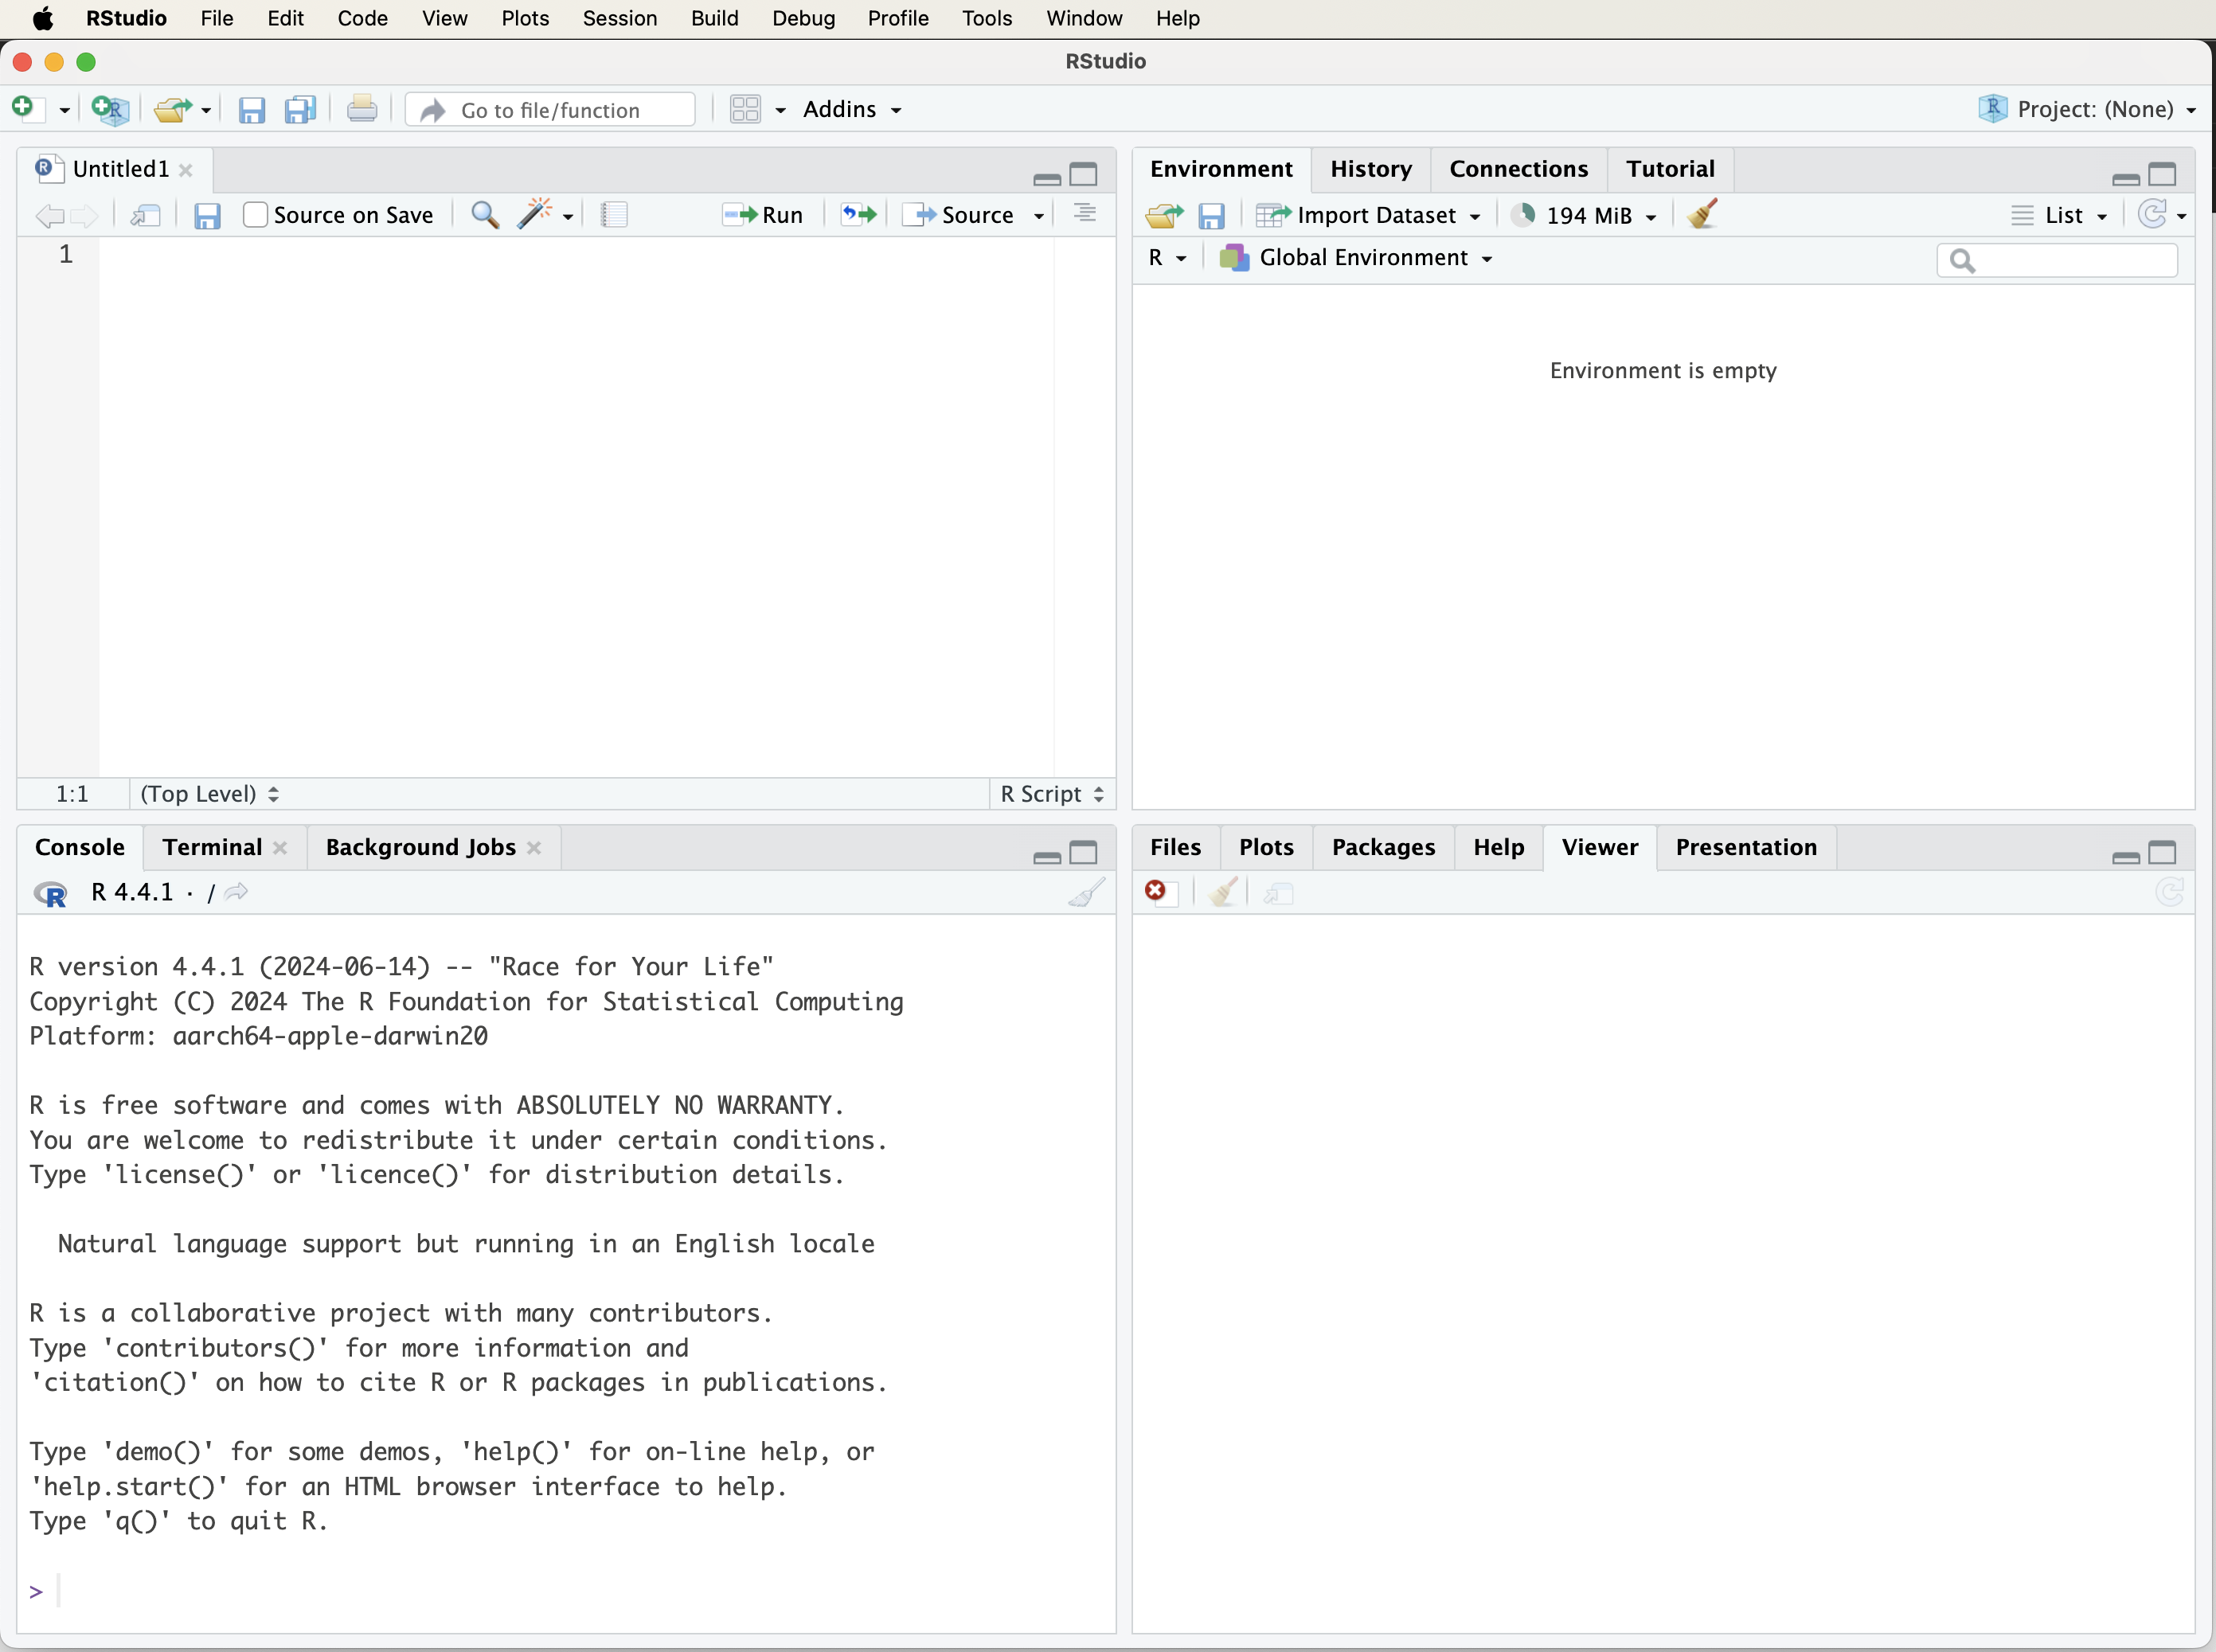
\includegraphics[width=0.7\linewidth]{images/RStudio-window-1} 

}

\caption{The RStudio window when you first launch the program.}\label{fig:RStudio-window-1}
\end{figure}

If you see only three panels, add a fourth by selecting \emph{File \textgreater{} New File \textgreater{} R Script}. This opens a script editor where you can write and save R code. Here's a quick overview of RStudio's panels:

\begin{itemize}
\tightlist
\item
  Top-left: Script Editor -- Write and save your R code.\\
\item
  Bottom-left: Console -- Run R commands and see output.\\
\item
  Top-right: Environment \& History -- View variables, datasets, and past commands.\\
\item
  Bottom-right: Plots, Help, \& Files -- Display graphs, access documentation, and manage files.
\end{itemize}

For now, just know that you can type R code into the console and press Enter to run it. As you progress through the book, you'll become more familiar with RStudio's features and learn how to efficiently write, run, and debug R code.

\subsection*{Customizing RStudio}\label{customizing-rstudio}
\addcontentsline{toc}{subsection}{Customizing RStudio}

RStudio is highly customizable, allowing you to tailor it to your workflow. To adjust settings, go to:

\begin{itemize}
\tightlist
\item
  Tools \textgreater{} Global Options -- Access general settings.\\
\item
  Appearance \textgreater{} Editor Theme -- Change the editor's theme (e.g., ``Tomorrow Night 80'' for a dark mode).\\
\item
  Font \& Layout Settings -- Modify font size, panel positions, and other interface options.\\
  A comfortable coding environment enhances productivity---so feel free to explore and tweak the settings to suit your preferences!
\end{itemize}

\section{How to Learn R}\label{how-to-learn-r}

Learning R is an exciting and rewarding journey that opens doors to data science, statistics, and machine learning. Fortunately, there are numerous resources---books, online courses, tutorials, and forums---that can help you get started and advance your skills.

\subsection*{1. Video Tutorials}\label{video-tutorials}
\addcontentsline{toc}{subsection}{1. Video Tutorials}

If you prefer learning by watching, YouTube offers a wealth of R tutorials, ranging from beginner to advanced levels:

\begin{itemize}
\tightlist
\item
  \href{https://www.youtube.com/channel/UCJ7w9dVjTOJi8Z7j0y9v6Qw}{R Programming} -- Covers R basics and data science concepts.\\
\item
  \href{https://www.youtube.com/user/dataschool}{Data School} -- Focuses on data analysis, machine learning, and practical R applications.
\end{itemize}

\subsection*{2. Books}\label{books}
\addcontentsline{toc}{subsection}{2. Books}

Books are a great way to build a deep understanding of R. Here are some top recommendations:

\begin{itemize}
\tightlist
\item
  For Absolute Beginners: \href{https://rstudio-education.github.io/hopr/}{\emph{Hands-On Programming with R}} by Garrett Grolemund\citep{grolemund2014hands} -- A practical introduction for those new to programming.\\
\item
  For Data Science with R: \href{https://r4ds.had.co.nz}{\emph{R for Data Science}} by Hadley Wickham and Garrett Grolemund \citep{wickham2017r} -- Covers data visualization, wrangling, and modeling.\\
\item
  For Machine Learning: \href{https://www.packtpub.com/product/machine-learning-with-r/9781782162148}{\emph{Machine Learning with R}} by Brett Lantz\citep{lantz2013machine} -- A comprehensive guide to machine learning techniques using R.
\end{itemize}

\subsection*{3. Online Courses}\label{online-courses}
\addcontentsline{toc}{subsection}{3. Online Courses}

If you prefer structured learning with hands-on exercises, online courses offer interactive experiences:

\begin{itemize}
\tightlist
\item
  \href{https://www.datacamp.com}{DataCamp} -- Features beginner-friendly courses like \href{https://learn.datacamp.com/courses/free-introduction-to-r}{\emph{Introduction to R}}.\\
\item
  \href{https://www.coursera.org}{Coursera} -- Offers courses such as \href{https://www.coursera.org/learn/r-programming}{\emph{R Programming}} and the \href{https://www.coursera.org/specializations/jhu-data-science}{\emph{Data Science Specialization}}.
\end{itemize}

\subsection*{4. R Communities \& Forums}\label{r-communities-forums}
\addcontentsline{toc}{subsection}{4. R Communities \& Forums}

Engaging with online communities is a great way to learn from others, ask questions, and get support:

\begin{itemize}
\tightlist
\item
  \href{https://stackoverflow.com/questions/tagged/r}{Stack Overflow} -- Find answers to R-related coding questions.\\
\item
  \href{https://community.rstudio.com/}{RStudio Community} -- Connect with other R users and participate in discussions.
\end{itemize}

\subsection*{5. Practice Regularly}\label{practice-regularly}
\addcontentsline{toc}{subsection}{5. Practice Regularly}

The best way to learn R is through consistent practice. Start with simple exercises, explore real-world datasets, and experiment with R code. By combining structured learning with hands-on experience, you'll quickly develop confidence and proficiency in R.

🚀 Start today! Choose one of the resources above and begin your R learning journey.

\section{Getting Help and Learning More}\label{getting-help-and-learning-more}

As you begin your journey with R, you'll likely encounter challenges and questions along the way. Fortunately, there are many resources available to help you troubleshoot problems, deepen your understanding, and continue learning. Whether you're stuck on an error message, exploring a new function, or looking for best practices, a combination of built-in documentation, online communities, and external learning materials can guide you.

R comes with extensive built-in documentation that provides details on functions, packages, and programming techniques. To quickly look up a function, type \passthrough{\lstinline!?!} followed by the function name in the R console. This will bring up official documentation, including usage examples, argument details, and additional references. You can also use \passthrough{\lstinline!help()!} or \passthrough{\lstinline!example()!} to get more context on how a function works.

Beyond R's internal help system, the R community is an invaluable resource. If you have a question, chances are someone has already asked (and answered) it. Platforms like Stack Overflow, RStudio Community, and the R-help mailing list contain thousands of discussions on common and advanced topics in R programming, data science, and machine learning. Searching these forums can often lead you to quick and reliable solutions. If you don't find an existing answer, posting your question with a clear explanation and a reproducible example will increase your chances of getting helpful responses.

A simple Google search is often the fastest way to troubleshoot issues. Searching for an error message or function name will usually direct you to blog posts, documentation, or forum discussions with relevant explanations. Additionally, AI tools like ChatGPT can assist with R programming questions, debugging, and conceptual explanations. While AI-generated solutions aren't always perfect, they can provide useful insights, suggest alternative approaches, and help clarify difficult concepts.

Ultimately, the best way to master R is through hands-on experience. Don't be afraid to experiment---write code, test different functions, and explore new datasets. Mistakes are a natural part of learning, and each one helps reinforce your understanding. The more you practice, the more confident and proficient you'll become in R. Keep coding, keep exploring, and enjoy the journey!

\section{Data Science with R}\label{data-science-with-r}

R provides a strong foundation for data science, but its real power comes from its extensive ecosystem of packages---collections of functions, datasets, and documentation that extend R's capabilities. While the base version of R includes many essential tools, it does not come preloaded with all the statistical and machine learning algorithms you may need. Instead, these algorithms are developed and shared by a large community of researchers and practitioners as free and open-source R packages.

A package is a modular, reusable library that enhances R's functionality. Packages include well-documented functions, usage instructions, and often sample datasets for testing and learning. In this book, we frequently use the \textbf{liver} package, which was developed specifically to accompany this book. It contains datasets and functions designed to illustrate key data science concepts and techniques. Additionally, for each machine learning algorithm covered in this book, we introduce and use the appropriate R packages that implement those methods.

For those interested in exploring further, the Comprehensive R Archive Network (CRAN) hosts thousands of packages for statistical computing, data visualization, and machine learning. The full list of available packages can be browsed on the \href{https://CRAN.R-project.org}{CRAN website}, providing access to tools tailored to various domains in data science and beyond.

\section{How to Install R Packages}\label{install-packages}

There are two ways to install R packages. The first method is through RStudio's graphical interface. Click on the ``Tools'' tab and select ``Install Packages\ldots{}''. In the dialog box that appears, enter the name of the package(s) you wish to install in the ``Packages'' field and click the ``Install'' button. Make sure to check the ``Install dependencies'' option to ensure that all necessary supporting packages are installed as well. See Figure \ref{fig:install-packages} for a visual guide.

\begin{figure}

{\centering 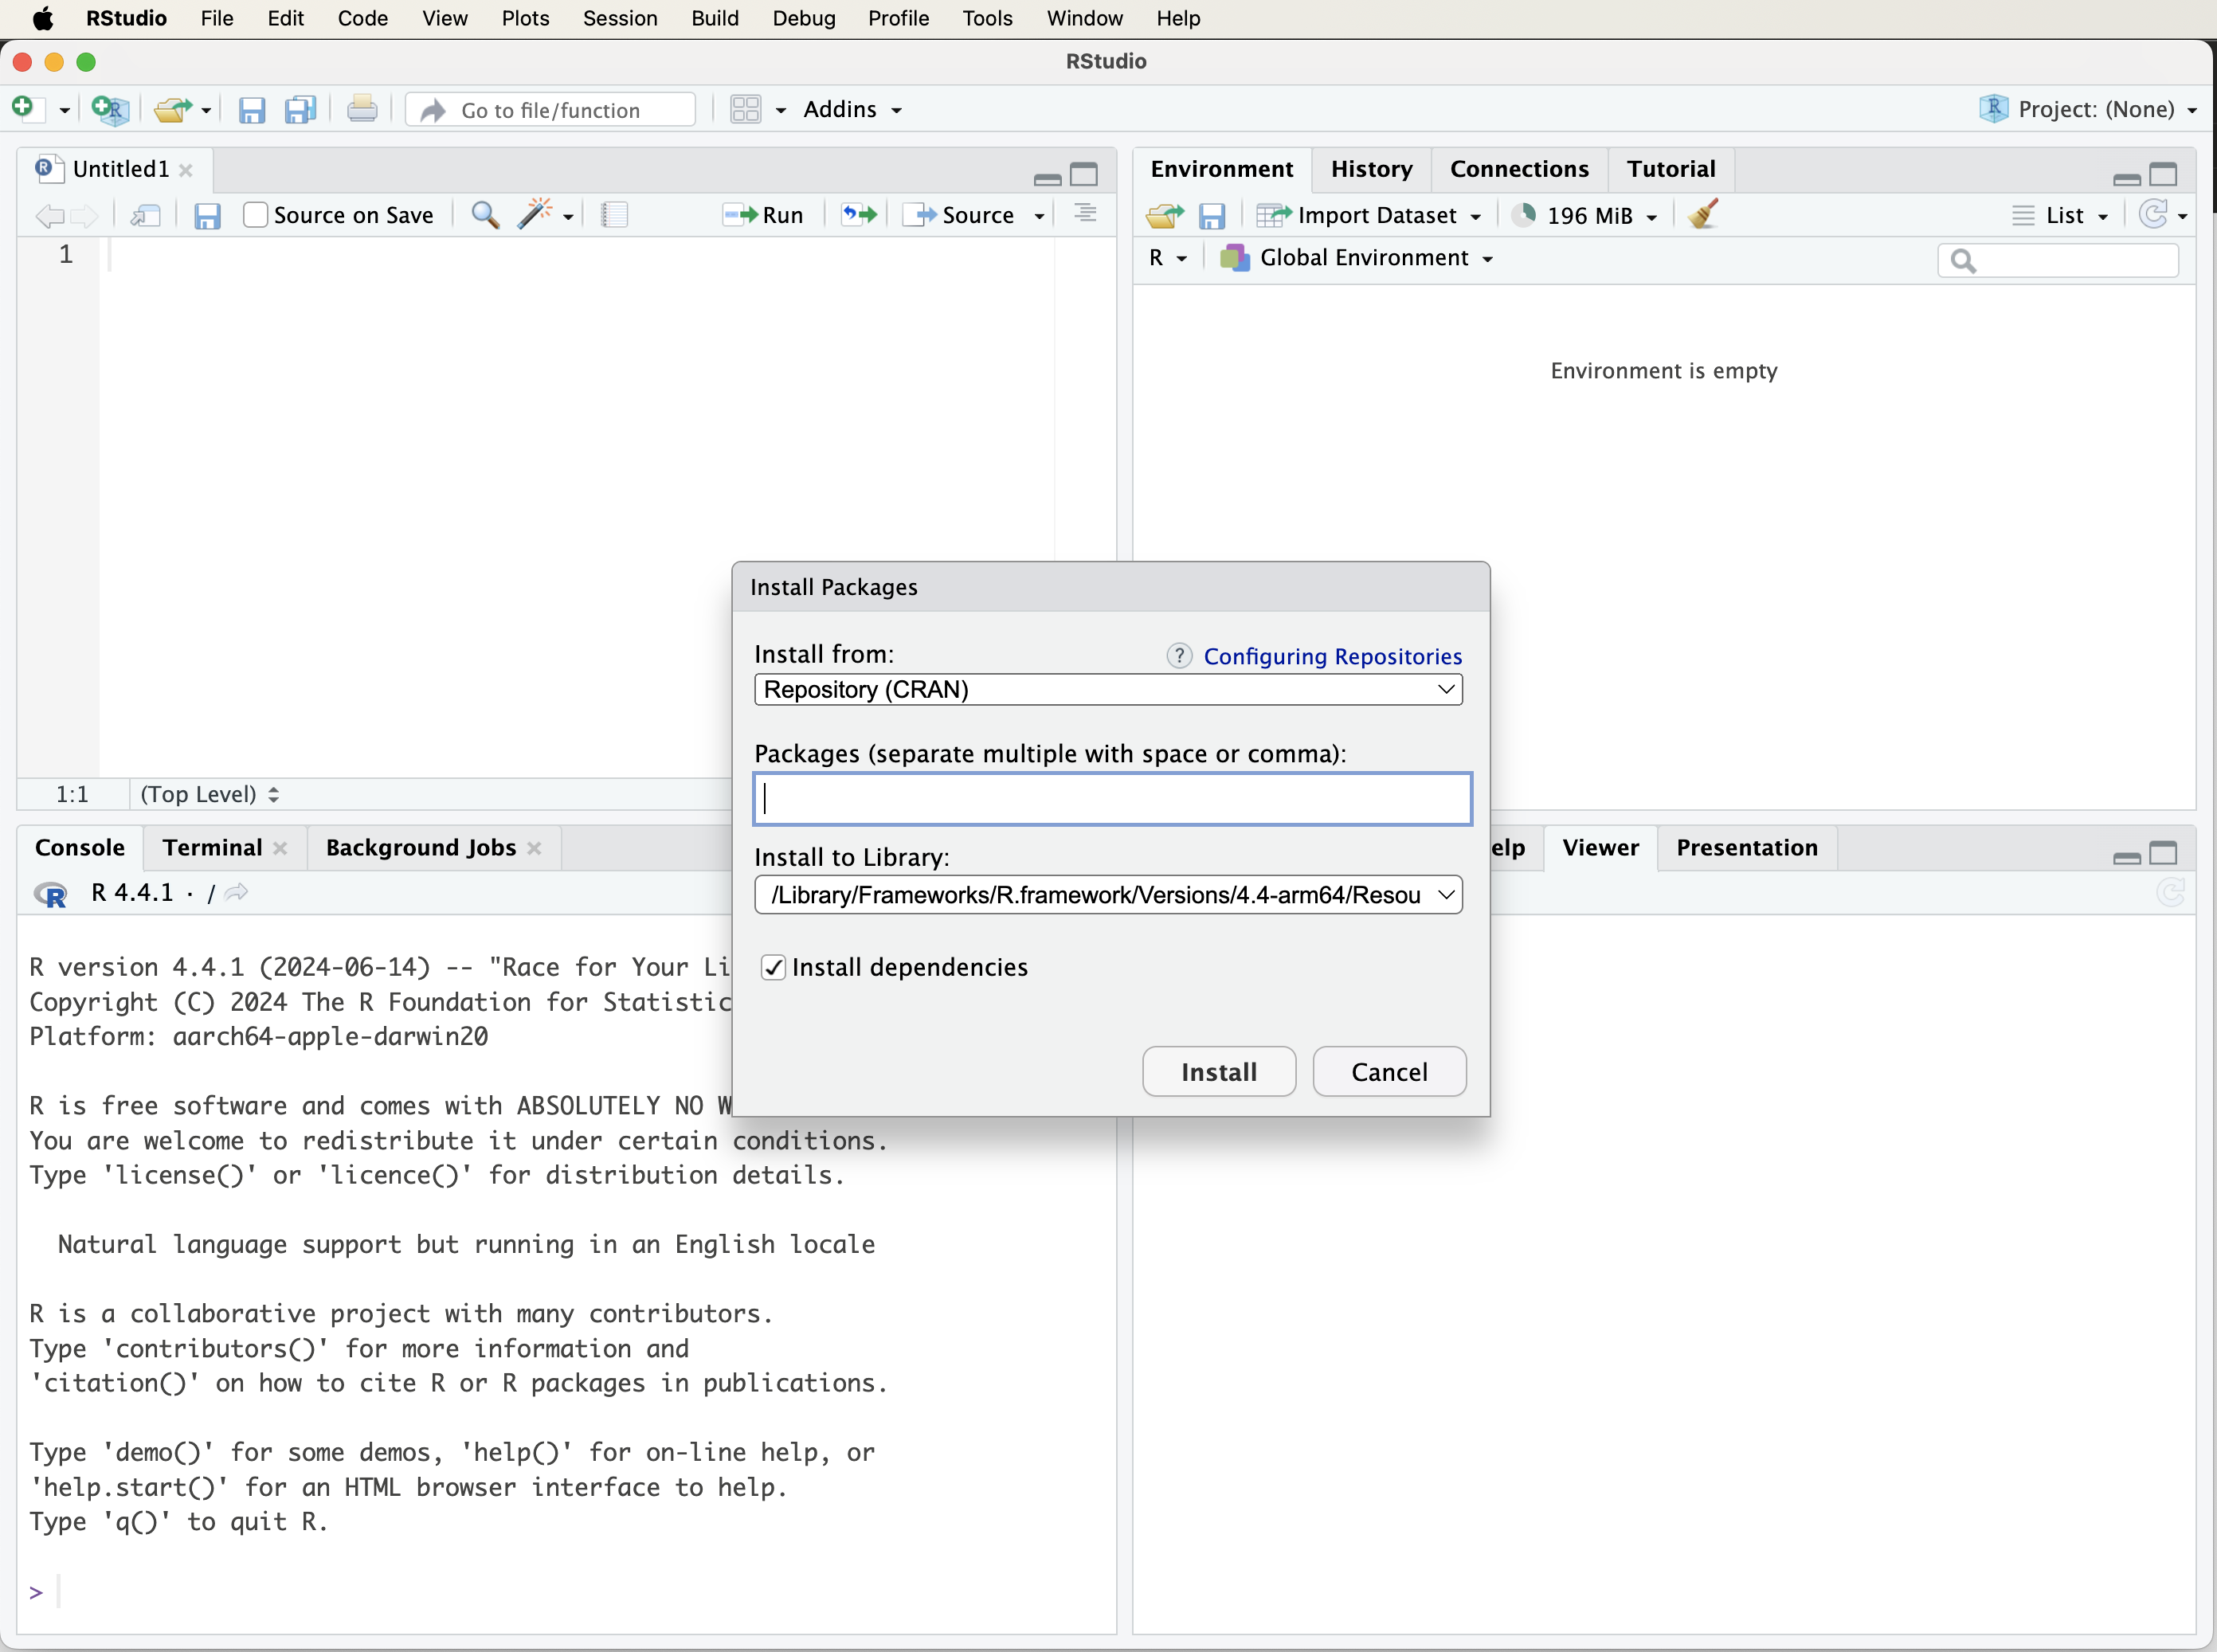
\includegraphics[width=0.7\linewidth]{images/RStudio-window-install} 

}

\caption{A visual guide to installing R packages using the 'Tools' tab in RStudio.}\label{fig:install-packages}
\end{figure}

The second method is to install packages directly using the \passthrough{\lstinline!install.packages()!} function. For example, to install the \textbf{liver} package, which provides datasets and functions used throughout this book, enter the following command in the R console:

\begin{lstlisting}[language=R]
install.packages("liver")
\end{lstlisting}

Press ``Enter'' to execute the command. R will connect to \href{https://cran.r-project.org}{CRAN} and download the package in the correct format for your operating system. If you encounter any issues during installation, ensure you are connected to the internet and that your proxy or firewall is not blocking access to CRAN. The first time you install a package, R may ask you to select a CRAN mirror. Choose one that is geographically close to you for faster downloads.

The \passthrough{\lstinline!install.packages()!} function also allows for customization, such as installing a package from a local file or a specific repository. To learn more, type the following command in the R console:

\begin{lstlisting}[language=R]
?install.packages()
\end{lstlisting}

Packages only need to be installed once. After installation, they must be loaded into each new R session using the \passthrough{\lstinline!library()!} function. We will cover how to load packages in the next section.

\section{How to Load R Packages}\label{how-to-load-r-packages}

To optimize memory usage, R does not automatically load all installed packages. Instead, you must explicitly load the necessary packages in each new R session. This ensures that only relevant functions and datasets are available, minimizing resource consumption.\\
To load a package, use the \passthrough{\lstinline!library()!} or \passthrough{\lstinline!require()!} function. These functions locate the package on your system and make its functions, datasets, and documentation accessible. For example, to load the \textbf{liver} package, enter the following command in the R console:

\begin{lstlisting}[language=R]
library(liver)
\end{lstlisting}

Press \emph{Enter} to execute the command. If an error message appears stating that the package is not found (e.g., \passthrough{\lstinline!"there is no package called 'liver'"!}), it indicates that the package has not been installed. In such cases, refer to the previous section on installing packages.

Beyond \textbf{liver}, this book utilizes several other R packages, which will be introduced progressively throughout the chapters as needed. However, some R packages contain functions with identical names. For instance, both the \textbf{liver* and }dplyr** packages include a \passthrough{\lstinline!select()!} function. When multiple packages are loaded, R defaults to using the function from the most recently loaded package.

To explicitly specify which package a function should be sourced from, use the \passthrough{\lstinline!::!} operator. This ensures clarity and prevents conflicts. For example, to use the \passthrough{\lstinline!select()!} function from the \textbf{liver} package, enter:

\begin{lstlisting}[language=R]
liver::select()
\end{lstlisting}

This approach is particularly useful in complex projects where multiple packages are required, preventing unintended overwrites of functions with the same name.

\section{Running R Code}\label{running-r-code}

R is an interactive language, allowing you to type commands directly into the console and see the results immediately. For example, you can perform basic arithmetic operations such as addition, subtraction, multiplication, and division. To add two numbers, type the following in the R console:

\begin{lstlisting}[language=R]
2 + 3
   [1] 5
\end{lstlisting}

Press \emph{Enter} to execute the command. R will compute the sum and display the result. You can also store this result in a variable for later use:

\begin{lstlisting}[language=R]
result <- 2 + 3
\end{lstlisting}

Here, \passthrough{\lstinline!<-!} is the assignment operator in R, used to assign values to variables. Some users prefer the \passthrough{\lstinline!=!} operator (\passthrough{\lstinline!result = 2 + 3!}), which also works in most cases, but \passthrough{\lstinline!<-!} remains the recommended convention in R programming.

Variables in R store values for later use, allowing you to perform calculations efficiently. For example, you can multiply \passthrough{\lstinline!result!} by 4:

\begin{lstlisting}[language=R]
result * 4
   [1] 20
\end{lstlisting}

R will retrieve the stored value of \passthrough{\lstinline!result!} and compute the multiplication.

\subsection*{Using Comments in R}\label{using-comments-in-r}
\addcontentsline{toc}{subsection}{Using Comments in R}

Comments are used to explain your code and make it easier to understand. In R, a comment starts with \passthrough{\lstinline!\#!}, and everything following it on that line is ignored by the interpreter.

\begin{lstlisting}[language=R]
# Store the sum of 2 and 3 in the variable `result`
result <- 2 + 3
\end{lstlisting}

Comments do not affect the execution of your code but are essential for documentation, especially when working on complex projects or collaborating with others.

\subsection{Functions in R}\label{functions-in-r}

R provides a rich set of built-in functions to perform specific tasks. A function takes \textbf{input(s)} (arguments), processes them, and returns an \textbf{output}. For example, the \passthrough{\lstinline!c()!} function creates vectors:

\begin{lstlisting}[language=R]
x <- c(1, 2, 3, 4, 5)  # Create a vector
\end{lstlisting}

You can then apply functions to this vector. For example, to compute the average of the numbers in \passthrough{\lstinline!x!}, use the \passthrough{\lstinline!mean()!} function:

\begin{lstlisting}[language=R]
mean(x)  # Calculate the mean of x
   [1] 3
\end{lstlisting}

Functions in R follow a simple structure:

\begin{lstlisting}[language=R]
function_name(arguments)
\end{lstlisting}

Some functions require arguments, while others are optional. To learn more about a function, use \passthrough{\lstinline!?!} followed by the function name:

\begin{lstlisting}[language=R]
?mean  # or help(mean)
\end{lstlisting}

This will open R's help documentation, providing details about the function's purpose, usage, arguments, and examples.

Functions are essential in R programming, helping to simplify complex operations and making code more reusable and efficient. As you progress, you will also learn how to write your own functions to automate tasks and improve workflow.

\section{How to Import Data into R}\label{how-to-import-data-into-r}

Before performing any analysis, you first need to load data into R. R can read data from multiple sources, including text files, Excel files, and online datasets. Depending on the file format and data source, you can choose from several methods for importing data into R.

\subsection*{Using RStudio's Graphical Interface}\label{using-rstudios-graphical-interface}
\addcontentsline{toc}{subsection}{Using RStudio's Graphical Interface}

The easiest way to import data into R is through RStudio's graphical interface. Click on the \emph{Import Dataset} button in the top-right panel of RStudio (see Figure \ref{fig:load-data} for a visual guide). This will open a dialog box where you can choose the file type:\\
- \textbf{From Text (base)} -- for CSV or tab-delimited files.\\
- \textbf{From Excel} -- for Microsoft Excel files.\\
- Other formats are available, depending on installed packages.

After selecting your file, RStudio will display an import settings window (see Figure \ref{fig:load-data-2}). Here, you can adjust column names, data types, and other options. If the first row contains column names, select \emph{Yes} under the \emph{Heading} option. Click \emph{Import}, and the dataset will appear in RStudio's Environment panel, ready for analysis.

\begin{figure}

{\centering 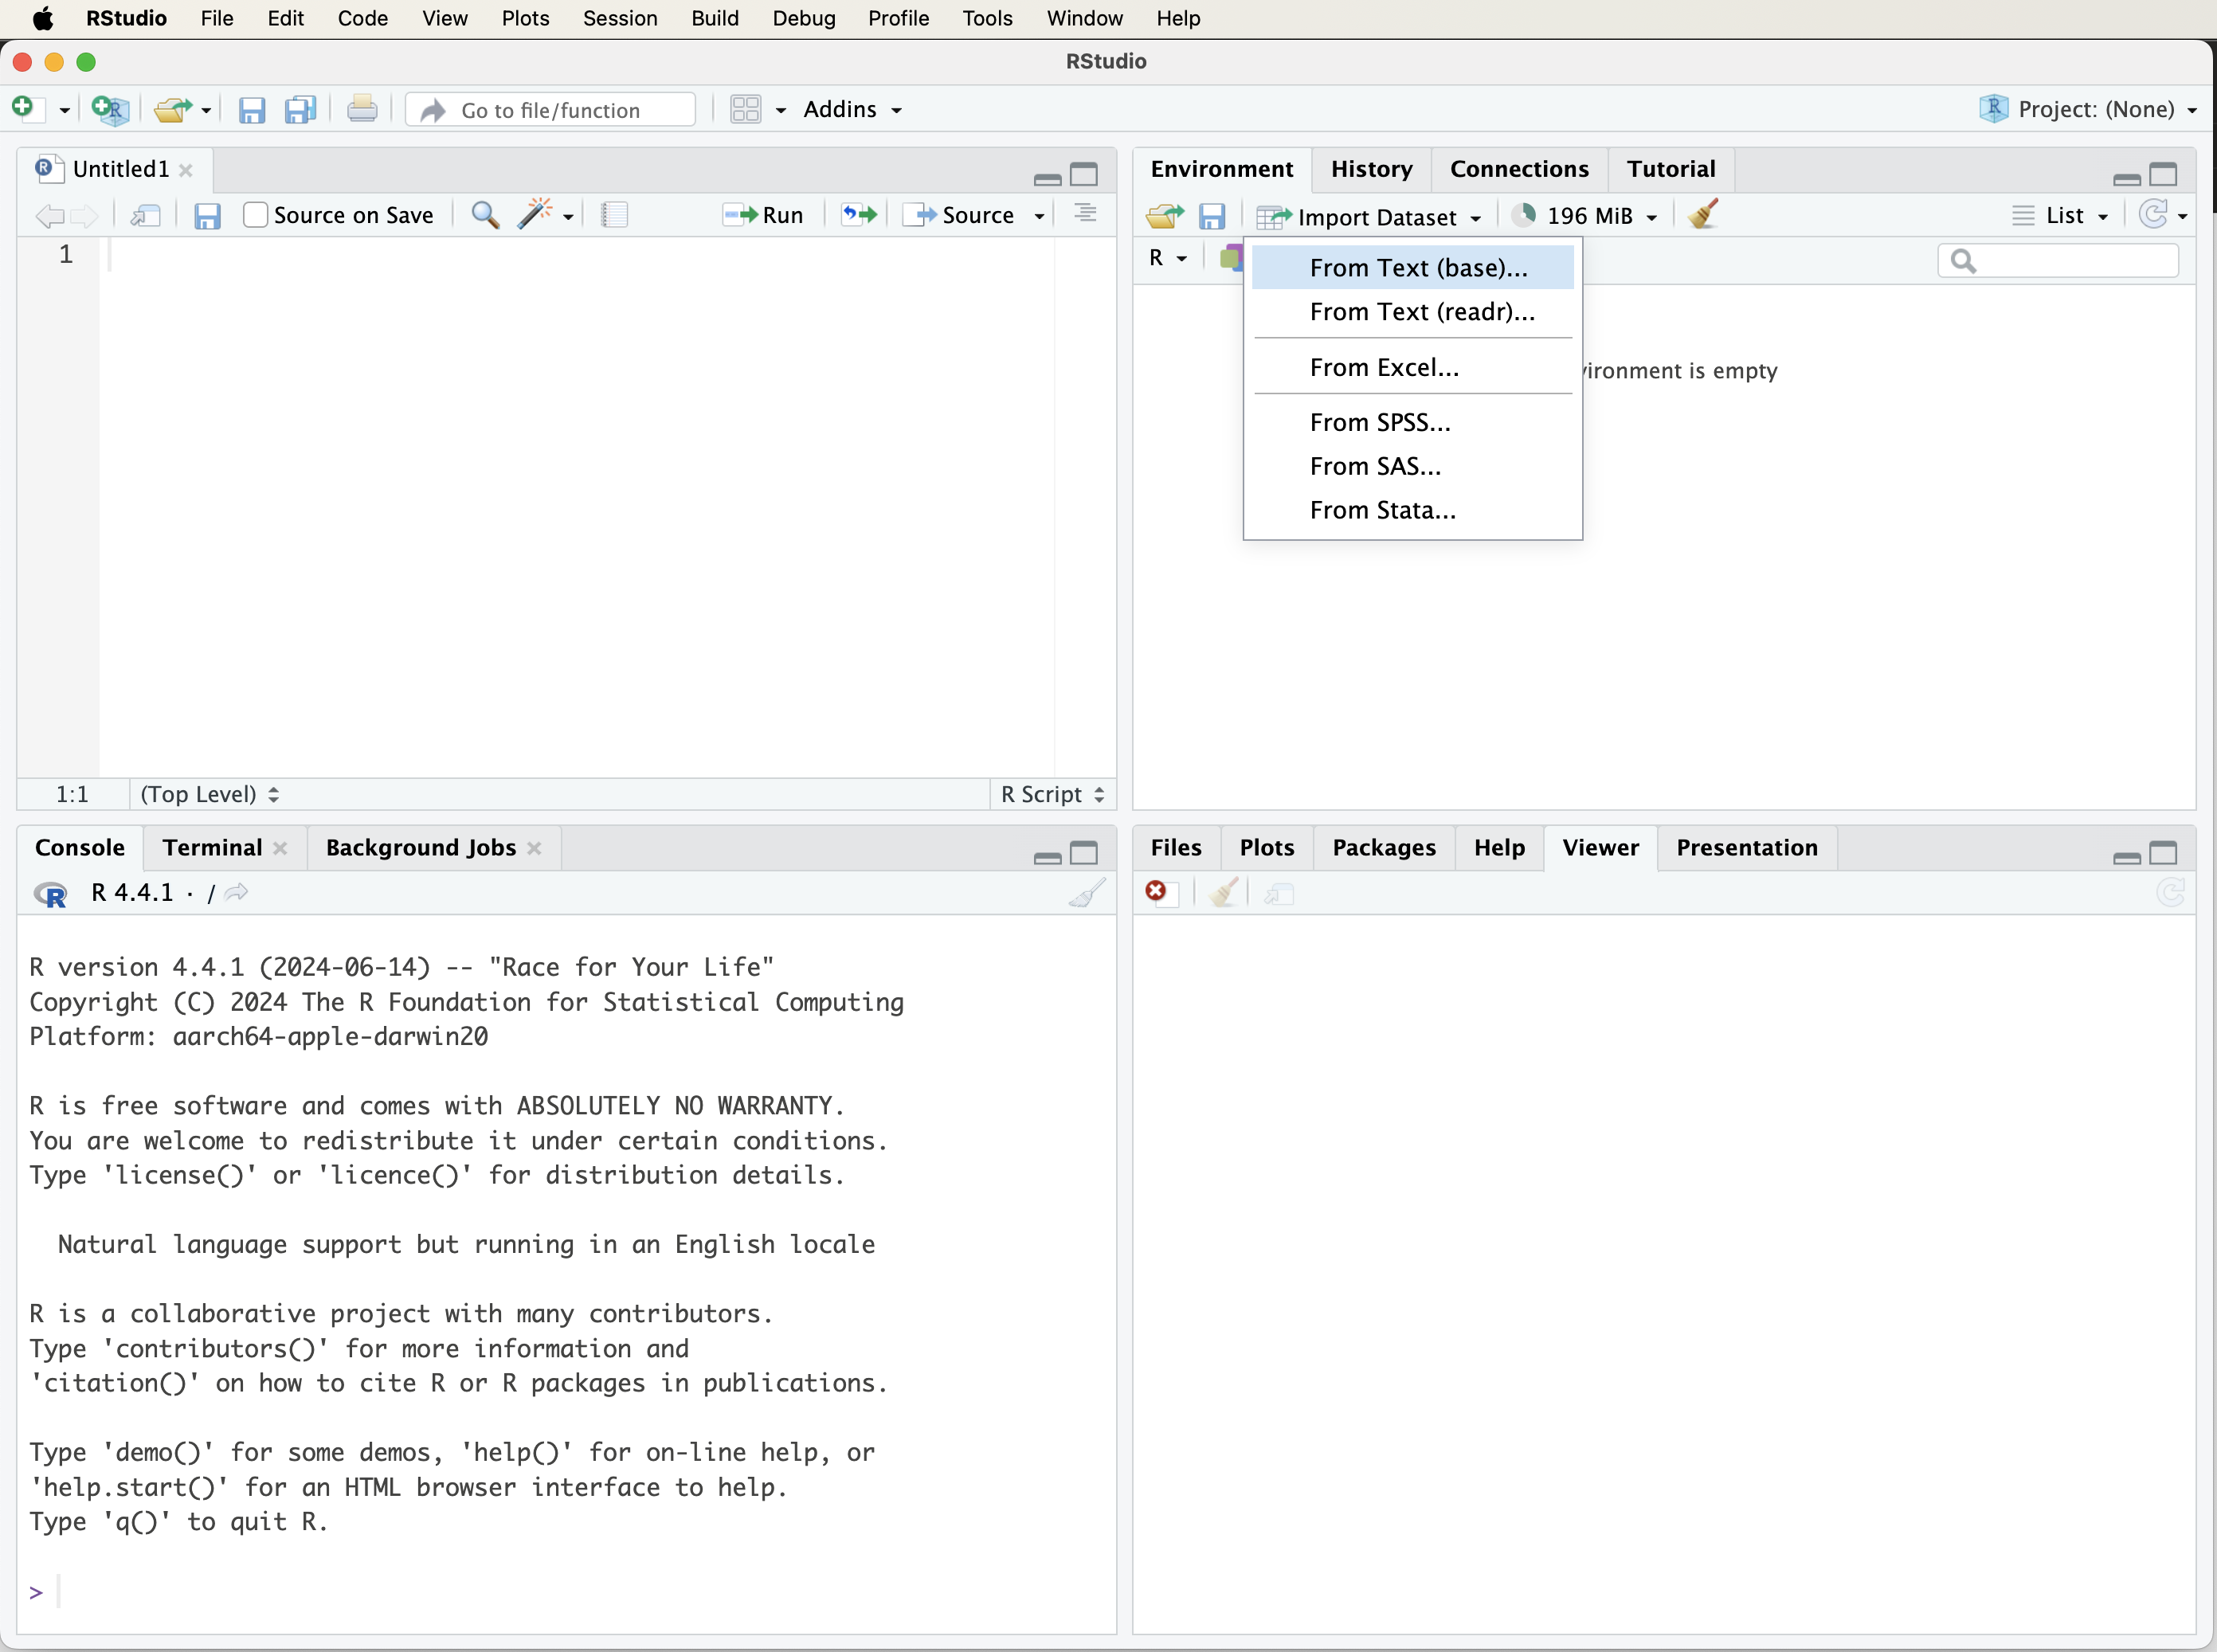
\includegraphics[width=0.7\linewidth]{images/RStudio-window-data-1} 

}

\caption{A visual guide to loading a dataset into R using the 'Import Dataset' tab in RStudio.}\label{fig:load-data}
\end{figure}

\begin{figure}

{\centering 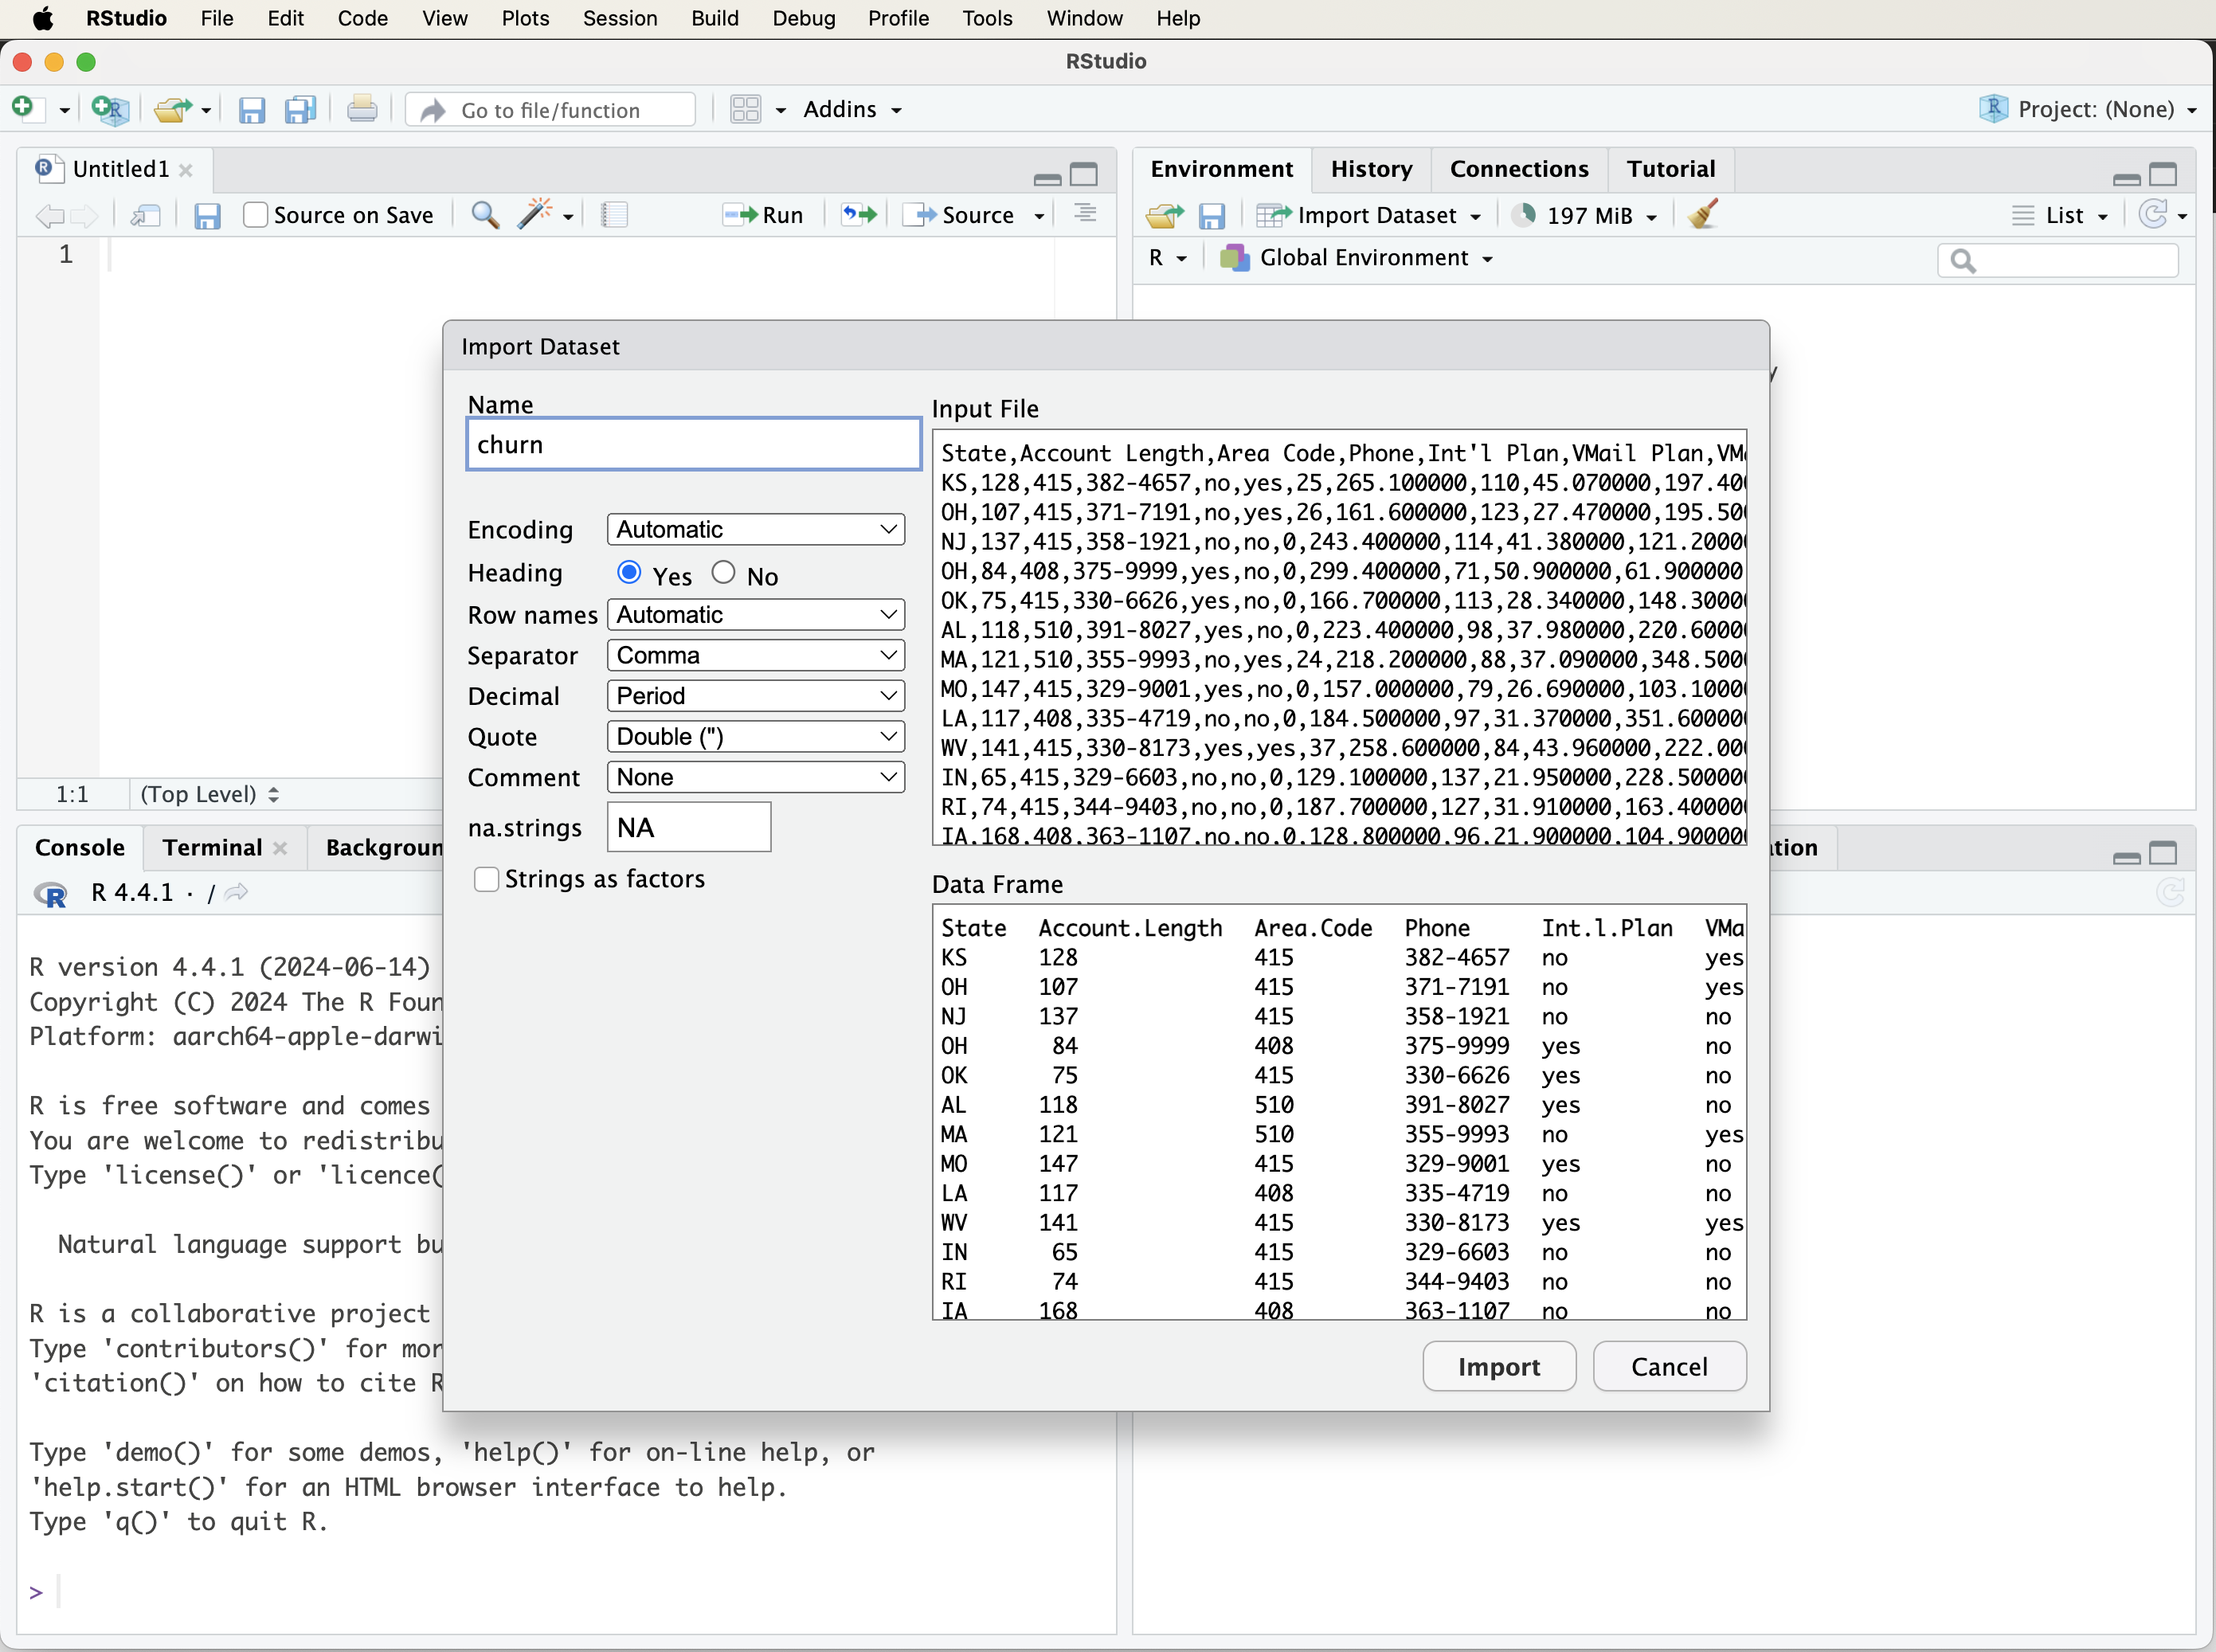
\includegraphics[width=0.7\linewidth]{images/RStudio-window-data} 

}

\caption{A visual guide to customizing the import settings when loading a dataset into R using the 'Import Dataset' tab in RStudio.}\label{fig:load-data-2}
\end{figure}

\subsection*{\texorpdfstring{Using \texttt{read.csv()}}{Using read.csv()}}\label{using-read.csv}
\addcontentsline{toc}{subsection}{Using \texttt{read.csv()}}

You can also import data directly using the \passthrough{\lstinline!read.csv()!} function, which reads tabular data (such as CSV files) into R as a data frame. If your data file is stored locally, you can load it as follows:

\begin{lstlisting}[language=R]
data <- read.csv("path/to/your/file.csv")
\end{lstlisting}

Replace \passthrough{\lstinline!"path/to/your/file.csv"!} with the actual file path. If your file does not contain column names, use:

\begin{lstlisting}[language=R]
data <- read.csv("path/to/your/file.csv", header = FALSE)
\end{lstlisting}

\subsection*{Setting the Working Directory}\label{setting-the-working-directory}
\addcontentsline{toc}{subsection}{Setting the Working Directory}

By default, R looks for files in the current working directory. If your data is located elsewhere, you can specify the full path in \passthrough{\lstinline!read.csv()!} or set the working directory.

To check your current working directory:

\begin{lstlisting}[language=R]
getwd()
\end{lstlisting}

To set a new working directory:

\begin{lstlisting}[language=R]
setwd("~/Documents")  # Adjust the path based on your system
\end{lstlisting}

Alternatively, in RStudio, go to \emph{Session \textgreater{} Set Working Directory \textgreater{} Choose Directory\ldots{}} and select the desired folder.

\subsection*{\texorpdfstring{Using \texttt{file.choose()} with \texttt{read.csv()}}{Using file.choose() with read.csv()}}\label{using-file.choose-with-read.csv}
\addcontentsline{toc}{subsection}{Using \texttt{file.choose()} with \texttt{read.csv()}}

To interactively select a file instead of typing its path manually, use \passthrough{\lstinline!file.choose()!}:

\begin{lstlisting}[language=R]
data <- read.csv(file.choose())
\end{lstlisting}

This will open a file selection dialog, making it a convenient option when working with multiple datasets.

\subsection*{Loading Data from Online Sources}\label{loading-data-from-online-sources}
\addcontentsline{toc}{subsection}{Loading Data from Online Sources}

R also allows direct import of datasets from web sources. For example, to load a publicly available COVID-19 dataset:

\begin{lstlisting}[language=R]
corona_data <- read.csv("https://opendata.ecdc.europa.eu/covid19/casedistribution/csv", na.strings = "", fileEncoding = "UTF-8-BOM")
\end{lstlisting}

This approach is useful for accessing open datasets from research institutions or government agencies.

\subsection*{\texorpdfstring{Using \texttt{read\_excel()} for Excel Files}{Using read\_excel() for Excel Files}}\label{using-read_excel-for-excel-files}
\addcontentsline{toc}{subsection}{Using \texttt{read\_excel()} for Excel Files}

To import Excel files, use the \passthrough{\lstinline!read\_excel()!} function from the \textbf{readxl} package. First, install and load the package:

\begin{lstlisting}[language=R]
install.packages("readxl")

library(readxl)
\end{lstlisting}

Then, import the Excel file:

\begin{lstlisting}[language=R]
data <- read_excel("path/to/your/file.xlsx")
\end{lstlisting}

Unlike \passthrough{\lstinline!read.csv()!}, \passthrough{\lstinline!read\_excel()!} supports multiple sheets within an Excel file, which can be specified using the \passthrough{\lstinline!sheet!} argument.\\
\#\#\# Loading Data from R Packages \{-\}

Some datasets are available directly in R packages and do not require importing from an external file. For example, the \textbf{liver} package, developed for this book, contains multiple datasets. To access the \emph{churn} dataset:

\begin{lstlisting}[language=R]
library(liver)
data(churn)
\end{lstlisting}

Since many of the datasets used in this book are included in the \textbf{liver} package (see Table \ref{tab:data-table}), we will frequently use this package for examples and demonstrations.

This section is well-structured and clearly explains the fundamental data types in R. It is concise and informative, making it accessible to beginners while maintaining a professional tone suitable for a Springer publication. Below are some minor refinements to improve clarity, consistency, and readability.

\section{Data Types in R}\label{data-types-in-r}

Data in R can take various forms, and correctly identifying these types is essential for effective data manipulation, visualization, and analysis. Each data type has specific properties that determine how R processes it, so understanding them helps avoid errors and ensures accurate results.

Here are the most common data types in R:

\begin{itemize}
\tightlist
\item
  \textbf{Numeric}: Represents real numbers, such as \passthrough{\lstinline!3.14!} or \passthrough{\lstinline!-5.67!}. This type is used for continuous numerical values, like heights, weights, or temperatures.\\
\item
  \textbf{Integer}: Represents whole numbers without decimals, such as \passthrough{\lstinline!1!}, \passthrough{\lstinline!42!}, or \passthrough{\lstinline!-10!}. This type is useful for count-based data, such as the number of customers or items sold.\\
\item
  \textbf{Character}: Represents text or string data, such as \passthrough{\lstinline!"Data Science"!} or \passthrough{\lstinline!"R Programming"!}. This type is commonly used for categorical labels, names, and descriptive values.\\
\item
  \textbf{Logical}: Represents Boolean values: \passthrough{\lstinline!TRUE!} or \passthrough{\lstinline!FALSE!}. Logical data is often used in conditional statements and filtering operations.\\
\item
  \textbf{Factor}: Represents categorical data with predefined levels. Factors are commonly used for storing variables such as \passthrough{\lstinline!"Male"!} or \passthrough{\lstinline!"Female"!} in a dataset and are particularly useful in statistical modeling.
\end{itemize}

To check the data type of a variable, use the \passthrough{\lstinline!class()!} function. For example, to determine the type of the variable \passthrough{\lstinline!result!}, type:

\begin{lstlisting}[language=R]
class(result)
   [1] "numeric"
\end{lstlisting}

Press \emph{Enter}, and R will display the variable's data type.

Recognizing different data types is essential for choosing the right analytical and visualization techniques. As we will explore in later chapters (e.g., Chapters \ref{chapter-EDA} and \ref{chapter-statistics}), numerical and categorical variables require different approaches when performing descriptive statistics, hypothesis testing, and data visualization.

\section{Data Structures in R}\label{data-structures-in-r}

Data structures are fundamental to working with data in R. They define how data is stored and manipulated, which directly impacts the efficiency and accuracy of data analysis. The most commonly used data structures in R are vectors, matrices, data frames, and lists, as illustrated in Figure \ref{fig:load-data-2}.

\begin{figure}

{\centering 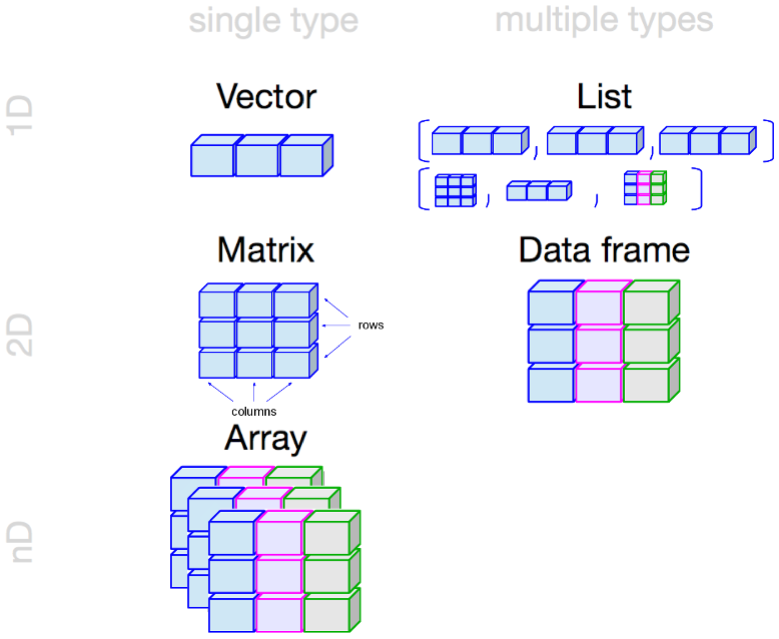
\includegraphics[width=0.6\linewidth]{images/R-objects} 

}

\caption{A visual guide to different types of data structures in R.}\label{fig:R-objects}
\end{figure}

\subsection*{Vectors in R}\label{vectors-in-r}
\addcontentsline{toc}{subsection}{Vectors in R}

A vector is the simplest data structure in R. It is a one-dimensional array that holds elements of the same type (numeric, character, or logical). Vectors are the building blocks of other data structures. You can create a vector using the \passthrough{\lstinline!c()!} function:

\begin{lstlisting}[language=R]
# Create a numeric vector
x <- c(1, 2, 0, -3, 5)

# Display the vector
x
   [1]  1  2  0 -3  5

# Check if x is a vector
is.vector(x)
   [1] TRUE

# Check the length of the vector
length(x)
   [1] 5
\end{lstlisting}

Here, \passthrough{\lstinline!x!} is a numeric vector containing five elements. The \passthrough{\lstinline!is.vector()!} function confirms that \passthrough{\lstinline!x!} is indeed a vector, while \passthrough{\lstinline!length(x)!} returns the number of elements in the vector.

\subsection*{Matrices in R}\label{matrices-in-r}
\addcontentsline{toc}{subsection}{Matrices in R}

A matrix is a two-dimensional array where all elements must be of the same type. Matrices are useful for mathematical operations and structured numerical data. You can create a matrix using the \passthrough{\lstinline!matrix()!} function:

\begin{lstlisting}[language=R]
# Create a matrix with 2 rows and 3 columns
m <- matrix(c(1, 2, 3, 4, 5, 6), nrow = 2, ncol = 3, byrow = TRUE)

# Display the matrix
m
        [,1] [,2] [,3]
   [1,]    1    2    3
   [2,]    4    5    6

# Check if m is a matrix
is.matrix(m)
   [1] TRUE

# Check the dimensions of the matrix
dim(m)
   [1] 2 3
\end{lstlisting}

This matrix \passthrough{\lstinline!m!} consists of two rows and three columns, filled row-wise. The \passthrough{\lstinline!dim()!} function returns the dimensions of the matrix. To fill the matrix column-wise, set \passthrough{\lstinline!byrow = FALSE!}.

\subsection*{Data Frames in R}\label{data-frames-in-r}
\addcontentsline{toc}{subsection}{Data Frames in R}

A data frame is a two-dimensional table where each column can contain a different data type (numeric, character, or logical). This makes data frames ideal for storing tabular data, similar to spreadsheets. You can create a data frame using the \passthrough{\lstinline!data.frame()!} function:

\begin{lstlisting}[language=R]
# Create vectors for student data
student_id <- c(101, 102, 103, 104)
name       <- c("Emma", "Bob", "Alice", "Noah")
age        <- c(20, 21, 19, 22)
grade      <- c("A", "B", "A", "C")

# Create a data frame from the vectors
students_df <- data.frame(student_id, name, age, grade)

# Display the data frame
students_df
     student_id  name age grade
   1        101  Emma  20     A
   2        102   Bob  21     B
   3        103 Alice  19     A
   4        104  Noah  22     C
\end{lstlisting}

This data frame \passthrough{\lstinline!students\_df!} consists of four columns: \passthrough{\lstinline!student\_id!}, \passthrough{\lstinline!name!}, \passthrough{\lstinline!age!}, and \passthrough{\lstinline!grade!}. The \passthrough{\lstinline!class()!} function confirms that an object is a data frame, while \passthrough{\lstinline!is.data.frame()!} checks its structure.

To inspect the first few rows of a data frame, use the \passthrough{\lstinline!head()!} function. For example, to display the first six rows of the \emph{churn} dataset from the \textbf{liver} package:

\begin{lstlisting}[language=R]
library(liver)  # Load the liver package
data(churn)     # Load the churn dataset

# Check the structure of the dataset
str(churn)
   'data.frame':    5000 obs. of  20 variables:
    $ state         : Factor w/ 51 levels "AK","AL","AR",..: 17 36 32 36 37 2 20 25 19 50 ...
    $ area.code     : Factor w/ 3 levels "area_code_408",..: 2 2 2 1 2 3 3 2 1 2 ...
    $ account.length: int  128 107 137 84 75 118 121 147 117 141 ...
    $ voice.plan    : Factor w/ 2 levels "yes","no": 1 1 2 2 2 2 1 2 2 1 ...
    $ voice.messages: int  25 26 0 0 0 0 24 0 0 37 ...
    $ intl.plan     : Factor w/ 2 levels "yes","no": 2 2 2 1 1 1 2 1 2 1 ...
    $ intl.mins     : num  10 13.7 12.2 6.6 10.1 6.3 7.5 7.1 8.7 11.2 ...
    $ intl.calls    : int  3 3 5 7 3 6 7 6 4 5 ...
    $ intl.charge   : num  2.7 3.7 3.29 1.78 2.73 1.7 2.03 1.92 2.35 3.02 ...
    $ day.mins      : num  265 162 243 299 167 ...
    $ day.calls     : int  110 123 114 71 113 98 88 79 97 84 ...
    $ day.charge    : num  45.1 27.5 41.4 50.9 28.3 ...
    $ eve.mins      : num  197.4 195.5 121.2 61.9 148.3 ...
    $ eve.calls     : int  99 103 110 88 122 101 108 94 80 111 ...
    $ eve.charge    : num  16.78 16.62 10.3 5.26 12.61 ...
    $ night.mins    : num  245 254 163 197 187 ...
    $ night.calls   : int  91 103 104 89 121 118 118 96 90 97 ...
    $ night.charge  : num  11.01 11.45 7.32 8.86 8.41 ...
    $ customer.calls: int  1 1 0 2 3 0 3 0 1 0 ...
    $ churn         : Factor w/ 2 levels "yes","no": 2 2 2 2 2 2 2 2 2 2 ...

# Display the first six rows
head(churn)
     state     area.code account.length voice.plan voice.messages intl.plan
   1    KS area_code_415            128        yes             25        no
   2    OH area_code_415            107        yes             26        no
   3    NJ area_code_415            137         no              0        no
   4    OH area_code_408             84         no              0       yes
   5    OK area_code_415             75         no              0       yes
   6    AL area_code_510            118         no              0       yes
     intl.mins intl.calls intl.charge day.mins day.calls day.charge eve.mins
   1      10.0          3        2.70    265.1       110      45.07    197.4
   2      13.7          3        3.70    161.6       123      27.47    195.5
   3      12.2          5        3.29    243.4       114      41.38    121.2
   4       6.6          7        1.78    299.4        71      50.90     61.9
   5      10.1          3        2.73    166.7       113      28.34    148.3
   6       6.3          6        1.70    223.4        98      37.98    220.6
     eve.calls eve.charge night.mins night.calls night.charge customer.calls churn
   1        99      16.78      244.7          91        11.01              1    no
   2       103      16.62      254.4         103        11.45              1    no
   3       110      10.30      162.6         104         7.32              0    no
   4        88       5.26      196.9          89         8.86              2    no
   5       122      12.61      186.9         121         8.41              3    no
   6       101      18.75      203.9         118         9.18              0    no
\end{lstlisting}

This code loads the \textbf{liver} package, retrieves the \emph{churn} dataset, and provides an overview of its structure. The \passthrough{\lstinline!str()!} function is particularly useful for summarizing data frames, as it displays data types and column values.

\subsection*{Lists in R}\label{lists-in-r}
\addcontentsline{toc}{subsection}{Lists in R}

A list is a flexible data structure that can contain elements of different types, including vectors, matrices, data frames, or even other lists. Lists are useful for storing complex objects in a structured way. You can create a list using the \passthrough{\lstinline!list()!} function:

\begin{lstlisting}[language=R]
# Create a list containing a vector, matrix, and data frame
my_list <- list(vector = x, matrix = m, data_frame = students_df)

# Display the list
my_list
   $vector
   [1]  1  2  0 -3  5
   
   $matrix
        [,1] [,2] [,3]
   [1,]    1    2    3
   [2,]    4    5    6
   
   $data_frame
     student_id  name age grade
   1        101  Emma  20     A
   2        102   Bob  21     B
   3        103 Alice  19     A
   4        104  Noah  22     C
\end{lstlisting}

This list \passthrough{\lstinline!my\_list!} stores a vector, a matrix, and a data frame within a single object. Lists allow for efficient organization of heterogeneous data. To explore the structure of a list, use the \passthrough{\lstinline!str()!} function:

\begin{lstlisting}[language=R]
str(my_list)
   List of 3
    $ vector    : num [1:5] 1 2 0 -3 5
    $ matrix    : num [1:2, 1:3] 1 4 2 5 3 6
    $ data_frame:'data.frame':  4 obs. of  4 variables:
     ..$ student_id: num [1:4] 101 102 103 104
     ..$ name      : chr [1:4] "Emma" "Bob" "Alice" "Noah"
     ..$ age       : num [1:4] 20 21 19 22
     ..$ grade     : chr [1:4] "A" "B" "A" "C"
\end{lstlisting}

Lists are powerful tools in R, especially for handling nested or hierarchical data. For further exploration, use \passthrough{\lstinline!?list!} to access the documentation and additional examples.

\section{Accessing Records or Variables in R}\label{accessing-records-or-variables-in-r}

Once you've imported data into R, you can easily access specific records or variables using the \passthrough{\lstinline!$!} and \passthrough{\lstinline![]!} operators. These tools are essential for extracting data from data frames and lists.

The \passthrough{\lstinline!$!} operator allows you to extract a specific column from a data frame or a specific element from a list. For example, to access the \passthrough{\lstinline!name!} column in the \passthrough{\lstinline!students\_df!} data frame, you would use:

\begin{lstlisting}[language=R]
students_df$name
   [1] "Emma"  "Bob"   "Alice" "Noah"
\end{lstlisting}

This command retrieves and displays the \passthrough{\lstinline!name!} column from the \passthrough{\lstinline!students\_df!} data frame.

Similarly, you can use the \passthrough{\lstinline!$!} operator to access elements within a list. For example, to access the \passthrough{\lstinline!vector!} element in the \passthrough{\lstinline!my\_list!} list:

\begin{lstlisting}[language=R]
my_list$vector
   [1]  1  2  0 -3  5
\end{lstlisting}

This command retrieves and displays the \passthrough{\lstinline!vector!} element from the \passthrough{\lstinline!my\_list!} list. The \passthrough{\lstinline!$!} operator is a straightforward and powerful way to access specific variables or elements within data frames and lists.

Another method for accessing specific records or variables is through the \passthrough{\lstinline![]!} operator, which allows you to subset data frames, matrices, and lists based on specific conditions. For example, to extract the first three rows of the \passthrough{\lstinline!students\_df!} data frame, you can use:

\begin{lstlisting}[language=R]
students_df[1:3, ]
     student_id  name age grade
   1        101  Emma  20     A
   2        102   Bob  21     B
   3        103 Alice  19     A
\end{lstlisting}

This command will display the first three rows of the \passthrough{\lstinline!students\_df!} data frame.

You can also use the \passthrough{\lstinline![]!} operator to extract specific columns. For instance, to select the \passthrough{\lstinline!name!} and \passthrough{\lstinline!grade!} columns from the \passthrough{\lstinline!students\_df!} data frame:

\begin{lstlisting}[language=R]
students_df[, c("name", "grade")]
      name grade
   1  Emma     A
   2   Bob     B
   3 Alice     A
   4  Noah     C
\end{lstlisting}

This command retrieves and displays only the \passthrough{\lstinline!name!} and \passthrough{\lstinline!grade!} columns from the \passthrough{\lstinline!students\_df!} data frame.

The \passthrough{\lstinline![]!} operator is versatile, enabling you to subset data frames, matrices, and lists with precision. Both the \passthrough{\lstinline!$!} and \passthrough{\lstinline![]!} operators are fundamental tools for data manipulation in R, allowing you to efficiently access and manage the data you need.

\section{Visualizing Data in R}\label{visualizing-data-in-r}

Data visualization is a powerful tool for exploring and communicating insights from data. It plays a crucial role in exploratory data analysis (EDA), which we will delve into in Chapter \ref{chapter-EDA}. As the saying goes, ``a picture is worth a thousand words,'' and in data science, this is especially true. R provides a broad array of tools for creating high-quality plots and visualizations, allowing you to effectively present your findings.

In R, there are two primary ways to create plots: using base R graphics and using the \textbf{ggplot2} package. Base R graphics offer a simple and direct way to generate plots, while \textbf{ggplot2} provides greater flexibility and customization. This book primarily uses \textbf{ggplot2}, as it follows a structured approach based on the \emph{grammar of graphics}, which breaks down plots into three key components:

\begin{itemize}
\tightlist
\item
  Data: The dataset to be visualized, which should be in a data frame format when using \textbf{ggplot2}.\\
\item
  Aesthetics: The visual properties of the data points, such as color, shape, and size.\\
\item
  Geometries: The type of plot to be created, such as scatter plots, bar plots, or line plots.
\end{itemize}

To create a plot using \textbf{ggplot2}, first install and load the package. Instructions for installing packages are provided in Section \ref{install-packages}. To load \textbf{ggplot2}, use the following command:

\begin{lstlisting}[language=R]
library(ggplot2)
\end{lstlisting}

Next, define the data, aesthetics, and geometries for your plot. For example, to create a scatter plot of miles per gallon (\passthrough{\lstinline!mpg!}) versus horsepower (\passthrough{\lstinline!hp!}) using the built-in \emph{mtcars} dataset:

\begin{lstlisting}[language=R]
ggplot(data = mtcars) +
  geom_point(mapping = aes(x = mpg, y = hp))
\end{lstlisting}

\begin{center}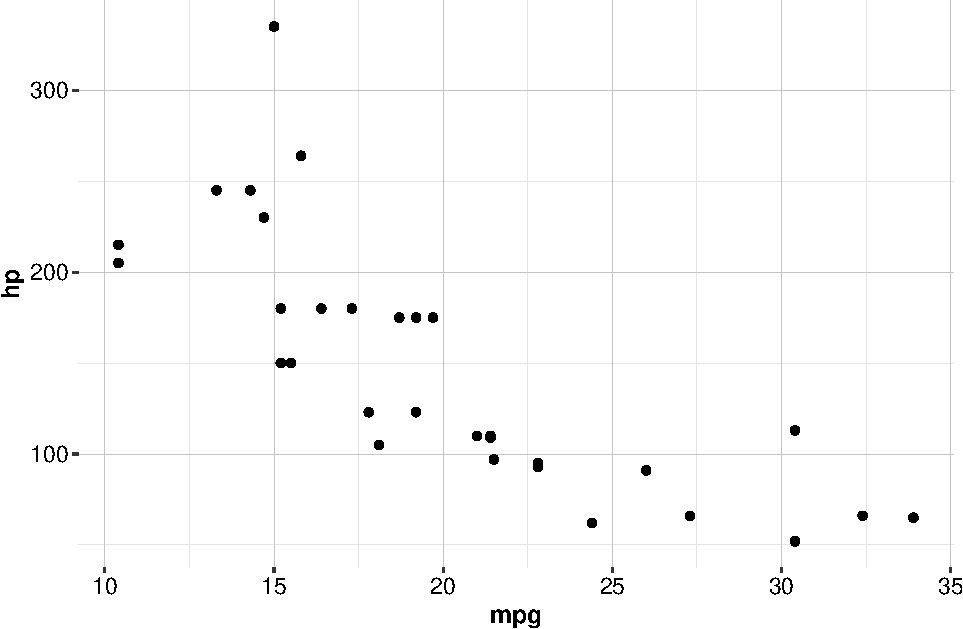
\includegraphics[width=0.7\linewidth]{Intro-R_files/figure-latex/unnamed-chunk-32-1} \end{center}

This code initializes the plot with the \passthrough{\lstinline!ggplot()!} function, specifying the dataset (\passthrough{\lstinline!mtcars!}). The \passthrough{\lstinline!geom\_point()!} function adds points to the plot, and the \passthrough{\lstinline!aes()!} function maps \passthrough{\lstinline!mpg!} to the x-axis and \passthrough{\lstinline!hp!} to the y-axis.

The general template for creating plots with \textbf{ggplot2} follows this structure:

\begin{lstlisting}[language=R]
ggplot(data = <DATA>) +
  <GEOM_FUNCTION>(mapping = aes(<MAPPINGS>))
\end{lstlisting}

Using this template, a variety of visualizations can be created.

\subsection*{Geom Functions in ggplot2}\label{geom-functions-in-ggplot2}
\addcontentsline{toc}{subsection}{Geom Functions in ggplot2}

Geom functions determine the type of plot created in \textbf{ggplot2}. Some commonly used geom functions include:

\begin{itemize}
\tightlist
\item
  \passthrough{\lstinline!geom\_point()!} for scatter plots\\
\item
  \passthrough{\lstinline!geom\_bar()!} for bar plots\\
\item
  \passthrough{\lstinline!geom\_line()!} for line plots\\
\item
  \passthrough{\lstinline!geom\_boxplot()!} for box plots\\
\item
  \passthrough{\lstinline!geom\_histogram()!} for histograms\\
\item
  \passthrough{\lstinline!geom\_density()!} for density plots\\
\item
  \passthrough{\lstinline!geom\_smooth()!} for adding smoothed conditional means to plots
\end{itemize}

For example, to create a smoothed line plot of \passthrough{\lstinline!mpg!} versus \passthrough{\lstinline!hp!}:

\begin{lstlisting}[language=R]
ggplot(data = mtcars) +
  geom_smooth(mapping = aes(x = mpg, y = hp))
\end{lstlisting}

\begin{center}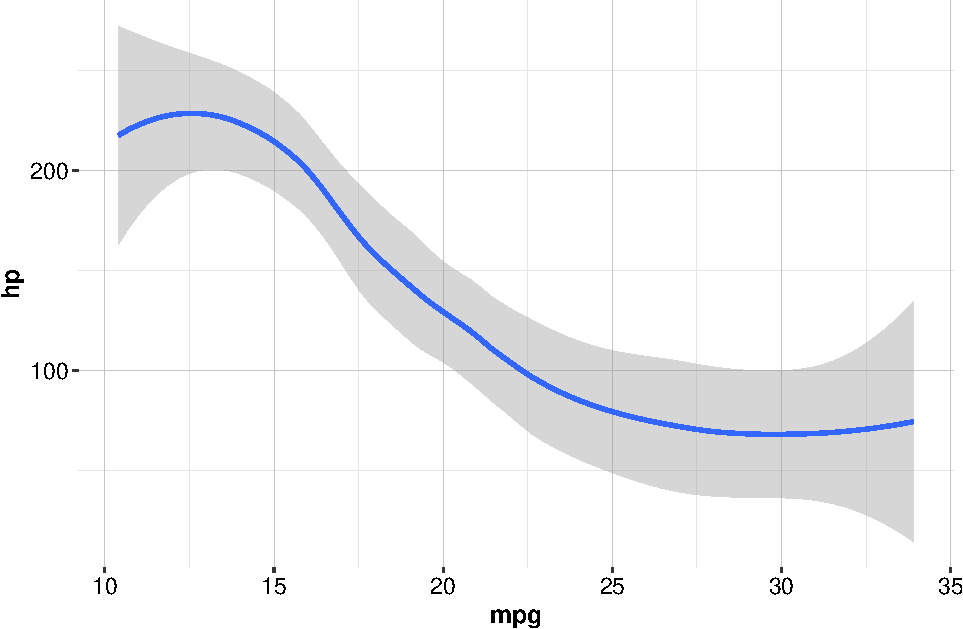
\includegraphics[width=0.7\linewidth]{Intro-R_files/figure-latex/unnamed-chunk-34-1} \end{center}

Multiple geom functions can be combined in a single plot. To overlay a scatter plot on the smoothed line:

\begin{lstlisting}[language=R]
ggplot(data = mtcars) +
  geom_smooth(mapping = aes(x = mpg, y = hp)) + 
  geom_point(mapping = aes(x = mpg, y = hp))
\end{lstlisting}

\begin{center}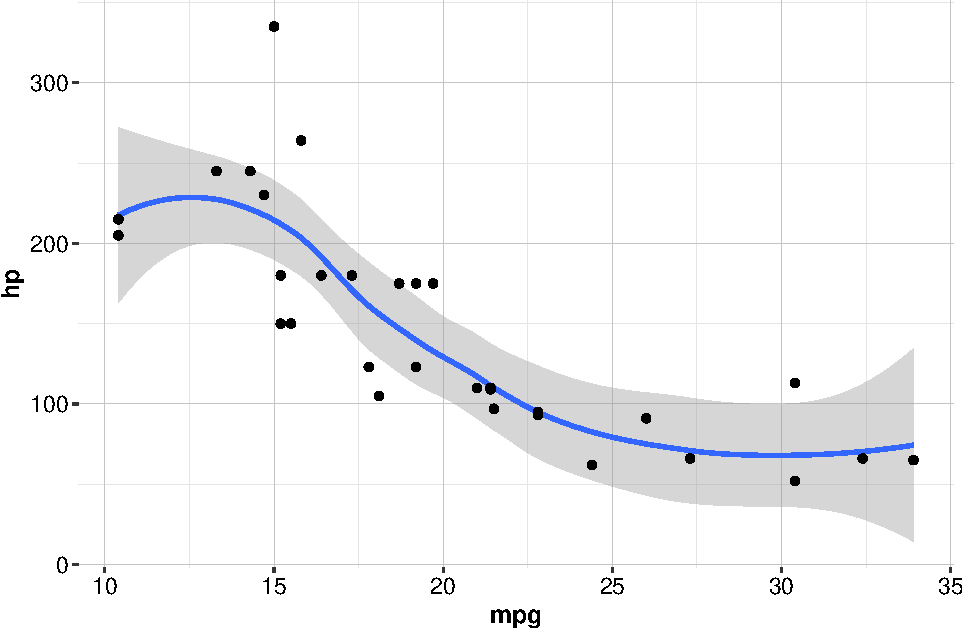
\includegraphics[width=0.7\linewidth]{Intro-R_files/figure-latex/unnamed-chunk-35-1} \end{center}

Alternatively, the \passthrough{\lstinline!aes()!} function can be placed inside \passthrough{\lstinline!ggplot()!} to streamline the code:

\begin{lstlisting}[language=R]
ggplot(data = mtcars, mapping = aes(x = mpg, y = hp)) +
  geom_smooth() + 
  geom_point()
\end{lstlisting}

Additional visualization examples can be found in Chapter \ref{chapter-EDA}. For a complete list of geom functions, refer to the \href{https://ggplot2.tidyverse.org}{\textbf{ggplot2} documentation}.

\subsection*{Aesthetics in ggplot2}\label{aesthetics-in-ggplot2}
\addcontentsline{toc}{subsection}{Aesthetics in ggplot2}

Aesthetics control the visual properties of data points, such as color, size, and shape. These properties are specified within the \passthrough{\lstinline!aes()!} function. For example:

\begin{lstlisting}[language=R]
ggplot(data = mtcars) +
  geom_point(mapping = aes(x = mpg, y = hp, color = cyl))
\end{lstlisting}

\begin{center}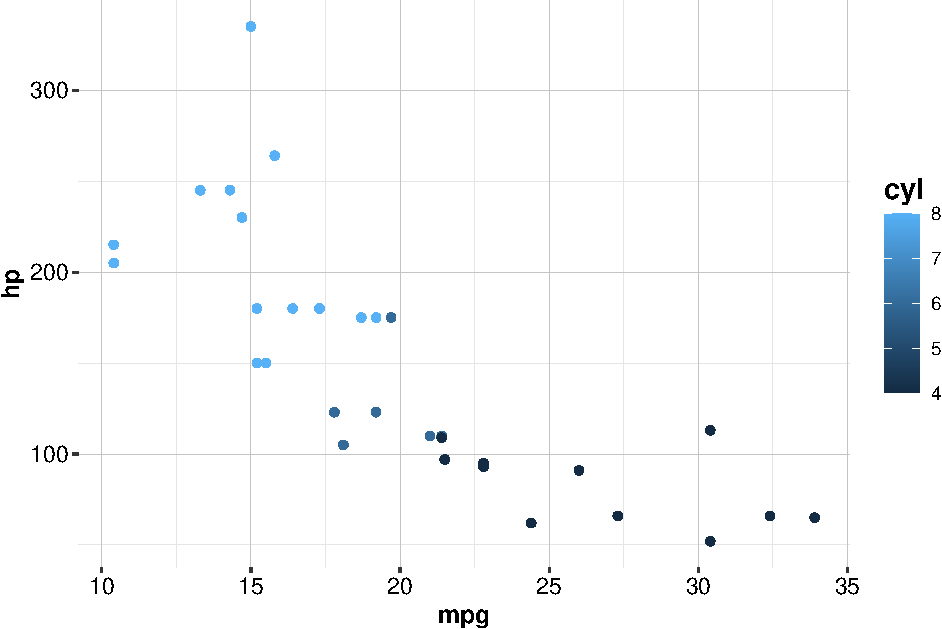
\includegraphics[width=0.7\linewidth]{Intro-R_files/figure-latex/unnamed-chunk-37-1} \end{center}

Here, \passthrough{\lstinline!color = cyl!} maps the color of the points to the number of cylinders (\passthrough{\lstinline!cyl!}) in the \textbf{mtcars} dataset. \textbf{ggplot2} automatically assigns a unique color to each category and adds a corresponding legend.

In addition to \passthrough{\lstinline!color!}, other aesthetics such as \passthrough{\lstinline!size!} and \passthrough{\lstinline!alpha!} (transparency) can be used:

\begin{lstlisting}[language=R]
# Left plot: using the size aesthetic
ggplot(data = mtcars) +
  geom_point(mapping = aes(x = mpg, y = hp, size = cyl))

# Right plot: using the alpha aesthetic
ggplot(data = mtcars) +
  geom_point(mapping = aes(x = mpg, y = hp, alpha = cyl))
\end{lstlisting}

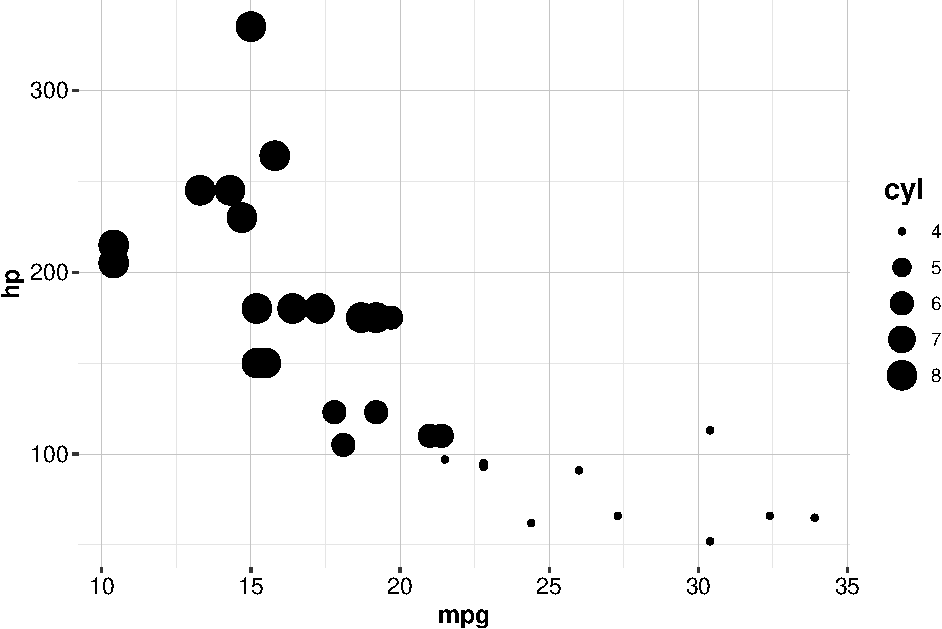
\includegraphics[width=0.5\linewidth]{Intro-R_files/figure-latex/unnamed-chunk-38-1} 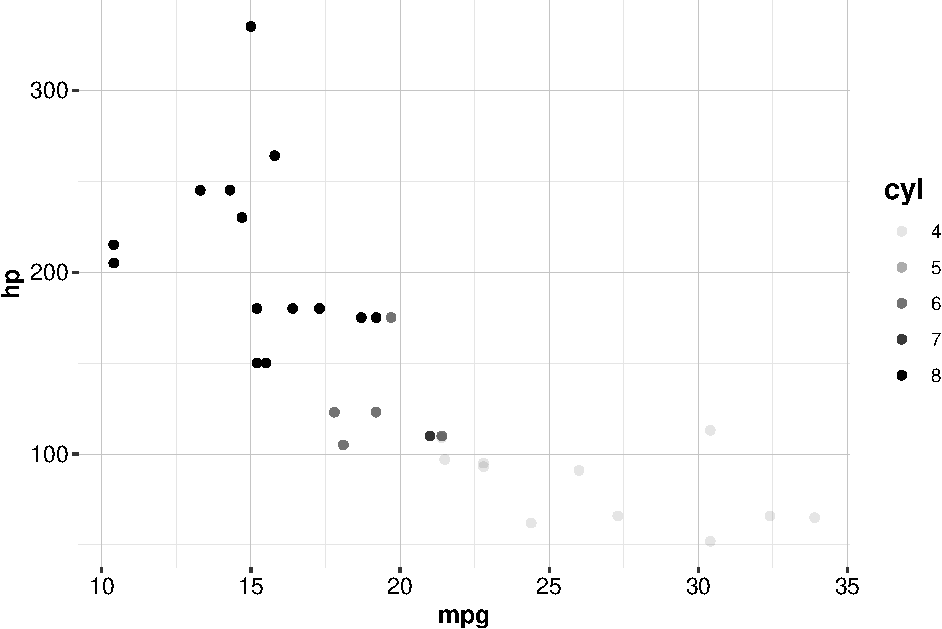
\includegraphics[width=0.5\linewidth]{Intro-R_files/figure-latex/unnamed-chunk-38-2}

Aesthetics can also be set directly inside geom functions. For example, to make all points blue triangles of size 3:

\begin{lstlisting}[language=R]
ggplot(data = mtcars) +
  geom_point(mapping = aes(x = mpg, y = hp), 
             color = "blue", size = 3, shape = 2)
\end{lstlisting}

\begin{center}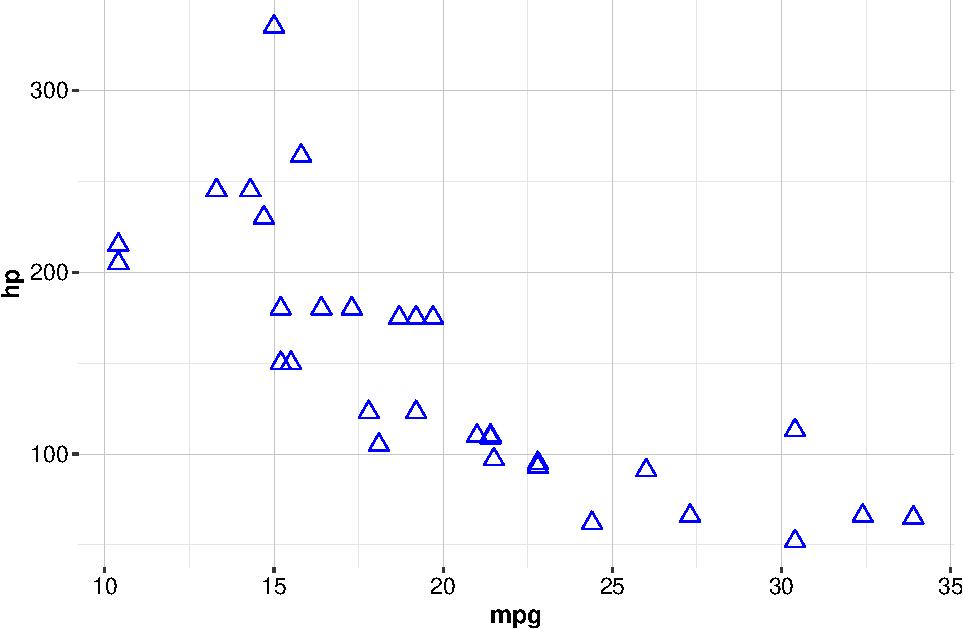
\includegraphics[width=0.7\linewidth]{Intro-R_files/figure-latex/unnamed-chunk-39-1} \end{center}

This section introduced the fundamentals of data visualization in R using \textbf{ggplot2}. The next chapters will explore how visualization plays a crucial role in exploratory data analysis (Chapter \ref{chapter-EDA}) and how to refine plots for communication and reporting. For more details on visualization techniques, see the \href{https://ggplot2.tidyverse.org}{\textbf{ggplot2} documentation}. For interactive graphics, consider exploring the \textbf{plotly} package or \textbf{Shiny} for web applications.

\section{Formula in R}\label{sec-formula-in-R}

Formulas in R provide a concise and intuitive way to specify relationships between variables for statistical modeling. They are widely used in functions for regression, classification, and machine learning to define how a response variable depends on one or more predictors.

In R, formulas use the tilde symbol \passthrough{\lstinline!\~!} to express relationships between variables, where the response variable appears on the left-hand side and predictor variables on the right-hand side. For example, the formula \passthrough{\lstinline!y \~ x!} specifies that \passthrough{\lstinline!y!} is modeled as a function of \passthrough{\lstinline!x!}. When there are multiple predictors, they are separated by \passthrough{\lstinline!+!}.\\
For instance, using the \passthrough{\lstinline!diamonds!} dataset, the formula:

\begin{lstlisting}[language=R]
price ~ carat + cut + color
\end{lstlisting}

models the \passthrough{\lstinline!price!} of a diamond based on its \passthrough{\lstinline!carat!}, \passthrough{\lstinline!cut!}, and \passthrough{\lstinline!color!}.

To include all other variables in the dataset as predictors, we can use the shorthand notation:

\begin{lstlisting}[language=R]
price ~ .
\end{lstlisting}

This approach is particularly useful in large datasets where listing all predictors manually would be impractical.

A formula in R acts as a \textbf{quoting operator}, instructing R to interpret the variables symbolically rather than evaluating them immediately. The variable on the left-hand side of \passthrough{\lstinline!\~!} is the \textbf{dependent variable} (or response variable), while the variables on the right-hand side are the \textbf{independent variables} (or predictor variables).

\begin{example}
\protect\hypertarget{exm:ex-formula}{}\label{exm:ex-formula}To illustrate, suppose we want to predict the \passthrough{\lstinline!price!} of a diamond using a linear regression model. We can pass the formula into the \passthrough{\lstinline!lm()!} function:

\begin{lstlisting}[language=R]
model <- lm(price ~ carat + cut + color, data = diamonds)
\end{lstlisting}

Here, the formula \passthrough{\lstinline!price \~ carat + cut + color!} defines the relationship, and the \passthrough{\lstinline!data!} argument specifies the dataset to use.
\end{example}

Once defined, formulas can be used in various R functions for statistical modeling and machine learning. As you progress through later chapters, you will encounter formulas in functions for regression, classification, and more (e.g., Chapters \ref{chapter-knn}, \ref{chapter-bayes}, and \ref{chapter-regression}). Mastering formula syntax will enable you to efficiently build, customize, and interpret models throughout this book.

\section{Reporting with R Markdown}\label{reporting-with-r-markdown}

Thus far, this book has covered how to interact with R and RStudio for data analysis. This section focuses on an equally important aspect: effectively communicating analytical findings. Data scientists must present results clearly to teams, stakeholders, and clients. Regardless of the depth of an analysis, its impact is limited if it is not communicated effectively. R Markdown facilitates this process by enabling the seamless integration of code, text, and output into dynamic, reproducible reports.

R Markdown allows users to write and execute R code within a document, producing reports, presentations, and dashboards. Unlike traditional notebooks or word processors, R Markdown ensures that text, code, and results remain synchronized as data changes. This book itself is entirely written using R Markdown and generated with the \href{https://bookdown.org}{\textbf{bookdown}} package, ensuring a fully reproducible and dynamic workflow.

R Markdown documents can be exported into multiple formats, including HTML, PDF, Word, and PowerPoint, making it adaptable to various audiences and reporting needs. Furthermore, it supports the creation of interactive documents using Shiny, allowing users to build web applications that facilitate exploratory data analysis.

To get started, the following resources provide useful references:

\begin{itemize}
\tightlist
\item
  \textbf{R Markdown Cheat Sheet}: The \href{https://rstudio.com/wp-content/uploads/2016/03/rmarkdown-cheatsheet-2.0.pdf}{R Markdown Cheat Sheet} offers a concise reference for creating documents, including syntax, formatting, and output options. It is available in RStudio under \emph{Help \textgreater{} Cheatsheets \textgreater{} R Markdown Cheat Sheet}.\\
\item
  \textbf{R Markdown Reference Guide}: The \href{https://rstudio.com/wp-content/uploads/2015/03/rmarkdown-reference.pdf}{R Markdown Reference Guide} provides a detailed overview of R Markdown's features, including document structure and customization.
\end{itemize}

\subsection*{R Markdown Basics}\label{r-markdown-basics}
\addcontentsline{toc}{subsection}{R Markdown Basics}

R Markdown follows a literate programming approach, combining text and executable code in a single document. Unlike word processors where formatting is visible during writing, R Markdown requires compilation to generate the final report. This approach ensures automation, as plots and figures are generated dynamically and inserted into the document. Since the code is embedded, analyses are fully reproducible.

To create an R Markdown document in RStudio:

File \textgreater{} New File \textgreater{} R Markdown

A dialog box will appear, allowing the selection of a document type. For a standard report, choose ``Document.'' Other options include ``Presentation'' for slides, ``Shiny'' for interactive applications, and ``From Template'' for predefined formats. After selecting the document type, enter a title and author name. The output format can be set to HTML, PDF, or Word; HTML is often recommended for debugging.

R Markdown files use the \passthrough{\lstinline!.Rmd!} extension, distinguishing them from \passthrough{\lstinline!.R!} script files. A newly created file contains a template that can be modified with custom text, code, and formatting.

\subsection*{The Header}\label{the-header}
\addcontentsline{toc}{subsection}{The Header}

The header defines metadata such as the document's title, author, date, and output format. It is enclosed within three dashes (\passthrough{\lstinline!---!}).

\begin{lstlisting}
---
title: "An Analysis of Customer Churn"
author: "Reza Mohammadi"
date: "Aug 12, 2024"
output: html_document
---
\end{lstlisting}

\begin{itemize}
\tightlist
\item
  \textbf{Title}: The document's title.\\
\item
  \textbf{Author}: The name of the author.\\
\item
  \textbf{Date}: The date of creation.\\
\item
  \textbf{Output format}: The format of the final document (\passthrough{\lstinline!html\_document!}, \passthrough{\lstinline!pdf\_document!}, or \passthrough{\lstinline!word\_document!}).
\end{itemize}

Additional metadata can be included for customization, such as table of contents options and formatting preferences.

\subsection*{Code Chunks and Inline Code}\label{code-chunks-and-inline-code}
\addcontentsline{toc}{subsection}{Code Chunks and Inline Code}

R Markdown integrates R code within documents using code chunks, which are enclosed in triple backticks (\passthrough{\lstinline!```\{r\}!}) followed by the code. For example:

\begin{lstlisting}

```r
2 + 3
   [1] 5
```
\end{lstlisting}

When compiled, R executes the code and displays the output within the document. Code chunks are used for analysis, visualizations, and modeling. The ``Run'' button in RStudio allows individual execution of chunks. See Figure \ref{fig:run-chunk} for a visual guide.

\begin{figure}

{\centering 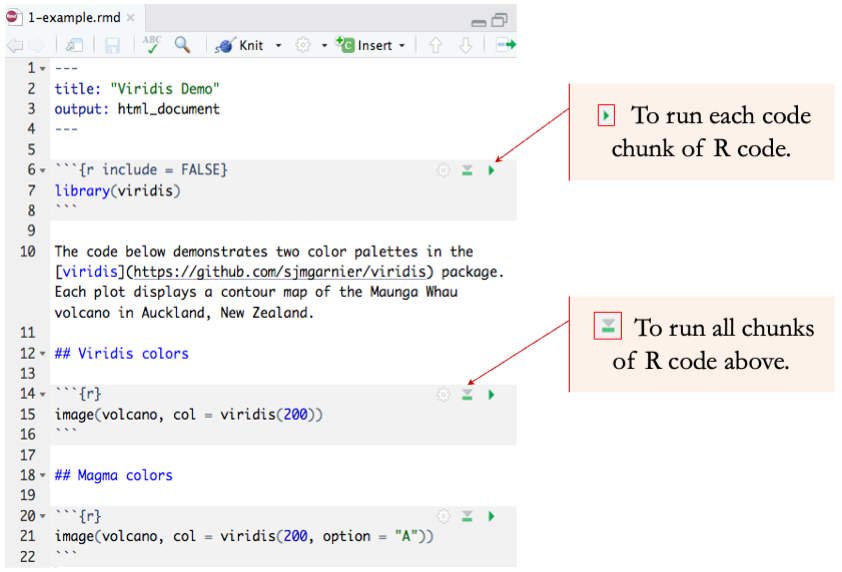
\includegraphics[width=0.9\linewidth]{images/run-chunk} 

}

\caption{Executing a code chunk in R Markdown using the 'Run' button in RStudio.}\label{fig:run-chunk}
\end{figure}

Common chunk options include:

\begin{itemize}
\tightlist
\item
  \passthrough{\lstinline!echo = FALSE!}: Displays output but hides the code.\\
\item
  \passthrough{\lstinline!eval = FALSE!}: Shows the code but does not execute it.\\
\item
  \passthrough{\lstinline!message = FALSE!}: Suppresses messages.\\
\item
  \passthrough{\lstinline!warning = FALSE!}: Suppresses warnings.\\
\item
  \passthrough{\lstinline!error = FALSE!}: Hides error messages.\\
\item
  \passthrough{\lstinline!include = FALSE!}: Omits both code and output.
\end{itemize}

For inline calculations, use backticks and the \passthrough{\lstinline!r!} keyword:

\begin{lstlisting}
The factorial of 5 is 120.
\end{lstlisting}

This renders dynamically as:

\begin{lstlisting}
The factorial of 5 is 120.
\end{lstlisting}

\subsection*{Styling Text}\label{styling-text}
\addcontentsline{toc}{subsection}{Styling Text}

R Markdown supports various text formatting options:

\begin{itemize}
\tightlist
\item
  \textbf{Headings}: Use \passthrough{\lstinline!\#!} for section titles.\\
\item
  \textbf{Bold}: Enclose text in double asterisks (\passthrough{\lstinline!**bold**!}).\\
\item
  \textbf{Italic}: Use single asterisks (\passthrough{\lstinline!*italic*!}).\\
\item
  \textbf{Lists}: Use \passthrough{\lstinline!*!} for bullet points.\\
\item
  \textbf{Links}: \passthrough{\lstinline![R Markdown website](https://rmarkdown.rstudio.com)!}\\
\item
  \textbf{Images}: \passthrough{\lstinline"![Alt text](path/to/image.png)"}
\end{itemize}

For mathematical notation, use LaTeX-style equations:

\begin{lstlisting}
Inline: $y = \beta_0 + \beta_1 x$  
Block: $$ y = \beta_0 + \beta_1 x $$
\end{lstlisting}

\subsection*{Mastering R Markdown}\label{mastering-r-markdown}
\addcontentsline{toc}{subsection}{Mastering R Markdown}

For further learning:

\begin{itemize}
\tightlist
\item
  \textbf{Books}: \href{https://bookdown.org/yihui/rmarkdown/}{\emph{R Markdown: The Definitive Guide}}.\\
\item
  \textbf{Tutorials}: \href{https://rmarkdown.rstudio.com/lesson-1.html}{R Markdown website}.\\
\item
  \textbf{Courses}: \href{https://www.datacamp.com/courses/reporting-with-r-markdown}{DataCamp R Markdown course}.\\
\item
  \textbf{Forums}: \href{https://community.rstudio.com/c/rmarkdown/9}{RStudio Community}.
\end{itemize}

By leveraging R Markdown, data scientists can produce high-quality, reproducible reports that enhance collaboration and communication.

\section{Exercises}\label{intro-R-exercises}

This section provides hands-on exercises to reinforce your understanding of the fundamental concepts covered in this chapter.

\subsection*{Basic Exercises}\label{basic-exercises}
\addcontentsline{toc}{subsection}{Basic Exercises}

\begin{enumerate}
\def\labelenumi{\arabic{enumi}.}
\tightlist
\item
  Install \textbf{R} and \textbf{RStudio} on your computer.\\
\item
  Use the \passthrough{\lstinline!getwd()!} function to check your current working directory. Then, change it to a new directory using \passthrough{\lstinline!setwd()!}.\\
\item
  Create a numeric vector named \passthrough{\lstinline!numbers!} containing the values \passthrough{\lstinline!5, 10, 15, 20, 25!}. Then, calculate the mean and standard deviation of the vector.\\
\item
  Create a matrix with 3 rows and 4 columns, filled with numbers from 1 to 12.\\
\item
  Create a data frame containing the following variables:\\
\end{enumerate}

\begin{itemize}
\tightlist
\item
  \passthrough{\lstinline!student\_id!} (integer)\\
\item
  \passthrough{\lstinline!name!} (character)\\
\item
  \passthrough{\lstinline!score!} (numeric)\\
\item
  \passthrough{\lstinline!passed!} (logical, where \passthrough{\lstinline!TRUE!} means the student passed and \passthrough{\lstinline!FALSE!} means they failed)\\
  Print the first few rows of the data frame using \passthrough{\lstinline!head()!}.\\
\end{itemize}

\begin{enumerate}
\def\labelenumi{\arabic{enumi}.}
\setcounter{enumi}{5}
\tightlist
\item
  Install and load the \textbf{liver} and \textbf{ggplot2} packages in R. If you encounter any errors, check your internet connection and ensure CRAN is accessible.\\
\item
  Load the \emph{churn} dataset from the \textbf{liver} package and display the first few rows using the \passthrough{\lstinline!head()!} function.
\item
  Report the data types of the variables in the \emph{churn} dataset using the \passthrough{\lstinline!str()!} function.
\item
  Report the dimensions of the \emph{churn} dataset using the \passthrough{\lstinline!dim()!} function.
\item
  Report the summary statistics of the variables in the \emph{churn} dataset using the \passthrough{\lstinline!summary()!} function.
\item
  Create a scatter plot using \textbf{ggplot2} that visualizes the relationship between \passthrough{\lstinline!day.mins!} and \passthrough{\lstinline!eve.mins!} in the \emph{churn} dataset. \textbf{Hint:} See the code in Section \ref{EDA-sec-multivariate}.
\item
  Create a histogram for the \passthrough{\lstinline!day.calls!} variable in the \emph{churn} dataset.
\item
  Create a boxplot for the \passthrough{\lstinline!day.mins!} variable in the \emph{churn} dataset.
\item
  Create a boxplot for the \passthrough{\lstinline!day.mins!} variable in the \emph{churn} dataset, grouped by the \passthrough{\lstinline!churn!} variable. \textbf{Hint:} See the code in Section \ref{EDA-sec-numeric}.
\item
  Use the \passthrough{\lstinline!mean()!} function to compute the mean of the \passthrough{\lstinline!customer.calls!} variable in the \emph{churn} dataset. Then, calculate the mean of \passthrough{\lstinline!customer.calls!} for churner \passthrough{\lstinline!churn == yes!}.\\
\item
  Create an R Markdown document that includes a title, author, and a small analysis of the \emph{churn} dataset. Generate an HTML report.
\end{enumerate}

\subsection*{More Challenges Exercise}\label{more-challenges-exercise}
\addcontentsline{toc}{subsection}{More Challenges Exercise}

\begin{enumerate}
\def\labelenumi{\arabic{enumi}.}
\setcounter{enumi}{16}
\tightlist
\item
  The following R code generates a simulated dataset with 200 observations. We will use this simulated dataset as a simple toy example in Chapter \ref{chapter-knn} to explain how k-nearest neighbors algorithm works. This simulated data is for patients with three variables:
\end{enumerate}

\begin{itemize}
\tightlist
\item
  \passthrough{\lstinline!Age!}: Age of the patients as numeric variable with range from 15 to 75 years old.\\
\item
  \passthrough{\lstinline!Ratio!}: Sodium/Potassium ratio in the patient's blood as numeric variable. The ratio is generated based on the \passthrough{\lstinline!Type!} variable.
\item
  \passthrough{\lstinline!Type!}: a factor with three levels: \passthrough{\lstinline!"A"!}, \passthrough{\lstinline!"B"!}, \passthrough{\lstinline!"C"!} representing the type of drug the patient is taking.
\end{itemize}

Run the code and report the summary statistics of the data.

\begin{lstlisting}[language=R]
# Simulate data for kNN
set.seed(10)

n  = 200         # Number of patients
n1 = 90          # Number of patients with drug A
n2 = 60          # Number of patients with drug B 
n3 = n - n1 - n2 # Number of patients with drug C

# Generate Age variable between 15 and 75
Age = sample(x = 15:75, size = n, replace = TRUE)

# Generate Drug Type variable with three levels
Type = sample(x = c("A", "B", "C"), size = n, replace = TRUE, prob = c(n1, n2, n3))

# Generate Sodium/Potassium Ratio based on Drug Type
Ratio = numeric(n)

Ratio[Type == "A"] = sample(x = 10:40, size = sum(Type == "A"), replace = TRUE)
Ratio[Type == "B"] = sample(x =  5:15, size = sum(Type == "B"), replace = TRUE)
Ratio[Type == "C"] = sample(x =  5:15, size = sum(Type == "C"), replace = TRUE)

# Create a data frame with the generated variables
drug_data = data.frame(Age = Age, Ratio = Ratio, Type = Type)
\end{lstlisting}

Visualize the data using the following \textbf{ggplot2} code:

\begin{lstlisting}[language=R]
ggplot(data = drug_data, aes(x = Age, y = Ratio)) +
  geom_point(aes(color = Type, shape = Type)) + 
  labs(title = "Age vs. Sodium/Potassium Ratio", 
       x = "Age", y = "Sodium/Potassium Ratio")
\end{lstlisting}

\begin{center}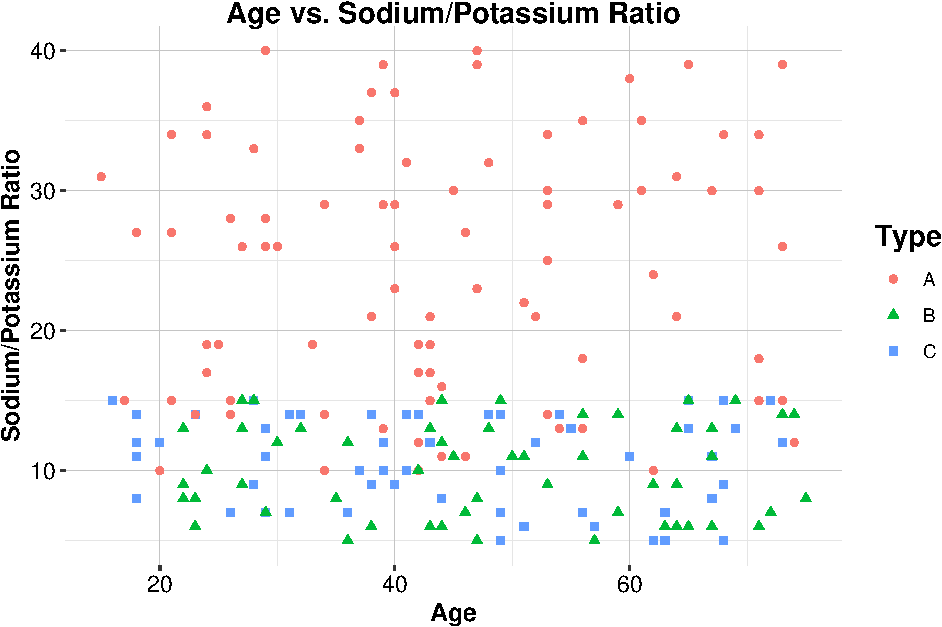
\includegraphics[width=0.7\linewidth]{Intro-R_files/figure-latex/unnamed-chunk-45-1} \end{center}

\begin{enumerate}
\def\labelenumi{\arabic{enumi}.}
\setcounter{enumi}{17}
\tightlist
\item
  Extend the dataset \passthrough{\lstinline!drug\_data!} by adding a new variable named \passthrough{\lstinline!Outcome!}, which is a factor with two levels (\passthrough{\lstinline!"Good"!} and \passthrough{\lstinline!"Bad"!}).\\
\end{enumerate}

\begin{itemize}
\tightlist
\item
  Patients with \passthrough{\lstinline!Type == "A"!} should have a higher probability of \passthrough{\lstinline!"Good"!} outcomes.\\
\item
  Patients with \passthrough{\lstinline!Type == "B"!} and \passthrough{\lstinline!Type == "C"!} should have a lower probability of \passthrough{\lstinline!"Good"!} outcomes.\\
\item
  Use \passthrough{\lstinline!sample()!} with appropriate probabilities to generate the \passthrough{\lstinline!Outcome!} variable.\\
\end{itemize}

\begin{enumerate}
\def\labelenumi{\arabic{enumi}.}
\setcounter{enumi}{18}
\tightlist
\item
  Create a new scatter plot using \textbf{ggplot2} that visualizes the relationship between \passthrough{\lstinline!Age!} and \passthrough{\lstinline!Ratio!}, colored by the \passthrough{\lstinline!Outcome!} variable.
\item
  Create a new variable \passthrough{\lstinline!Age\_group!} in the \passthrough{\lstinline!drug\_data!} dataset that categorizes patients into three groups:\\
\end{enumerate}

\begin{itemize}
\tightlist
\item
  ``Young'' (\(\leq 30\) years old)
\item
  ``Middle-aged'' (31-50 years old)
\item
  ``Senior'' (\textgreater50 years old).
\end{itemize}

\begin{enumerate}
\def\labelenumi{\arabic{enumi}.}
\setcounter{enumi}{20}
\tightlist
\item
  Calculate the mean \passthrough{\lstinline!Ratio!} for each \passthrough{\lstinline!Age\_group!} category in the \passthrough{\lstinline!drug\_data!} dataset.\\
\item
  Create a bar chart using \textbf{ggplot2} that displays the average \passthrough{\lstinline!Ratio!} for each \passthrough{\lstinline!Age\_group!}.\\
\item
  Modify the \passthrough{\lstinline!drug\_data!} dataset by adding a \passthrough{\lstinline!Risk\_factor!} variable, calculated as \passthrough{\lstinline!Ratio * Age / 10!}. Analyze how \passthrough{\lstinline!Risk\_factor!} differs by \passthrough{\lstinline!Type!}.\\
\item
  Create a histogram of the \passthrough{\lstinline!Risk\_factor!} variable, grouped by \passthrough{\lstinline!Type!}.\\
\item
  Generate a boxplot to visualize the distribution of \passthrough{\lstinline!Risk\_factor!} across different \passthrough{\lstinline!Outcome!} categories.
\end{enumerate}

\chapter{Introduction to Data Science}\label{chapter-intro-DS}

\emph{Data Science} is a rapidly evolving field that is transforming industries by leveraging computational, statistical, and analytical techniques. In the 21st century, data has become one of the most valuable resources, often called the \emph{``new oil''} due to its potential to drive innovation and reshape the future.

Data science is the key to unlocking this potential. By applying computational, statistical, and analytical techniques, data scientists extract insights from vast amounts of data, enabling organizations to make informed decisions, optimize processes, predict trends, and develop intelligent systems. This has led to groundbreaking advancements in fields such as healthcare, finance, marketing, artificial intelligence (AI), and beyond.

Given its rapid growth and increasing demand, data science is more critical than ever. In this chapter, we'll explore the fundamentals of data science, discuss its significance in modern society, and introduce the Data Science Workflow---a structured approach that data scientists use to transform raw data into actionable insights.

This section is well-structured and provides a clear introduction to data science. It effectively conveys the interdisciplinary nature of the field and highlights its core components. However, there are some areas where clarity, consistency, and flow can be improved. Below are my suggestions:

\section{What is Data Science?}\label{what-is-data-science}

Data science is an interdisciplinary field that integrates computer science, statistics, and domain expertise to extract insights from data. It involves using analytical and computational techniques to process vast amounts of raw data, transforming them into meaningful information that supports decision-making and strategic planning.

\begin{figure}

{\centering 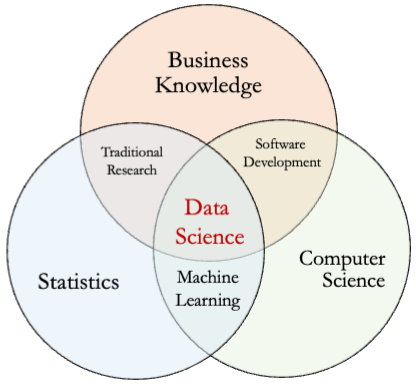
\includegraphics[width=0.5\linewidth]{images/data_science} 

}

\caption{Data science is a multidisciplinary field that applies computational and statistical methods to extract insights from data.}\label{fig:Data-Science}
\end{figure}

Although the term ``data science'' is relatively new, its foundations lie in well-established disciplines such as statistics, data analysis, and machine learning. With the exponential growth of digital data, advancements in computational power, and the increasing demand for data-driven decision-making, data science has emerged as a distinct and essential field.

At its core, data science is concerned with extracting knowledge from data using a combination of statistical techniques, machine learning algorithms, and domain-specific methodologies. It helps organizations manage and understand the vast amounts of information generated in the digital age.

\subsection*{Key Components of Data Science}\label{key-components-of-data-science}
\addcontentsline{toc}{subsection}{Key Components of Data Science}

The field of data science encompasses three main components:

\begin{itemize}
\tightlist
\item
  \textbf{Data Engineering}: The foundation of data science, responsible for collecting, storing, and structuring large datasets. This includes the development of data pipelines and infrastructure to enable efficient analysis. While crucial, data engineering is beyond the scope of this book.\\
\item
  \textbf{Data Analysis and Statistics}: The application of statistical methods to explore and analyze data. This includes data visualization, hypothesis testing, and predictive modeling. More details on this topic are covered in the \hyperref[chapter-statistics]{Statistical Inference and Hypothesis Testing} and \hyperref[chapter-EDA]{Exploratory Data Analysis} chapters.\\
\item
  \textbf{Machine Learning and Artificial Intelligence}: The use of algorithms to identify patterns, make predictions, and extract deeper insights. This includes supervised and unsupervised learning, deep learning, and natural language processing. These concepts are discussed in the \hyperref[chapter-modeling]{Modeling Process} chapter.
\end{itemize}

\section{Why Data Science Matters}\label{why-data-science-matters}

In the digital age, data has become one of the most valuable resources and is often referred to as the ``new oil'' of the 21st century. This comparison makes sense, as some of the world's most valuable companies today---including OpenAI, Google, and Apple---are driven by artificial intelligence and data science. Just as the wealthiest companies of the 20th century were those that controlled oil and energy, today's leading enterprises leverage data as a key asset for innovation and competitive advantage.

Across industries, data-driven decision-making has become essential. Organizations generate vast amounts of data every day, and without the right tools and techniques, much of this data would remain untapped. Data science helps organizations uncover patterns, detect trends, and make informed decisions that enhance efficiency, reduce costs, and improve customer experiences.\\
Data science plays a crucial role in a wide range of sectors, including:

\begin{itemize}
\tightlist
\item
  \emph{Finance}: Financial institutions leverage data science for risk assessment, fraud detection, and algorithmic trading. Machine learning models identify anomalies in transaction patterns, improving fraud detection and regulatory compliance.\\
\item
  \emph{Marketing}: Businesses use data science to analyze customer behavior, segment audiences, and create targeted marketing campaigns. Platforms such as Facebook and Google Ads leverage sophisticated algorithms to match advertisements with the most relevant audiences, improving engagement and conversion rates.\\
\item
  \emph{Retail and E-commerce}: Companies like Amazon and Walmart use data science to optimize inventory management, predict demand, and personalize recommendations. By analyzing purchase history and browsing behavior, retailers can offer tailored promotions and enhance customer satisfaction.\\
\item
  \emph{Healthcare}: Hospitals and medical researchers use data science for disease diagnosis, patient risk prediction, and personalized treatment plans. By analyzing large datasets of medical records, institutions can identify high-risk patients and take preventative measures to improve health outcomes.
\end{itemize}

For example, Netflix applies data science to analyze viewing patterns and recommend personalized content to users, while supply chain optimization at Amazon ensures faster deliveries by leveraging predictive analytics.

\section{The Data Science Workflow}\label{the-data-science-workflow}

The \emph{data science workflow} follows an \emph{iterative} and \emph{cyclical} approach, where insights gained at each stage inform and refine subsequent steps. Unlike a strictly linear process, data science involves continuous refinement to enhance accuracy and efficiency. This structured approach ensures that data-driven projects are conducted systematically, balancing exploratory analysis, model building, and evaluation to derive meaningful conclusions.

A \emph{data science workflow} follows a phased, adaptive approach within a scientific framework, transforming raw data into actionable knowledge. This transformation is often conceptualized using the \emph{DIKW Pyramid} (Data → Information → Knowledge → Wisdom), as illustrated in Figure \ref{fig:DIKW-Pyramid}.

\begin{figure}

{\centering 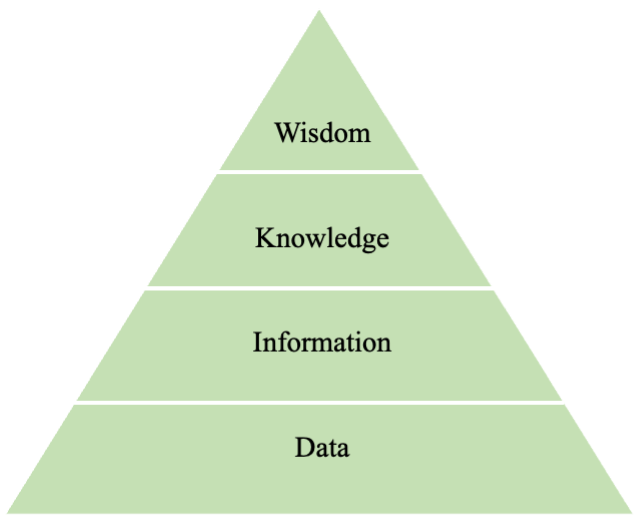
\includegraphics[width=0.4\linewidth]{images/DIKW-Pyramid} 

}

\caption{The DIKW Pyramid illustrates the transformation of raw data into actionable insights, progressing from data to information, knowledge, and ultimately wisdom.}\label{fig:DIKW-Pyramid}
\end{figure}

While the specifics may vary across projects, most data science workflows follow a common structure. In this book, we adopt the \emph{Data Science Workflow} as a guiding framework for structuring data science projects. This workflow is inspired by the \emph{Cross-Industry Standard Process for Data Mining (CRISP-DM)} model, a widely recognized methodology for data-driven projects. It is a \emph{cyclic} framework that guides data scientists through the following key stages (see Figure \ref{fig:CRISP-DM}):

\begin{enumerate}
\def\labelenumi{\arabic{enumi}.}
\tightlist
\item
  \textbf{Problem Understanding} -- Defining the business or research question and outlining objectives.\\
\item
  \textbf{Data Preparation} -- Collecting, cleaning, transforming, and organizing data to ensure it is suitable for analysis. This step includes handling missing values, addressing inconsistencies, detecting outliers, and preparing features through scaling, encoding, and transformation.\\
\item
  \textbf{Exploratory Data Analysis (EDA)} -- Identifying patterns, distributions, and relationships within the data.\\
\item
  \textbf{Preparing Data for Modeling} -- Engineering relevant features, normalizing data, and selecting meaningful variables.\\
\item
  \textbf{Modeling} -- Applying machine learning or statistical techniques to develop predictive or descriptive models.\\
\item
  \textbf{Evaluation} -- Assessing model performance using appropriate metrics and validation techniques.\\
\item
  \textbf{Deployment} -- Integrating the model into a production environment and monitoring its performance over time.
\end{enumerate}

\begin{figure}

{\centering 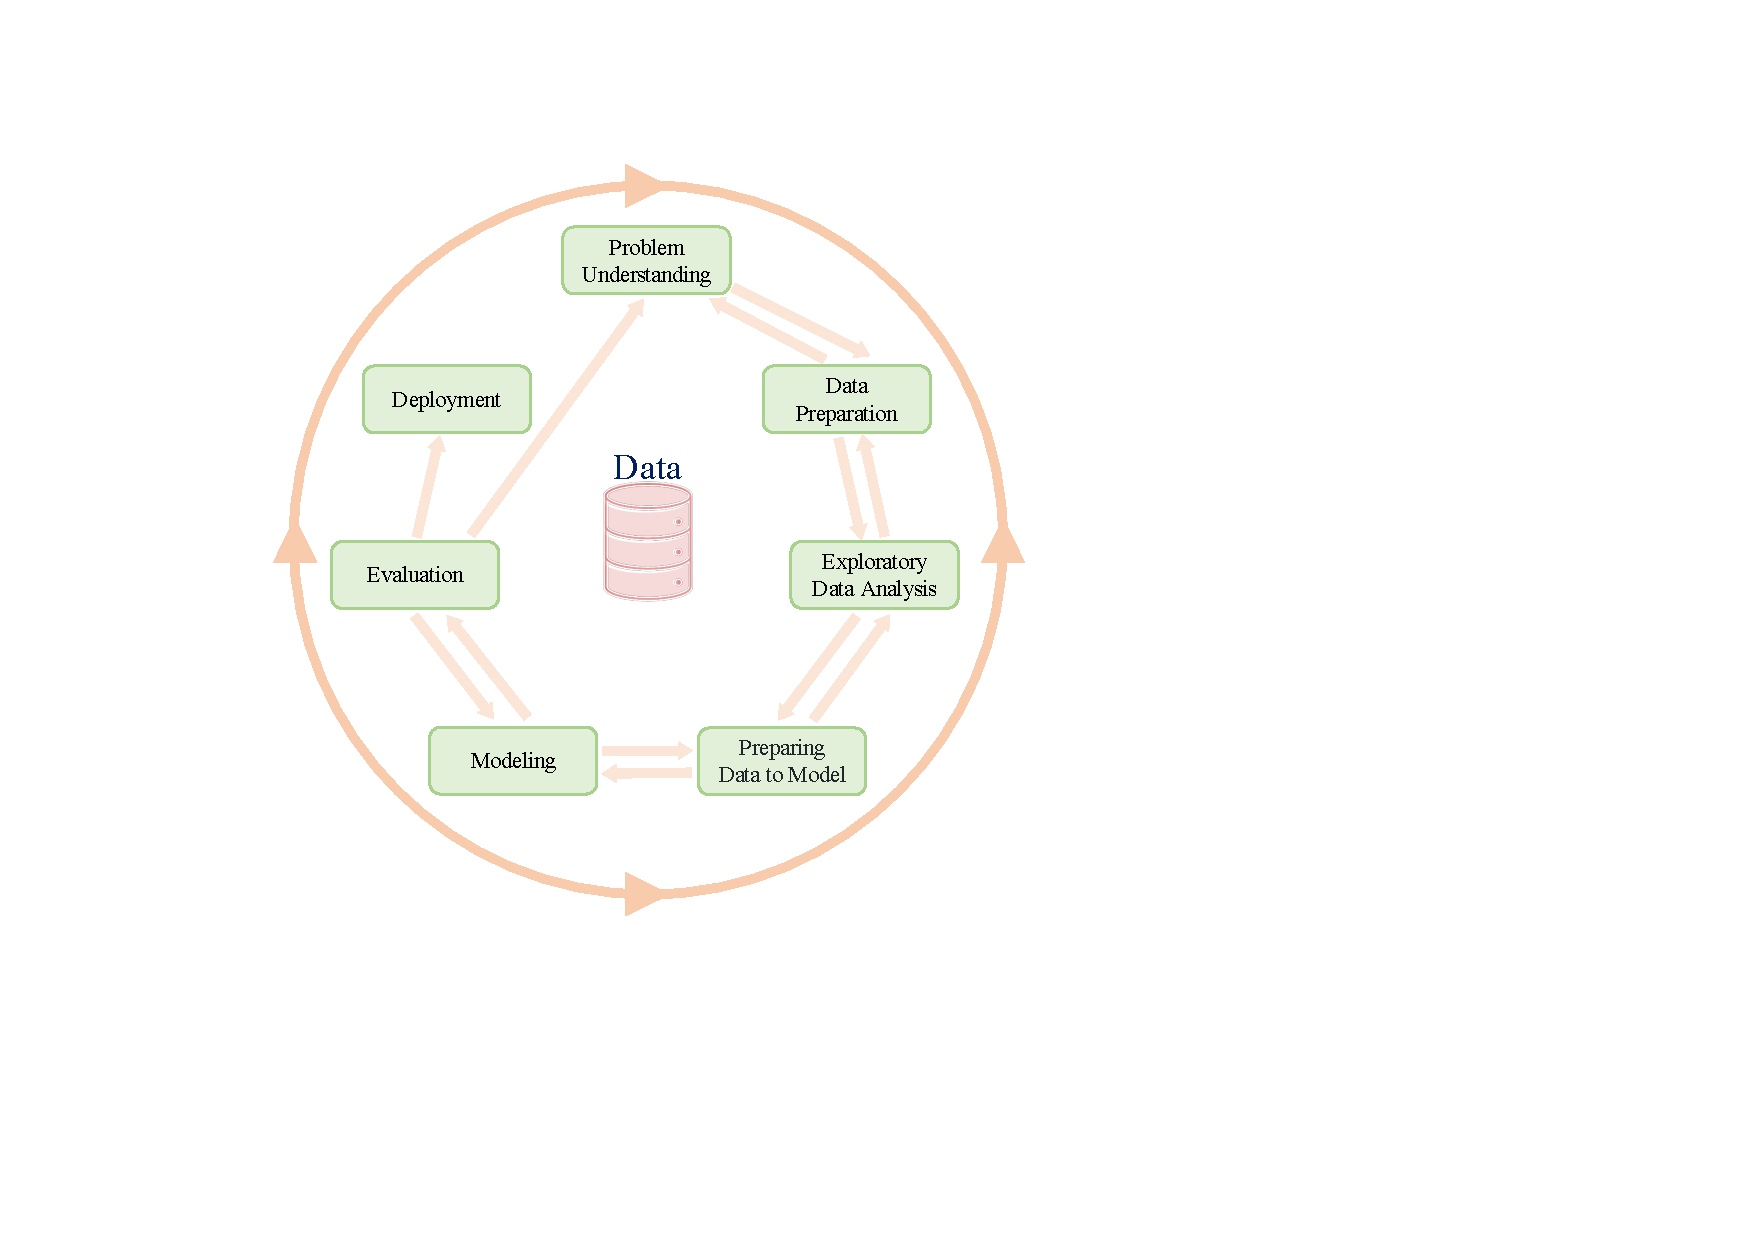
\includegraphics[width=0.6\linewidth]{images/DSW} 

}

\caption{The Data Science Workflow is an iterative framework for structuring data science and machine learning projects. Inspired by the CRISP-DM model, it ensures systematic problem-solving and continuous refinement.}\label{fig:CRISP-DM}
\end{figure}

Because data science is inherently \emph{iterative}, these steps are often revisited multiple times within a single project. The \emph{feedback loops} between stages allow for continuous refinement---adjusting data preprocessing, modifying features, or retraining models as new insights emerge. By following a structured workflow, data scientists can ensure rigor, accuracy, and efficiency in transforming data into valuable insights.

\section{Problem Understanding}\label{problem-understanding}

The first step in any data science project is to clearly define the problem---whether it is a business challenge or a research question. This phase is crucial because data science is not just about building models; it is about solving real-world problems using data-driven approaches. A well-defined problem ensures that efforts are aligned with meaningful objectives, improving the likelihood of delivering actionable insights.

At this stage, data scientists work closely with stakeholders to understand the goals, clarify expectations, and define success criteria. The following questions help frame the problem:

\begin{itemize}
\tightlist
\item
  \textbf{Why} is this research or business question important?\\
\item
  \textbf{What} is the desired outcome or impact?\\
\item
  \textbf{How} can data science techniques contribute to addressing this question?
\end{itemize}

Focusing on the \emph{why} and \emph{what} before diving into the \emph{how} is essential. As Simon Sinek emphasizes in his TED talk \href{https://www.ted.com/talks/simon_sinek_how_great_leaders_inspire_action?utm_campaign=tedspread&utm_medium=referral&utm_source=tedcomshare}{``How Great Leaders Inspire Action''}, ``People don't buy what you do; they buy why you do it.'' This concept applies to data science as well---understanding the deeper motivation behind a project provides clarity and direction.

For example, a data science team in a business analytics department may be approached by a client who wants a predictive model but lacks clarity on the specific problem they are trying to solve. Without a clear \emph{why}, it becomes difficult to develop a solution that delivers real value. Similarly, students working on research projects often focus on \emph{what} they want to build rather than \emph{why} it is needed.

Suppose a company aims to reduce customer churn. A well-defined objective might be to develop a predictive model that identifies customers at risk of leaving so that targeted retention strategies can be implemented. This initial understanding helps frame the problem and guides the selection of relevant data, modeling techniques, and evaluation metrics.

Problem understanding is both an analytical and creative process. While data science provides tools and methodologies, defining the right problem requires domain expertise and critical thinking. The following steps help ensure a structured approach:

\begin{enumerate}
\def\labelenumi{\arabic{enumi}.}
\tightlist
\item
  \textbf{Clearly articulate the project objectives} and requirements in terms of the overall goals of the business or research entity.
\item
  \textbf{Break down the objectives} to outline specific expectations and desired outcomes.
\item
  \textbf{Translate these objectives into a data science problem} that can be addressed using analytical techniques.
\item
  \textbf{Draft a preliminary strategy} for how to achieve these objectives, considering potential approaches and methodologies.
\end{enumerate}

By thoroughly defining the problem, data scientists set the stage for an effective workflow, ensuring that subsequent analysis and modeling efforts remain aligned with meaningful outcomes.

\section{Data Preparation}\label{data-preparation}

Once the problem is well-defined, the next step is \emph{data preparation}, ensuring the data is accurate, complete, and well-structured. Raw data often contains \emph{missing values, inconsistencies, and outliers}, making this phase critical for reliable analysis. Poorly prepared data can lead to misleading insights, even with sophisticated models.

Data can originate from various sources, including databases, spreadsheets, APIs, and web scraping. It may be \emph{structured} (e.g., numerical data in databases) or \emph{unstructured} (e.g., text, images). Preprocessing is essential before analysis.

Key steps in data preparation include:

\begin{itemize}
\tightlist
\item
  \emph{Data Collection and Integration}: Merging data from multiple sources while ensuring consistency.\\
\item
  \emph{Handling Missing Values}: Removing, imputing, or flagging incomplete data.\\
\item
  \emph{Outlier Detection}: Identifying and managing extreme values using visualization.\\
\item
  \emph{Resolving Inconsistencies}: Standardizing formats, correcting errors, and aligning categorical values.\\
\item
  \emph{Feature Engineering}: Transforming data through encoding, scaling, and normalization for model compatibility.\\
\item
  \emph{Data Summarization}: Checking variable types, computing summary statistics, and detecting duplicates.
\end{itemize}

Though time-consuming, data preparation is essential for accurate modeling and meaningful analysis. In Chapter \ref{chapter-data-prep}, we explore these techniques further with real-world examples.

\section{Exploratory Data Analysis (EDA)}\label{exploratory-data-analysis-eda}

Exploratory Data Analysis (EDA) is a fundamental step in the data science workflow, providing an initial understanding of the dataset before formal modeling. The primary objective of EDA is to uncover patterns, relationships, and anomalies in the data, helping data scientists refine hypotheses and validate assumptions. By systematically examining the data, EDA ensures that the subsequent modeling process is informed by a solid understanding of the dataset's structure and characteristics.

Several key techniques are commonly used in EDA:

\begin{itemize}
\tightlist
\item
  \emph{Summary statistics} -- Measures such as the mean, median, standard deviation, and interquartile range provide insights into the distribution and central tendencies of numerical variables.\\
\item
  \emph{Data visualization} -- Graphical techniques, including histograms, scatter plots, and box plots, reveal data distributions, trends, and potential outliers.\\
\item
  \emph{Correlation analysis} -- Examining relationships between numerical features using correlation coefficients helps identify dependencies that may influence modeling decisions.
\end{itemize}

EDA serves both diagnostic and exploratory functions. It helps detect data quality issues, such as missing values or inconsistencies, while also guiding feature selection and engineering. For instance, if a strong correlation exists between certain features and the target variable, these features may be prioritized in the modeling phase.

A thorough EDA process not only improves the quality of the dataset but also enhances the interpretability and reliability of analytical results. In Chapter \ref{chapter-EDA}, we will explore EDA techniques in greater detail, applying them to real-world datasets to illustrate practical applications.

\section{Preparing Data for Modeling}\label{preparing-data-for-modeling}

With insights from EDA, the next step is to \emph{prepare the data for modeling}. This stage involves \emph{feature engineering}, \emph{feature selection}, and \emph{data splitting}---all of which are crucial for building effective models.

\begin{itemize}
\tightlist
\item
  \emph{Feature Engineering}: Creating new features or transforming existing ones to enhance model performance. For example, deriving new variables by combining existing ones or applying transformations can provide additional predictive power.\\
\item
  \emph{Feature Selection}: Identifying and selecting the most relevant features to improve model efficiency and prevent overfitting. Removing irrelevant or redundant features simplifies the model and enhances interpretability.\\
\item
  \emph{Data Splitting}: Dividing the dataset into training, validation, and testing sets. The training set is used to develop the model, the validation set helps fine-tune parameters, and the test set assesses final model performance.
\end{itemize}

By the end of this stage, the data should be in a structured and well-prepared format, ensuring that models can learn effectively. In Chapter \ref{chapter-modeling}, we will explore these techniques in more detail and apply them to real-world datasets.

\section{Modeling}\label{modeling}

Modeling is the stage where data scientists apply machine learning or statistical techniques to the prepared data to create a predictive or descriptive model. The goal is to build a model that effectively captures relationships within the data and generalizes well to new, unseen data.

The modeling process typically involves:

\begin{itemize}
\tightlist
\item
  \emph{Choosing a Model}: Selecting an appropriate model based on the problem type (e.g., regression, classification, clustering) and the characteristics of the dataset.\\
\item
  \emph{Training the Model}: Fitting the model to the training data to learn patterns and relationships.\\
\item
  \emph{Tuning Hyperparameters}: Adjusting model parameters to optimize performance on the validation set.
\end{itemize}

Common algorithms include linear regression (Chapter \ref{chapter-regression}), decision trees (Chapter \ref{chapter-tree}), Naïve Bayes classifier (Chapter \ref{chapter-bayes}), k-Nearest Neighbors (k-NN) algorithm (Chapter \ref{chapter-knn}), and neural networks (Chapter \ref{chapter-nn}). Each method has its strengths and limitations, and selecting the most suitable model depends on the nature of the problem, data quality, and computational constraints. Often, multiple models are tested and compared to determine the best-performing approach.

\section{Evaluation}\label{evaluation}

Once a model is built, it must be rigorously evaluated to ensure its accuracy, generalizability, and robustness before deployment. The evaluation process relies on well-defined performance metrics, which vary depending on the type of problem. For classification models, commonly used metrics include accuracy, precision, recall, F1-score, and the area under the receiver operating characteristic curve (ROC-AUC). In regression tasks, measures such as mean squared error (MSE), mean absolute error (MAE), and the coefficient of determination (\(R^2\)) assess model effectiveness.

To ensure the model is not overfitting to the training data, cross-validation techniques, such as k-fold cross-validation, are employed. These methods provide a more reliable estimate of a model's performance by partitioning the data into multiple subsets for training and validation. Beyond numerical evaluation, error analysis plays a crucial role in diagnosing weaknesses, particularly through confusion matrix interpretation for classification problems and residual analysis for regression. A careful examination of errors often reveals underlying biases, data inconsistencies, or model limitations that require refinement.

If the model fails to meet expectations, adjustments may be necessary, such as feature selection, hyperparameter tuning, or exploring alternative modeling approaches. In Chapter \ref{chapter-evaluation}, we will explore these techniques in detail and apply them to real-world datasets.

\section{Deployment}\label{deployment}

Once the model has been evaluated and meets the project goals, the final step is deployment, where it is integrated into a production environment to generate real-time insights or predictions. This phase is crucial for ensuring that the model contributes tangible value, whether by supporting decision-making processes or by automating tasks within operational systems. Models can be deployed in various ways, such as embedding them in web applications, integrating them into enterprise software, or automating processes in large-scale data pipelines.

Beyond initial integration, continuous monitoring is essential to track the model's performance and detect potential issues. As real-world data evolves, models may experience \emph{concept drift}, where their predictive accuracy deteriorates due to changes in underlying patterns. To mitigate this, periodic model updates and retraining are necessary to maintain reliability. Additionally, implementing robust logging and performance tracking mechanisms helps ensure that discrepancies between predicted and actual outcomes are quickly identified and addressed.

Deployment is not a one-time event but an ongoing process. Effective deployment strategies account for scalability, interpretability, and maintainability, allowing models to remain useful in dynamic environments. As the field of data science advances, the ability to manage deployed models effectively will continue to be a critical factor in transforming analytical insights into real-world impact.

\section{Machine Learning}\label{machine-learning}

Data science relies on machine learning techniques to extract insights from data, make predictions, and uncover patterns. These methods enable data scientists to move beyond descriptive analysis and explore predictive and prescriptive approaches, which are essential for real-world applications. In this section, we provide an overview of machine learning, including its main types---\emph{supervised learning} and \emph{unsupervised learning}---and discuss how machine learning differs from statistical learning.

Machine learning is a branch of artificial intelligence that focuses on developing algorithms that learn from data and make predictions. Rather than being explicitly programmed for each task, machine learning models identify patterns within data and use them to make informed decisions. This approach is particularly useful for complex problems where rule-based programming would be impractical.

For instance, rather than defining a fixed set of rules to detect spam emails, a machine learning model can be trained on a labeled dataset of emails classified as ``spam'' or ``not spam.'' The model learns distinguishing patterns and can classify new emails with high accuracy. This ability to generalize from data makes machine learning invaluable in fields such as finance, healthcare, and marketing.

\subsection*{Machine Learning Tasks: Supervised vs.~Unsupervised Learning}\label{machine-learning-tasks-supervised-vs.-unsupervised-learning}
\addcontentsline{toc}{subsection}{Machine Learning Tasks: Supervised vs.~Unsupervised Learning}

Machine learning tasks can be broadly categorized into \emph{supervised learning} and \emph{unsupervised learning}, which differ in terms of how models learn from data and the objectives of the analysis.

\textbf{Supervised learning} involves training a model on a labeled dataset, where each data point is associated with a known output. The goal is for the model to learn the relationship between input features and the corresponding output, enabling it to make accurate predictions on new data. Common supervised learning tasks include classification and numeric prediction. In classification, the model assigns data points to predefined categories, such as detecting whether an email is spam or identifying whether a patient has a particular disease. This book covers classification techniques such as decision trees (Chapter \ref{chapter-tree}), the Naïve Bayes classifier (Chapter \ref{chapter-bayes}), and the k-Nearest Neighbors (k-NN) algorithm (Chapter \ref{chapter-knn}). Numeric prediction, also known as regression, focuses on estimating continuous values, such as forecasting house prices based on location and size. A detailed discussion of regression techniques is provided in Chapter \ref{chapter-regression}.

\textbf{Unsupervised learning}, on the other hand, is applied to datasets that lack labeled outputs. The objective is to uncover hidden patterns, relationships, or structures within the data. Clustering, a common unsupervised learning technique, groups data points based on similarity, such as segmenting customers according to purchasing behavior. Another important unsupervised learning method is pattern discovery, also known as association rule learning, which identifies relationships between variables. This technique is widely used in market basket analysis to detect frequently co-purchased items. These concepts are explored in further detail in Chapter \ref{chapter-cluster}.

In summary, supervised learning is used when labeled data is available and a specific predictive outcome is required, while unsupervised learning is beneficial for exploratory data analysis, where the goal is to identify underlying structures in unlabeled data. The distinction between these two approaches is fundamental to selecting appropriate machine learning techniques for a given data science problem.

\section{Exercises}\label{exercises}

The following exercises will help reinforce the key concepts covered in this chapter. The questions range from fundamental definitions to applied problem-solving related to data science, the data science workflow, and machine learning.

\begin{enumerate}
\def\labelenumi{\arabic{enumi}.}
\tightlist
\item
  How does data-driven decision-making impact businesses? Give an example of a real-world application.\\
\item
  \emph{Data Science Workflow} is inspired by the \emph{CRISP-DM} model. What does \emph{CRISP-DM} stand for, and how does it guide data-driven projects? What are the key stages of the \emph{CRISP-DM} model?\\
\item
  \emph{Data Science Workflow} and \emph{CRISP-DM} model are not the only standard processes for data science projects. What are some other methodologies used in the industry?\\
\item
  Do you think we can skip the \emph{Problem Understanding} phase and directly jump to \emph{Data Preparation} in a data science project? Justify your answer.\\
\item
  Why is \emph{Data Preparation} considered one of the most time-consuming steps in a data science project? What are some common challenges faced during this phase?\\
\item
  To what extent can Data Science projects be automated without human intervention? What are the risks and limitations of relying solely on automated tools?\\
\item
  For each of the following scenarios, identify the appropriate stage in the data science workflow:

  \begin{enumerate}
  \def\labelenumii{\alph{enumii}.}
  \tightlist
  \item
    A company wants to predict customer churn based on historical data.\\
  \item
    A researcher is exploring the relationship between air pollution and respiratory diseases.\\
  \item
    An e-commerce platform is analyzing user behavior to personalize product recommendations.\\
  \item
    A hospital is developing a predictive model for patient readmission rates.\\
  \end{enumerate}
\item
  For each task, classify it as \emph{supervised} or \emph{unsupervised} learning, explain your reasoning, and identify a suitable machine learning algorithm that could be applied.

  \begin{enumerate}
  \def\labelenumii{\alph{enumii}.}
  \tightlist
  \item
    Identifying fraudulent transactions in a credit card dataset.\\
  \item
    Segmenting customers based on purchasing behavior.\\
  \item
    Predicting stock prices based on historical data.\\
  \item
    Grouping news articles into topics using natural language processing.\\
  \end{enumerate}
\item
  Define a training dataset and a test dataset. Why are they important? How does improper splitting of these datasets affect model performance? Provide an example of a real-world issue caused by poor dataset partitioning.\\
\item
  Many AI-driven systems have been criticized for biased predictions, such as hiring algorithms that favor certain demographics or facial recognition models that misidentify certain racial groups.

  \begin{itemize}
  \tightlist
  \item
    What are some common sources of bias in data science projects?\\
  \item
    How can data scientists ensure fairness and mitigate biases in models?\\
  \item
    Give an example of a real-world case where bias in AI led to negative consequences.\\
  \end{itemize}
\item
  Accuracy is a common metric used to evaluate models, but it is not always the best indicator of success. Consider a binary classification problem where only \emph{2\%} of the cases are positive (e.g., detecting rare diseases or fraud).

  \begin{itemize}
  \tightlist
  \item
    Why might accuracy be misleading in this case?\\
  \item
    What alternative evaluation metrics should be used?\\
  \item
    How would you decide whether a model is truly valuable for decision-making?
  \end{itemize}
\end{enumerate}

\chapter{Data Preparation}\label{chapter-data-prep}

Data preparation is a foundational step in any data science project, ensuring that raw data is transformed into a clean and structured format suitable for analysis. This process is often the most time-consuming yet crucial stage, as the quality of data directly influences the accuracy of insights and the effectiveness of predictive models.

This chapter explores key data preparation techniques, including \emph{handling missing values}, \emph{detecting outliers}, \emph{transforming data}, and \emph{feature engineering}. By the end of this chapter, you will have a clear understanding of how to preprocess raw data, enabling robust statistical modeling and machine learning applications.

To illustrate these concepts, we will use the \emph{diamonds} dataset from the \textbf{ggplot2} package. This dataset contains detailed attributes of diamonds, such as carat, cut, color, clarity, and price, making it an excellent case study for data preprocessing. In this chapter, we focus on the first two steps of the Data Science Workflow---data cleaning and transformation---laying the groundwork for further analysis in subsequent chapters.

\section{Problem Understanding}\label{problem-understanding}

Before preparing data for analysis, it is essential to define the problem and establish clear objectives. In this case, we aim to analyze the \emph{diamonds} dataset to gain insights into \emph{diamond pricing}, a critical factor in industries such as \emph{jewelry retail, gemology, and e-commerce}. The dataset includes attributes that influence diamond value, allowing us to explore the key factors affecting pricing.

\subsection*{Objectives and Key Questions}\label{objectives-and-key-questions}
\addcontentsline{toc}{subsection}{Objectives and Key Questions}

Our primary objectives with the \emph{diamonds} dataset are to:

\begin{enumerate}
\def\labelenumi{\arabic{enumi}.}
\tightlist
\item
  \emph{Examine relationships} between diamond attributes (e.g., carat, cut, color, clarity) and price.\\
\item
  \emph{Identify patterns} that could improve price estimation.\\
\item
  \emph{Assess data quality}, ensuring consistency and detecting missing values or outliers that may affect analysis.
\end{enumerate}

To achieve these objectives, we will address key questions such as:

\begin{itemize}
\tightlist
\item
  Which attributes have the most significant influence on price?\\
\item
  Are there pricing trends based on characteristics such as \emph{carat weight} or \emph{cut quality}?\\
\item
  Are there inconsistencies, errors, or missing values that need to be corrected?
\end{itemize}

\subsection*{Framing the Problem as a Data Science Task}\label{framing-the-problem-as-a-data-science-task}
\addcontentsline{toc}{subsection}{Framing the Problem as a Data Science Task}

From a business perspective, understanding diamond pricing can provide valuable insights for \emph{jewelers, e-commerce platforms, and gemologists}. From a \emph{data science} perspective, this problem can be approached in two ways:

\begin{enumerate}
\def\labelenumi{\arabic{enumi}.}
\tightlist
\item
  \emph{Predictive modeling}: Developing a model that estimates \emph{diamond price} based on its attributes.\\
\item
  \emph{Exploratory data analysis (EDA)}: Identifying trends and relationships without building a predictive model.
\end{enumerate}

Clearly defining these objectives ensures that our data preparation efforts align with the intended analytical approach, whether for exploratory insights or building robust predictive models that generalize well to unseen data. This structured problem framing will guide decisions during data cleaning, transformation, and feature engineering, ensuring that our analysis remains focused and actionable.

\section{diamonds Dataset Overview}\label{Data-pre-diamonds}

The \emph{diamonds} dataset, included in the \textbf{ggplot2} package, provides structured information on various characteristics of diamonds. Each row represents a unique diamond, with 54,940 entries in total, and contains 10 descriptive variables, including \emph{price}, \emph{carat}, \emph{cut}, \emph{clarity}, and \emph{color}. The goal of our analysis is to gain deeper insights into the factors that influence diamond pricing, understand the distribution of data across these attributes, and explore both quantitative and qualitative relationships between variables.

To use the \emph{diamonds} dataset in \textbf{R}, first ensure that the \textbf{ggplot2} package is installed. If not, install it using:

\begin{lstlisting}[language=R]
install.packages("ggplot2") 
\end{lstlisting}

Then, load the package and dataset:

\begin{lstlisting}[language=R]
library(ggplot2)  # Load ggplot2 package
data(diamonds)    # Load diamonds dataset
\end{lstlisting}

To inspect the dataset structure, use:

\begin{lstlisting}[language=R]
str(diamonds)   
   tibble [53,940 x 10] (S3: tbl_df/tbl/data.frame)
    $ carat  : num [1:53940] 0.23 0.21 0.23 0.29 0.31 0.24 0.24 0.26 0.22 0.23 ...
    $ cut    : Ord.factor w/ 5 levels "Fair"<"Good"<..: 5 4 2 4 2 3 3 3 1 3 ...
    $ color  : Ord.factor w/ 7 levels "D"<"E"<"F"<"G"<..: 2 2 2 6 7 7 6 5 2 5 ...
    $ clarity: Ord.factor w/ 8 levels "I1"<"SI2"<"SI1"<..: 2 3 5 4 2 6 7 3 4 5 ...
    $ depth  : num [1:53940] 61.5 59.8 56.9 62.4 63.3 62.8 62.3 61.9 65.1 59.4 ...
    $ table  : num [1:53940] 55 61 65 58 58 57 57 55 61 61 ...
    $ price  : int [1:53940] 326 326 327 334 335 336 336 337 337 338 ...
    $ x      : num [1:53940] 3.95 3.89 4.05 4.2 4.34 3.94 3.95 4.07 3.87 4 ...
    $ y      : num [1:53940] 3.98 3.84 4.07 4.23 4.35 3.96 3.98 4.11 3.78 4.05 ...
    $ z      : num [1:53940] 2.43 2.31 2.31 2.63 2.75 2.48 2.47 2.53 2.49 2.39 ...
\end{lstlisting}

This function reveals that the dataset has 53940 observations and 10 variables. Below is a summary of the key attributes:

\begin{itemize}
\tightlist
\item
  \passthrough{\lstinline!price!}: price in US dollars (\$326--\$18,823).
\item
  \passthrough{\lstinline!carat!}: weight of the diamond (0.2--5.01).
\item
  \passthrough{\lstinline!cut!}: quality of the cut (Fair, Good, Very Good, Premium, Ideal).
\item
  \passthrough{\lstinline!color!}: diamond color, from D (best) to J (worst).
\item
  \passthrough{\lstinline!clarity!}: a measurement of how clear the diamond is (I1 (worst), SI2, SI1, VS2, VS1, VVS2, VVS1, IF (best)).
\item
  \passthrough{\lstinline!x!}: length in mm (0--10.74).
\item
  \passthrough{\lstinline!y!}: width in mm (0--58.9).
\item
  \passthrough{\lstinline!z!}: depth in mm (0--31.8).
\item
  \passthrough{\lstinline!depth!}: total depth percentage = \passthrough{\lstinline!2 * z / (x + y)!}.
\item
  \passthrough{\lstinline!table!}: width of the top of the diamond relative to its widest point.
\end{itemize}

\subsection*{\texorpdfstring{Types of Features in the \texttt{diamonds} Dataset}{Types of Features in the diamonds Dataset}}\label{types-of-features-in-the-diamonds-dataset}
\addcontentsline{toc}{subsection}{Types of Features in the \texttt{diamonds} Dataset}

Understanding the types of features in the dataset is essential for determining the appropriate data preparation steps:

\begin{enumerate}
\def\labelenumi{\arabic{enumi}.}
\tightlist
\item
  \emph{Quantitative (or Numerical) Variables}: These are represented by numbers and can be continuous or discrete.

  \begin{itemize}
  \tightlist
  \item
    \emph{Continuous Variables}: These variables can take any value within a range. In this dataset, \passthrough{\lstinline!carat!}, \passthrough{\lstinline!price!}, \passthrough{\lstinline!x!}, \passthrough{\lstinline!y!}, \passthrough{\lstinline!z!}, and \passthrough{\lstinline!depth!} are continuous.
  \item
    \emph{Discrete Variables}: These variables take countable values, often integers. For example, a count of customers or the number of purchases would be discrete, though this dataset doesn't include such a variable.
  \end{itemize}
\item
  \emph{Categorical (or Qualitative) Variables}: These describe data that fits into categories rather than having a numerical value. They are divided into three types:

  \begin{itemize}
  \tightlist
  \item
    \emph{Ordinal Variables}: Categorical variables with a meaningful order, but where the intervals between categories are not equal. For instance, \passthrough{\lstinline!cut!}, \passthrough{\lstinline!color!}, and \passthrough{\lstinline!clarity!} are ordinal variables in this dataset. The ordering of levels in these variables (e.g., from ``Fair'' to ``Ideal'' in \passthrough{\lstinline!cut!}) has meaning.
  \item
    \emph{Nominal Variables}: Categorical variables without any intrinsic ordering among categories. In other datasets, examples might include ``gender'' or ``product type,'' but the \emph{diamonds} dataset does not contain any nominal variables.
  \item
    \emph{Binary Variables}: Variables with only two levels, often coded as 0 and 1. While the \emph{diamonds} dataset doesn't contain binary variables, an example could be a feature like ``has\_certificate'' with values ``yes'' or ``no.''
  \end{itemize}
\end{enumerate}

Knowing the type of each feature guides decisions about data preparation. For instance:
- \emph{Numerical variables} can be normalized or standardized using techniques like Min-Max Scaling or Z-score Scaling.
- \emph{Ordinal variables} may be encoded using ordinal encoding or one-hot encoding, depending on whether the model should recognize the order.
- \emph{Categorical variables} without a meaningful order are typically one-hot encoded.

By understanding the types of variables in the \emph{diamonds} dataset, we can select appropriate transformations and encoding methods to prepare the data effectively for analysis and modeling.

\subsection*{Key Considerations for Data Preparation}\label{key-considerations-for-data-preparation}
\addcontentsline{toc}{subsection}{Key Considerations for Data Preparation}

With our objectives in mind, here are the main priorities for preparing this dataset:

\begin{itemize}
\tightlist
\item
  \emph{Data Quality}: Ensure that the data is accurate, consistent, and free from major issues. This involves checking for missing values, outliers, and inconsistencies that could bias our analysis.
\item
  \emph{Feature Engineering}: Explore the possibility of creating new features to improve predictive accuracy. For instance, calculating \emph{volume} (using the product of \emph{x}, \emph{y}, and \emph{z} dimensions) could provide an additional measure of a diamond's size.
\item
  \emph{Data Transformation}: Ensure that all features are in appropriate formats. Categorical variables like \emph{cut} and \emph{color} may need to be converted into numeric codes or dummy variables to work with machine learning algorithms effectively.
\end{itemize}

\section{Outliers}\label{Data-pre-outliers}

Outliers are data points that significantly deviate from the general distribution of a dataset. They can arise due to measurement variability, data entry errors, or genuinely unique observations. Identifying and handling outliers is crucial, as they can skew statistical analyses, affect model performance, and lead to misleading insights.

Outliers play a critical role in multiple industries:

\begin{itemize}
\tightlist
\item
  \emph{Finance}: Outliers in transaction data can indicate fraud. Detecting unusually high spending patterns is key to fraud detection models.
\item
  \emph{Healthcare}: Medical records often contain anomalous lab results, which may indicate rare diseases or measurement errors.
\item
  \emph{Manufacturing}: Sensors in factories may detect equipment failures through unusual temperature spikes.
\end{itemize}

In many cases, outliers are not errors but signals of important events. Understanding their role in data analysis ensures that we don't remove valuable insights unintentionally.

\subsection*{Identifying Outliers Using Visualization Techniques}\label{identifying-outliers-using-visualization-techniques}
\addcontentsline{toc}{subsection}{Identifying Outliers Using Visualization Techniques}

\subsubsection*{Boxplots: Detecting Extreme Values}\label{boxplots-detecting-extreme-values}
\addcontentsline{toc}{subsubsection}{Boxplots: Detecting Extreme Values}

Boxplots are a visual tool for detecting extreme values. Below is a boxplot of the \passthrough{\lstinline!y!} variable (diamond width) by using the \textbf{ggplot()} and \passthrough{\lstinline!geom\_boxplot()!} functions from the \textbf{ggplot2} package:

\begin{lstlisting}[language=R]
ggplot(data = diamonds) +
    geom_boxplot(mapping = aes(y = y))
\end{lstlisting}

\begin{center}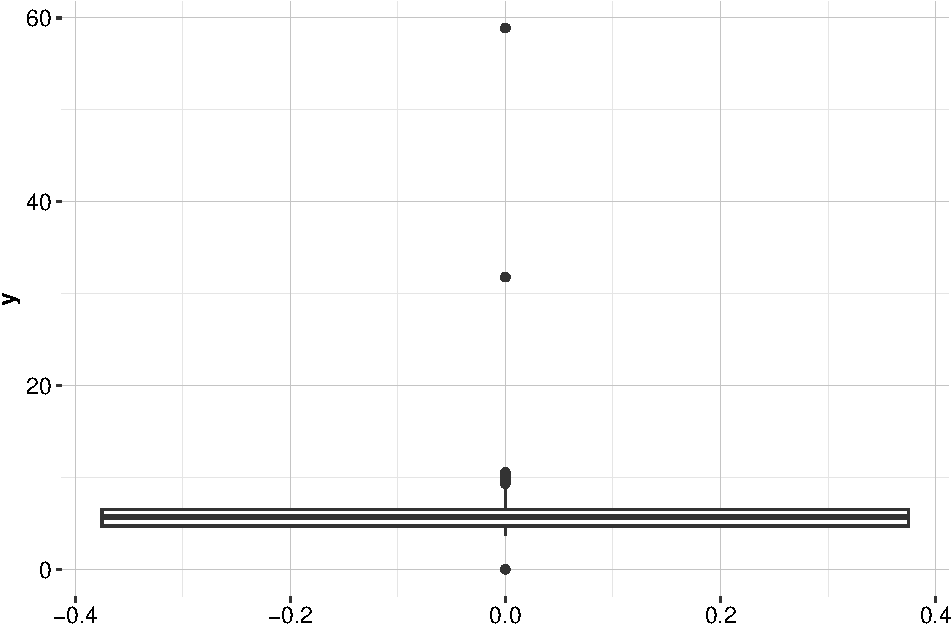
\includegraphics[width=0.7\linewidth]{data-preparation_files/figure-latex/unnamed-chunk-4-1} \end{center}

Here, boxplots highlight values beyond the whiskers, which may indicate potential outliers. Since diamonds cannot have a width of 0 mm, values like 32 mm or 59 mm likely result from data entry errors.

\subsubsection*{Histograms: Understanding Outlier Distribution}\label{histograms-understanding-outlier-distribution}
\addcontentsline{toc}{subsubsection}{Histograms: Understanding Outlier Distribution}

Histograms provide another visual approach to detecting outliers by displaying the frequency distribution of values. Below is a histogram of the \passthrough{\lstinline!y!} variable by using the \emph{ggplot()} and \emph{geom\_histogram()} functions:

\begin{lstlisting}[language=R]
ggplot(data = diamonds) +
    geom_histogram(aes(x = y), binwidth = 0.5, color = 'blue', fill = "lightblue")
\end{lstlisting}

\begin{center}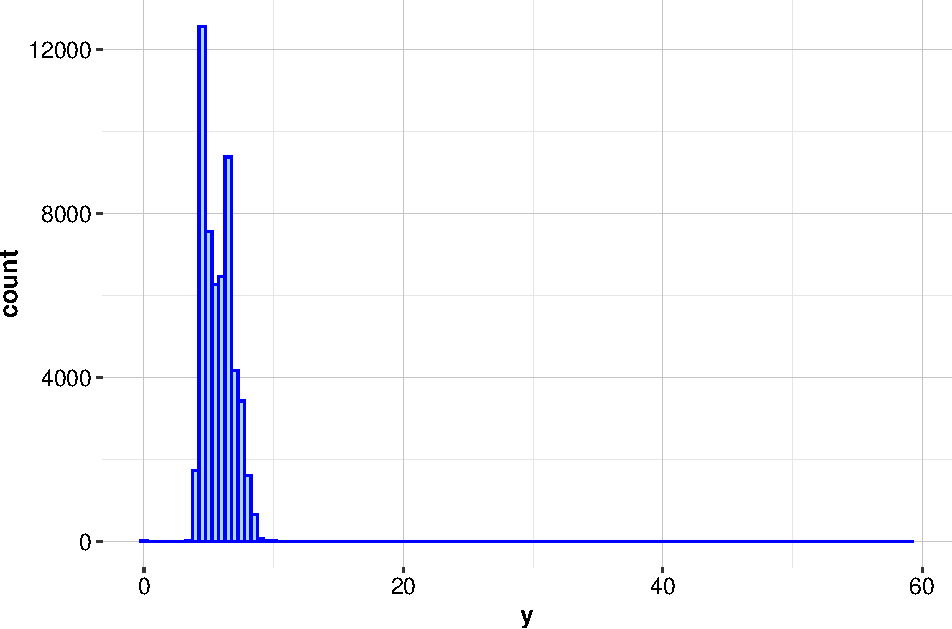
\includegraphics[width=0.7\linewidth]{data-preparation_files/figure-latex/unnamed-chunk-5-1} \end{center}

To enhance visibility, we can zoom in on smaller frequencies by using the \emph{coord\_cartesian()} function from the \textbf{ggplot2} package:

\begin{lstlisting}[language=R]
ggplot(data = diamonds) +
    geom_histogram(mapping = aes(x = y), binwidth = 0.5, color = 'blue', fill = "lightblue") + 
    coord_cartesian(ylim = c(0, 30))
\end{lstlisting}

\begin{center}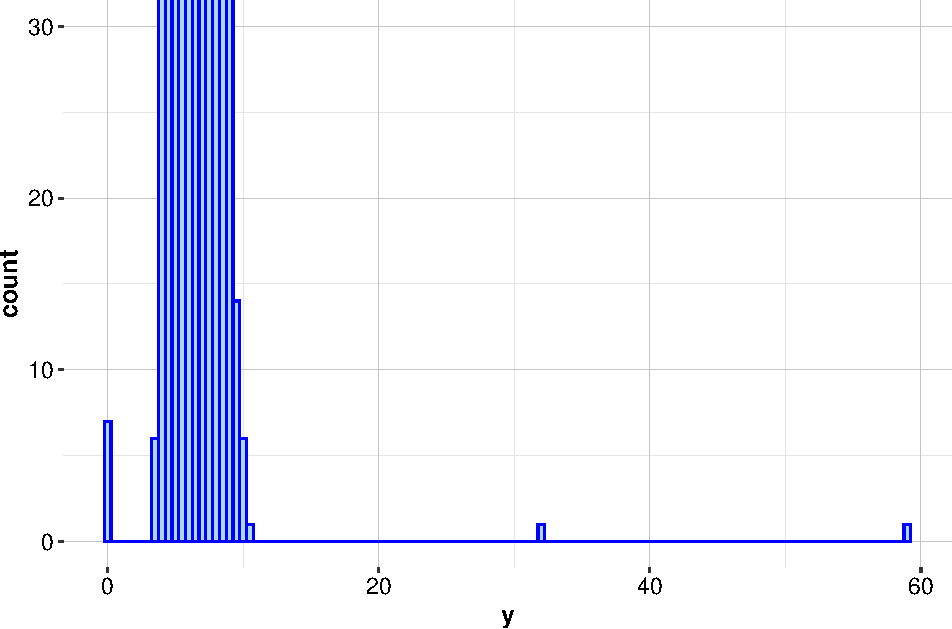
\includegraphics[width=0.7\linewidth]{data-preparation_files/figure-latex/unnamed-chunk-6-1} \end{center}

Other useful visualization techniques include:

\begin{itemize}
\tightlist
\item
  Violin plots -- Show both outliers and density distributions.
\item
  Density plots -- Provide smoother insights into rare values and multimodal distributions.
\end{itemize}

\subsection*{Handling Outliers: Best Practices}\label{handling-outliers-best-practices}
\addcontentsline{toc}{subsection}{Handling Outliers: Best Practices}

Once outliers are identified, there are several strategies for handling them:

\begin{enumerate}
\def\labelenumi{\arabic{enumi}.}
\tightlist
\item
  \emph{Removing outliers}: This is appropriate when an outlier is clearly an error (e.g., negative height, duplicate data entry).
\item
  \emph{Transforming values}: Techniques such as log transformation or square root scaling can reduce the influence of extreme values while preserving trends.
\item
  \emph{Winsorization}: Instead of removing outliers, replace them with the nearest percentile-based value (e.g., capping extreme values at the 95th percentile).
\item
  \emph{Using robust statistical methods}: Some algorithms, like median-based regression or random forests, are less sensitive to outliers.
\item
  \emph{Treating outliers as a separate category}: In fraud detection or rare event prediction, outliers may contain valuable insights and should not be removed.
\end{enumerate}

Choosing the right strategy depends on the context of the analysis and the potential impact of the outlier.

\subsection*{Expanded Code Example: Handling Outliers in R}\label{expanded-code-example-handling-outliers-in-r}
\addcontentsline{toc}{subsection}{Expanded Code Example: Handling Outliers in R}

After detecting outliers, we can choose to either replace them with \passthrough{\lstinline!NA!} values or remove them. For this, we could consider using the \passthrough{\lstinline!mutate()!} function from the \textbf{dplyr} package. Here's an example of treating outliers as missing values using \passthrough{\lstinline!mutate()!} and \passthrough{\lstinline!ifelse()!}:

\begin{lstlisting}[language=R]
diamonds_2 <- mutate(diamonds, y = ifelse(y == 0 | y > 30, NA, y))
\end{lstlisting}

Here's how to verify the update:

\begin{lstlisting}[language=R]
summary(diamonds_2$y)
      Min. 1st Qu.  Median    Mean 3rd Qu.    Max.    NA's 
     3.680   4.720   5.710   5.734   6.540  10.540       9
\end{lstlisting}

This method ensures that outliers do not distort the dataset while allowing for further imputation or analysis.

\section{Missing Values}\label{missing-values}

Missing values pose significant challenges in data analysis, as they can lead to biased results, reduce statistical power, and impact the performance of machine learning models. When handling missing data, we typically consider two approaches:

\begin{enumerate}
\def\labelenumi{\arabic{enumi}.}
\tightlist
\item
  Imputation: Replacing missing values with estimated values to retain data integrity.\\
\item
  Removal: Deleting records with missing values, though this may lead to data loss and potential bias.
\end{enumerate}

\subsection*{Imputation Techniques}\label{imputation-techniques}
\addcontentsline{toc}{subsection}{Imputation Techniques}

There are several strategies for imputing missing values, each with different use cases:

\begin{itemize}
\tightlist
\item
  Mean, median, or mode imputation: Replaces missing values with the mean, median, or mode of the corresponding column.\\
\item
  Random sampling: Fills missing values with random observations drawn from the existing data distribution.\\
\item
  Predictive imputation: Uses machine learning models such as regression or k-nearest neighbors to estimate missing values.\\
\item
  Multiple imputation: Generates several possible values for missing entries and averages the results to reduce uncertainty.\\
  \#\#\# Example: Random Sampling Imputation in R \{-\}
\end{itemize}

To impute missing values in \passthrough{\lstinline!y!} using random sampling, we use the \passthrough{\lstinline!impute()!} function from the \textbf{Hmisc} package:

\begin{lstlisting}[language=R]
diamonds_2$y <- impute(diamonds_2$y, "random")
\end{lstlisting}

The \passthrough{\lstinline!impute()!} function replaces missing values with randomly sampled values from the existing distribution of \passthrough{\lstinline!y!}, maintaining the overall statistical properties of the dataset.

\subsection*{Best Practices}\label{best-practices}
\addcontentsline{toc}{subsection}{Best Practices}

\begin{itemize}
\tightlist
\item
  Use mean or median imputation for numerical variables when the missing values are missing at random (MAR).\\
\item
  Use mode imputation for categorical variables.\\
\item
  Consider predictive models when the dataset is large and missing values are not completely random.\\
\item
  Always assess the proportion of missing data---if too many values are missing, removing the variable may be a better approach than imputation.
\end{itemize}

\section{Feature Scaling}\label{feature-scaling}

Feature scaling, also known as normalization or standardization, is a crucial step in data preprocessing. It adjusts the range and distribution of numerical features so they are on a similar scale. Many machine learning algorithms, especially those based on distance metrics such as k-nearest neighbors, benefit significantly from scaled input features, as this prevents variables with larger ranges from disproportionately influencing the model's outcome.

For instance, in the \emph{diamonds} dataset, the \passthrough{\lstinline!carat!} variable ranges from 0.2 to 5, while \passthrough{\lstinline!price!} ranges from 326 to 18823. Without scaling, variables like \passthrough{\lstinline!price!} with a wider range can dominate the model's predictions, potentially leading to suboptimal results. To address this, we apply feature scaling techniques to bring all numeric variables onto a comparable scale. In this section, we explore two common scaling methods:

\begin{enumerate}
\def\labelenumi{\arabic{enumi}.}
\tightlist
\item
  \emph{Min-Max Scaling}: Also known as min-max normalization or min-max transformation.
\item
  \emph{Z-score Scaling}: Also known as standardization or Z-score normalization.
\end{enumerate}

Feature scaling provides several benefits:

\begin{itemize}
\tightlist
\item
  \emph{Improved Model Performance}: Ensures that features contribute equally to the model, preventing features with larger numerical ranges from dominating learning algorithms.
\item
  \emph{Better Model Convergence}: Particularly useful for gradient-based optimization methods such as logistic regression and neural networks.
\item
  \emph{More Effective Distance-Based Learning}: Algorithms such as k-means clustering and support vector machines rely on distance calculations, making feature scaling essential.
\item
  \emph{Consistent Feature Interpretation}: By standardizing numerical values, models become easier to compare and interpret.
\end{itemize}

However, feature scaling also has some drawbacks:

\begin{itemize}
\tightlist
\item
  \emph{Potential Loss of Information}: In some cases, scaling can obscure meaningful differences between data points.
\item
  \emph{Impact on Outliers}: Min-max scaling, in particular, is sensitive to extreme values, which can distort the scaled representation.
\item
  \emph{Additional Computation}: Scaling adds preprocessing overhead, particularly when working with large datasets.
\item
  \emph{Reduced Interpretability}: The original units of measurement are lost, making it harder to relate scaled values to real-world meanings.
\end{itemize}

Selecting the right scaling method depends on the characteristics of the data and the requirements of the model. In the next sections, we will explore these methods in more detail and apply them to the \emph{diamonds} dataset.

\section{Min-Max Scaling}\label{min-max-scaling}

Min-Max Scaling transforms the values of a feature to a fixed range, typically \([0, 1]\). This transformation ensures that the minimum value of each feature becomes 0 and the maximum value becomes 1. It is especially useful for algorithms that rely on distance metrics, as it equalizes the contributions of all features, making comparisons more balanced.

The formula for Min-Max Scaling is:

\[
x_{\text{scaled}} = \frac{x - x_{\text{min}}}{x_{\text{max}} - x_{\text{min}}},
\]
where \(x\) is the original feature value, \(x_{\text{min}}\) and \(x_{\text{max}}\) are the minimum and maximum values of the feature, and \(x_{\text{scaled}}\) is the scaled value, ranging between 0 and 1.

Min-Max Scaling is particularly useful for models that require bounded input values, such as neural networks and algorithms relying on gradient-based optimization. However, this method is sensitive to outliers, as extreme values significantly affect the scaled distribution.

\begin{example}
\protect\hypertarget{exm:ex-min-max}{}\label{exm:ex-min-max}To demonstrate Min-Max Scaling, we'll apply it to the \passthrough{\lstinline!carat!} variable in the \emph{diamonds} dataset, where \passthrough{\lstinline!carat!} values range from approximately 0.2 to 5. Using the \passthrough{\lstinline!minmax()!} function from the \textbf{liver} package, we can scale \passthrough{\lstinline!carat!} values to fit within the range {[}0, 1{]}.

\begin{lstlisting}[language=R]
ggplot(data = diamonds) +
  geom_histogram(mapping = aes(x = carat), bins = 30,
                 color = 'blue', fill = "lightblue") +
  ggtitle("Histogram for `carat` without scaling") + 
  xlab("Values for variable `carat`")

ggplot(data = diamonds) +
  geom_histogram(mapping = aes(x = minmax(carat)), bins = 30,
                 color = 'blue', fill = "lightblue") +
  ggtitle("Histogram for `carat` with Min-Max Scaling") + 
  xlab("Values for variable `carat`")
\end{lstlisting}

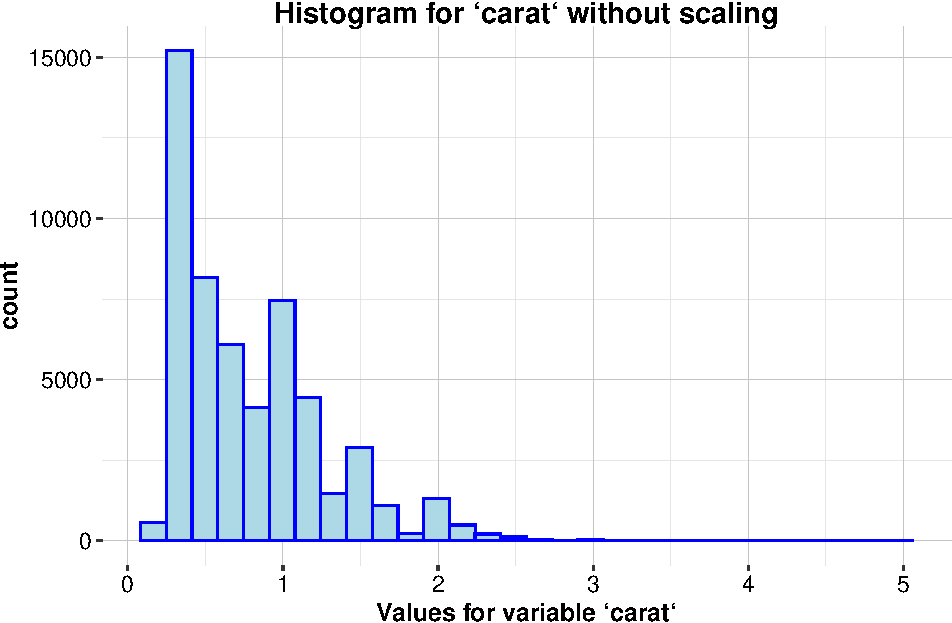
\includegraphics[width=0.5\linewidth]{data-preparation_files/figure-latex/unnamed-chunk-10-1} 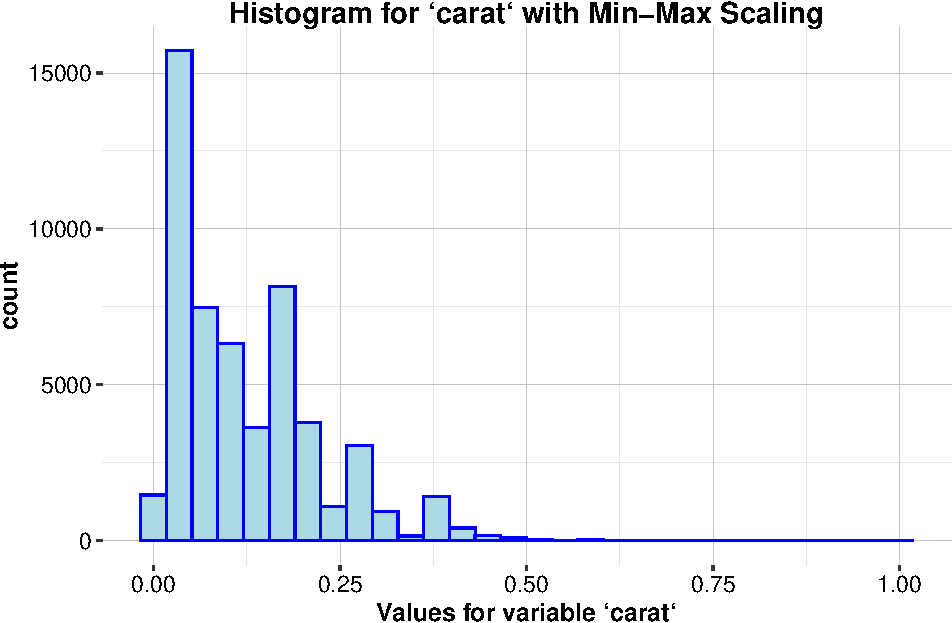
\includegraphics[width=0.5\linewidth]{data-preparation_files/figure-latex/unnamed-chunk-10-2}

The first histogram (left) shows the distribution of \passthrough{\lstinline!carat!} without scaling, while the second histogram (right) shows it after Min-Max Scaling. After scaling, the \passthrough{\lstinline!carat!} values are compressed to a range between 0 and 1, allowing it to be more comparable to other features that may have different original scales. This scaling method is particularly beneficial for distance-based algorithms, as it prevents features with wider ranges from having undue influence.
\end{example}

\section{Z-score Scaling}\label{z-score-scaling}

Z-score Scaling, also known as standardization, transforms feature values so they have a mean of 0 and a standard deviation of 1. This method is particularly useful for algorithms that assume normally distributed data, such as linear regression and logistic regression, because it centers the data around 0 and normalizes the spread of values.

The formula for Z-score Scaling is:

\[
x_{\text{scaled}} = \frac{x - \text{mean}(x)}{\text{sd}(x)}
\]

where \(x\) is the original feature value, \(\text{mean}(x)\) is the mean of the feature, \(\text{sd}(x)\) is the standard deviation of the feature, and \(x_{\text{scaled}}\) is the standardized value, now having a mean of 0 and a standard deviation of 1.

Z-score Scaling is particularly beneficial for models that assume normality or use gradient-based optimization, ensuring that all numerical features contribute equally. However, since it relies on mean and standard deviation, it is \textbf{sensitive to outliers}, which can distort the transformation.

\begin{example}
\protect\hypertarget{exm:ex-zscore}{}\label{exm:ex-zscore}Applying Z-score Scaling to the \passthrough{\lstinline!carat!} variable in the \emph{diamonds} dataset, where the mean and standard deviation of \passthrough{\lstinline!carat!} are approximately 0.8 and 0.47, respectively. We use the \passthrough{\lstinline!zscore()!} function from the \textbf{liver} package to standardize these values.

\begin{lstlisting}[language=R]
ggplot(data = diamonds) +
  geom_histogram(mapping = aes(x = carat), bins = 30,
                 color = 'blue', fill = "lightblue") +
  ggtitle("Histogram for `carat` without scaling") + 
  xlab("Values for variable `carat`")

ggplot(data = diamonds) +
  geom_histogram(mapping = aes(x = zscore(carat)), bins = 30,
                 color = 'blue', fill = "lightblue") +
  ggtitle("Histogram for `carat` with Z-score Scaling") + 
  xlab("Values for variable `carat`")
\end{lstlisting}

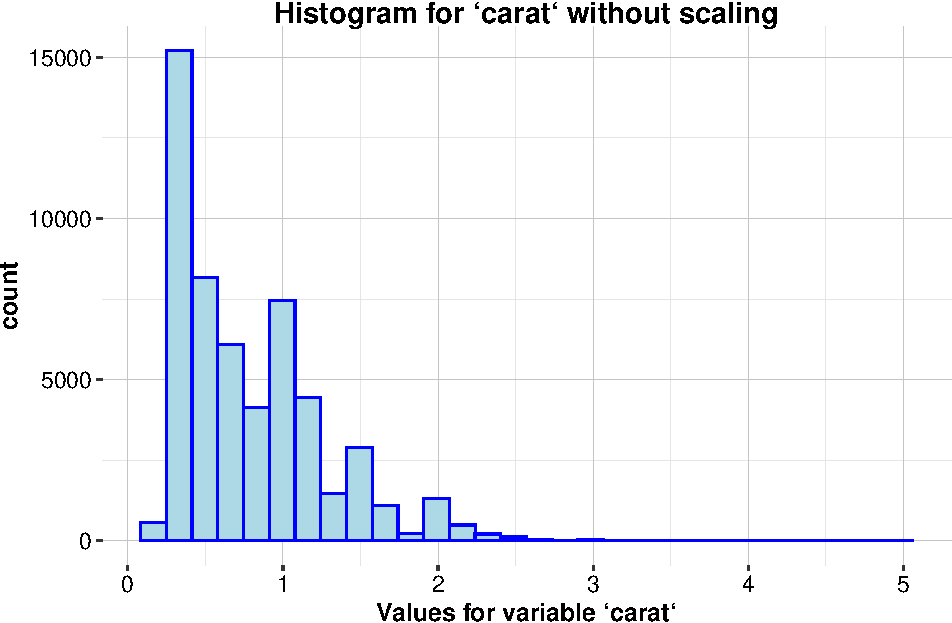
\includegraphics[width=0.5\linewidth]{data-preparation_files/figure-latex/unnamed-chunk-11-1} 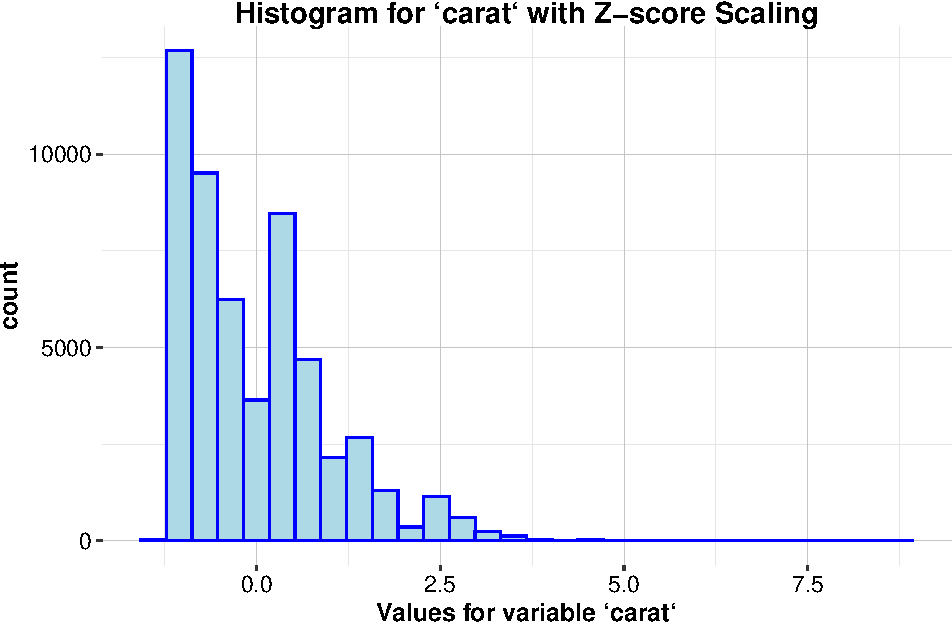
\includegraphics[width=0.5\linewidth]{data-preparation_files/figure-latex/unnamed-chunk-11-2}

The first histogram (left) displays the distribution of \passthrough{\lstinline!carat!} without scaling, while the second histogram (right) shows the distribution after Z-score Scaling. This transformation makes feature values comparable across different scales and ensures that each feature contributes equally to distance-based computations and model training.
\end{example}

\begin{quote}
Note: A common misconception is that after Z-score Scaling, the data follows a standard normal distribution. While Z-score Scaling centers the data to a mean of 0 and scales it to a standard deviation of 1, it does not alter the shape of the distribution. If the original distribution is skewed, it will remain skewed after scaling, as seen in the histograms above.
\end{quote}

The choice between Min-Max Scaling and Z-score Scaling depends on the requirements of the model and the characteristics of the data. Min-Max Scaling is preferable for algorithms that require a fixed input range, while Z-score Scaling is better suited for models that assume normally distributed features. By selecting the appropriate scaling method, we ensure balanced feature contributions and improved model performance.

\section{How to Reexpress Categorical Field Values}\label{how-to-reexpress-categorical-field-values}

In data science, categorical features often need to be transformed into a numeric format before they can be used in machine learning models. Algorithms like decision trees, neural networks, and linear regression require numeric inputs to process the data effectively. Converting categorical variables into numerical representations ensures that all features contribute appropriately to the model, rather than being ignored or treated incorrectly.

This process of reexpressing categorical values is a crucial part of data preparation, as it enables us to leverage the full range of features in our dataset. In this section, we explore several methods to convert categorical fields into numeric representations, with a focus on techniques like one-hot encoding and ordinal encoding. We demonstrate these techniques using the \emph{diamonds} dataset, which includes several categorical features such as \passthrough{\lstinline!cut!}, \passthrough{\lstinline!color!}, and \passthrough{\lstinline!clarity!}.

\subsection{Why Reexpress Categorical Fields?}\label{why-reexpress-categorical-fields}

Categorical fields, also known as nominal or ordinal variables, often represent qualitative aspects of data, such as product types, user locations, or levels of satisfaction. In the \emph{diamonds} dataset, for example:

\begin{itemize}
\tightlist
\item
  \passthrough{\lstinline!cut!} indicates the quality of the diamond's cut (e.g., ``Fair,'' ``Good,'' ``Very Good,'' ``Premium,'' ``Ideal'').
\item
  \passthrough{\lstinline!color!} represents the diamond's color grade (e.g., ``D,'' ``E,'' ``F,'' with ``D'' being the most colorless and thus most valuable).
\item
  \passthrough{\lstinline!clarity!} describes the diamond's clarity, reflecting the absence of internal or external flaws.
\end{itemize}

These fields are essential for understanding and predicting diamond pricing, but in their raw form as text labels, they are not suitable for most machine learning algorithms. Transforming them into numeric form allows us to include these valuable insights in our analysis.

\subsection{Techniques for Reexpressing Categorical Variables}\label{techniques-for-reexpressing-categorical-variables}

There are several approaches to converting categorical variables into numeric representations. The method we choose depends on the type of categorical variable and the nature of the data.

\subsubsection*{Ordinal Encoding}\label{ordinal-encoding}
\addcontentsline{toc}{subsubsection}{Ordinal Encoding}

Ordinal encoding is suitable when the categorical variable has a meaningful order. For example, the \passthrough{\lstinline!cut!} feature in the \emph{diamonds} dataset is ordinal, as there is a natural hierarchy from ``Fair'' to ``Ideal.'' In ordinal encoding, each category is assigned a unique integer based on its rank or level of importance.

In this example, we might assign values as follows:

\begin{itemize}
\tightlist
\item
  ``Fair'' → 1
\item
  ``Good'' → 2
\item
  ``Very Good'' → 3
\item
  ``Premium'' → 4
\item
  ``Ideal'' → 5
\end{itemize}

This approach preserves the order of the categories, which can be useful in models that interpret numeric values in a relative way, such as linear regression. However, it is important to apply ordinal encoding only when the order is meaningful. For non-ordinal variables, other methods like one-hot encoding are more appropriate.

\subsubsection*{One-Hot Encoding}\label{one-hot-encoding}
\addcontentsline{toc}{subsubsection}{One-Hot Encoding}

One-hot encoding is the preferred technique for nominal variables---categorical fields without an intrinsic order. In this approach, each unique category in a field is transformed into a new binary (0 or 1) feature. This method is particularly useful for variables like \passthrough{\lstinline!color!} and \passthrough{\lstinline!clarity!} in the \emph{diamonds} dataset, where the categories do not follow a clear sequence.

For example, if we one-hot encode the \passthrough{\lstinline!color!} feature, we create a set of binary columns, one for each color grade:

\begin{itemize}
\tightlist
\item
  \passthrough{\lstinline!color\_D!}: 1 if the diamond color is ``D,'' 0 otherwise.
\item
  \passthrough{\lstinline!color\_E!}: 1 if the diamond color is ``E,'' 0 otherwise.
\item
  \passthrough{\lstinline!color\_F!}: 1 if the diamond color is ``F,'' 0 otherwise.
\end{itemize}

One-hot encoding avoids introducing false ordinal relationships, ensuring that the model treats each category as an independent entity. However, one downside is that it can significantly increase the dimensionality of the dataset if the categorical field has many unique values.

\begin{quote}
Note: Many machine learning libraries automatically drop one of the binary columns to avoid multicollinearity (perfect correlation among features). For instance, if we have seven color categories, only six binary columns are created, and the missing category is implied when all columns are zero. This approach, known as dummy encoding, helps avoid redundancy and keeps the model simpler.
\end{quote}

\subsubsection*{Frequency Encoding}\label{frequency-encoding}
\addcontentsline{toc}{subsubsection}{Frequency Encoding}

Another useful approach, especially for high-cardinality categorical variables (those with many unique values), is frequency encoding. This technique replaces each category with its frequency in the dataset, allowing the model to capture information about how common each category is. Frequency encoding can be particularly helpful for fields like \passthrough{\lstinline!clarity!} if you want to give the model an indication of how prevalent each level is.

For example:

\begin{itemize}
\tightlist
\item
  If ``VS2'' appears 10,000 times in the dataset, it would be encoded as 10,000.
\item
  If ``IF'' appears only 500 times, it would be encoded as 500.
\end{itemize}

Frequency encoding is less commonly used in basic machine learning workflows but can be valuable when dealing with very large datasets, or when one-hot encoding would introduce too many columns. However, be cautious with this approach, as it may inadvertently add an implicit weight to more common categories.

\subsection{Choosing the Right Encoding Technique}\label{choosing-the-right-encoding-technique}

Selecting the appropriate encoding technique depends on the nature of your categorical variable and the requirements of your analysis:

\begin{itemize}
\tightlist
\item
  Ordinal variables (like \passthrough{\lstinline!cut!}): Use ordinal encoding to preserve the natural order.
\item
  Nominal variables with few unique values (like \passthrough{\lstinline!color!} and \passthrough{\lstinline!clarity!}): Use one-hot encoding to represent each category as a binary column.
\item
  High-cardinality categorical variables: Consider frequency encoding if one-hot encoding would introduce too many features.
\end{itemize}

\begin{example}
\protect\hypertarget{exm:ex-encoding}{}\label{exm:ex-encoding}

Applying these techniques to the \emph{diamonds} dataset:

\begin{lstlisting}[language=R]
# Example: Ordinal encoding for `cut`
diamonds <- diamonds %>%
  mutate(cut_encoded = as.integer(factor(cut, levels = c("Fair", "Good", "Very Good", "Premium", "Ideal"))))

# Example: One-hot encoding for `color`
diamonds <- diamonds %>%
  mutate(
    color_D = ifelse(color == "D", 1, 0),
    color_E = ifelse(color == "E", 1, 0),
    color_F = ifelse(color == "F", 1, 0),
    color_G = ifelse(color == "G", 1, 0),
    color_H = ifelse(color == "H", 1, 0),
    color_I = ifelse(color == "I", 1, 0),
    color_J = ifelse(color == "J", 1, 0)
  )
\end{lstlisting}

In this example:

\begin{itemize}
\tightlist
\item
  Ordinal Encoding: We have encoded the \passthrough{\lstinline!cut!} variable based on its quality hierarchy.
\item
  One-Hot Encoding: We have applied one-hot encoding to \passthrough{\lstinline!color!}, creating binary columns for each color grade.
\end{itemize}

\end{example}

By encoding the categorical fields in this way, we transform the dataset into a format compatible with most machine learning algorithms while preserving the essential information about each categorical feature.

With our dataset now cleaned, scaled, and encoded, we are ready to move into the next stage of data analysis. In the upcoming chapter, we will explore Exploratory Data Analysis (EDA), where we will use visualizations and summary statistics to gain insights into the structure and relationships within the data. By combining the prepared data with EDA techniques, we can better understand which features may hold predictive value for our model and set the stage for successful machine learning outcomes.

\section{Case Study: Who Can Earn More Than \$50K Per Year?}\label{Data-pre-adult}

In this case study, we will explore the \emph{Adult} dataset, sourced from the \href{https://www.census.gov}{US Census Bureau}. This dataset contains demographic information about individuals, including age, education, occupation, and income. The dataset is available in the \textbf{liver} package. For more details, refer to the \href{https://www.rdocumentation.org/packages/liver/versions/1.3/topics/adult}{documentation}.

The goal of this study is to predict whether an individual earns more than \$50,000 per year based on their attributes. In Section \ref{tree-case-study} of Chapter \ref{chapter-tree}, we will apply decision tree and random forest algorithms to build a predictive model. Before applying these techniques, we need to preprocess the dataset by handling missing values, encoding categorical variables, and scaling numerical features. Let's begin by loading the dataset and examining its structure.

\subsection*{Overview of the Dataset}\label{overview-of-the-dataset}
\addcontentsline{toc}{subsection}{Overview of the Dataset}

To use the \emph{Adult} dataset, first ensure that the \textbf{liver} package is installed. If not, install it using:

\begin{lstlisting}[language=R]
install.packages("liver")
\end{lstlisting}

Next, load the package and dataset:

\begin{lstlisting}[language=R]
library(liver)  # Load liver package
data(adult)     # Load Adult dataset
\end{lstlisting}

To inspect the dataset structure, use:

\begin{lstlisting}[language=R]
str(adult)
   'data.frame':    48598 obs. of  15 variables:
    $ age           : int  25 38 28 44 18 34 29 63 24 55 ...
    $ workclass     : Factor w/ 6 levels "?","Gov","Never-worked",..: 4 4 2 4 1 4 1 5 4 4 ...
    $ demogweight   : int  226802 89814 336951 160323 103497 198693 227026 104626 369667 104996 ...
    $ education     : Factor w/ 16 levels "10th","11th",..: 2 12 8 16 16 1 12 15 16 6 ...
    $ education.num : int  7 9 12 10 10 6 9 15 10 4 ...
    $ marital.status: Factor w/ 5 levels "Divorced","Married",..: 3 2 2 2 3 3 3 2 3 2 ...
    $ occupation    : Factor w/ 15 levels "?","Adm-clerical",..: 8 6 12 8 1 9 1 11 9 4 ...
    $ relationship  : Factor w/ 6 levels "Husband","Not-in-family",..: 4 1 1 1 4 2 5 1 5 1 ...
    $ race          : Factor w/ 5 levels "Amer-Indian-Eskimo",..: 3 5 5 3 5 5 3 5 5 5 ...
    $ gender        : Factor w/ 2 levels "Female","Male": 2 2 2 2 1 2 2 2 1 2 ...
    $ capital.gain  : int  0 0 0 7688 0 0 0 3103 0 0 ...
    $ capital.loss  : int  0 0 0 0 0 0 0 0 0 0 ...
    $ hours.per.week: int  40 50 40 40 30 30 40 32 40 10 ...
    $ native.country: Factor w/ 42 levels "?","Cambodia",..: 40 40 40 40 40 40 40 40 40 40 ...
    $ income        : Factor w/ 2 levels "<=50K",">50K": 1 1 2 2 1 1 1 2 1 1 ...
\end{lstlisting}

The dataset contains 48598 records and 15 variables. Of these, 14 are predictors, while the target variable, \passthrough{\lstinline!income!}, is a categorical variable with two levels: \passthrough{\lstinline!<=50K!} and \passthrough{\lstinline!>50K!}. The features include both numerical and categorical variables:

\begin{itemize}
\tightlist
\item
  \passthrough{\lstinline!age!}: Age in years (numerical).\\
\item
  \passthrough{\lstinline!workclass!}: Employment type (categorical, 6 levels).\\
\item
  \passthrough{\lstinline!demogweight!}: Census weighting factor (numerical).\\
\item
  \passthrough{\lstinline!education!}: Highest level of education (categorical, 16 levels).\\
\item
  \passthrough{\lstinline!education.num!}: Number of years of education (numerical).\\
\item
  \passthrough{\lstinline!marital.status!}: Marital status (categorical, 5 levels).\\
\item
  \passthrough{\lstinline!occupation!}: Job category (categorical, 15 levels).\\
\item
  \passthrough{\lstinline!relationship!}: Family relationship status (categorical, 6 levels).\\
\item
  \passthrough{\lstinline!race!}: Racial background (categorical, 5 levels).\\
\item
  \passthrough{\lstinline!gender!}: Gender identity (categorical, Male/Female).\\
\item
  \passthrough{\lstinline!capital.gain!}: Capital gains (numerical).\\
\item
  \passthrough{\lstinline!capital.loss!}: Capital losses (numerical).\\
\item
  \passthrough{\lstinline!hours.per.week!}: Hours worked per week (numerical).\\
\item
  \passthrough{\lstinline!native.country!}: Country of origin (categorical, 42 levels).\\
\item
  \passthrough{\lstinline!income!}: Target variable indicating annual income (\passthrough{\lstinline!<=50K!} or \passthrough{\lstinline!>50K!}).
\end{itemize}

For clarity, we categorize the dataset's variables:

\begin{itemize}
\tightlist
\item
  \textbf{Nominal variables}: \passthrough{\lstinline!workclass!}, \passthrough{\lstinline!marital.status!}, \passthrough{\lstinline!occupation!}, \passthrough{\lstinline!relationship!}, \passthrough{\lstinline!race!}, \passthrough{\lstinline!native.country!}, and \passthrough{\lstinline!gender!}.\\
\item
  \textbf{Ordinal variable}: \passthrough{\lstinline!education!}.\\
\item
  \textbf{Numerical variables}: \passthrough{\lstinline!age!}, \passthrough{\lstinline!demogweight!}, \passthrough{\lstinline!education.num!}, \passthrough{\lstinline!capital.gain!}, \passthrough{\lstinline!capital.loss!}, and \passthrough{\lstinline!hours.per.week!}.
\end{itemize}

To better understand the dataset, we generate summary statistics:

\begin{lstlisting}[language=R]
summary(adult)
         age              workclass      demogweight             education    
    Min.   :17.0   ?           : 2794   Min.   :  12285   HS-grad     :15750  
    1st Qu.:28.0   Gov         : 6536   1st Qu.: 117550   Some-college:10860  
    Median :37.0   Never-worked:   10   Median : 178215   Bachelors   : 7962  
    Mean   :38.6   Private     :33780   Mean   : 189685   Masters     : 2627  
    3rd Qu.:48.0   Self-emp    : 5457   3rd Qu.: 237713   Assoc-voc   : 2058  
    Max.   :90.0   Without-pay :   21   Max.   :1490400   11th        : 1812  
                                                          (Other)     : 7529  
    education.num         marital.status            occupation   
    Min.   : 1.00   Divorced     : 6613   Craft-repair   : 6096  
    1st Qu.: 9.00   Married      :22847   Prof-specialty : 6071  
    Median :10.00   Never-married:16096   Exec-managerial: 6019  
    Mean   :10.06   Separated    : 1526   Adm-clerical   : 5603  
    3rd Qu.:12.00   Widowed      : 1516   Sales          : 5470  
    Max.   :16.00                         Other-service  : 4920  
                                          (Other)        :14419  
            relationship                   race          gender     
    Husband       :19537   Amer-Indian-Eskimo:  470   Female:16156  
    Not-in-family :12546   Asian-Pac-Islander: 1504   Male  :32442  
    Other-relative: 1506   Black             : 4675                 
    Own-child     : 7577   Other             :  403                 
    Unmarried     : 5118   White             :41546                 
    Wife          : 2314                                            
                                                                    
     capital.gain      capital.loss     hours.per.week        native.country 
    Min.   :    0.0   Min.   :   0.00   Min.   : 1.00   United-States:43613  
    1st Qu.:    0.0   1st Qu.:   0.00   1st Qu.:40.00   Mexico       :  949  
    Median :    0.0   Median :   0.00   Median :40.00   ?            :  847  
    Mean   :  582.4   Mean   :  87.94   Mean   :40.37   Philippines  :  292  
    3rd Qu.:    0.0   3rd Qu.:   0.00   3rd Qu.:45.00   Germany      :  206  
    Max.   :41310.0   Max.   :4356.00   Max.   :99.00   Puerto-Rico  :  184  
                                                        (Other)      : 2507  
      income     
    <=50K:37155  
    >50K :11443  
                 
                 
                 
                 
   
\end{lstlisting}

This summary provides insights into the distribution of numerical variables, missing values, and categorical variable levels, guiding us in preparing the data for further analysis.

\subsection{Missing Values}\label{missing-values-1}

The \passthrough{\lstinline!summary()!} function reveals that the variables \passthrough{\lstinline!workclass!} and \passthrough{\lstinline!native.country!} contain missing values, represented by the \passthrough{\lstinline!"?"!} category. Specifically, 2794 records in \passthrough{\lstinline!workclass!} and 847 records in \passthrough{\lstinline!native.country!} have missing values. Since \passthrough{\lstinline!"?"!} is used as a placeholder for missing data, we first convert these entries to \passthrough{\lstinline!NA!}:

\begin{lstlisting}[language=R]
adult[adult == "?"] = NA
\end{lstlisting}

After replacing \passthrough{\lstinline!"?"!} with \passthrough{\lstinline!NA!}, we remove unused factor levels to clean up the dataset:

\begin{lstlisting}[language=R]
adult = droplevels(adult)
\end{lstlisting}

To visualize the distribution of missing values, we use the \passthrough{\lstinline!gg\_miss\_var()!} function from the \textbf{naniar} package:

\begin{lstlisting}[language=R]
library(naniar)  # Load package for visualizing missing values

gg_miss_var(adult, show_pct = TRUE)
\end{lstlisting}

\begin{center}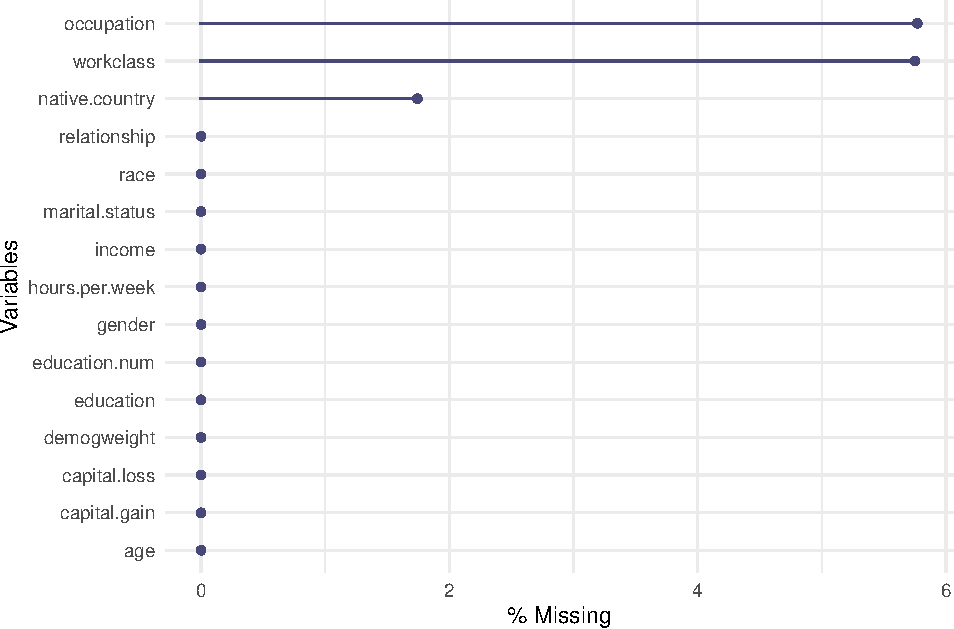
\includegraphics[width=0.7\linewidth]{data-preparation_files/figure-latex/unnamed-chunk-18-1} \end{center}

The plot indicates that \passthrough{\lstinline!workclass!}, \passthrough{\lstinline!occupation!}, and \passthrough{\lstinline!native.country!} contain missing values. The percentage of missing values in these variables is relatively low, with \passthrough{\lstinline!workclass!} and \passthrough{\lstinline!occupation!} having less than 0.06 percent missing data, while \passthrough{\lstinline!native.country!} has about 0.02 percent.

\subsubsection*{Imputing Missing Values}\label{imputing-missing-values}
\addcontentsline{toc}{subsubsection}{Imputing Missing Values}

Instead of removing records with missing values, which can lead to information loss, we apply \emph{random imputation}, where missing values are filled with randomly selected values from the existing distribution of each variable. This maintains the natural proportions of each category.

We use the \passthrough{\lstinline!impute()!} function from the \textbf{Hmisc} package for this purpose:

\begin{lstlisting}[language=R]
library(Hmisc)  # Load package for imputation

# Impute missing values using random sampling from existing categories
adult$workclass      = impute(adult$workclass,      'random')
adult$native.country = impute(adult$native.country, 'random')
adult$occupation     = impute(adult$occupation,     'random')
\end{lstlisting}

To confirm that missing values have been successfully imputed, we generate another missing values plot:

\begin{lstlisting}[language=R]
gg_miss_var(adult, show_pct = TRUE)
\end{lstlisting}

\begin{center}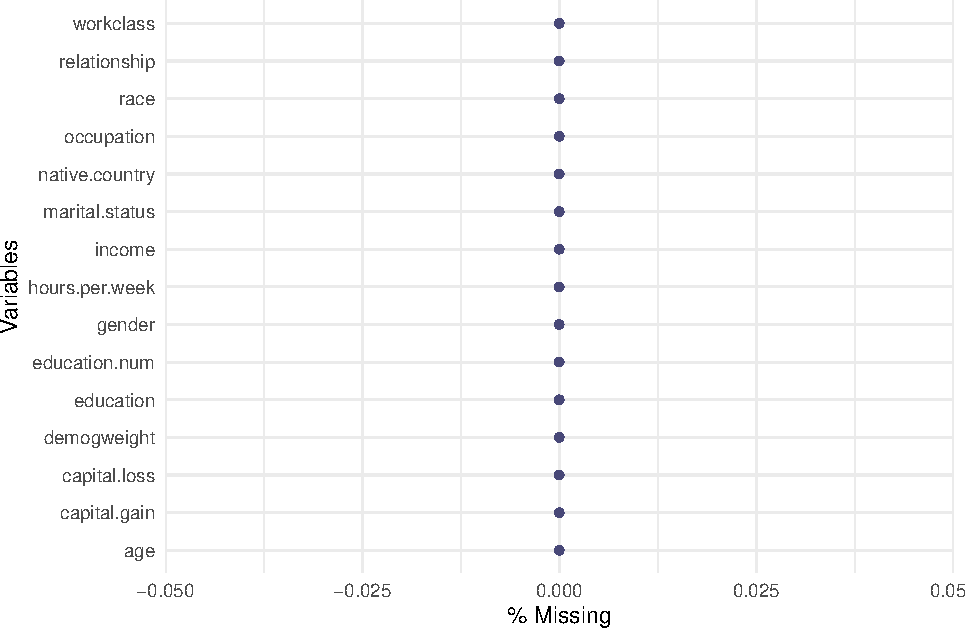
\includegraphics[width=0.7\linewidth]{data-preparation_files/figure-latex/unnamed-chunk-20-1} \end{center}

The updated plot should show no missing values, indicating successful imputation.

\subsubsection*{Alternative Approaches}\label{alternative-approaches}
\addcontentsline{toc}{subsubsection}{Alternative Approaches}

The \passthrough{\lstinline!impute()!} function allows for different statistical methods such as mean, median, or mode imputation. Its default behavior is \emph{median} imputation. For more advanced techniques, the \passthrough{\lstinline!aregImpute()!} function from the \textbf{Hmisc} package offers predictive imputation using additive regression, bootstrapping, and predictive mean matching.

Although removing records with missing values using \passthrough{\lstinline!na.omit()!} is an option, it is generally discouraged unless missing values are excessive or biased in a way that could distort analysis.

By properly handling missing values, we ensure data completeness and maintain the integrity of the dataset for subsequent preprocessing steps, such as recoding categorical variables and grouping country-level data into broader regions.

\subsection{Encoding Categorical Variables}\label{encoding-categorical-variables}

Categorical variables often contain a large number of unique values, making them challenging to use in predictive models. In the \emph{Adult} dataset, \passthrough{\lstinline!native.country!} and \passthrough{\lstinline!workclass!} have multiple categories, which can introduce complexity and redundancy. To simplify these variables, we group similar categories together while preserving their interpretability.

\subsubsection*{\texorpdfstring{Grouping \texttt{native.country} by Continent}{Grouping native.country by Continent}}\label{grouping-native.country-by-continent}
\addcontentsline{toc}{subsubsection}{Grouping \texttt{native.country} by Continent}

The \passthrough{\lstinline!native.country!} variable contains 41 distinct countries. To make it more manageable, we categorize countries into broader geographical regions:

\begin{itemize}
\tightlist
\item
  \textbf{Europe}: England, France, Germany, Greece, Netherlands, Hungary, Ireland, Italy, Poland, Portugal, Scotland, Yugoslavia\\
\item
  \textbf{Asia}: China, Hong Kong, India, Iran, Cambodia, Japan, Laos, Philippines, Vietnam, Taiwan, Thailand\\
\item
  \textbf{North America}: Canada, United States, Puerto Rico\\
\item
  \textbf{South America}: Colombia, Cuba, Dominican Republic, Ecuador, El Salvador, Guatemala, Haiti, Honduras, Mexico, Nicaragua, Outlying US territories, Peru, Jamaica, Trinidad \& Tobago\\
\item
  \textbf{Other}: This includes the ambiguous ``South'' category, as its meaning is unclear in the dataset documentation.\\
  We use the \passthrough{\lstinline!fct\_collapse()!} function from the \textbf{forcats} package to reassign categories:
\end{itemize}

\begin{lstlisting}[language=R]
library(forcats)  # Load package for categorical variable transformation

# To create a new factor variable with fewer levels for `native.country`
Europe = c("England", "France", "Germany", "Greece", "Holand-Netherlands", "Hungary", "Ireland", "Italy", "Poland", "Portugal", "Scotland", "Yugoslavia")

Asia = c("China", "Hong", "India", "Iran", "Cambodia", "Japan", "Laos", "Philippines", "Vietnam", "Taiwan", "Thailand")

N.America = c("Canada", "United-States", "Puerto-Rico")

S.America = c("Columbia", "Cuba", "Dominican-Republic", "Ecuador", "El-Salvador", "Guatemala", "Haiti", "Honduras", "Mexico", "Nicaragua", "Outlying-US(Guam-USVI-etc)", "Peru", "Jamaica", "Trinadad&Tobago")

# Reclassify native.country into broader regions
adult$native.country = fct_collapse(adult$native.country, 
                                    "Europe"    = Europe,
                                    "Asia"      = Asia,
                                    "N.America" = N.America,
                                    "S.America" = S.America,
                                    "Other"     = c("South") )
\end{lstlisting}

To confirm the changes, we display the frequency distribution of \passthrough{\lstinline!native.country!}:

\begin{lstlisting}[language=R]
table(adult$native.country)
   
        Asia N.America S.America    Europe     Other 
         993     44747      1946       797       115
\end{lstlisting}

By grouping the original 42 countries into 5 broader regions, we simplify the variable while maintaining its relevance for analysis.

\subsubsection*{\texorpdfstring{Simplifying \texttt{workclass}}{Simplifying workclass}}\label{simplifying-workclass}
\addcontentsline{toc}{subsubsection}{Simplifying \texttt{workclass}}

The \passthrough{\lstinline!workclass!} variable originally contains several employment categories. Since ``Never-worked'' and ``Without-pay'' represent similar employment statuses, we merge them into a single category labeled ``Unemployed'':

\begin{lstlisting}[language=R]
adult$workclass = fct_collapse(adult$workclass, "Unemployed" = c("Never-worked", "Without-pay"))
\end{lstlisting}

To verify the updated categories, we check the frequency distribution:

\begin{lstlisting}[language=R]
table(adult$workclass)
   
          Gov Unemployed    Private   Self-emp 
         6919         32      35851       5796
\end{lstlisting}

By reducing the number of unique categories in \passthrough{\lstinline!workclass!} and \passthrough{\lstinline!native.country!}, we improve model interpretability and reduce the risk of overfitting when applying machine learning algorithms.

\subsection{Outliers}\label{outliers}

Detecting and handling outliers is an essential step in data preprocessing, as extreme values can significantly impact statistical analysis and model performance. Here, we examine potential outliers in the \passthrough{\lstinline!capital.loss!} variable to determine whether adjustments are necessary.

\subsubsection*{Summary Statistics}\label{summary-statistics}
\addcontentsline{toc}{subsubsection}{Summary Statistics}

To gain an initial understanding of \passthrough{\lstinline!capital.loss!}, we compute its summary statistics:

\begin{lstlisting}[language=R]
summary(adult$capital.loss)
      Min. 1st Qu.  Median    Mean 3rd Qu.    Max. 
      0.00    0.00    0.00   87.94    0.00 4356.00
\end{lstlisting}

The summary output reveals the following insights:

\begin{itemize}
\tightlist
\item
  The minimum value is 0, while the maximum is 4356.\\
\item
  The \emph{median} is 0, which is significantly lower than the \emph{mean}, indicating a highly skewed distribution.\\
\item
  More than 75\% of the observations have a capital loss of 0, confirming a strong right-skew.\\
\item
  The mean capital loss is 87.94, which is influenced by a small number of extreme values.
\end{itemize}

\subsubsection*{Visualizing Outliers}\label{visualizing-outliers}
\addcontentsline{toc}{subsubsection}{Visualizing Outliers}

To further investigate the distribution of \passthrough{\lstinline!capital.loss!}, we use a boxplot and histogram:

\begin{lstlisting}[language=R]
ggplot(data = adult, aes(y = capital.loss)) +
     geom_boxplot()
\end{lstlisting}

\begin{center}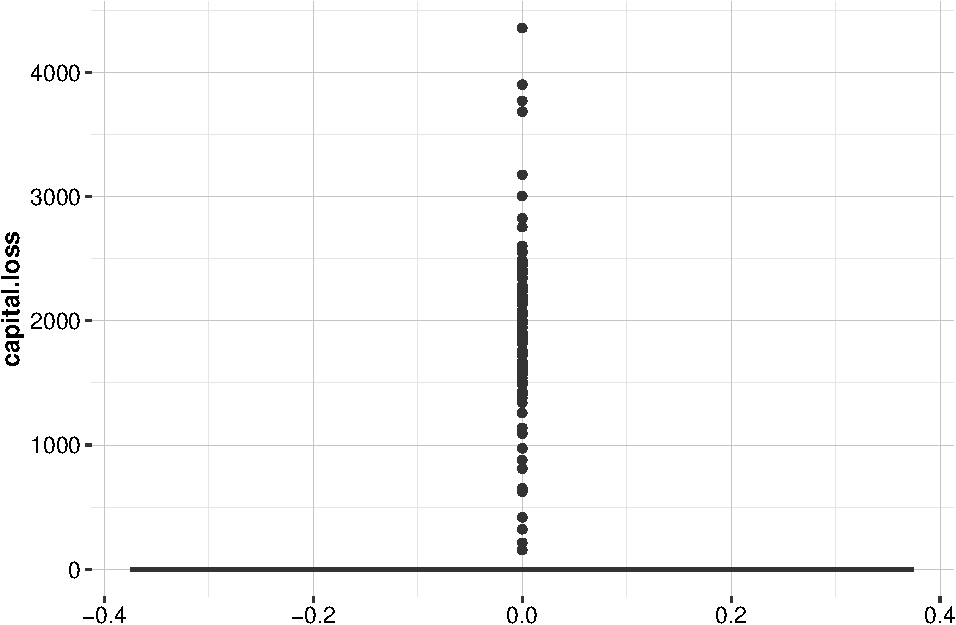
\includegraphics[width=0.7\linewidth]{data-preparation_files/figure-latex/unnamed-chunk-26-1} \end{center}

\begin{lstlisting}[language=R]
ggplot(data = adult, aes(x = capital.loss)) +
     geom_histogram(bins = 30, color = "blue", fill = "lightblue")
\end{lstlisting}

\begin{center}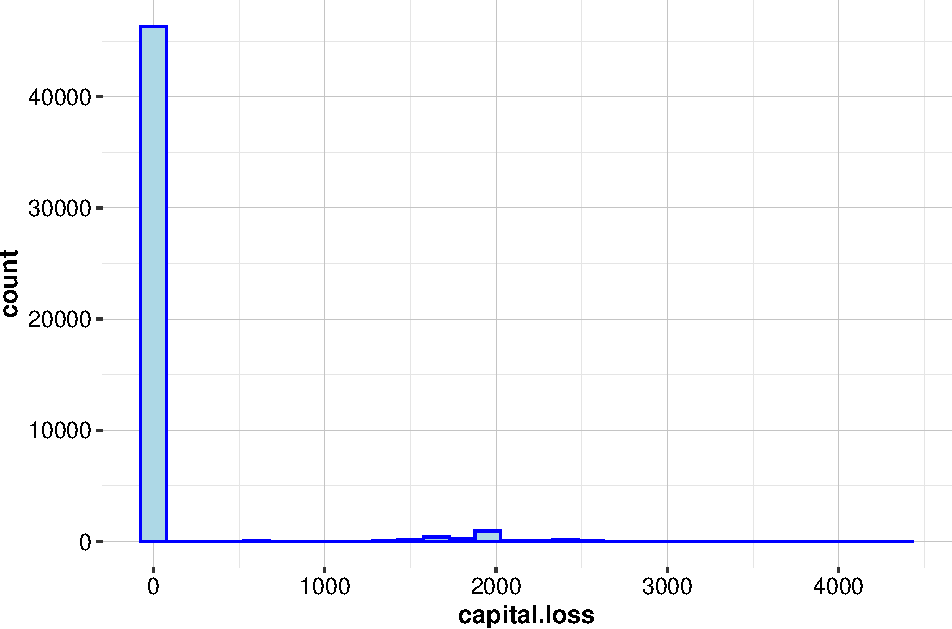
\includegraphics[width=0.7\linewidth]{data-preparation_files/figure-latex/unnamed-chunk-27-1} \end{center}

From these plots, we observe:

\begin{itemize}
\tightlist
\item
  The boxplot shows a strong \emph{positive skew}, with many extreme values above the upper whisker.\\
\item
  The histogram indicates that most observations have \emph{zero capital loss}, with a few cases around 2,000 and 4,000.
\end{itemize}

Since a large proportion of observations report no capital loss, we further examine the nonzero cases.

\subsubsection*{Zooming into the Nonzero Distribution}\label{zooming-into-the-nonzero-distribution}
\addcontentsline{toc}{subsubsection}{Zooming into the Nonzero Distribution}

To better visualize the spread of nonzero values, we focus on observations with \passthrough{\lstinline!capital.loss > 0!}:

\begin{lstlisting}[language=R]
ggplot(data = adult, mapping = aes(x = capital.loss)) +
    geom_histogram(bins = 30, color = "blue", fill = "lightblue") +
    coord_cartesian(xlim = c(500, 4000), ylim = c(0, 1000))
\end{lstlisting}

\begin{center}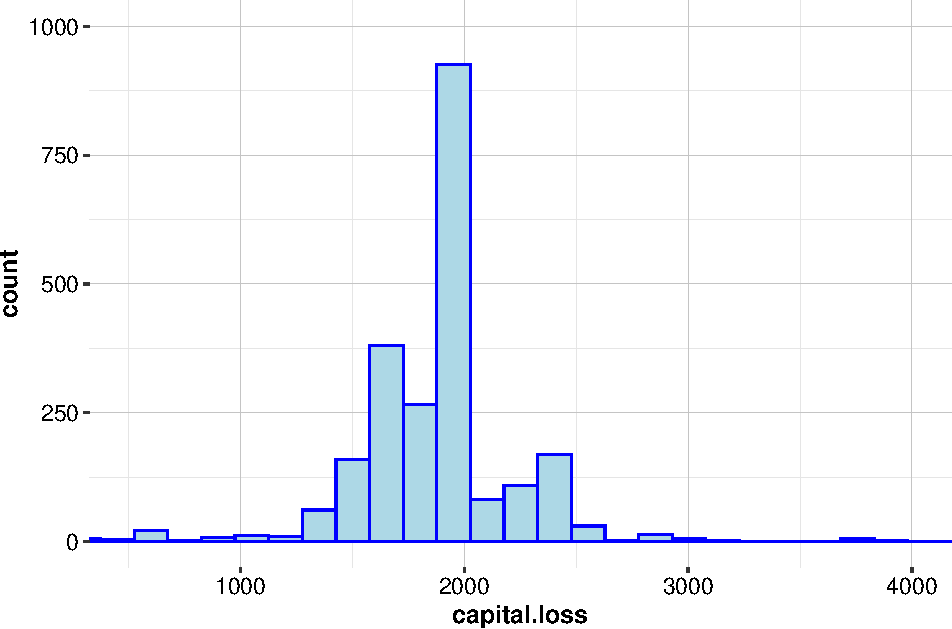
\includegraphics[width=0.7\linewidth]{data-preparation_files/figure-latex/unnamed-chunk-28-1} \end{center}

\begin{lstlisting}[language=R]
ggplot(data = subset(adult, capital.loss > 0)) +
     geom_boxplot(aes(y = capital.loss)) 
\end{lstlisting}

\begin{center}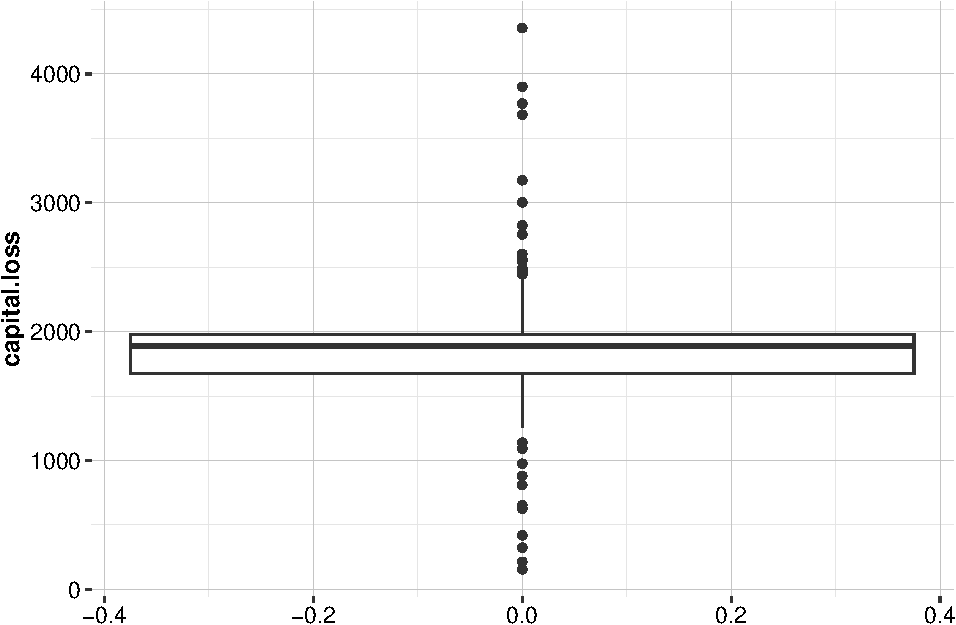
\includegraphics[width=0.7\linewidth]{data-preparation_files/figure-latex/unnamed-chunk-29-1} \end{center}

Key takeaways from these refined plots:

\begin{itemize}
\tightlist
\item
  The majority of nonzero values are below 500, with a small number extending beyond 4,000.\\
\item
  The distribution of nonzero values is approximately symmetric, suggesting that while there are extreme values, they follow a structured pattern rather than random anomalies.
\end{itemize}

\subsubsection*{Handling Outliers}\label{handling-outliers}
\addcontentsline{toc}{subsubsection}{Handling Outliers}

Although \passthrough{\lstinline!capital.loss!} contains many high values, these do not appear to be erroneous. Instead, they reflect genuine cases within the dataset. Since these values provide meaningful information about particular individuals, we retain them rather than applying transformations or removals.

However, if model performance is significantly affected by these extreme values, we might consider:

\begin{enumerate}
\def\labelenumi{\arabic{enumi}.}
\tightlist
\item
  \emph{Winsorization}: Capping values at a reasonable percentile (e.g., the 95th percentile).\\
\item
  \emph{Log Transformation}: Applying a log transformation to reduce skewness.\\
\item
  \emph{Creating a Binary Indicator}: Introducing a new variable indicating whether a capital loss occurred (\passthrough{\lstinline!capital.loss > 0!}).
\end{enumerate}

Next, we perform a similar outlier analysis for the \passthrough{\lstinline!capital.gain!} variable. See the exercises below for a guided approach.

\section{Exercises}\label{exercises-1}

This section provides hands-on exercises to reinforce the key concepts covered in this chapter. These questions include theoretical, exploratory, and practical challenges related to data types, outliers, encoding techniques, and feature engineering.

\subsection*{Understanding Data Types}\label{understanding-data-types}
\addcontentsline{toc}{subsection}{Understanding Data Types}

\begin{enumerate}
\def\labelenumi{\arabic{enumi}.}
\tightlist
\item
  What is the difference between continuous and discrete numerical variables? Provide an example of each from real-world data.\\
\item
  How do ordinal categorical variables differ from nominal categorical variables? Give an example for both.
\end{enumerate}

\subsection*{Exploring the diamonds Dataset}\label{exploring-the-diamonds-dataset}
\addcontentsline{toc}{subsection}{Exploring the diamonds Dataset}

\begin{enumerate}
\def\labelenumi{\arabic{enumi}.}
\setcounter{enumi}{2}
\tightlist
\item
  Report the summary statistics for the diamonds dataset using the \passthrough{\lstinline!summary()!} function. What insights can you derive from the output?\\
\item
  In the diamonds dataset, which variables are nominal, ordinal, and numerical? List them accordingly.
\end{enumerate}

\subsection*{Detecting and Handling Outliers}\label{detecting-and-handling-outliers}
\addcontentsline{toc}{subsection}{Detecting and Handling Outliers}

\begin{enumerate}
\def\labelenumi{\arabic{enumi}.}
\setcounter{enumi}{4}
\tightlist
\item
  Identify outliers in the variable \passthrough{\lstinline!x!}. If any exist, handle them appropriately. Follow the same approach as in Section \ref{Data-pre-outliers} for the \passthrough{\lstinline!y!} variable in the diamonds dataset.\\
\item
  Repeat the outlier detection process for the variable \passthrough{\lstinline!z!}. If necessary, apply transformations or filtering techniques.\\
\item
  Check for outliers in the \passthrough{\lstinline!depth!} variable. What method would you use to detect and handle them?
\end{enumerate}

\subsection*{Encoding Categorical Variables}\label{encoding-categorical-variables-1}
\addcontentsline{toc}{subsection}{Encoding Categorical Variables}

\begin{enumerate}
\def\labelenumi{\arabic{enumi}.}
\setcounter{enumi}{7}
\tightlist
\item
  The \passthrough{\lstinline!cut!} variable in the diamonds dataset is ordinal. How can we encode it properly using ordinal encoding?\\
\item
  The \passthrough{\lstinline!color!} variable in the diamonds dataset is nominal. How can we encode it using one-hot encoding?
\end{enumerate}

\subsection*{Analyzing the Adult Dataset}\label{analyzing-the-adult-dataset}
\addcontentsline{toc}{subsection}{Analyzing the Adult Dataset}

\begin{enumerate}
\def\labelenumi{\arabic{enumi}.}
\setcounter{enumi}{9}
\tightlist
\item
  Load the Adult dataset from the \textbf{liver} package and examine its structure. Identify the categorical variables and classify them as nominal or ordinal.\\
\item
  Compute the proportion of individuals who earn more than 50K (\passthrough{\lstinline!>50K!}). What does this distribution tell you about income levels in this dataset?\\
\item
  For the Adult dataset, generate the summary statistics, boxplot, and histogram for the variable \passthrough{\lstinline!capital.gain!}. What do you observe?\\
\item
  Based on the visualizations from the previous question, are there outliers in the \passthrough{\lstinline!capital.gain!} variable? If so, suggest a strategy to handle them.
\end{enumerate}

\subsection*{Feature Engineering Challenge}\label{feature-engineering-challenge}
\addcontentsline{toc}{subsection}{Feature Engineering Challenge}

\begin{enumerate}
\def\labelenumi{\arabic{enumi}.}
\setcounter{enumi}{13}
\tightlist
\item
  Create a new categorical variable \passthrough{\lstinline!Age\_Group!} in the Adult dataset, grouping ages into:\\
\end{enumerate}

\begin{itemize}
\tightlist
\item
  Young (≤30 years old)\\
\item
  Middle-aged (31-50 years old)\\
\item
  Senior (\textgreater50 years old)\\
  Use the \passthrough{\lstinline!cut()!} function to implement this transformation.
\end{itemize}

\begin{enumerate}
\def\labelenumi{\arabic{enumi}.}
\setcounter{enumi}{14}
\tightlist
\item
  Compute the mean \passthrough{\lstinline!capital.gain!} for each \passthrough{\lstinline!Age\_Group!}. What insights do you gain about income levels across different age groups?
\end{enumerate}

\subsection*{Advanced Data Preparation Challenges}\label{advanced-data-preparation-challenges}
\addcontentsline{toc}{subsection}{Advanced Data Preparation Challenges}

\begin{enumerate}
\def\labelenumi{\arabic{enumi}.}
\setcounter{enumi}{15}
\item
  In the Adult dataset, the \passthrough{\lstinline!education!} variable contains 16 distinct levels. Reduce these categories into broader groups such as ``No Diploma,'' ``High School Graduate,'' ``Some College,'' and ``Postgraduate.'' Implement this transformation using the \passthrough{\lstinline!fct\_collapse()!} function.
\item
  The \passthrough{\lstinline!capital.gain!} and \passthrough{\lstinline!capital.loss!} variables represent financial assets. Create a new variable \passthrough{\lstinline!net.capital!} that computes the difference between \passthrough{\lstinline!capital.gain!} and \passthrough{\lstinline!capital.loss!}. Analyze its distribution.
\item
  Perform Min-Max scaling on the numerical variables in the Adult dataset (\passthrough{\lstinline!age!}, \passthrough{\lstinline!capital.gain!}, \passthrough{\lstinline!capital.loss!}, \passthrough{\lstinline!hours.per.week!}). Use the \passthrough{\lstinline!mutate()!} function to apply this transformation.
\item
  Perform Z-score normalization on the same set of numerical variables. Compare the results with Min-Max scaling. In what scenarios would one approach be preferable over the other?
\item
  Construct a logistic regression model to predict whether an individual earns more than 50K (\passthrough{\lstinline!>50K!}) based on selected numerical features (\passthrough{\lstinline!age!}, \passthrough{\lstinline!education.num!}, \passthrough{\lstinline!hours.per.week!}). Preprocess the data accordingly and interpret the coefficients of the model.
\end{enumerate}

\chapter{Exploratory Data Analysis}\label{chapter-EDA}

Exploratory Data Analysis (EDA) is a fundamental step in data science that helps uncover insights, detect patterns, and understand relationships within a dataset. Before applying statistical models or machine learning algorithms, it is essential to explore and visualize data to identify inconsistencies, anomalies, and potential predictors. EDA provides a structured yet flexible approach to data exploration, allowing data scientists to make informed decisions before proceeding with modeling.

EDA is an iterative process rather than a rigid sequence of steps. It encourages curiosity and adaptability, as different datasets may present unique challenges or insights. Some exploratory paths may lead to inconclusive findings, while others uncover valuable patterns that shape the direction of analysis. As familiarity with the data increases, analysts can refine their focus, identifying the most relevant features and variables for modeling.

The primary goal of EDA is to explore and summarize data rather than to perform hypothesis testing or confirm specific relationships. By using summary statistics, visualizations, and preliminary correlation analysis, EDA provides a foundational understanding of the dataset. However, these insights remain preliminary and require further validation through statistical testing or predictive modeling. Recognizing this distinction ensures that exploratory findings are interpreted cautiously and do not lead to premature conclusions.

Another key consideration in EDA is balancing statistical significance with practical relevance. Large datasets often reveal statistically significant relationships that may lack meaningful real-world implications. For example, a weak correlation between customer engagement and churn might be statistically significant yet offer little actionable insight for business decision-making. EDA encourages analysts to integrate domain expertise and practical considerations when interpreting patterns in data.

EDA also plays a crucial role in data cleaning and preparation. Missing values, inconsistencies, and outliers often become apparent during exploration, requiring careful handling to ensure data quality. While data cleaning is a distinct process, it is closely linked to EDA, as identifying and resolving data issues early helps establish a solid foundation for further analysis and modeling.

Selecting appropriate tools and techniques for EDA depends on the nature of the dataset and the specific analytical questions. Histograms and box plots help visualize distributions, while scatter plots and correlation matrices assess relationships between variables. The following sections will demonstrate these techniques through practical applications, including an in-depth analysis of the churn dataset to illustrate how EDA can uncover patterns relevant to customer retention.

The key objectives of EDA are:

\begin{enumerate}
\def\labelenumi{\arabic{enumi}.}
\tightlist
\item
  \textbf{Understanding the structure of the data} -- Determine data types, variable ranges, the number of observations, and the presence of missing values or anomalies.\\
\item
  \textbf{Analyzing individual variable distributions} -- Examine numerical and categorical variables to assess their distribution, central tendency, and spread.\\
\item
  \textbf{Exploring relationships between variables} -- Identify correlations, dependencies, or interactions that may influence predictive modeling.\\
\item
  \textbf{Detecting patterns and outliers} -- Identify unusual data points and assess whether they result from data errors or represent meaningful trends.
\end{enumerate}

These objectives ensure a comprehensive understanding of the dataset, forming a strong foundation for subsequent modeling and analysis.

\section{Guiding Questions for EDA}\label{guiding-questions-for-eda}

Exploratory data analysis is most effective when structured around key questions that help uncover meaningful patterns and relationships. These questions generally fall into two broad categories: univariate and multivariate analysis.

Univariate analysis examines individual variables to assess their distributions, central tendencies, variability, and potential data quality issues such as missing values or outliers. Typical univariate questions include:

\begin{itemize}
\tightlist
\item
  What is the distribution of the target variable?\\
\item
  How are numerical variables, such as income or age, distributed?\\
\item
  Are there missing values, and how are they distributed across the dataset?
\end{itemize}

This analysis helps detect skewness, irregularities, and unexpected patterns that may impact later modeling. Common tools for univariate analysis include histograms, box plots, and summary statistics such as the mean, median, quartiles, and standard deviation.

Multivariate analysis explores relationships between two or more variables, identifying dependencies, interactions, or correlations that could influence predictive modeling. Key multivariate questions include:

\begin{itemize}
\tightlist
\item
  How does the target variable relate to predictor variables?\\
\item
  Are some predictors highly correlated, suggesting potential multicollinearity?\\
\item
  How do categorical and numerical variables interact?
\end{itemize}

To analyze these relationships, data scientists commonly use scatter plots, correlation matrices, and pairwise comparisons, which help visualize dependencies between variables and guide feature selection.

A common challenge in EDA is choosing the most appropriate visualization or statistical summary for a given analysis. The selection depends on both the type of data and the insight being sought. The table below provides a structured guide to selecting the most effective tools for various exploratory tasks:

\begin{table}

\caption{\label{tab:EDA-table-tools}EDA Tool Selection Guide.}
\centering
\begin{tabular}[t]{lll}
\toprule
EDA.Objective & Data.Type & Recommended.Tools\\
\midrule
Understand the distribution of a variable & Numerical (continuous/discrete) & Histogram, box plot, density plot, summary statistics\\
Examine a categorical variable's distribution & Categorical & Bar chart, frequency table\\
Identify outliers & Numerical & Box plot, histogram, Z-score analysis\\
Detect missing values & Any & Heatmap, summary statistics, missing data patterns\\
Analyze the relationship between two numerical variables & Numerical \& numerical & Scatter plot, correlation coefficient, regression line\\
\addlinespace
Compare a numerical variable across categories & Categorical \& numerical & Box plot, violin plot, grouped bar chart\\
Explore interactions between two categorical variables & Categorical \& categorical & Stacked bar chart, mosaic plot, contingency table\\
Assess correlation among multiple numerical variables & Multiple numerical & Correlation matrix, pair plot (scatterplot matrix)\\
Investigate complex multivariate relationships & Multiple variables & Facet grid, parallel coordinates, principal component analysis (PCA)\\
\bottomrule
\end{tabular}
\end{table}

By systematically addressing these univariate and multivariate questions with appropriate EDA techniques, we gain a deeper understanding of the dataset's structure and key patterns. This process not only improves data quality but also provides valuable insights that inform subsequent modeling and decision-making.

\section{EDA as Data Storytelling}\label{eda-as-data-storytelling}

Exploratory Data Analysis is more than just a technical step; it is a way to uncover and communicate meaningful insights from data. Beyond summarizing numbers and visualizing patterns, EDA helps shape the narrative hidden within the data. Effective data storytelling integrates data, visuals, and context, making findings more accessible and actionable. Whether communicating with data scientists, business professionals, or decision-makers, presenting insights clearly is essential.

While summary statistics provide an overview, visualizations reveal patterns, relationships, and anomalies that might otherwise go unnoticed. Different types of visualizations serve distinct purposes. Scatter plots and correlation matrices highlight relationships between numerical variables, while histograms and box plots illustrate distributions and potential skewness. Categorical data is best explored with bar charts or stacked visualizations, allowing comparisons across different groups. Choosing the right visualization ensures insights are both accurate and intuitive.

A strong narrative connects data insights with real-world significance. Rather than simply presenting a correlation coefficient or a distribution plot, a well-structured EDA report explains why a pattern matters and how it informs decision-making. Instead of stating that customers with high daytime phone usage have a higher churn rate, it is more impactful to provide context:

\emph{``Customers with extensive daytime usage are significantly more likely to churn, possibly due to pricing concerns or dissatisfaction with service quality. Targeted retention strategies, such as customized discounts or flexible pricing plans, may help mitigate this risk.''}

This approach goes beyond numerical reporting, framing insights as actionable strategies.

Data storytelling is widely used in business, scientific research, and journalism. Consider the following examples that illustrate how visual storytelling enhances understanding.

One example comes from climate science. Figure \ref{fig:EDA-fig-1} presents global mean surface temperature changes over the Common Era, highlighting long-term warming trends. Adapted from \citet{neukom2019no}, this visualization provides a historical perspective on climate change, illustrating temperature anomalies over time.

\begin{figure}

{\centering 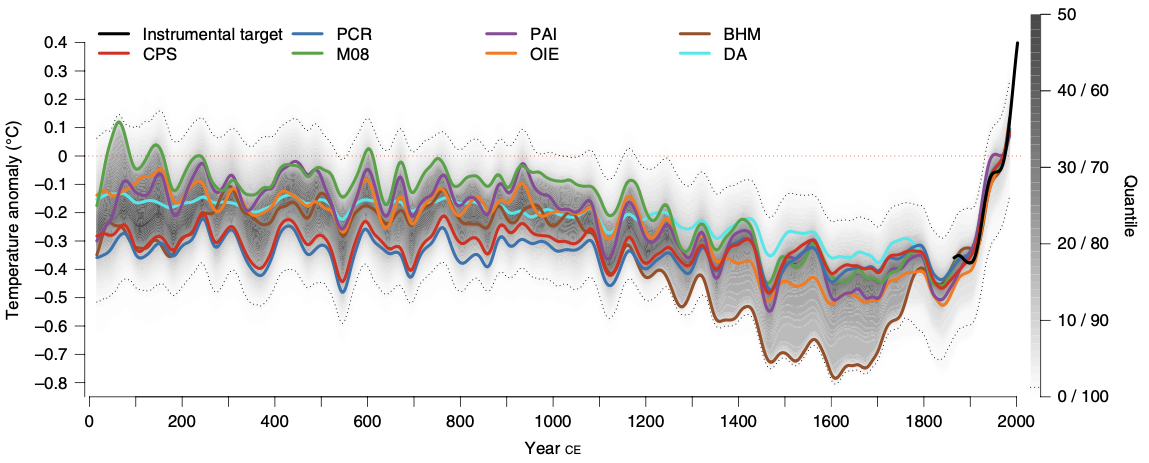
\includegraphics[width=1\linewidth]{images/EDA_fig_1} 

}

\caption{Global mean surface temperature history over the Common Era. Temperature anomalies with respect to 1961–1990 CE. The colored lines represent 30-year low-pass-filtered ensemble medians for different reconstruction methods.}\label{fig:EDA-fig-1}
\end{figure}

Another example focuses on global health and demographics. Figure \ref{fig:EDA-fig-2} illustrates the relationship between fertility rate and life expectancy across world regions from 1960 to 2015. Adapted from Hans Rosling's TED Talk \href{https://www.ted.com/talks/hans_rosling_new_insights_on_poverty}{``New insights on poverty''}, this visualization effectively conveys trends in population health and economic development over time.

These examples highlight how well-designed visualizations can make complex data more accessible and engaging.

When conducting EDA, it is essential to consider the broader narrative. Instead of just reporting statistical results, think about what a trend reveals, why it is relevant, and how it can inform decision-making. Integrating storytelling techniques ensures that EDA serves not only as a data exploration step but also as a communication tool that connects technical analysis with practical application.

\section{\texorpdfstring{EDA in Practice: The \emph{Churn} Dataset}{EDA in Practice: The Churn Dataset}}\label{EDA-sec-churn}

To illustrate the exploratory data analysis process, we will use the \emph{churn} dataset, which contains information about customer behavior, including whether a customer has churned (i.e., left the service) and various demographic and behavioral attributes.

EDA will help us understand this dataset by identifying patterns related to customer churn, determining which features influence retention, and establishing a structured approach for predictive modeling. By examining summary statistics and visualizations, we can extract meaningful insights before moving on to machine learning techniques in later chapters.

\subsection*{Problem Understanding}\label{problem-understanding-1}
\addcontentsline{toc}{subsection}{Problem Understanding}

Companies seek to minimize customer churn by identifying factors that influence customer decisions. Key business questions include:

\begin{itemize}
\tightlist
\item
  \textbf{Why} are customers leaving?\\
\item
  \textbf{What} are the primary factors contributing to churn?\\
\item
  \textbf{How} can we take action to improve retention?
\end{itemize}

EDA helps answer these questions by uncovering trends and patterns in customer behavior. In Chapter \ref{chapter-knn}, we will build a predictive model to identify customers likely to churn. Before doing so, it is essential to explore the data and understand its structure.

\subsection*{Data Understanding}\label{data-understanding}
\addcontentsline{toc}{subsection}{Data Understanding}

The \emph{churn} dataset comes from IBM Sample Data Sets and contains 5000 customer records across 20 variables. This dataset is available in the \textbf{liver} package. The target variable, \passthrough{\lstinline!churn!}, indicates whether a customer has left the company. The dataset includes a mix of categorical and numerical variables:

\begin{itemize}
\tightlist
\item
  \passthrough{\lstinline!state!} : Categorical, state in the U.S. (51 states + D.C.).
\item
  \passthrough{\lstinline!area.code!} : Categorical, area code assigned to the customer.
\item
  \passthrough{\lstinline!account.length!} : Numerical (discrete), duration of account activity (days).
\item
  \passthrough{\lstinline!voice.plan!} : Categorical (binary), subscription to a voice mail plan (yes/no).
\item
  \passthrough{\lstinline!voice.messages!} : Numerical (discrete), number of voice mail messages.
\item
  \passthrough{\lstinline!intl.plan!} : Categorical (binary), subscription to an international calling plan (yes/no).
\item
  \passthrough{\lstinline!intl.mins!} : Numerical (continuous), total international call minutes.
\item
  \passthrough{\lstinline!intl.calls!} : Numerical (discrete), total international calls made.
\item
  \passthrough{\lstinline!intl.charge!} : Numerical (continuous), total international call charges.
\item
  \passthrough{\lstinline!day.mins!} : Numerical (continuous), total daytime call minutes.
\item
  \passthrough{\lstinline!day.calls!} : Numerical (discrete), total daytime calls made.
\item
  \passthrough{\lstinline!day.charge!} : Numerical (continuous), total daytime call charges.
\item
  \passthrough{\lstinline!eve.mins!} : Numerical (continuous), total evening call minutes.
\item
  \passthrough{\lstinline!eve.calls!} : Numerical (discrete), total evening calls made.
\item
  \passthrough{\lstinline!eve.charge!} : Numerical (continuous), total evening call charges.
\item
  \passthrough{\lstinline!night.mins!} : Numerical (continuous), total nighttime call minutes.
\item
  \passthrough{\lstinline!night.calls!} : Numerical (discrete), total nighttime calls made.
\item
  \passthrough{\lstinline!night.charge!} : Numerical (continuous), total nighttime call charges.
\item
  \passthrough{\lstinline!customer.calls!} : Numerical (discrete), number of customer service calls made.
\item
  \passthrough{\lstinline!churn!} : Categorical (binary), indicates whether the customer churned (yes/no).
\end{itemize}

To use this dataset, we first load the \textbf{liver} package and then import the dataset into \textbf{R}:

\begin{lstlisting}[language=R]
library(liver)
data(churn)  
\end{lstlisting}

To examine the structure of the dataset, we use:

\begin{lstlisting}[language=R]
str(churn)  
   'data.frame':    5000 obs. of  20 variables:
    $ state         : Factor w/ 51 levels "AK","AL","AR",..: 17 36 32 36 37 2 20 25 19 50 ...
    $ area.code     : Factor w/ 3 levels "area_code_408",..: 2 2 2 1 2 3 3 2 1 2 ...
    $ account.length: int  128 107 137 84 75 118 121 147 117 141 ...
    $ voice.plan    : Factor w/ 2 levels "yes","no": 1 1 2 2 2 2 1 2 2 1 ...
    $ voice.messages: int  25 26 0 0 0 0 24 0 0 37 ...
    $ intl.plan     : Factor w/ 2 levels "yes","no": 2 2 2 1 1 1 2 1 2 1 ...
    $ intl.mins     : num  10 13.7 12.2 6.6 10.1 6.3 7.5 7.1 8.7 11.2 ...
    $ intl.calls    : int  3 3 5 7 3 6 7 6 4 5 ...
    $ intl.charge   : num  2.7 3.7 3.29 1.78 2.73 1.7 2.03 1.92 2.35 3.02 ...
    $ day.mins      : num  265 162 243 299 167 ...
    $ day.calls     : int  110 123 114 71 113 98 88 79 97 84 ...
    $ day.charge    : num  45.1 27.5 41.4 50.9 28.3 ...
    $ eve.mins      : num  197.4 195.5 121.2 61.9 148.3 ...
    $ eve.calls     : int  99 103 110 88 122 101 108 94 80 111 ...
    $ eve.charge    : num  16.78 16.62 10.3 5.26 12.61 ...
    $ night.mins    : num  245 254 163 197 187 ...
    $ night.calls   : int  91 103 104 89 121 118 118 96 90 97 ...
    $ night.charge  : num  11.01 11.45 7.32 8.86 8.41 ...
    $ customer.calls: int  1 1 0 2 3 0 3 0 1 0 ...
    $ churn         : Factor w/ 2 levels "yes","no": 2 2 2 2 2 2 2 2 2 2 ...
\end{lstlisting}

This command reveals that the dataset is stored as a \passthrough{\lstinline!data.frame!} with 5000 observations and 20 variables. The target variable, \passthrough{\lstinline!churn!}, categorizes whether a customer has left the service.

To summarize the dataset, we use:

\begin{lstlisting}[language=R]
summary(churn)
        state              area.code    account.length  voice.plan
    WV     : 158   area_code_408:1259   Min.   :  1.0   yes:1323  
    MN     : 125   area_code_415:2495   1st Qu.: 73.0   no :3677  
    AL     : 124   area_code_510:1246   Median :100.0             
    ID     : 119                        Mean   :100.3             
    VA     : 118                        3rd Qu.:127.0             
    OH     : 116                        Max.   :243.0             
    (Other):4240                                                  
    voice.messages   intl.plan    intl.mins       intl.calls      intl.charge   
    Min.   : 0.000   yes: 473   Min.   : 0.00   Min.   : 0.000   Min.   :0.000  
    1st Qu.: 0.000   no :4527   1st Qu.: 8.50   1st Qu.: 3.000   1st Qu.:2.300  
    Median : 0.000              Median :10.30   Median : 4.000   Median :2.780  
    Mean   : 7.755              Mean   :10.26   Mean   : 4.435   Mean   :2.771  
    3rd Qu.:17.000              3rd Qu.:12.00   3rd Qu.: 6.000   3rd Qu.:3.240  
    Max.   :52.000              Max.   :20.00   Max.   :20.000   Max.   :5.400  
                                                                                
       day.mins       day.calls     day.charge       eve.mins       eve.calls    
    Min.   :  0.0   Min.   :  0   Min.   : 0.00   Min.   :  0.0   Min.   :  0.0  
    1st Qu.:143.7   1st Qu.: 87   1st Qu.:24.43   1st Qu.:166.4   1st Qu.: 87.0  
    Median :180.1   Median :100   Median :30.62   Median :201.0   Median :100.0  
    Mean   :180.3   Mean   :100   Mean   :30.65   Mean   :200.6   Mean   :100.2  
    3rd Qu.:216.2   3rd Qu.:113   3rd Qu.:36.75   3rd Qu.:234.1   3rd Qu.:114.0  
    Max.   :351.5   Max.   :165   Max.   :59.76   Max.   :363.7   Max.   :170.0  
                                                                                 
      eve.charge      night.mins     night.calls      night.charge   
    Min.   : 0.00   Min.   :  0.0   Min.   :  0.00   Min.   : 0.000  
    1st Qu.:14.14   1st Qu.:166.9   1st Qu.: 87.00   1st Qu.: 7.510  
    Median :17.09   Median :200.4   Median :100.00   Median : 9.020  
    Mean   :17.05   Mean   :200.4   Mean   : 99.92   Mean   : 9.018  
    3rd Qu.:19.90   3rd Qu.:234.7   3rd Qu.:113.00   3rd Qu.:10.560  
    Max.   :30.91   Max.   :395.0   Max.   :175.00   Max.   :17.770  
                                                                     
    customer.calls churn     
    Min.   :0.00   yes: 707  
    1st Qu.:1.00   no :4293  
    Median :1.00             
    Mean   :1.57             
    3rd Qu.:2.00             
    Max.   :9.00             
   
\end{lstlisting}

This function provides a high-level overview of all variables, including their distributions and any potential missing values. The dataset is clean and ready for exploratory data analysis. In the next sections, we will explore its structure using visualizations and statistical summaries. This will help us identify key variables influencing churn and ensure the dataset is well-prepared for predictive modeling.

One notable observation is that there are 51 unique states represented in the dataset, yet only 3 unique area codes. This suggests that area codes do not correspond directly to state locations, which is worth investigating further.

\section{Investigating Categorical Variables}\label{chapter-EDA-categorical}

Categorical variables represent discrete values such as labels, names, or binary indicators. In the \emph{churn} dataset, key categorical features include \passthrough{\lstinline!state!}, \passthrough{\lstinline!area.code!}, \passthrough{\lstinline!voice.plan!}, and \passthrough{\lstinline!intl.plan!}. Understanding their distributions and relationships with the target variable helps uncover trends that may influence customer retention.

To begin, we examine the distribution of the target variable \passthrough{\lstinline!churn!} to determine whether the dataset is balanced:

\begin{lstlisting}[language=R]
ggplot(data = churn, aes(x = churn, label = scales::percent(prop.table(stat(count))))) +
  geom_bar(fill = c("palevioletred1", "darkseagreen1")) + 
  geom_text(stat = 'count', vjust = 0.2, size = 6)
\end{lstlisting}

\begin{center}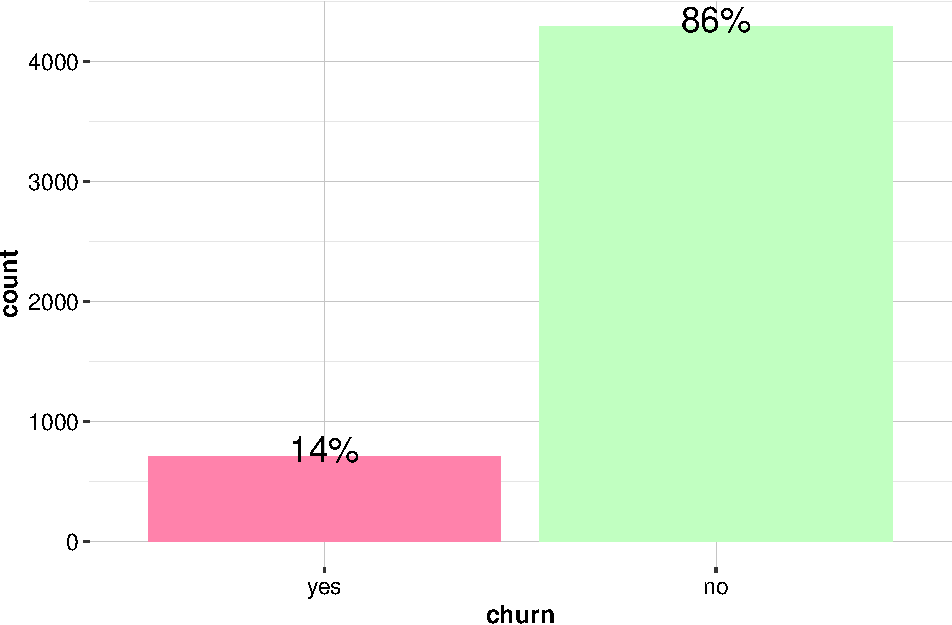
\includegraphics[width=0.7\linewidth]{EDA_files/figure-latex/unnamed-chunk-4-1} \end{center}

The bar plot reveals that the dataset is imbalanced, with more customers staying (\passthrough{\lstinline!churn = "no"!}) than leaving (\passthrough{\lstinline!churn = "yes"!}). The proportion of churners is approximately 1.4 percent, while the proportion of non-churners is 8.6 percent. Since imbalanced data can impact predictive modeling, understanding churn patterns is essential for improving retention strategies.

\subsection*{Relationship Between Churn and Subscription Plans}\label{relationship-between-churn-and-subscription-plans}
\addcontentsline{toc}{subsection}{Relationship Between Churn and Subscription Plans}

We first analyze \passthrough{\lstinline!intl.plan!}, which indicates whether a customer has an international calling plan. As a binary variable, it allows for a straightforward comparison of churn rates between subscribed and non-subscribed customers.

\begin{lstlisting}[language=R]
ggplot(data = churn) + 
  geom_bar(aes(x = intl.plan, fill = churn)) +
  scale_fill_manual(values = c("palevioletred1", "darkseagreen1")) 

ggplot(data = churn) + 
  geom_bar(aes(x = intl.plan, fill = churn), position = "fill") +
  scale_fill_manual(values = c("palevioletred1", "darkseagreen1")) 
\end{lstlisting}

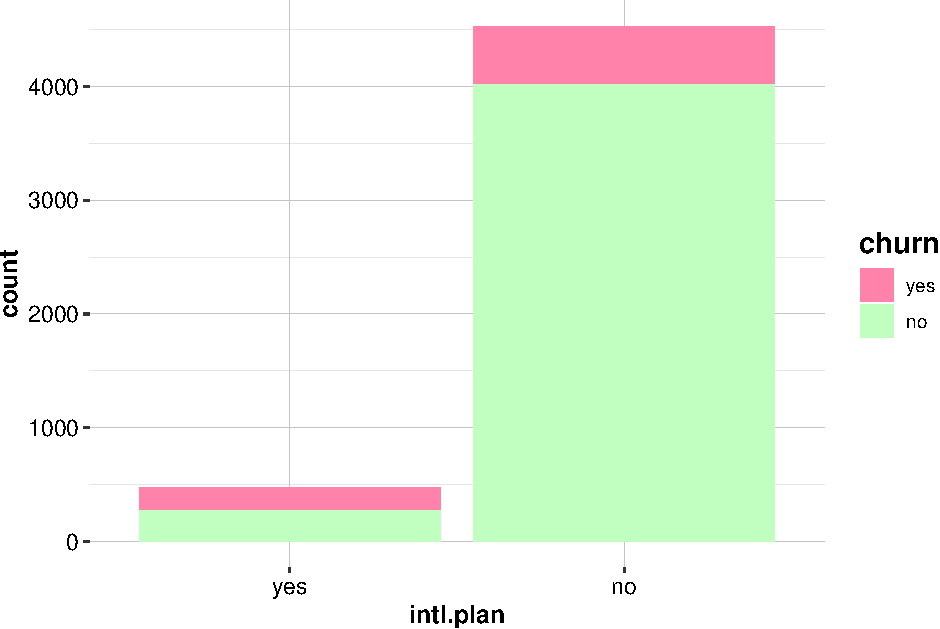
\includegraphics[width=0.5\linewidth]{EDA_files/figure-latex/unnamed-chunk-5-1} 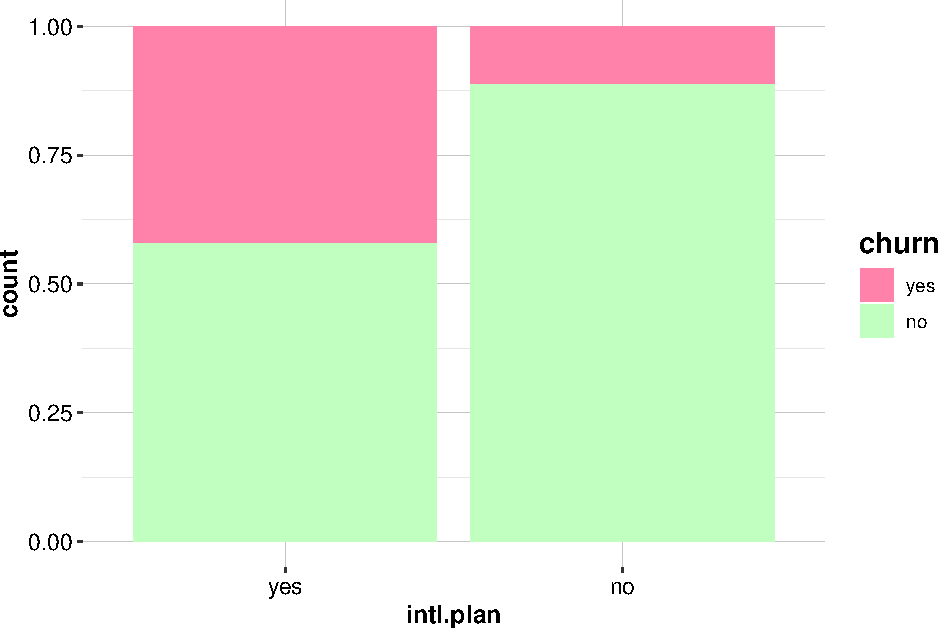
\includegraphics[width=0.5\linewidth]{EDA_files/figure-latex/unnamed-chunk-5-2}

The first plot (left) compares the raw counts of churners and non-churners among customers with and without an international plan. The second plot (right) normalizes the proportions, revealing that customers with an international plan have a significantly higher churn rate.

To quantify this relationship, we generate a contingency table:

\begin{lstlisting}[language=R]
addmargins(table(churn$churn, churn$intl.plan, 
                 dnn = c("Churn", "International Plan")))
        International Plan
   Churn  yes   no  Sum
     yes  199  508  707
     no   274 4019 4293
     Sum  473 4527 5000
\end{lstlisting}

The results confirm that churn is more prevalent among customers subscribed to an international plan. This suggests that international service offerings may not be meeting customer expectations, leading to higher attrition. Companies may need to investigate whether pricing, service quality, or competition is influencing this trend.

\subsection*{Relationship Between Churn and Voice Mail Plan}\label{relationship-between-churn-and-voice-mail-plan}
\addcontentsline{toc}{subsection}{Relationship Between Churn and Voice Mail Plan}

Next, we examine \passthrough{\lstinline!voice.plan!}, which indicates whether a customer has subscribed to a voice mail plan.

\begin{lstlisting}[language=R]
ggplot(data = churn) + 
  geom_bar(aes(x = voice.plan, fill = churn)) +
  scale_fill_manual(values = c("palevioletred1", "darkseagreen1")) 

ggplot(data = churn) + 
  geom_bar(aes(x = voice.plan, fill = churn), position = "fill") +
  scale_fill_manual(values = c("palevioletred1", "darkseagreen1")) 
\end{lstlisting}

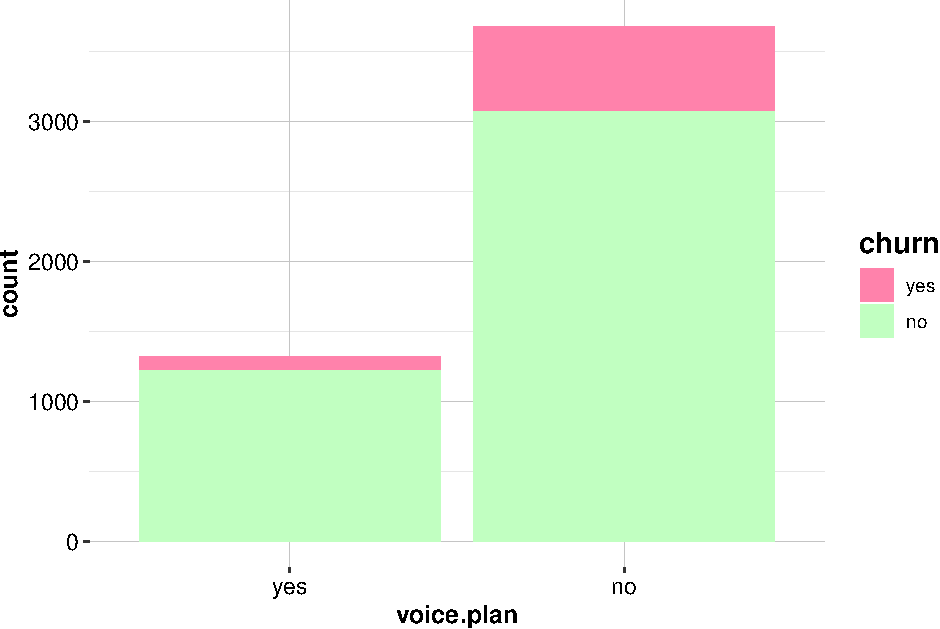
\includegraphics[width=0.5\linewidth]{EDA_files/figure-latex/unnamed-chunk-7-1} 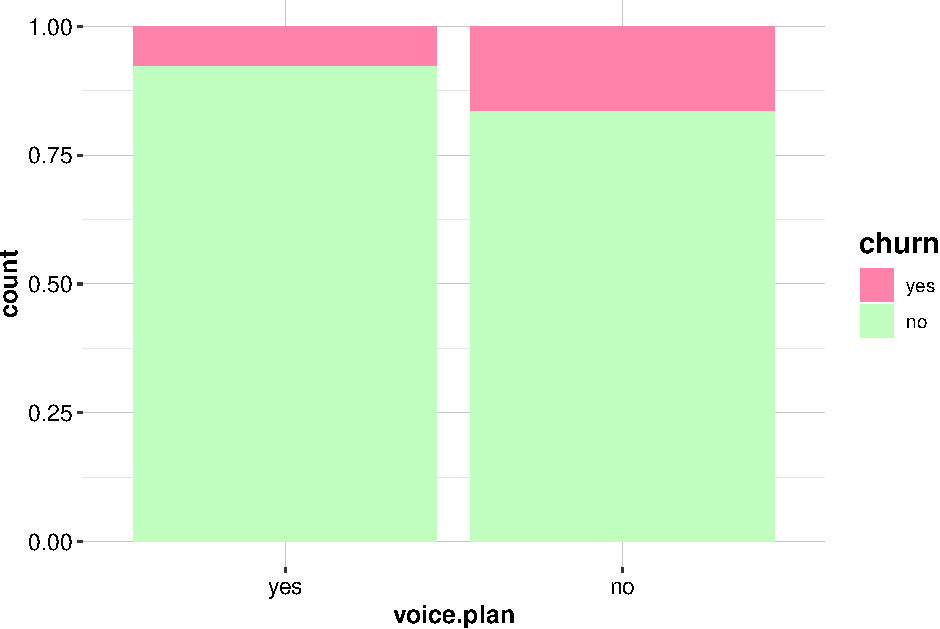
\includegraphics[width=0.5\linewidth]{EDA_files/figure-latex/unnamed-chunk-7-2}

Customers without a voice mail plan appear to churn at a slightly higher rate. This is confirmed using a contingency table:

\begin{lstlisting}[language=R]
addmargins(table(churn$churn, churn$voice.plan, dnn = c("Churn", "Voice Mail Plan")))
        Voice Mail Plan
   Churn  yes   no  Sum
     yes  102  605  707
     no  1221 3072 4293
     Sum 1323 3677 5000
\end{lstlisting}

While the difference is less pronounced than for \passthrough{\lstinline!intl.plan!}, it suggests that customers who actively use voice mail services may be more engaged and therefore less likely to leave.

\subsubsection*{Key Insights}\label{key-insights}
\addcontentsline{toc}{subsubsection}{Key Insights}

\begin{itemize}
\tightlist
\item
  Customers subscribed to an international plan have a \textbf{significantly higher} churn rate, indicating a potential issue with service expectations, pricing, or customer satisfaction. This variable is likely to be an important predictor in churn models.
\item
  Customers with a voice mail plan have a \textbf{slightly lower} churn rate, suggesting that engagement with additional services may contribute to customer retention.
\item
  These insights highlight the importance of investigating product-specific factors when analyzing churn, as different subscription plans may have varying impacts on customer behavior.
\end{itemize}

By exploring categorical variables in this way, we uncover actionable insights that can inform both predictive modeling and business decisions aimed at reducing customer churn. In the next section, we will examine numerical variables to further refine our understanding of customer behavior.

\section{Investigating Numerical Variables}\label{EDA-sec-numeric}

We now turn to numerical variables in the churn dataset, examining their distributions and relationships with the target variable. Summary statistics provide an initial understanding, but visualizations such as histograms, box plots, and density plots help reveal patterns and potential predictors of churn.

\subsection*{Customer Service Calls and Churn}\label{customer-service-calls-and-churn}
\addcontentsline{toc}{subsection}{Customer Service Calls and Churn}

The variable \passthrough{\lstinline!customer.calls!} represents the number of calls a customer makes to customer service. Since this is a discrete numerical variable, we use a histogram to examine its distribution:

\begin{lstlisting}[language=R]
ggplot(data = churn) +
  geom_histogram(aes(x = customer.calls), 
                 bins = 10, fill = "skyblue", color = "black")
\end{lstlisting}

\begin{center}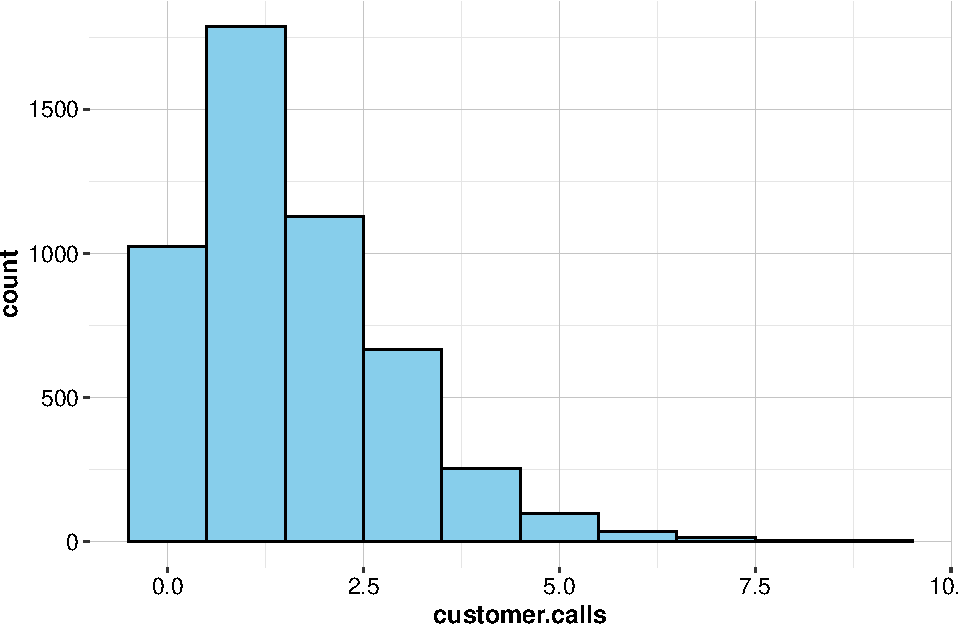
\includegraphics[width=0.7\linewidth]{EDA_files/figure-latex/unnamed-chunk-9-1} \end{center}

The histogram shows that most customers make only a few service calls, while a smaller group contacts customer service frequently. The right-skewed distribution suggests that a few customers make an unusually high number of calls, potentially signaling dissatisfaction.

To further investigate, we overlay churn status:

\begin{lstlisting}[language=R]
ggplot(data = churn) +
  geom_histogram(aes(x = customer.calls, fill = churn), position = "stack") +
  scale_fill_manual(values = c("palevioletred1", "darkseagreen1")) 
  
ggplot(data = churn) +
  geom_histogram(aes(x = customer.calls, fill = churn), position = "fill") +
  scale_fill_manual(values = c("palevioletred1", "darkseagreen1")) 
\end{lstlisting}

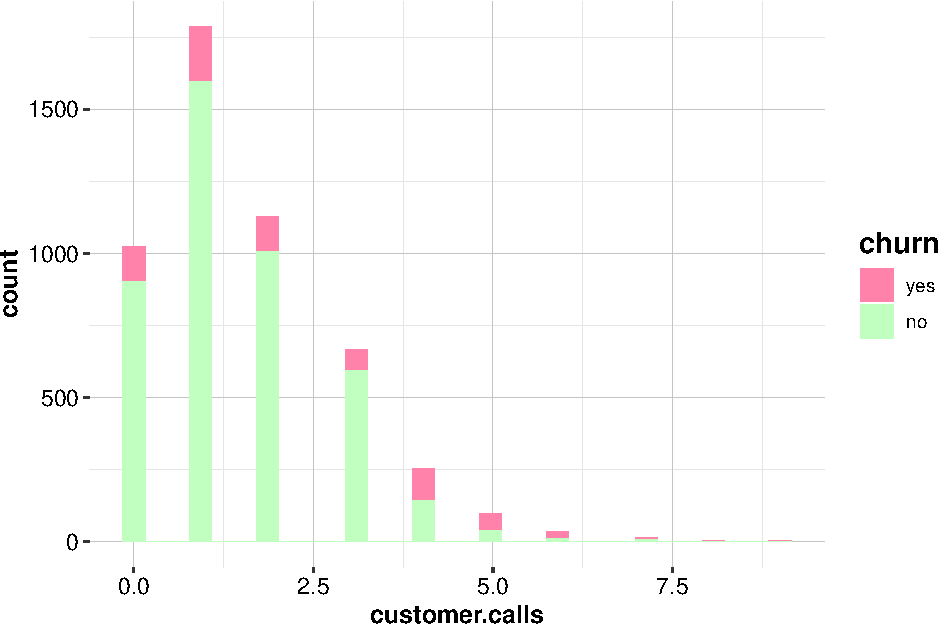
\includegraphics[width=0.5\linewidth]{EDA_files/figure-latex/unnamed-chunk-10-1} 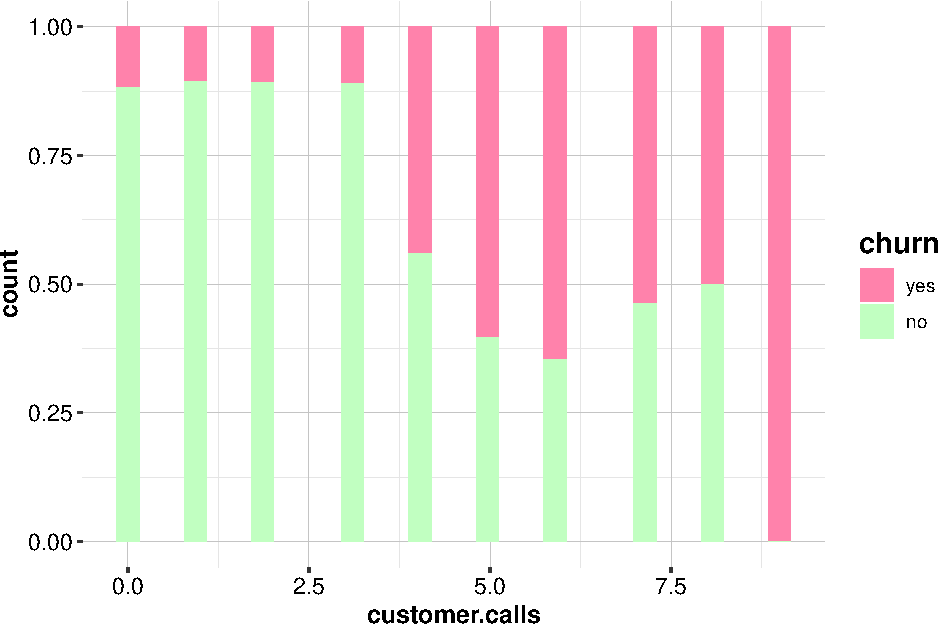
\includegraphics[width=0.5\linewidth]{EDA_files/figure-latex/unnamed-chunk-10-2}

The normalized histogram (right) reveals a striking trend: customers making \emph{four or more} service calls have a significantly higher churn rate. This suggests that frequent service interactions may indicate unresolved issues, leading to customer dissatisfaction.

Key Insights and Business Implications:

\begin{itemize}
\tightlist
\item
  Customers making frequent service calls are at higher risk of churning.\\
\item
  Companies could implement proactive retention strategies when a customer makes multiple calls, such as escalating issues or offering incentives after the third call.\\
\item
  This variable is likely to be a strong predictor in churn models and should be included in further analysis.
\end{itemize}

\subsection*{Daytime Minutes and Churn}\label{daytime-minutes-and-churn}
\addcontentsline{toc}{subsection}{Daytime Minutes and Churn}

Next, we examine \passthrough{\lstinline!day.mins!}, which represents the number of minutes a customer spends on daytime calls. We use box plots and density plots to compare distributions between churners and non-churners.

\begin{lstlisting}[language=R]
ggplot(data = churn) +
    geom_boxplot(aes(x = churn, y = day.mins), 
                 fill = c("palevioletred1", "darkseagreen1"))

ggplot(data = churn) +
    geom_density(aes(x = day.mins, fill = churn), alpha = 0.3)
\end{lstlisting}

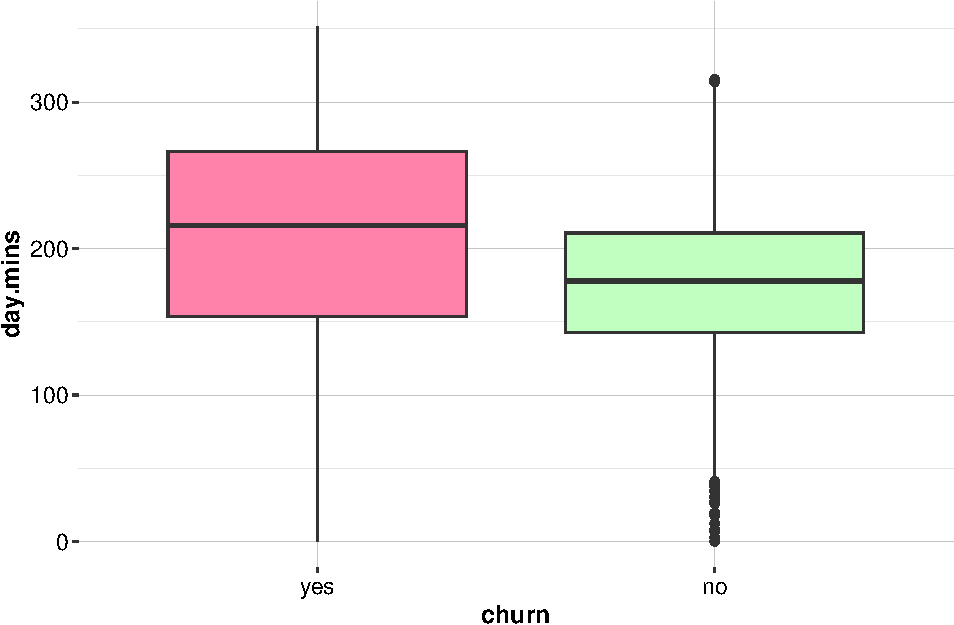
\includegraphics[width=0.5\linewidth]{EDA_files/figure-latex/unnamed-chunk-11-1} 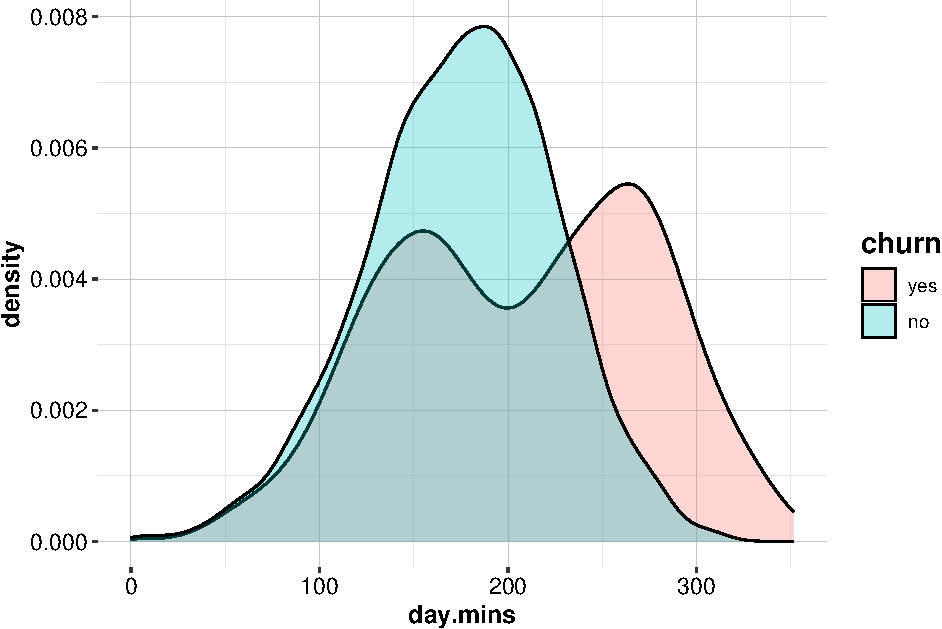
\includegraphics[width=0.5\linewidth]{EDA_files/figure-latex/unnamed-chunk-11-2}

The box plot (left) shows that customers who churn tend to have higher daytime call usage. The density plot (right) confirms this, with a noticeable peak in churners at higher \passthrough{\lstinline!day.mins!} values.

Key Insights and Business Implications:

\begin{itemize}
\tightlist
\item
  High \passthrough{\lstinline!day.mins!} usage is associated with increased churn.\\
\item
  Customers with extensive daytime usage may be dissatisfied with pricing or service quality.\\
\item
  Targeted retention offers, such as flexible rate plans for heavy users, could help mitigate churn.
\end{itemize}

\subsection*{Evening and Nighttime Minutes}\label{evening-and-nighttime-minutes}
\addcontentsline{toc}{subsection}{Evening and Nighttime Minutes}

To investigate whether evening and nighttime call patterns also relate to churn, we plot \passthrough{\lstinline!eve.mins!} and \passthrough{\lstinline!night.mins!}.

\begin{lstlisting}[language=R]
ggplot(data = churn) +
    geom_boxplot(aes(x = churn, y = eve.mins), fill = c("palevioletred1", "darkseagreen1"))

ggplot(data = churn) +
    geom_density(aes(x = eve.mins, fill = churn), alpha = 0.3)
\end{lstlisting}

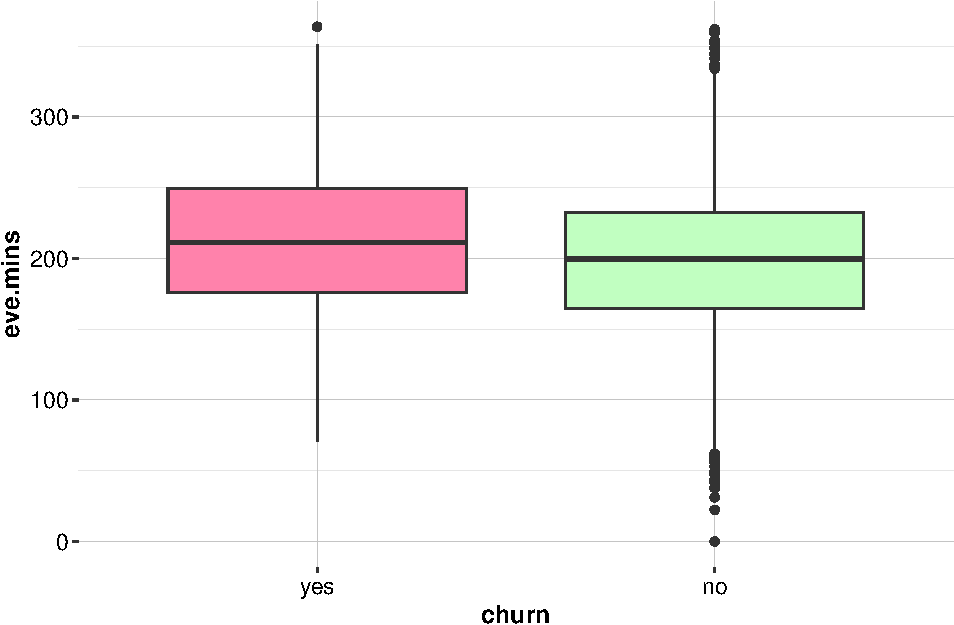
\includegraphics[width=0.5\linewidth]{EDA_files/figure-latex/unnamed-chunk-12-1} 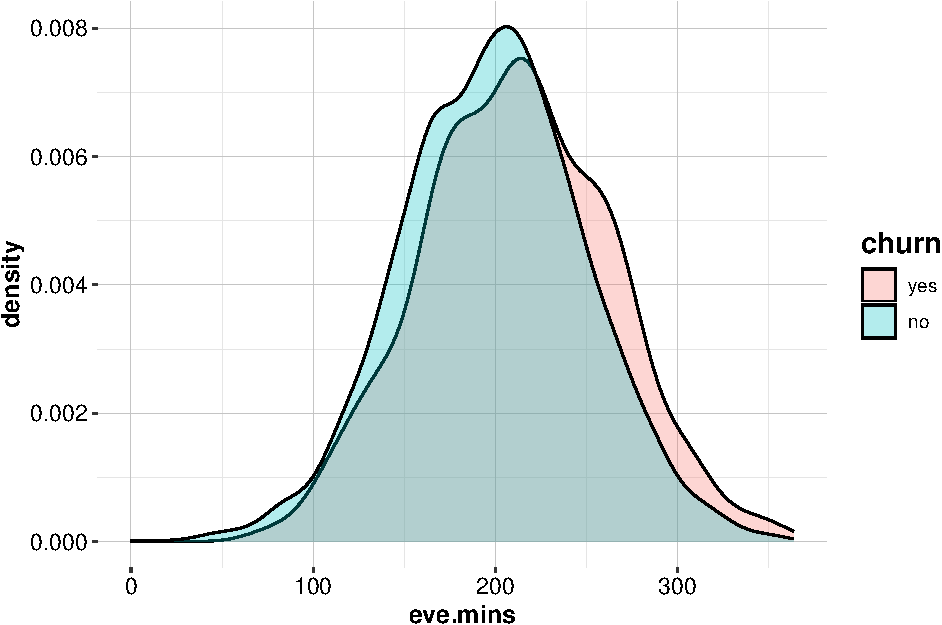
\includegraphics[width=0.5\linewidth]{EDA_files/figure-latex/unnamed-chunk-12-2}

While a slight trend suggests that churners have higher \passthrough{\lstinline!eve.mins!}, the effect is weaker than for \passthrough{\lstinline!day.mins!}. Similarly, analysis of \passthrough{\lstinline!night.mins!} does not reveal a clear distinction between churners and non-churners.

\begin{lstlisting}[language=R]
ggplot(data = churn) +
    geom_boxplot(aes(x = churn, y = night.mins), fill = c("palevioletred1", "darkseagreen1"))

ggplot(data = churn) +
    geom_density(aes(x = night.mins, fill = churn), alpha = 0.3)
\end{lstlisting}

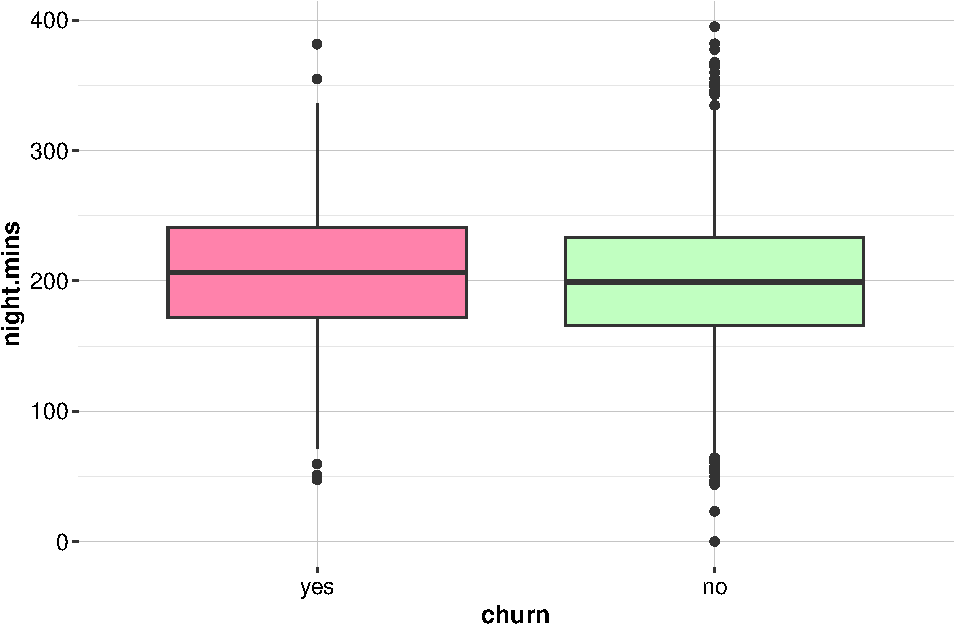
\includegraphics[width=0.5\linewidth]{EDA_files/figure-latex/unnamed-chunk-13-1} 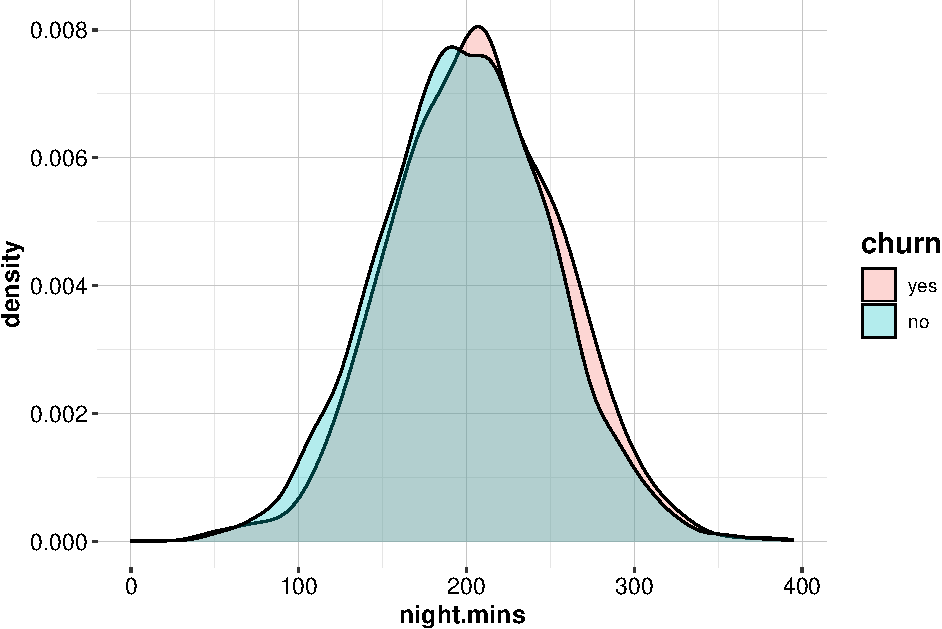
\includegraphics[width=0.5\linewidth]{EDA_files/figure-latex/unnamed-chunk-13-2}

The similar distributions suggest that nighttime call usage is not a strong churn indicator.

Key Insights and Business Implications:

\begin{itemize}
\tightlist
\item
  Unlike daytime calls, evening and nighttime minutes do not strongly predict churn.\\
\item
  Focusing on daytime usage and service call patterns may yield better predictive power.\\
\item
  Further statistical testing (e.g., t-tests or logistic regression) could confirm whether subtle differences exist.
\end{itemize}

Your subsection is \textbf{well-structured} and provides a \textbf{clear} overview of the analysis. However, there are a few \textbf{areas for improvement} in terms of \textbf{clarity, conciseness, and flow}. Below is an improved version that maintains the \textbf{same structure and meaning} while enhancing \textbf{readability and coherence}.

\subsection*{International Calls and Churn}\label{international-calls-and-churn}
\addcontentsline{toc}{subsection}{International Calls and Churn}

We now examine \passthrough{\lstinline!intl.calls!}, which represents the total number of international calls made by customers. To explore its relationship with churn, we visualize the distribution using box plots and density plots.

\begin{lstlisting}[language=R]
ggplot(data = churn) +
    geom_boxplot(aes(x = churn, y = intl.calls), 
                 fill = c("palevioletred1", "darkseagreen1"))

ggplot(data = churn) +
    geom_density(aes(x = intl.calls, fill = churn), alpha = 0.3)
\end{lstlisting}

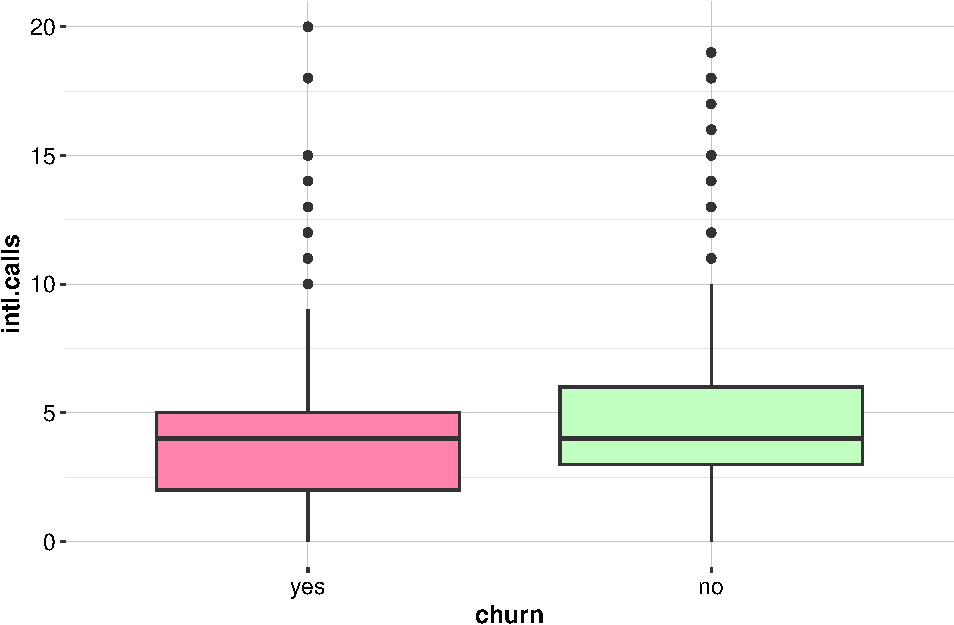
\includegraphics[width=0.5\linewidth]{EDA_files/figure-latex/unnamed-chunk-14-1} 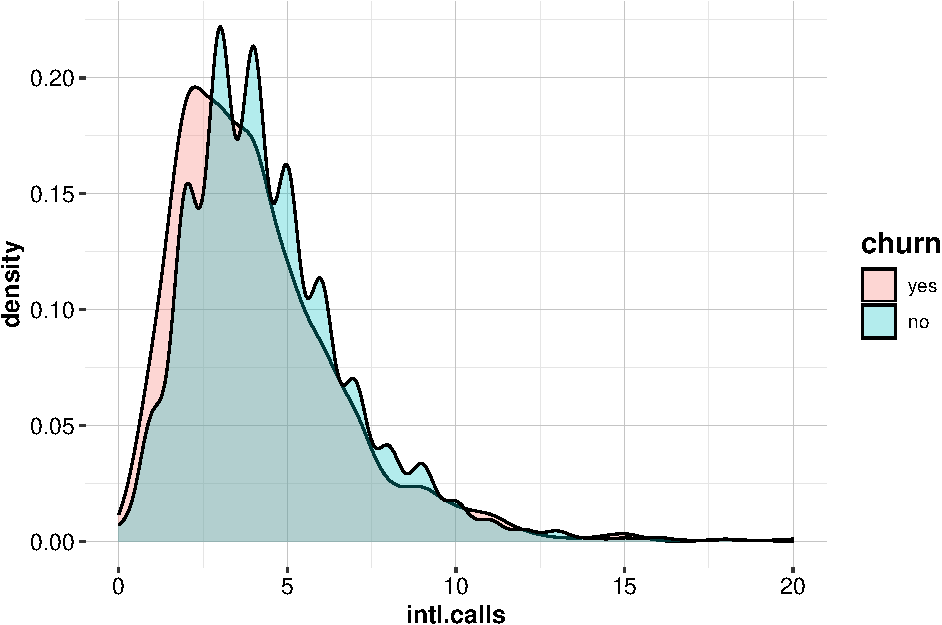
\includegraphics[width=0.5\linewidth]{EDA_files/figure-latex/unnamed-chunk-14-2}

The box plot (left) indicates that churners (\passthrough{\lstinline!churn=yes!}) tend to make slightly fewer international calls than non-churners. The density plot (right) further supports this, showing a minor difference in distribution between the two groups.

Although there is a slight trend suggesting that churners make fewer international calls on average, the difference does not appear substantial. This suggests that \passthrough{\lstinline!intl.calls!} is not a strong predictor of churn. To confirm whether this relationship is statistically significant, further testing---such as a two-sample t-test or logistic regression---would be required. In Section \ref{two-sample-t-test} of the next chapter, we demonstrate how to formally test this relationship using statistical methods.

\subsubsection*{Final Takeaways}\label{final-takeaways}
\addcontentsline{toc}{subsubsection}{Final Takeaways}

\begin{itemize}
\tightlist
\item
  \passthrough{\lstinline!customer.calls!} and \passthrough{\lstinline!day.mins!} are \emph{strongly associated} with churn and should be key predictors in churn models.\\
\item
  \emph{Customers making four or more service calls} are at high risk of leaving.\\
\item
  \emph{High daytime minute usage} is another important churn indicator, possibly due to pricing concerns.\\
\item
  Evening and nighttime call usage shows \emph{no strong relationship} with churn, suggesting it may not be an essential predictive feature.
\end{itemize}

By focusing on service calls and daytime minutes, companies can take targeted action to reduce churn, such as optimizing customer support escalation processes and offering personalized rate plans. These findings also guide the feature selection process for future predictive modeling efforts.

\section{Investigating Multivariate Relationships}\label{EDA-sec-multivariate}

While univariate analysis provides insights into individual variables, multivariate analysis helps uncover interactions that may influence churn. Examining variable relationships can reveal behavioral patterns that might not be evident when analyzing each feature in isolation.

A useful example is the relationship between \passthrough{\lstinline!day.mins!} (Day Minutes) and \passthrough{\lstinline!eve.mins!} (Evening Minutes), visualized in the scatter plot below:

\begin{lstlisting}[language=R]
ggplot(data = churn) +
    geom_point(aes(x = eve.mins, y = day.mins, color = churn), size = 0.7, alpha = 0.8) +
    scale_color_manual(values = c("palevioletred1", "darkseagreen1")) +
    geom_abline(intercept = 400, slope = -0.6, color = "blue", size = 1)
\end{lstlisting}

\begin{center}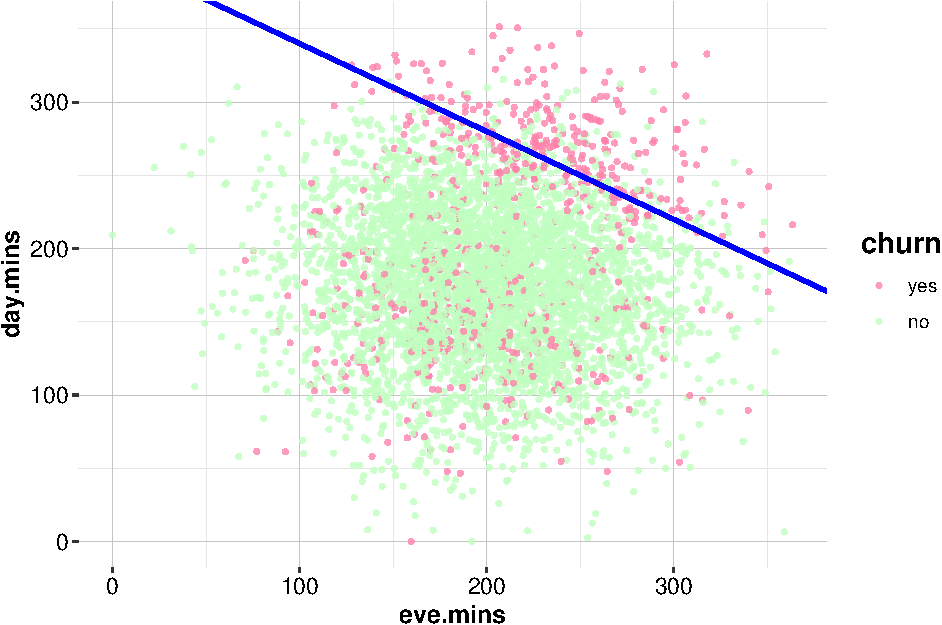
\includegraphics[width=0.7\linewidth]{EDA_files/figure-latex/unnamed-chunk-15-1} \end{center}

The diagonal line, represented by the equation:

\[
\text{day.mins} = 400 - 0.6 \times \text{eve.mins}
\]

separates the dataset into two regions. Customers in the upper-right region, where both day and evening minutes are high, exhibit a noticeably higher churn rate. This pattern was not apparent in the univariate analysis of \passthrough{\lstinline!eve.mins!}, demonstrating how feature interactions can provide deeper insights.

To quantify this effect, we isolate the high-churn segment:

\begin{lstlisting}[language=R]
sub_churn = subset(churn, (day.mins > 400 - 0.6 * eve.mins))

ggplot(data = sub_churn, aes(x = churn, label = scales::percent(prop.table(stat(count))))) +
    geom_bar(fill = c("palevioletred1", "darkseagreen1")) + 
    geom_text(stat = 'count', vjust = 0.2, size = 6)
\end{lstlisting}

\begin{center}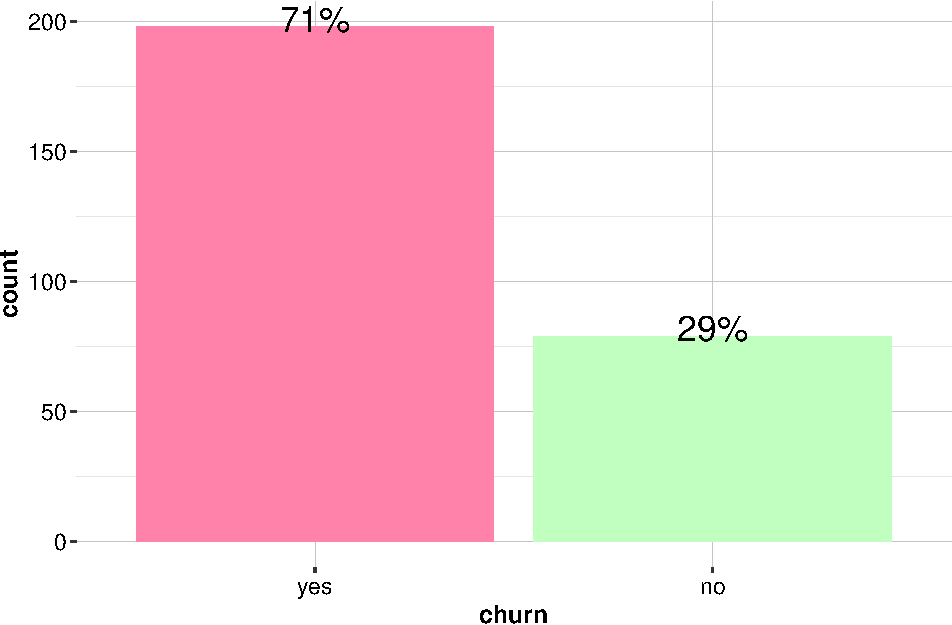
\includegraphics[width=0.7\linewidth]{EDA_files/figure-latex/unnamed-chunk-16-1} \end{center}

Within this subset, the churn rate is significantly higher than in the overall dataset, reinforcing the importance of considering variable interactions. The combination of high day and evening usage may indicate a specific customer behavior pattern that correlates with dissatisfaction.

Another key relationship exists between \passthrough{\lstinline!customer.calls!} and \passthrough{\lstinline!day.mins!}:

\begin{lstlisting}[language=R]
ggplot(data = churn) +
  geom_point(aes(x = day.mins, y = customer.calls, color = churn), alpha = 0.8) +
  scale_color_manual(values = c("palevioletred1", "darkseagreen1"))
\end{lstlisting}

\begin{center}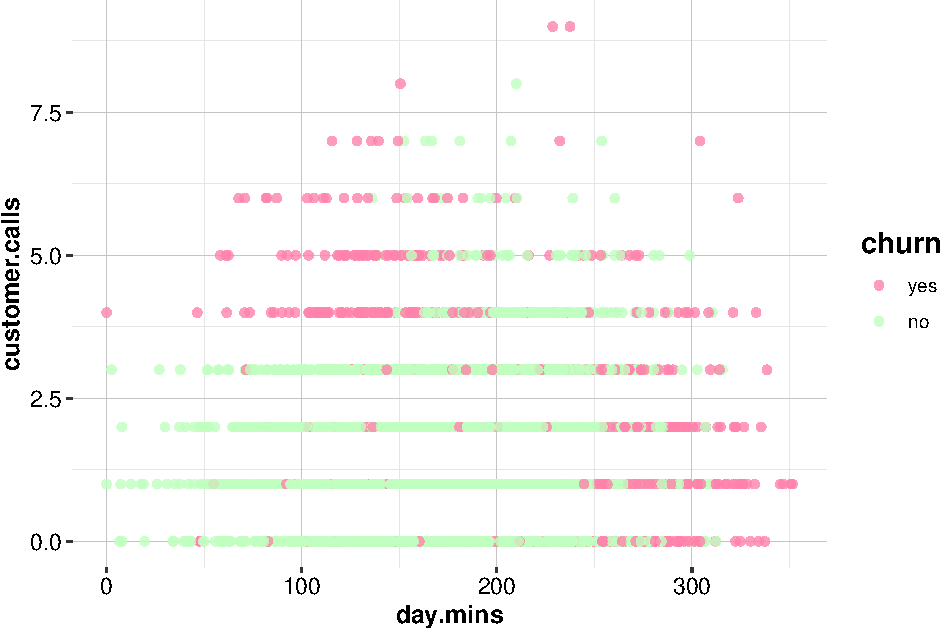
\includegraphics[width=0.7\linewidth]{EDA_files/figure-latex/unnamed-chunk-17-1} \end{center}

This scatter plot reveals an interesting high-churn region in the upper left, where customers make frequent customer service calls but have low day-minute usage. This group may represent dissatisfied customers who are not heavy users but are still experiencing service-related frustrations. By contrast, high-minute users who also make frequent service calls show a lower churn rate, possibly indicating that engaged customers are more tolerant of service issues.

\subsubsection*{Key Takeaways}\label{key-takeaways}
\addcontentsline{toc}{subsubsection}{Key Takeaways}

\begin{itemize}
\tightlist
\item
  Multivariate analysis reveals that customers with both high day and evening call usage have a much higher churn rate.
\item
  Customers making frequent customer service calls but using few daytime minutes are also at a higher risk of leaving.
\item
  The interaction between frequent customer service calls and high call usage suggests that dissatisfaction alone does not always drive churn---usage patterns also play a role.
\item
  Identifying customers in high-churn regions of these scatter plots can help in targeted retention efforts.
\end{itemize}

In Chapter \ref{chapter-statistics}, we will move from exploratory insights to formal statistical analysis, applying techniques to quantify these relationships and assess their predictive value.

\subsection{Investigating Correlated Variables}\label{investigating-correlated-variables}

Correlation measures the degree to which two variables move together. A positive correlation means that as one variable increases, the other also increases. A negative correlation indicates that when one variable rises, the other decreases. If two variables have no correlation, changes in one provide no information about changes in the other.

A common misconception is that correlation implies causation. For example, if an analysis finds that customers who make more calls to customer service tend to have higher churn rates, it does not necessarily mean that calling customer service causes churn. It could be that dissatisfied customers are more likely to call for assistance before leaving, making the number of service calls a symptom rather than a cause.

The strength and direction of a correlation are measured by the correlation coefficient, denoted as \(r\), which ranges from -1 to 1. A value of 1 indicates a perfect positive relationship, while -1 represents a perfect negative correlation. A value near zero suggests no linear relationship. In large datasets, even small correlations may be statistically significant, but practical significance must also be considered. A correlation of 0.05 might be significant in a dataset with thousands of observations, but it is unlikely to provide meaningful predictive power.

Below, Figure \ref{fig:correlation} shows examples of different correlation coefficients.

\begin{figure}

{\centering \includegraphics[width=1\linewidth]{images/correlation} 

}

\caption{Example scatterplots showing different correlation coefficients.}\label{fig:correlation}
\end{figure}

When multiple variables are highly correlated, redundancy can become a problem. Including both variables in a model may not add much new information and can lead to instability, particularly in regression-based models where multicollinearity makes it difficult to determine the effect of individual predictors. Instead of automatically removing correlated variables, a more thoughtful approach involves assessing their practical relevance and whether they provide distinct information.

To examine correlations in the churn dataset, we compute the correlation matrix for the numerical variables and visualize it using a heatmap.

\begin{lstlisting}[language=R]
library(ggcorrplot)  
variable_list = c("intl.mins",  "intl.calls",  "intl.charge", 
                  "day.mins",   "day.calls",   "day.charge",
                  "eve.mins",   "eve.calls",   "eve.charge",
                  "night.mins", "night.calls", "night.charge")

cor_matrix = cor(churn[, variable_list])

ggcorrplot(cor_matrix, type = "lower", lab = TRUE, lab_size = 3)
\end{lstlisting}

\begin{center}\includegraphics[width=1\linewidth]{EDA_files/figure-latex/unnamed-chunk-18-1} \end{center}

The correlation matrix highlights some key relationships. The charge variables are perfectly correlated with their corresponding minutes variables because charges are calculated directly from call duration. Including both would introduce redundancy. To avoid this, the charge variables should be removed, keeping only the minutes variables.

Another notable observation is that the number of calls within each time period is not strongly correlated with total minutes. One might expect that customers who make more calls would also spend more time on the phone, but the data does not support this assumption. This suggests that call frequency and call duration may capture different aspects of customer behavior, making it valuable to retain both types of variables for modeling.

By addressing correlations during exploratory data analysis, the dataset can be refined to ensure that only the most informative variables are used in predictive modeling. Removing redundant features reduces complexity while retaining meaningful signals, improving the interpretability and performance of models.

\section{Key Findings and Insights}\label{key-findings-and-insights}

The exploratory data analysis of the churn dataset has provided a deeper understanding of the factors influencing customer attrition. By examining individual variables and their interactions, we identified several key trends that will inform predictive modeling and business strategy.

One of the most striking findings is the role of customer service interactions in churn. Customers who have made four or more calls to customer service are significantly more likely to leave. This suggests that frequent interactions may indicate unresolved complaints, leading to dissatisfaction. Additionally, customers with both high daytime and evening call usage exhibit churn rates up to six times higher than average, indicating that high usage may correlate with dissatisfaction---perhaps due to service quality concerns or pricing issues.

The international calling plan also appears to be a strong predictor of churn. Customers who subscribe to this plan are leaving at a much higher rate, suggesting that the plan may not be delivering sufficient value. In contrast, customers with a voice mail plan show a lower churn rate, indicating that this feature may contribute to customer retention.

Several variables, while not directly linked to churn in univariate analysis, could still provide value when combined with other features in predictive modeling. For example, customers with relatively low daytime usage but frequent customer service calls show a higher likelihood of leaving, a pattern that suggests service dissatisfaction among lower-usage customers.

From a modeling perspective, some variables introduce redundancy. The charge variables (day, evening, night, and international) are perfectly correlated with their corresponding minute variables, as they are derived directly from them. Retaining only the minute variables will avoid multicollinearity while preserving all relevant information. Similarly, the area code and state fields may not contribute much to predictive power, as they do not show strong relationships with churn in this dataset.

\subsection*{Strategic Recommendations}\label{strategic-recommendations}
\addcontentsline{toc}{subsection}{Strategic Recommendations}

These findings present opportunities for targeted interventions to improve customer retention. Given that frequent customer service calls are a strong indicator of churn, companies should implement proactive escalation strategies. Customers making their third service call should receive priority attention, potentially with issue resolution specialists or targeted retention offers.

For high-usage customers, personalized plans and loyalty incentives could help reduce churn. Offering flexible pricing or additional benefits for high daytime and evening callers may address concerns that drive them to switch providers. Similarly, a review of the international plan is necessary to assess whether its pricing, service quality, or features are leading to dissatisfaction.

While some variables, such as night minutes and certain demographic features, do not show strong direct correlations with churn, they may still contribute when combined with other predictors in a machine learning model. Further analysis will determine their importance in a predictive framework.

By identifying these churn-related patterns early, businesses can take proactive steps to improve customer satisfaction and reduce attrition, strengthening overall retention efforts before relying on predictive modeling. These insights will serve as a foundation for the next stage of analysis, where machine learning models will be applied to quantify these relationships more precisely.

\section{Exercises}\label{exercises-2}

\subsection*{Conceptual Questions}\label{conceptual-questions}
\addcontentsline{toc}{subsection}{Conceptual Questions}

\begin{enumerate}
\def\labelenumi{\arabic{enumi}.}
\item
  Why is it important to perform exploratory data analysis before proceeding to the modeling phase? What are the potential risks of skipping EDA and directly applying data mining techniques?
\item
  If a predictor does not exhibit a clear relationship with the target variable during exploratory data analysis, should it be omitted from the modeling stage? Justify your answer by considering potential interactions, hidden patterns, and the role of feature selection.
\item
  What does it mean for two variables to be correlated? Explain the concept of correlation, including its direction and strength, and discuss how it differs from causation. Provide an example to illustrate your explanation.
\item
  How can you identify and address correlated variables during exploratory data analysis? Describe the steps you would take to manage correlated predictors effectively and explain the benefits of this approach for predictive modeling.
\item
  What are the consequences of including highly correlated variables in a predictive model? Discuss the impact of multicollinearity on model performance, interpretability, and stability, and explain how it can be detected and addressed.
\item
  Is it always advisable to remove one of two correlated predictors from a model? Discuss the advantages and drawbacks of this approach, and explain under what circumstances keeping both predictors might be beneficial.
\item
  For each of the following descriptive methods, determine whether it applies to categorical data, continuous numerical data, or both. Provide a brief explanation of how each method is used in exploratory data analysis.

  \begin{itemize}
  \tightlist
  \item
    Histograms\\
  \item
    Box plots\\
  \item
    Density plots\\
  \item
    Scatter plots\\
  \item
    Summary statistics\\
  \item
    Correlation analysis\\
  \item
    Contingency tables\\
  \item
    Bar plots\\
  \item
    Heatmaps
  \end{itemize}
\item
  A telecommunications company is analyzing customer data to identify factors influencing churn. During exploratory data analysis, they discover that customers with both high day minutes and high evening minutes have a significantly higher churn rate. What actionable insights could the company derive from this finding, and how might they use this information to reduce customer attrition?
\item
  Suppose you are conducting exploratory data analysis on a dataset with 20 predictor variables. After examining the correlation matrix, you find that several pairs of variables are highly correlated (r \textgreater{} 0.9). How would you address these correlations to ensure the reliability and interpretability of your predictive models? Describe the steps you would take to manage these correlated variables effectively.
\item
  Discuss the importance of considering both statistical and practical implications when evaluating correlations during exploratory data analysis. Provide an example of a statistically significant correlation that may not have real-world significance, and explain why it is essential to consider both aspects in data analysis.
\item
  Why is it important to investigate multivariate relationships rather than relying only on univariate analysis? Provide an example where an interaction between two variables reveals a pattern that would be missed in separate univariate analyses.
\item
  How does data visualization aid in the exploratory data analysis process? Discuss at least two specific examples where visualizations provide insights that summary statistics alone cannot reveal.
\item
  Suppose you discover that customers who have high daytime call usage and make frequent customer service calls are more likely to churn. What business actions could be taken based on this insight?
\item
  Outliers can be influential in statistical modeling. What are some possible causes of outliers in a dataset? How would you decide whether to keep, modify, or remove an outlier?
\item
  In the context of exploratory data analysis, explain why missing values are a critical issue. What are the different strategies for handling missing values, and under what circumstances would each be appropriate?
\end{enumerate}

\subsection*{Hands-On Practice: Exploring the Bank Dataset}\label{hands-on-practice-exploring-the-bank-dataset}
\addcontentsline{toc}{subsection}{Hands-On Practice: Exploring the Bank Dataset}

For hands-on practice, we will explore the \emph{bank} dataset available in the \textbf{R} package \textbf{liver}. The \emph{bank} dataset is related to direct marketing campaigns of a Portuguese banking institution. The campaigns were conducted via phone calls, with multiple contacts sometimes needed to determine whether a client would subscribe to a term deposit. The goal of this dataset is to predict whether a client will subscribe to a term deposit, which will be explored using classification techniques in Chapters \ref{chapter-knn} and \ref{chapter-nn}.

More details on this dataset can be found at: \url{https://rdrr.io/cran/liver/man/bank.html}.

We can import the dataset in \textbf{R} as follows:

\begin{lstlisting}[language=R]
library(liver)
data(bank)      
\end{lstlisting}

To examine the dataset's structure, we use:

\begin{lstlisting}[language=R]
str(bank)
   'data.frame':    4521 obs. of  17 variables:
    $ age      : int  30 33 35 30 59 35 36 39 41 43 ...
    $ job      : Factor w/ 12 levels "admin.","blue-collar",..: 11 8 5 5 2 5 7 10 3 8 ...
    $ marital  : Factor w/ 3 levels "divorced","married",..: 2 2 3 2 2 3 2 2 2 2 ...
    $ education: Factor w/ 4 levels "primary","secondary",..: 1 2 3 3 2 3 3 2 3 1 ...
    $ default  : Factor w/ 2 levels "no","yes": 1 1 1 1 1 1 1 1 1 1 ...
    $ balance  : int  1787 4789 1350 1476 0 747 307 147 221 -88 ...
    $ housing  : Factor w/ 2 levels "no","yes": 1 2 2 2 2 1 2 2 2 2 ...
    $ loan     : Factor w/ 2 levels "no","yes": 1 2 1 2 1 1 1 1 1 2 ...
    $ contact  : Factor w/ 3 levels "cellular","telephone",..: 1 1 1 3 3 1 1 1 3 1 ...
    $ day      : int  19 11 16 3 5 23 14 6 14 17 ...
    $ month    : Factor w/ 12 levels "apr","aug","dec",..: 11 9 1 7 9 4 9 9 9 1 ...
    $ duration : int  79 220 185 199 226 141 341 151 57 313 ...
    $ campaign : int  1 1 1 4 1 2 1 2 2 1 ...
    $ pdays    : int  -1 339 330 -1 -1 176 330 -1 -1 147 ...
    $ previous : int  0 4 1 0 0 3 2 0 0 2 ...
    $ poutcome : Factor w/ 4 levels "failure","other",..: 4 1 1 4 4 1 2 4 4 1 ...
    $ deposit  : Factor w/ 2 levels "no","yes": 1 1 1 1 1 1 1 1 1 1 ...
\end{lstlisting}

\begin{enumerate}
\def\labelenumi{\arabic{enumi}.}
\setcounter{enumi}{15}
\item
  \emph{Dataset Overview}: Report the summary statistics of the dataset, including the types of variables. What can you infer from the structure of the data?
\item
  \emph{Target Variable Analysis}: Generate a bar plot for the target variable \passthrough{\lstinline!deposit!} using the \passthrough{\lstinline!ggplot()!} function from \textbf{ggplot2}. What is the proportion of clients who subscribed to a term deposit?
\item
  \emph{Binary Variable Exploration}: Investigate the binary categorical variables \passthrough{\lstinline!default!}, \passthrough{\lstinline!housing!}, and \passthrough{\lstinline!loan!}. Create contingency tables and bar plots to visualize their distributions. What insights can you draw from these variables?
\item
  \emph{Exploring Numerical Variables}: Analyze the numerical variables in the dataset. Create histograms and box plots to visualize their distributions. Identify any patterns, skewness, or unusual observations.
\item
  \emph{Outlier Detection}: Identify whether any numerical variables contain outliers. How would you handle these outliers to maintain data integrity while ensuring robust analysis?
\item
  \emph{Correlation Analysis}: Compute the correlation matrix for the numerical variables. Identify pairs of highly correlated variables. What strategies would you use to handle these correlations to avoid redundancy and multicollinearity in predictive modeling?
\item
  \emph{Key EDA Findings}: Summarize the key findings from your exploratory data analysis based on the exercises above. If you were preparing a formal report, how would you highlight notable patterns, relationships, or anomalies?
\item
  \emph{Business Implications}: Based on your findings, what actionable insights could the bank derive from this exploratory analysis? How could these insights help in optimizing marketing strategies and improving customer targeting?
\item
  \emph{Multivariate Analysis}: Investigate the relationship between the number of previous marketing campaign contacts (\passthrough{\lstinline!campaign!}) and term deposit subscriptions (\passthrough{\lstinline!deposit!}). Does higher contact frequency correlate with increased subscriptions? Use a box plot or bar chart to support your findings.
\item
  \emph{Feature Engineering Insight}: Based on your EDA, propose at least one new feature that could improve the predictive power of a classification model for term deposit subscriptions. Justify your reasoning.
\item
  \emph{Seasonality Effects}: Investigate whether the time of year influences term deposit subscriptions by analyzing the \passthrough{\lstinline!month!} variable. Do certain months have a higher success rate? Visualize this pattern and discuss its potential business implications.
\item
  \emph{Effect of Employment Type}: Examine how the \passthrough{\lstinline!job!} variable relates to term deposit subscriptions. Which job categories have higher success rates? Present your findings using a suitable visualization and discuss how banks could use this insight for targeted marketing.
\item
  \emph{Interaction Effects}: Analyze whether interactions between different predictors, such as \passthrough{\lstinline!education!} and \passthrough{\lstinline!job!}, influence the likelihood of subscribing to a term deposit. Use appropriate visualizations or statistical summaries to support your findings.
\item
  \emph{Effect of Contact Duration}: Investigate whether the duration of the last contact (\passthrough{\lstinline!duration!} variable) has a strong relationship with term deposit subscription. Visualize the distribution and discuss whether longer calls are associated with higher success rates.
\item
  \emph{Comparison of Campaign Outcomes}: Compare the subscription rates (\passthrough{\lstinline!deposit!} variable) across different types of marketing campaigns (\passthrough{\lstinline!campaign!} variable). What trends emerge, and how could they inform future marketing strategies?
\end{enumerate}

\chapter{Statistical Inference and Hypothesis Testing}\label{chapter-statistics}

Statistical inference bridges the gap between \emph{what we observe in a sample} and \emph{what we want to understand about the population}. While exploratory data analysis (EDA) helps us identify patterns and relationships, statistical inference allows us to determine whether these patterns hold beyond our sample---or whether they could have arisen by chance. In this chapter, we transition from \emph{exploring} data to \emph{validating} insights through estimation, hypothesis testing, and quantifying uncertainty.

The goals of statistical inference can be summarized into three fundamental tasks:

\begin{enumerate}
\def\labelenumi{\arabic{enumi}.}
\tightlist
\item
  \emph{Estimating population characteristics}, such as averages or proportions, based on sample data.\\
\item
  \emph{Quantifying uncertainty} to measure how confident we can be in our results.\\
\item
  \emph{Testing hypotheses} to evaluate whether observed patterns are statistically meaningful or simply due to random variation.
\end{enumerate}

These tasks form the foundation of \emph{data-driven decision-making}, enabling us to distinguish meaningful insights from statistical noise. In this chapter, we will explore these three pillars---estimation, uncertainty, and hypothesis testing---using intuitive explanations and practical examples.

But statistical inference isn't just about applying formulas---it's also about \emph{critical thinking}. By the end of this chapter, you'll develop two essential skills:

\begin{itemize}
\tightlist
\item
  \emph{How to detect statistical misuses and misleading claims}, helping you critically evaluate data-driven arguments.\\
\item
  \emph{How to avoid common pitfalls in statistical analysis}, ensuring that your own conclusions are both sound and defensible.
\end{itemize}

For those interested in the art of identifying statistical manipulation, Darrell Huff's classic book, \href{https://www.goodreads.com/book/show/51291.How_to_Lie_with_Statistics}{\emph{How to Lie with Statistics}}, offers timeless lessons in statistical skepticism. Understanding these techniques is valuable not just for avoiding errors but also for recognizing when data is being used to mislead.

Let's dive in and learn how to make statistical inferences with confidence, curiosity, and a healthy dose of skepticism.

\section{Estimation: Using Data to Make Predictions}\label{estimation-using-data-to-make-predictions}

Estimation is a fundamental aspect of statistical inference that allows us to make informed guesses about a population based on a sample. Rather than relying on the entire population, which is often impractical, we use sample data to estimate key characteristics such as averages or proportions. For instance, in the churn dataset, we might want to estimate:

\begin{itemize}
\tightlist
\item
  The \emph{average number of customer service calls} among churners.\\
\item
  The \emph{proportion of customers} subscribed to the International Plan.
\end{itemize}

There are two main types of estimation:

\begin{enumerate}
\def\labelenumi{\arabic{enumi}.}
\tightlist
\item
  \emph{Point estimation} provides a single best guess for a population parameter, such as using the sample mean to estimate the population mean.\\
\item
  \emph{Interval estimation} gives a range of plausible values (a confidence interval) within which the true population parameter is likely to fall.
\end{enumerate}

Let's explore some examples:

\begin{example}
\protect\hypertarget{exm:ex-est-churn-proportion}{}\label{exm:ex-est-churn-proportion}To estimate the \emph{proportion of churners} in the dataset, we use the \emph{sample proportion} as a point estimate for the population proportion. Here's how to calculate it in R:

\begin{lstlisting}[language=R]
library(liver)
data(churn) 

prop.table(table(churn$churn))["yes"]
      yes 
   0.1414
\end{lstlisting}

The estimated proportion of churners in the dataset is 0.14, serving as our best guess for the proportion of churners in the population.
\end{example}

\begin{example}
\protect\hypertarget{exm:ex-est-service-call}{}\label{exm:ex-est-service-call}Now, let's estimate the \emph{average number of customer service calls} for customers who churned. The \emph{sample mean} serves as a point estimate for the population mean:

\begin{lstlisting}[language=R]
# Filter churners
churned_customers <- churn[churn$churn == "yes", ]

# Calculate the mean
mean_calls <- mean(churned_customers$customer.calls)
cat("Point Estimate: Average Customer Service Calls for Churners:", mean_calls)
   Point Estimate: Average Customer Service Calls for Churners: 2.254597
\end{lstlisting}

If the sample mean is \textbf{4 calls}, this would be our best estimate of the average number of customer service calls among all churners in the population.
\end{example}

\begin{quote}
\emph{While point estimates are useful, they provide no information about uncertainty. Confidence intervals help quantify the precision of an estimate, which we explore next.}
\end{quote}

\section{Quantifying Uncertainty: Confidence Intervals}\label{statistics-confidence-interval}

Confidence intervals help quantify uncertainty when estimating population parameters. Instead of simply stating that ``the average number of customer service calls is 4,'' a confidence interval provides a range, such as ``we are 95\% confident that the true average is between 3.8 and 4.2.'' This range accounts for sampling variability, offering a clearer picture of how reliable the estimate is.

A confidence interval consists of a point estimate, such as a sample mean or proportion, and a margin of error, which accounts for uncertainty. The general form of a confidence interval is:

\[
\text{Point Estimate}  \pm \text{Margin of Error}
\]

For a population mean, the confidence interval is calculated as:

\[
\bar{x} \pm z_{\frac{\alpha}{2}} \times \left( \frac{s}{\sqrt{n}} \right),
\]

where \(\bar{x}\) is the sample mean, \(z_{\frac{\alpha}{2}}\) is a critical value from the standard normal distribution (such as 1.96 for a 95\% confidence level), \(s\) is the sample standard deviation, and \(n\) is the sample size. This concept is illustrated in Figure \ref{fig:confidence-interval}, where the interval is centered around the point estimate and its width depends on the margin of error.

\begin{figure}

{\centering \includegraphics[width=0.8\linewidth]{images/confidence_interval} 

}

\caption{Confidence interval for the population mean. The interval is centered around the point estimate, with the width determined by the margin of error. The confidence level specifies the probability that the interval contains the true population parameter.}\label{fig:confidence-interval}
\end{figure}

Several factors influence the width of a confidence interval. Larger sample sizes generally yield narrower intervals, increasing precision, while higher variability in the data results in wider intervals. The choice of confidence level also affects the width; for example, a 99\% confidence level produces a wider interval than a 90\% confidence level because it must capture more possible values.

Imagine you want to estimate the average height of all students in a university. If you survey only 10 students, your confidence interval will be wide because you have little data. But if you survey 1,000 students, your estimate becomes much more precise, and the confidence interval shrinks. This illustrates why larger sample sizes lead to more reliable estimates---more data reduces uncertainty and results in tighter confidence intervals.

To illustrate, suppose we want to estimate the average number of customer service calls among churners with 95\% confidence:

\begin{lstlisting}[language=R]
# Calculate mean and standard error
mean_calls <- mean(churned_customers$customer.calls)
se_calls <- sd(churned_customers$customer.calls) / sqrt(nrow(churned_customers))

# Confidence Interval
z_score <- 1.96  # For 95% confidence
ci_lower <- mean_calls - z_score * se_calls
ci_upper <- mean_calls + z_score * se_calls

cat("95% Confidence Interval: [", ci_lower, ",", ci_upper, "]")
   95% Confidence Interval: [ 2.120737 , 2.388457 ]
\end{lstlisting}

If the computed interval is {[}2.12, 2.39{]}, we can say with 95\% confidence that the true average number of service calls for churners falls within this range.

For smaller sample sizes, it is better to use the t-distribution instead of the normal distribution, as it accounts for the added uncertainty when estimating the population standard deviation. This adjustment is applied automatically in R when using the \passthrough{\lstinline!t.test()!} function:

\begin{lstlisting}[language=R]
t.test(churned_customers$customer.calls, conf.level = 0.95)$conf.int
   [1] 2.120509 2.388685
   attr(,"conf.level")
   [1] 0.95
\end{lstlisting}

Confidence intervals are particularly useful for comparing groups. If confidence intervals for two groups, such as churners and non-churners, do not overlap significantly, it suggests meaningful differences in behavior. By providing a range rather than a single estimate, confidence intervals help balance precision and uncertainty, making them a valuable tool in statistical inference.

\section{Hypothesis Testing}\label{hypothesis-testing}

Hypothesis testing provides a structured framework for evaluating claims about population parameters using sample data. It helps us assess whether patterns observed during exploratory analysis are statistically significant or simply the result of random variation. This method is fundamental to data-driven decision-making, enabling us to distinguish meaningful insights from noise.

At its core, hypothesis testing involves two competing statements about a population parameter:

\begin{itemize}
\tightlist
\item
  The \emph{null hypothesis} (\(H_0\)) represents the default assumption or status quo, often stating that there is no difference between groups, no effect of a treatment, or no relationship between variables.\\
\item
  The \emph{alternative hypothesis} (\(H_a\)) challenges \(H_0\), suggesting that a difference, effect, or relationship does exist.
\end{itemize}

Using sample evidence, we decide whether to:

\begin{itemize}
\tightlist
\item
  \emph{Reject \(H_0\)} and conclude that the data supports \(H_a\).\\
\item
  \emph{Fail to reject \(H_0\)}, meaning the evidence is insufficient to dismiss \(H_0\), though this does not prove it to be true.
\end{itemize}

The strength of the evidence against \(H_0\) is quantified using the \emph{p}-value, which represents the probability of obtaining the observed data---or something more extreme---if \(H_0\) were true. A smaller \emph{p}-value suggests stronger evidence against \(H_0\).

\begin{itemize}
\tightlist
\item
  If \(p < 0.05\), we reject \(H_0\) and conclude there is statistical evidence for \(H_a\).\\
\item
  If \(p > 0.05\), we fail to reject \(H_0\), meaning the evidence is not strong enough to support \(H_a\).
\end{itemize}

The threshold for decision-making is called the \emph{significance level} (\(\alpha\)), typically set at 0.05 (5\%). This value represents the maximum probability of making a \emph{Type I error}---incorrectly rejecting \(H_0\). In fields where errors have serious consequences, such as medicine or aerospace, stricter thresholds (e.g., \(\alpha = 0.01\)) are often used.

A simple takeaway, often emphasized in hypothesis testing, is:

Reject \(H_0\) if the \(p\)-value \textless{} \(\alpha\).

For example:\\
- If \(p = 0.03\) and \(\alpha = 0.05\), we reject \(H_0\) because \(p < \alpha\).\\
- If \(p = 0.12\), we fail to reject \(H_0\) because \(p > \alpha\).

Although \emph{p}-values provide a structured way to make decisions, they have limitations. A small \emph{p}-value does not necessarily mean a result is practically important---it only indicates statistical significance. Large datasets can generate small \emph{p}-values for trivial effects, while small datasets may fail to detect meaningful differences. Additionally, the binary reject/fail-to-reject approach can sometimes oversimplify interpretation.

\subsection{Types of Hypothesis Tests}\label{types-of-hypothesis-tests}

Depending on the research question, hypothesis tests can take different forms:

\begin{itemize}
\tightlist
\item
  \emph{Left-tailed test}: The alternative hypothesis states that the parameter is \emph{less than} a specified value (\(H_a: \theta < \theta_0\)). Example: Testing whether the average number of customer service calls is \emph{less than} 3.\\
\item
  \emph{Right-tailed test}: The alternative hypothesis states that the parameter is \emph{greater than} a specified value (\(H_a: \theta > \theta_0\)). Example: Testing whether the churn rate is \emph{greater than} 30\%.\\
\item
  \emph{Two-tailed test}: The alternative hypothesis states that the parameter is \emph{not equal to} a specified value (\(H_a: \theta \neq \theta_0\)), evaluating deviations in either direction. Example: Testing whether the mean monthly charges differ from \$50.
\end{itemize}

A useful analogy for hypothesis testing is a criminal trial. The \emph{null hypothesis} (\(H_0\)) represents the presumption of innocence, while the \emph{alternative hypothesis} (\(H_a\)) represents guilt. The jury weighs the evidence and either rejects \(H_0\) (convicts the defendant) or fails to reject \(H_0\) (acquits due to insufficient evidence). Just as juries can make errors, hypothesis tests also have two types of errors summarized in Table \ref{tab:hypothesis-errors}.

\begin{longtable}[]{@{}
  >{\raggedright\arraybackslash}p{(\linewidth - 4\tabcolsep) * \real{0.2680}}
  >{\raggedright\arraybackslash}p{(\linewidth - 4\tabcolsep) * \real{0.3711}}
  >{\raggedright\arraybackslash}p{(\linewidth - 4\tabcolsep) * \real{0.3608}}@{}}
\caption{\label{tab:hypothesis-errors} Possible outcomes of hypothesis testing with two correct decisions and two types of errors.}\tabularnewline
\toprule\noalign{}
\begin{minipage}[b]{\linewidth}\raggedright
\emph{Decision}
\end{minipage} & \begin{minipage}[b]{\linewidth}\raggedright
\emph{Reality: \(H_0\) is True}
\end{minipage} & \begin{minipage}[b]{\linewidth}\raggedright
\emph{Reality: \(H_0\) is False}
\end{minipage} \\
\midrule\noalign{}
\endfirsthead
\toprule\noalign{}
\begin{minipage}[b]{\linewidth}\raggedright
\emph{Decision}
\end{minipage} & \begin{minipage}[b]{\linewidth}\raggedright
\emph{Reality: \(H_0\) is True}
\end{minipage} & \begin{minipage}[b]{\linewidth}\raggedright
\emph{Reality: \(H_0\) is False}
\end{minipage} \\
\midrule\noalign{}
\endhead
\bottomrule\noalign{}
\endlastfoot
Fail to Reject \(H_0\) & {\emph{Correct Decision}: Acquit an innocent person.} & {\emph{Type II Error (\(\beta\))}: Acquit a guilty person.} \\
Reject \(H_0\) & {\emph{Type I Error (\(\alpha\))}: Convict an innocent person.} & {\emph{Correct Decision}: Convict a guilty person.} \\
\end{longtable}

A \emph{Type I Error} (\(\alpha\)) occurs when \(H_0\) is rejected even though it is true---similar to convicting an innocent person. A \emph{Type II Error} (\(\beta\)) happens when \(H_0\) is not rejected even though it is false---similar to acquitting a guilty person. The probability of a Type I error is controlled by the chosen significance level (\(\alpha\)), while the probability of a Type II error depends on factors like sample size and test sensitivity.

\subsection*{Common Hypothesis Tests}\label{common-hypothesis-tests}
\addcontentsline{toc}{subsection}{Common Hypothesis Tests}

There are several widely used hypothesis tests, as listed in Table \ref{tab:hypothesis-errors}, each suited to different types of data.

\begin{longtable}[]{@{}
  >{\raggedright\arraybackslash}p{(\linewidth - 4\tabcolsep) * \real{0.2437}}
  >{\raggedright\arraybackslash}p{(\linewidth - 4\tabcolsep) * \real{0.3277}}
  >{\raggedright\arraybackslash}p{(\linewidth - 4\tabcolsep) * \real{0.4286}}@{}}
\caption{\label{tab:hypothesis-test} Seven commonly used hypothesis tests, their null hypotheses (\(H_0\)), and the types of variables they apply to.}\tabularnewline
\toprule\noalign{}
\begin{minipage}[b]{\linewidth}\raggedright
Test
\end{minipage} & \begin{minipage}[b]{\linewidth}\raggedright
\(H_0\)
\end{minipage} & \begin{minipage}[b]{\linewidth}\raggedright
Can be used for
\end{minipage} \\
\midrule\noalign{}
\endfirsthead
\toprule\noalign{}
\begin{minipage}[b]{\linewidth}\raggedright
Test
\end{minipage} & \begin{minipage}[b]{\linewidth}\raggedright
\(H_0\)
\end{minipage} & \begin{minipage}[b]{\linewidth}\raggedright
Can be used for
\end{minipage} \\
\midrule\noalign{}
\endhead
\bottomrule\noalign{}
\endlastfoot
One-sample t-test & \(H_0: \mu = \mu_0\) & A numerical variable \\
Test for Proportion & \(H_0: \pi = \pi_0\) & A categorical variable \\
Two-sample t-test & \(H_0: \mu_1 = \mu_2\) & A numerical and a binary variable \\
Two-sample Z-test & \(H_0: \pi_1 = \pi_2\) & Two binary variables \\
Chi-square Test & \(H_0: \pi_1 = \pi_2 = \pi_3\) & Two categorical variables (with \textgreater{} 2 categories) \\
Analysis of Variance (ANOVA) & \(H_0: \mu_1 = \mu_2 = \mu_3\) & A numerical and a categorical variable \\
Correlation Test & \(H_0: \rho = 0\) & Two numerical variables \\
\end{longtable}

Each test serves a specific purpose. The \emph{t-test} compares means, the \emph{Z-test} compares proportions, the \emph{Chi-square test} assesses categorical relationships, and \emph{ANOVA} compares means across multiple groups. These tests will be explored in the following sections with practical examples.

\section{One-sample t-test}\label{one-sample-t-test}

The one-sample t-test evaluates whether the mean of a numerical variable in a population is equal to a specified value. It is commonly used to compare a sample mean to a benchmark or theoretical expectation. The term ``one-sample'' reflects that only a single group is being tested against a fixed value, while ``t-test'' refers to the fact that the test statistic follows a t-distribution, which is used to compute the \emph{p}-value.

The hypotheses for a one-sample t-test depend on the research question and can be formulated in different ways. A two-tailed test assesses whether the mean differs from a specified value, regardless of direction. A left-tailed test evaluates whether the mean is lower than the specified value, while a right-tailed test examines whether the mean is greater. The mathematical formulation is:

\begin{itemize}
\tightlist
\item
  \emph{Two-Tailed Test}:
  \[
  \begin{cases}
  H_0:  \mu   =  \mu_0 \\
  H_a:  \mu \neq \mu_0
  \end{cases}
  \]
\item
  \emph{Left-Tailed Test}:
  \[
  \begin{cases}
  H_0:  \mu \geq \mu_0 \\
  H_a:  \mu  <   \mu_0
  \end{cases}
  \]
\item
  \emph{Right-Tailed Test}:
  \[
  \begin{cases}
  H_0:  \mu \leq \mu_0 \\
  H_a:  \mu >   \mu_0
  \end{cases}
  \]
\end{itemize}

The \emph{p}-value represents the probability of observing the sample mean, or a more extreme value, under the assumption that the null hypothesis is true. A smaller \emph{p}-value provides stronger evidence against \(H_0\). If the \emph{p}-value is less than the significance level (\(\alpha = 0.05\)), the null hypothesis is rejected, indicating that the sample mean differs significantly from the specified value.

The following example demonstrates how to apply a one-sample t-test in R using the \passthrough{\lstinline!t.test()!} function.

\begin{example}
\protect\hypertarget{exm:ex-one-sample-test}{}\label{exm:ex-one-sample-test}A company assumes that, on average, customers make two service calls before churning. To test whether the actual average number of customer service calls among churners differs from this assumed value, we conduct a one-sample t-test using the \emph{churn} dataset provided in the \textbf{liver} package.

To conduct the test, we set up the following hypotheses:

\begin{enumerate}
\def\labelenumi{\arabic{enumi}.}
\tightlist
\item
  \emph{Null Hypothesis (\(H_0\))}: \(H_0: \mu = 2\) (The average number of customer service calls is 2.)\\
\item
  \emph{Alternative Hypothesis (\(H_a\))}: \(H_a: \mu \neq 2\) (The average number of customer service calls is not 2.)
\end{enumerate}

We can present the hypotheses in mathematical form as:
\[
\begin{cases}
    H_0: \mu = 2   \\
    H_a: \mu \neq 2  
\end{cases}
\]

We begin by loading the \emph{churn} dataset and filtering the customers who have churned:

\begin{lstlisting}[language=R]
library(liver)  # Load the liver package
data(churn)     # Load the churn dataset

# Filter churned customers
churned_customers <- churn[churn$churn == "yes", ]
\end{lstlisting}

Now, we conduct a two-tailed one-sample t-test in R using the \passthrough{\lstinline!t.test()!} function; If you want to know more about the functionality of the \passthrough{\lstinline!t.test()!} function, you can find more by typing \passthrough{\lstinline!?t.test!} in the R console.

\begin{lstlisting}[language=R]
t_test <- t.test(churned_customers$customer.calls, mu = 2)
t_test
   
    One Sample t-test
   
   data:  churned_customers$customer.calls
   t = 3.7278, df = 706, p-value = 0.0002086
   alternative hypothesis: true mean is not equal to 2
   95 percent confidence interval:
    2.120509 2.388685
   sample estimates:
   mean of x 
    2.254597
\end{lstlisting}

The output includes the \emph{p}-value, test statistic, degrees of freedom, and confidence interval for the population mean. Since the \emph{p}-value = \ensuremath{2\times 10^{-4}} is less than the significance level (\(\alpha = 0.05\)), we reject the null hypothesis (\(H_0\)). This would indicate that there is sufficient evidence, at the 5\% significance level, to conclude that the true average number of customer service calls differs from 2.

The test also provides a 95\% confidence interval, {[}2.12, 2.39{]}, which represents the range of plausible values for the true population mean. Since 2 is outside this interval, we have further evidence that the true average number of service calls is different from the assumed value. Additionally, the sample mean, 2.25, is reported as the best estimate of the population mean.

Since the sample standard deviation is used in place of the population standard deviation, the test statistic follows a t-distribution with \(n - 1\) degrees of freedom. It measures how far the sample mean deviates from the hypothesized mean in terms of standard error. A larger absolute value indicates stronger evidence against \(H_0\).
\end{example}

The one-sample t-test provides a structured approach for comparing a sample mean to a predefined benchmark. It not only determines statistical significance but also offers additional insights through the confidence interval, sample mean, and test statistic. While statistical significance is important, practical relevance must also be evaluated to determine whether the observed difference has meaningful real-world implications. Even if a statistically significant difference is detected, the magnitude of the difference determines whether it has real-world implications. A deviation of 0.1 calls may be negligible, whereas a difference of two calls could impact customer service strategies.

By integrating statistical inference with domain knowledge, the one-sample t-test allows analysts to determine whether deviations from expectations are both statistically significant and practically meaningful.

\section{Hypothesis Testing for Proportion}\label{hypothesis-testing-for-proportion}

The \emph{test for proportion} evaluates whether the proportion (\(\pi\)) of a specific category in the population aligns with a hypothesized value (\(\pi_0\)). It is particularly useful for binary categorical variables, where observations fall into one of two groups, such as churned vs.~not churned. This test helps determine whether an observed sample proportion deviates significantly from a specified benchmark, making it valuable in business and scientific contexts.

For instance, a company might want to assess whether the proportion of churners in the population aligns with an expected value based on historical data or industry standards. The following example demonstrates how to apply the proportion test in R using the \passthrough{\lstinline!prop.test()!} function.

\begin{example}
\protect\hypertarget{exm:ex-test-proportion}{}\label{exm:ex-test-proportion}A company assumes that 15\% of its customers churn. To test whether the actual churn rate in the \emph{churn} dataset differs from this assumption, we conduct a proportion test. The hypotheses are:

\[
\begin{cases}
H_0: \pi  =   0.15 \\ 
H_a: \pi \neq 0.15 
\end{cases}
\]

The test is performed in R using the \passthrough{\lstinline!prop.test()!} function. If you would like to explore the details of this function, you can type \passthrough{\lstinline!?prop.test!} in the R console.

\begin{lstlisting}[language=R]
prop_test <- prop.test(x = sum(churn$churn == "yes"), 
                       n = nrow(churn), 
                       p = 0.15)
prop_test
   
    1-sample proportions test with continuity correction
   
   data:  sum(churn$churn == "yes") out of nrow(churn), null probability 0.15
   X-squared = 2.8333, df = 1, p-value = 0.09233
   alternative hypothesis: true p is not equal to 0.15
   95 percent confidence interval:
    0.1319201 0.1514362
   sample estimates:
        p 
   0.1414
\end{lstlisting}

The output provides key results, including the \emph{p}-value, confidence interval, and sample proportion. These results are interpreted as follows:

The \emph{p}-value indicates the probability of obtaining the observed sample proportion if the assumed population proportion were true. Since the \emph{p}-value = 0.0923, and it is greater than \(\alpha = 0.05\), we do not reject the null hypothesis. This means there is insufficient evidence to conclude that the churn rate in the population differs from 15\%. In this case, we report:\\
\emph{``There is no statistically significant evidence to suggest that the population proportion of churners deviates from 15\%.''}\\
If the \emph{p}-value were smaller than 0.05, we would reject the null hypothesis, concluding that the churn rate is significantly different from 15\%.

The test also provides a \emph{95\% confidence interval}, {[}0.13, 0.15{]}, which represents the plausible range for the true population proportion (\(\pi\)). If 0.15 lies within this interval, it supports failing to reject \(H_0\). If 0.15 is outside the interval, it strengthens the evidence against \(H_0\).

Additionally, the test reports the \emph{sample proportion}, 0.14, which is the observed proportion of churners in the dataset. This value serves as an estimate of the true population proportion.
\end{example}

This test helps assess whether the observed churn rate aligns with the company's expectation. The \emph{p}-value determines statistical significance, while the confidence interval and sample proportion provide additional context for interpretation. By considering both statistical results and practical implications, businesses can evaluate whether their assumptions about churn are accurate or require adjustment.

\section{Two-sample T-test}\label{two-sample-t-test}

The \emph{two-sample t-test}, also known as Student's t-test, is a statistical method used to compare the means of a numerical variable between two independent groups. It assesses whether the observed difference between the group means is statistically significant or simply due to random variation. The test is named after \href{https://en.wikipedia.org/wiki/William_Sealy_Gosset}{William Sealy Gosset}, who worked at Guinness Brewery in Dublin and published under the pseudonym ``Student'' to maintain confidentiality regarding statistical quality control methods.

In Section \ref{EDA-sec-numeric} of the previous chapter, we explored the relationship between \emph{International Calls} (\passthrough{\lstinline!intl.calls!}) and churn status using visualizations like box plots and density plots. While visualizations help identify potential differences, statistical testing quantifies the likelihood that these differences are due to chance.

\includegraphics[width=0.5\linewidth]{statistics_files/figure-latex/unnamed-chunk-8-1} \includegraphics[width=0.5\linewidth]{statistics_files/figure-latex/unnamed-chunk-8-2}

The boxplot (left) and density plot (right) illustrate the distributions of \passthrough{\lstinline!intl.calls!} for churners and non-churners. While the visualizations suggest only minor differences, we perform a two-sample t-test to assess whether these differences are statistically significant.

To conduct the test, we first establish the hypotheses:

\begin{itemize}
\tightlist
\item
  \emph{Null Hypothesis (\(H_0\))}: The mean number of international calls is the same for churners and non-churners (\(\mu_1 = \mu_2\)).
\item
  \emph{Alternative Hypothesis (\(H_a\))}: The mean number of international calls differs between churners and non-churners (\(\mu_1 \neq \mu_2\)).
\end{itemize}

This can also be expressed mathematically as:
\[
\begin{cases}
    H_0: \mu_1 = \mu_2   \\
    H_a: \mu_1 \neq \mu_2 
\end{cases}
\]

We perform the test in R using the \passthrough{\lstinline!t.test()!} function:

\begin{lstlisting}[language=R]
t_test_calls <- t.test(intl.calls ~ churn, data = churn)
t_test_calls
   
    Welch Two Sample t-test
   
   data:  intl.calls by churn
   t = -3.2138, df = 931.13, p-value = 0.001355
   alternative hypothesis: true difference in means between group yes and group no is not equal to 0
   95 percent confidence interval:
    -0.5324872 -0.1287201
   sample estimates:
   mean in group yes  mean in group no 
            4.151344          4.481947
\end{lstlisting}

The function evaluates the difference in means between the two groups (\passthrough{\lstinline!churn = "yes"!} vs.~\passthrough{\lstinline!churn = "no"!}) and provides a \emph{p}-value, confidence interval, and descriptive statistics.

The \emph{p}-value = 0.0014. Since this value is less than the significance level (\(\alpha = 0.05\)), we reject the null hypothesis, concluding that the mean number of international calls differs significantly between churners and non-churners. The \emph{95\% confidence interval} = {[}-0.53, -0.13{]} provides a range of plausible values for the true difference in means. If the interval does not include zero, we have statistical evidence that the two groups differ significantly in their average number of international calls. The test output also provides the \emph{sample means}:\\
- Mean for churners = 4.15\\
- Mean for non-churners = 4.48

These values allow direct comparison of international call usage between churners and non-churners. For instance, if churners made an average of 1.5 international calls while non-churners made 2.3 calls, this suggests that churners tend to make fewer international calls.

The two-sample t-test assumes that the two groups are independent and that the variable of interest is normally distributed within each group when sample sizes are small. For larger samples, the Central Limit Theorem ensures the validity of the test even if normality is not strictly met. While minor deviations from normality are generally acceptable, large departures may require alternative tests, such as the Mann-Whitney U test.

From a business perspective, the test results suggest that international call frequency is a relevant factor in churn. Customers who churn tend to make fewer international calls. Companies may explore whether international call costs contribute to customer churn. If higher costs deter international calls, targeted discounts for low-usage customers could encourage engagement and improve retention. However, statistical significance does not always imply practical significance. Even if churners make fewer international calls on average, the actual impact on churn should be evaluated in conjunction with other variables.

Although this example uses a two-tailed test to detect any difference in means, a one-tailed test could be used if the research question specifies a directional hypothesis. For instance, if a company hypothesizes that churners make fewer international calls than non-churners, a one-tailed test could increase the test's sensitivity.

The two-sample t-test is a powerful and widely used method for comparing group means. It provides a statistical foundation for validating insights suggested by exploratory data analysis. By integrating graphical exploration with hypothesis testing, analysts can make well-informed inferences and derive actionable business insights.

\section{Two-Sample Z-Test}\label{two-sample-z-test}

In the previous section, we applied the \emph{two-sample t-test} to compare the mean number of international calls between churners and non-churners. While the t-test is useful for assessing differences in numerical variables, many business and scientific questions involve categorical variables, where proportions rather than means are of interest. The \emph{two-sample Z-test} is designed to compare the proportions of two independent groups, determining whether the observed difference in proportions is statistically significant. This test is particularly valuable when analyzing binary categorical variables, such as customer churn or subscription status.

In Section \ref{chapter-EDA-categorical} of the previous chapter, we examined the relationship between the \emph{Voice Mail Plan} (\passthrough{\lstinline!voice.plan!}) and churn status using bar plots. While visualizations suggest potential differences in churn rates between customers with and without a Voice Mail Plan, statistical testing quantifies whether these differences are statistically significant.

\includegraphics[width=0.5\linewidth]{statistics_files/figure-latex/unnamed-chunk-10-1} \includegraphics[width=0.5\linewidth]{statistics_files/figure-latex/unnamed-chunk-10-2}

The first bar plot (left) shows the raw counts of churners and non-churners across the two categories of \emph{Voice Mail Plan} (Yes or No), while the second plot (right) displays proportions, allowing direct comparison of churn rates. These visualizations suggest that customers without a Voice Mail Plan may have a higher churn rate, but hypothesis testing is needed to confirm whether this difference is statistically meaningful.

To formally test whether the proportion of churners with a Voice Mail Plan differs from the proportion of non-churners with the plan, we establish the following hypotheses:

\begin{itemize}
\item
  \emph{Null Hypothesis (\(H_0\))}: \(\pi_1 = \pi_2\)\\
  (The proportions of customers with a Voice Mail Plan are the same for churners and non-churners.)
\item
  \emph{Alternative Hypothesis (\(H_a\))}: \(\pi_1 \neq \pi_2\)\\
  (The proportions of customers with a Voice Mail Plan differ between churners and non-churners.)
\end{itemize}

These can also be expressed mathematically as:
\[
\begin{cases}
    H_0: \pi_1 = \pi_2   \\
    H_a: \pi_1 \neq \pi_2 
\end{cases}
\]

To perform the Z-test in R, we begin by creating a contingency table to summarize the counts of customers with and without a Voice Mail Plan in the churner and non-churner groups. This can be done using the \passthrough{\lstinline!table()!} function:

\begin{lstlisting}[language=R]
table_plan = table(churn$churn, churn$voice.plan, dnn = c("churn", "voice.plan"))
table_plan
        voice.plan
   churn  yes   no
     yes  102  605
     no  1221 3072
\end{lstlisting}

This table displays the count of churners and non-churners with and without a Voice Mail Plan. To conduct the Z-test, we use the \passthrough{\lstinline!prop.test()!} function:

\begin{lstlisting}[language=R]
z_test = prop.test(table_plan)
z_test
   
    2-sample test for equality of proportions with continuity correction
   
   data:  table_plan
   X-squared = 60.552, df = 1, p-value = 7.165e-15
   alternative hypothesis: two.sided
   95 percent confidence interval:
    -0.1701734 -0.1101165
   sample estimates:
      prop 1    prop 2 
   0.1442716 0.2844165
\end{lstlisting}

The output provides the \emph{p}-value, confidence interval, and sample proportions. Since the \emph{p}-value (0) is smaller than the significance level (\(\alpha = 0.05\)), we reject the null hypothesis. This result suggests that the proportion of customers with a Voice Mail Plan differs significantly between churners and non-churners.

The test also provides a \emph{95\% confidence interval} = {[}-0.1702, -0.1101{]} for the difference in proportions. Since this interval does not include zero, it reinforces the conclusion that the difference is statistically significant. Additionally, the sample proportions---0.1443 for churners and 0.2844 for non-churners---provide insight into the magnitude of this difference.

From a business perspective, this finding suggests that customers without a Voice Mail Plan may be more likely to churn. Companies could leverage this information by encouraging Voice Mail Plan subscriptions among at-risk customers or investigating whether the plan improves customer satisfaction and retention. Companies could leverage this information by encouraging Voice Mail Plan subscriptions among at-risk customers or investigating whether the plan improves customer satisfaction and retention. Although the Z-test shows a statistically significant difference, businesses should evaluate whether promoting the Voice Mail Plan meaningfully reduces churn rates and justifies marketing investment.

The two-sample Z-test provides a formal approach to comparing proportions between groups, complementing exploratory data analysis. By integrating statistical testing with business insights, companies can validate patterns and take targeted actions to reduce churn.

\section{Chi-square Test}\label{chi-square-test}

While the \emph{two-sample Z-test} is effective for comparing proportions between two groups, many real-world analyses involve categorical variables with more than two levels. The \emph{Chi-square test} allows us to assess whether multiple categorical groups are associated, providing a broader framework for understanding categorical relationships. This makes it particularly useful for understanding customer behaviors and business outcomes across multiple categories.

Unlike the Z-test, which focuses on comparing proportions between two groups, the Chi-square test evaluates whether distributions across multiple categories differ significantly from what would be expected under independence. It provides a formal way to test relationships between categorical variables and is widely used in marketing analysis, customer segmentation, and business decision-making.

To illustrate, we examine whether marital status is associated with purchasing a deposit in the \emph{bank} dataset (available in the \textbf{liver} package). This dataset will be revisited in Chapters \ref{chapter-knn} and \ref{chapter-nn} for classification modeling. The variable \passthrough{\lstinline!marital!} has three categories: ``divorced,'' ``married,'' and ``single,'' while the target variable \passthrough{\lstinline!deposit!} has two categories: ``yes'' (customers who purchased a deposit) and ``no'' (customers who did not). Our goal is to determine whether marital status influences deposit purchases.

We begin by visualizing the relationship between \passthrough{\lstinline!marital!} and \passthrough{\lstinline!deposit!} using bar plots:

\includegraphics[width=0.5\linewidth]{statistics_files/figure-latex/unnamed-chunk-13-1} \includegraphics[width=0.5\linewidth]{statistics_files/figure-latex/unnamed-chunk-13-2}

The first bar plot (left) displays the raw counts of deposit purchases across marital categories, while the second plot (right) presents the relative proportions. Visual inspection suggests differences in deposit purchase rates by marital status, but a statistical test is needed to confirm whether these differences are significant.

We summarize the observed counts in a contingency table:

\begin{lstlisting}[language=R]
table_marital <- table(bank$deposit, bank$marital, dnn = c("deposit", "marital"))
table_marital
          marital
   deposit divorced married single
       no       451    2520   1029
       yes       77     277    167
\end{lstlisting}

To formally test for independence, we define the hypotheses:
\[
\begin{cases}
    H_0: \pi_{divorced, \ yes} = \pi_{married, \ yes} = \pi_{single, \ yes}  \\
    H_a: At \ least \ one \ of \ the \ claims \ in \ H_0 \ is \ wrong.
\end{cases}
\]
The Chi-square test is applied using the \passthrough{\lstinline!chisq.test()!} function:

\begin{lstlisting}[language=R]
chisq_test <- chisq.test(table_marital)
chisq_test
   
    Pearson's Chi-squared test
   
   data:  table_marital
   X-squared = 19.03, df = 2, p-value = 7.374e-05
\end{lstlisting}

The output includes the \emph{p}-value, Chi-square test statistic, degrees of freedom, and expected frequencies under \(H_0\). If the \emph{p}-value = \ensuremath{7.3735354\times 10^{-5}} is smaller than \(\alpha = 0.05\), we reject the null hypothesis, concluding that marital status and deposit purchases are not independent. This means that at least one marital group differs significantly from the others in deposit purchase rates.

Examining the expected frequencies can reveal which marital groups contribute most to the observed association. If a particular group has a much higher or lower deposit purchase rate than expected, marketing efforts can be tailored accordingly.

From a business perspective, these findings suggest that banks may benefit from personalizing their marketing strategies based on marital status. For example, if married customers are significantly more likely to purchase deposits, targeted promotional campaigns could emphasize financial planning for families. Conversely, if single customers exhibit lower deposit adoption rates, banks might develop incentive programs tailored to their financial goals.

The Chi-square test is a powerful tool for identifying relationships between categorical variables. By integrating visual analysis, contingency tables, and statistical hypothesis testing, businesses can make data-driven decisions to optimize customer engagement and product offerings.

\section{Analysis of Variance (ANOVA) Test}\label{analysis-of-variance-anova-test}

In the previous sections, we explored hypothesis tests that compare two groups, such as the \emph{two-sample t-test} and \emph{Z-test}. However, in many real-world scenarios, categorical variables have more than two levels. In such cases, the \emph{Analysis of Variance (ANOVA)} provides a systematic way to determine whether a numerical variable differs across multiple groups. It evaluates whether at least one group mean differs significantly from the others. ANOVA is especially useful when analyzing the relationship between a numerical variable and a categorical variable with multiple levels, providing a formal way to determine if the categorical variable impacts the numerical variable. The test relies on the F-distribution to assess whether the observed differences in means are statistically significant.

To illustrate, let's analyze the relationship between the variable \passthrough{\lstinline!cut!} and the target variable \passthrough{\lstinline!price!} in the popular \emph{diamonds} dataset (available in the \textbf{ggplot2} package). See \emph{Section X.X} for an overview of this dataset. The variable \passthrough{\lstinline!cut!} has five categories (``Fair,'' ``Good,'' ``Very Good,'' ``Premium,'' and ``Ideal''), while \passthrough{\lstinline!price!} is numerical. Our objective is to test whether the mean price of diamonds differs across the five cut categories.

We begin with a box plot to visualize the distribution of diamond prices for each category of \passthrough{\lstinline!cut!}:

\begin{lstlisting}[language=R]
data(diamonds)   

ggplot(data = diamonds) + 
  geom_boxplot(aes(x = cut, y = price, fill = cut)) +
  scale_fill_manual(values = c("palevioletred1", "darkseagreen1", "skyblue1", "gold1", "lightcoral"))
\end{lstlisting}

\begin{center}\includegraphics[width=0.7\linewidth]{statistics_files/figure-latex/unnamed-chunk-16-1} \end{center}

The box plot displays the spread and median prices for diamonds in each cut category. While differences in medians and ranges suggest that cut quality might influence price, statistical testing is required to confirm whether these differences are significant. We apply an ANOVA test to formally assess this relationship.

To test whether the mean prices differ by cut type, we set up the following hypotheses:

\[
\begin{cases}
    H_0: \mu_1 = \mu_2 = \mu_3 = \mu_4 = \mu_5 \quad \text{(All group means are equal.)} \\
    H_a: \text{At least one group mean differs from the others.}  
\end{cases}
\]

To conduct the ANOVA test in R, we use the \passthrough{\lstinline!aov()!} function:

\begin{lstlisting}[language=R]
anova_test <- aov(price ~ cut, data = diamonds)
summary(anova_test)
                  Df    Sum Sq   Mean Sq F value Pr(>F)    
   cut             4 1.104e+10 2.760e+09   175.7 <2e-16 ***
   Residuals   53935 8.474e+11 1.571e+07                   
   ---
   Signif. codes:  0 '***' 0.001 '**' 0.01 '*' 0.05 '.' 0.1 ' ' 1
\end{lstlisting}

The output provides the test statistic (F-value), degrees of freedom, and the \emph{p}-value. Since the \emph{p}-value is smaller than the significance level (\(\alpha = 0.05\)), we reject the null hypothesis. This indicates that the variable \passthrough{\lstinline!cut!} has a significant impact on the price of diamonds.

Rejecting \(H_0\) in ANOVA does not specify which groups differ. To identify these differences, \emph{post-hoc tests} such as Tukey's Honestly Significant Difference (Tukey HSD) test are necessary. These tests control for multiple comparisons while pinpointing significant pairwise differences. In this example, we could apply Tukey's test to determine which cut categories (e.g., ``Ideal'' vs.~``Good'') drive the observed differences.

Understanding the impact of diamond cut on price is crucial for pricing strategies and consumer insights. If higher-quality cuts command significantly higher prices, retailers may adjust marketing efforts accordingly. Conversely, if certain mid-tier cuts do not show meaningful price differences, companies might reconsider their pricing models to enhance competitiveness.

The ANOVA test provides a structured approach to evaluating whether a categorical variable with multiple levels influences a numerical variable. In this case, the relationship between \passthrough{\lstinline!cut!} and \passthrough{\lstinline!price!} suggests that diamond cut type is an important predictor of price, offering valuable insights into how quality impacts cost. By integrating statistical testing with business insights, analysts can determine whether categorical variables have meaningful effects and use this knowledge to inform data-driven decisions.

\section{Correlation Test}\label{correlation-test}

In the previous sections, we explored hypothesis tests for comparing means and proportions across groups. When analyzing relationships between two numerical variables, correlation testing provides a formal method to assess whether a significant linear association exists. The \emph{correlation test} evaluates both the strength and direction of the relationship by testing the null hypothesis that the population correlation coefficient (\(\rho\)) is equal to zero. This test is particularly useful in understanding how two continuous variables co-vary, which can inform business strategies, pricing models, and predictive analytics.

To illustrate, we examine whether a significant relationship exists between \passthrough{\lstinline!carat!} (diamond weight) and \passthrough{\lstinline!price!} in the \emph{diamonds} dataset (available in the \textbf{ggplot2} package). Since larger diamonds are generally more expensive, we expect a positive correlation between these variables. A scatter plot provides an initial visual assessment of the relationship:

\begin{lstlisting}[language=R]
ggplot(data = diamonds) +
    geom_point(aes(x = carat, y = price), colour = "blue") +
    labs(x = "Carat", y = "Price") 
\end{lstlisting}

\begin{center}\includegraphics[width=0.7\linewidth]{statistics_files/figure-latex/unnamed-chunk-18-1} \end{center}

The scatter plot shows a clear upward trend, suggesting that as \emph{carat} increases, so does \emph{price}. However, visualizations alone do not confirm statistical significance. To formally test this relationship, we establish the following hypotheses:

\[
\begin{cases}
    H_0: \rho   =  0 \quad \text{(There is no linear correlation between `carat` and `price`.)} \\
    H_a: \rho \neq 0 \quad \text{(There is a significant linear correlation between `carat` and `price`.)}
\end{cases}
\]

To conduct the correlation test in R, we use the \passthrough{\lstinline!cor.test()!} function:

\begin{lstlisting}[language=R]
cor_test <- cor.test(diamonds$carat, diamonds$price)
cor_test
   
    Pearson's product-moment correlation
   
   data:  diamonds$carat and diamonds$price
   t = 551.41, df = 53938, p-value < 2.2e-16
   alternative hypothesis: true correlation is not equal to 0
   95 percent confidence interval:
    0.9203098 0.9228530
   sample estimates:
         cor 
   0.9215913
\end{lstlisting}

The output provides key results, including the \emph{p}-value, correlation coefficient, and confidence interval:

\begin{itemize}
\tightlist
\item
  \textbf{p-value}: If the \emph{p}-value = 0 is smaller than the significance level (\(\alpha = 0.05\)), we reject \(H_0\), confirming that the correlation is statistically significant.
\item
  \textbf{Correlation Coefficient}: The correlation coefficient (\(r = 0.92\)) quantifies the strength and direction of the relationship. A value close to 1 indicates a strong positive correlation, while a value near 0 suggests no linear association.
\item
  \textbf{Confidence Interval}: The 95\% confidence interval {[}0.92, 0.92{]} provides a plausible range for the true population correlation (\(\rho\)). If this interval does not include 0, it further supports rejecting \(H_0\) and confirms a meaningful association.
\end{itemize}

The correlation coefficient of 0.92 suggests a strong positive relationship between \emph{carat} and \emph{price}, meaning that larger diamonds tend to be more expensive. The small \emph{p}-value confirms that this pattern is unlikely due to random variation, while the confidence interval provides an estimate of how precisely we can measure this correlation.

Beyond statistical significance, this relationship has practical implications for diamond pricing strategies. If the correlation is particularly strong, pricing models could rely more on \emph{carat} as a key determinant of value. However, if variability remains high despite a significant correlation, additional factors---such as diamond clarity, cut, or market conditions---may play an influential role. Further analysis could involve multivariate regression to assess how \emph{carat} interacts with other attributes in predicting price.

By integrating visualization, statistical inference, and business insights, the correlation test offers a robust framework for understanding numerical relationships. This approach ensures that observed trends are both statistically sound and practically meaningful, laying the foundation for more advanced modeling techniques.

\section{Wrapping Up}\label{wrapping-up}

This chapter provided a foundation for statistical inference, beginning with \emph{estimation}, where we explored how point estimates and confidence intervals help quantify population parameters while accounting for uncertainty. We then introduced \emph{hypothesis testing}, learning how to formulate null and alternative hypotheses, compute test statistics, and interpret \emph{p}-values to make informed decisions. Through practical examples, we applied various statistical tests, including \emph{t}-tests for comparing means, proportion tests for categorical data, ANOVA for assessing differences across multiple groups, and the Chi-square test and correlation analysis for uncovering relationships between variables. Together, these tools form a robust framework for extracting insights and answering key research questions.

Statistical inference plays a critical role in data-driven decision-making, helping analysts distinguish meaningful patterns from random variation. These methods are widely used in business and research, from evaluating marketing strategies to predicting customer behavior. However, reliable conclusions require more than statistical significance. It is essential to check assumptions, contextualize results, and integrate domain knowledge to ensure findings are both accurate and actionable.\\
While statistical inference and hypothesis testing are essential tools in data science, they fall outside the scope of machine learning. If you are interested in exploring these topics further, we recommend introductory statistics textbooks such as \emph{Intuitive Introductory Statistics} by Wolfe and Schneider \citep{wolfe2017intuitive}.

In the next chapter, we transition from statistical inference to predictive modeling, focusing on how to partition datasets effectively. Just as hypothesis testing helps determine whether patterns in data are real, proper data partitioning ensures that machine learning models generalize well to unseen data. As we move forward, ensuring data validity and model robustness will be key to building reliable predictive systems.

\section{Exercises}\label{exercises-3}

\subsection*{Conceptual Questions}\label{conceptual-questions-1}
\addcontentsline{toc}{subsection}{Conceptual Questions}

\begin{enumerate}
\def\labelenumi{\arabic{enumi}.}
\item
  Why is hypothesis testing important in data science? Explain its role in making data-driven decisions and how it complements exploratory data analysis.
\item
  What is the difference between a confidence interval and a hypothesis test? How do they provide different ways of drawing conclusions about population parameters?
\item
  The \emph{p}-value represents the probability of observing the sample data, or something more extreme, assuming the null hypothesis is true. How should \emph{p}-values be interpreted, and why is a \emph{p}-value of 0.001 in a two-sample \emph{t}-test not necessarily evidence of practical significance?**
\item
  Explain the concepts of \emph{Type I} and \emph{Type II} errors in hypothesis testing. Why is it important to balance the risks of these errors when designing statistical tests?
\item
  In a hypothesis test, failing to reject the null hypothesis does not imply that the null hypothesis is true. Explain why this is the case and discuss the implications of this result in practice.
\item
  When working with small sample sizes, why is the \emph{t}-distribution used instead of the normal distribution? How does the shape of the \emph{t}-distribution change as the sample size increases?
\item
  One-tailed and two-tailed hypothesis tests serve different purposes. When would a one-tailed test be more appropriate than a two-tailed test? Provide an example where each type of test would be applicable.
\item
  Both the two-sample \emph{Z}-test and the Chi-square test analyze categorical data but serve different purposes. How do they differ, and when would one be preferred over the other?
\item
  The \emph{Analysis of Variance} (ANOVA) test is designed to compare means across multiple groups. Why can't multiple \emph{t}-tests be used instead? What is the advantage of using ANOVA in this context?
\end{enumerate}

\subsection*{Hands-On Practice: Hypothesis Testing in R}\label{hands-on-practice-hypothesis-testing-in-r}
\addcontentsline{toc}{subsection}{Hands-On Practice: Hypothesis Testing in R}

For the following exercises, use the \emph{churn}, \emph{bank}, \emph{marketing}, and \emph{diamonds} datasets available in the \textbf{liver} and \textbf{ggplot2} packages. We have previously used the \emph{churn}, \emph{bank}, and \emph{diamonds} datasets in this and earlier chapters. In Chapter \ref{chapter-regression}, we will introduce the \emph{marketing} dataset for regression analysis.

To load the datasets, use the following commands:

\begin{lstlisting}[language=R]
library(liver)
library(ggplot2)   

# To import the datasets
data(churn)  
data(bank)  
data(marketing, package = "liver")  
data(diamonds)  
\end{lstlisting}

\begin{enumerate}
\def\labelenumi{\arabic{enumi}.}
\setcounter{enumi}{9}
\tightlist
\item
  We are interested in knowing the 90\% confidence interval for the population mean of the variable ``\passthrough{\lstinline!night.calls!}'' in the \emph{churn} dataset. In \textbf{R}, we can obtain a confidence interval for the population mean using the \passthrough{\lstinline!t.test()!} function as follows:
\end{enumerate}

\begin{lstlisting}[language=R]
t.test(x = churn$night.calls, conf.level = 0.90)$"conf.int"
   [1]  99.45484 100.38356
   attr(,"conf.level")
   [1] 0.9
\end{lstlisting}

Interpret the confidence interval in the context of customer service calls made at night. Report the 99\% confidence interval for the population mean of ``\passthrough{\lstinline!night.calls!}'' and compare it with the 90\% confidence interval. Which interval is wider, and what does this indicate about the precision of the estimates? Why does increasing the confidence level result in a wider interval, and how does this impact decision-making in a business context?

\begin{enumerate}
\def\labelenumi{\arabic{enumi}.}
\setcounter{enumi}{10}
\tightlist
\item
  Subgroup analyses help identify behavioral patterns in specific customer segments. In the \emph{churn} dataset, we focus on customers with both an \emph{International Plan} and a \emph{Voice Mail Plan} who make more than 220 daytime minutes of calls. To create this subset, we use:
\end{enumerate}

\begin{lstlisting}[language=R]
sub_churn = subset(churn, (intl.plan == "yes") & (voice.plan == "yes") & (day.mins > 220)) 
\end{lstlisting}

Next, we compute the 95\% confidence interval for the proportion of churners in this subset using \passthrough{\lstinline!prop.test()!}:

\begin{lstlisting}[language=R]
prop.test(table(sub_churn$churn), conf.level = 0.95)$"conf.int"
   [1] 0.2595701 0.5911490
   attr(,"conf.level")
   [1] 0.95
\end{lstlisting}

Compare this confidence interval with the overall churn rate in the dataset (see Section \ref{statistics-confidence-interval}). What insights can be drawn about this customer segment, and how might they inform retention strategies?

\begin{enumerate}
\def\labelenumi{\arabic{enumi}.}
\setcounter{enumi}{11}
\tightlist
\item
  In the \emph{churn} dataset, we test whether the mean number of customer service calls (\passthrough{\lstinline!customer.calls!}) is greater than 1.5 at a significance level of 0.01. The right-tailed test is formulated as:
\end{enumerate}

\[
\begin{cases}
  H_0:  \mu \leq 1.5 \\
  H_a:  \mu > 1.5
\end{cases}
\]

Since the level of significance is \(\alpha = 0.01\), the confidence level is \(1-\alpha = 0.99\). We perform the test using:

\begin{lstlisting}[language=R]
t.test(x = churn$customer.calls, 
        mu = 1.5, 
        alternative = "greater", 
        conf.level = 0.99)
   
    One Sample t-test
   
   data:  churn$customer.calls
   t = 3.8106, df = 4999, p-value = 7.015e-05
   alternative hypothesis: true mean is greater than 1.5
   99 percent confidence interval:
    1.527407      Inf
   sample estimates:
   mean of x 
      1.5704
\end{lstlisting}

Report the \emph{p}-value and determine whether to reject the null hypothesis at \(\alpha=0.01\). Explain your decision and discuss its implications in the context of customer service interactions.

\begin{enumerate}
\def\labelenumi{\arabic{enumi}.}
\setcounter{enumi}{12}
\tightlist
\item
  In the \emph{churn} dataset, we test whether the proportion of churners (\(\pi\)) is less than 0.14 at a significance level of \(\alpha=0.01\). The confidence level is \(99\%\), corresponding to \(1-\alpha = 0.99\). The test is conducted in \textbf{R} using:
\end{enumerate}

\begin{lstlisting}[language=R]
prop.test(table(churn$churn), 
           p = 0.14, 
           alternative = "less", 
           conf.level = 0.99)
   
    1-sample proportions test with continuity correction
   
   data:  table(churn$churn), null probability 0.14
   X-squared = 0.070183, df = 1, p-value = 0.6045
   alternative hypothesis: true p is less than 0.14
   99 percent confidence interval:
    0.0000000 0.1533547
   sample estimates:
        p 
   0.1414
\end{lstlisting}

State the null and alternative hypotheses. Report the \emph{p}-value and determine whether to reject the null hypothesis at \(\alpha=0.01\). Explain your conclusion and its potential impact on customer retention strategies.

\begin{enumerate}
\def\labelenumi{\arabic{enumi}.}
\setcounter{enumi}{13}
\tightlist
\item
  In the \emph{churn} dataset, we examine whether the number of customer service calls (\passthrough{\lstinline!customer.calls!}) differs between churners and non-churners. To test this, we perform a two-sample \emph{t}-test:
\end{enumerate}

\begin{lstlisting}[language=R]
t.test(customer.calls ~ churn, data = churn)
   
    Welch Two Sample t-test
   
   data:  customer.calls by churn
   t = 11.292, df = 804.21, p-value < 2.2e-16
   alternative hypothesis: true difference in means between group yes and group no is not equal to 0
   95 percent confidence interval:
    0.6583525 0.9353976
   sample estimates:
   mean in group yes  mean in group no 
            2.254597          1.457722
\end{lstlisting}

State the null and alternative hypotheses. Determine whether to reject the null hypothesis at a significance level of \(\alpha=0.05\). Report the \emph{p}-value and interpret the results, explaining whether there is evidence of a relationship between churn status and customer service call frequency.

\begin{enumerate}
\def\labelenumi{\arabic{enumi}.}
\setcounter{enumi}{14}
\tightlist
\item
  In the \emph{marketing} dataset, we test whether there is a \emph{positive} relationship between \passthrough{\lstinline!revenue!} and \passthrough{\lstinline!spend!} at a significance level of \(\alpha = 0.025\). We perform a one-tailed correlation test using:
\end{enumerate}

\begin{lstlisting}[language=R]
cor.test(x = marketing$spend, 
         y = marketing$revenue, 
         alternative = "greater", 
         conf.level = 0.975)
   
    Pearson's product-moment correlation
   
   data:  marketing$spend and marketing$revenue
   t = 7.9284, df = 38, p-value = 7.075e-10
   alternative hypothesis: true correlation is greater than 0
   97.5 percent confidence interval:
    0.6338152 1.0000000
   sample estimates:
        cor 
   0.789455
\end{lstlisting}

State the null and alternative hypotheses. Report the \emph{p}-value and determine whether to reject the null hypothesis. Explain your decision and discuss its implications for understanding the relationship between marketing spend and revenue.

\begin{enumerate}
\def\labelenumi{\arabic{enumi}.}
\setcounter{enumi}{15}
\item
  In the \emph{churn} dataset, for the variable ``\passthrough{\lstinline!day.mins!}'', test whether the mean number of ``Day Minutes'' is greater than 180. Set the level of significance to be 0.05.
\item
  In the \emph{churn} dataset, for the variable ``\passthrough{\lstinline!intl.plan!}'' test at \(\alpha=0.05\) weather the proportion of customers who have international plan is less than 0.15.
\item
  In the \emph{churn} dataset, test whether there is a relationship between the target variable ``\passthrough{\lstinline!churn!}'' and the variable ``\passthrough{\lstinline!intl.charge!}'' with \(\alpha=0.05\).
\item
  In the \emph{bank} dataset, test whether there is a relationship between the target variable ``\passthrough{\lstinline!deposit!}'' and the variable ``\passthrough{\lstinline!education!}'' with \(\alpha=0.05\).
\item
  Compute the proportion of customers in the \emph{churn} dataset who have an International Plan (\passthrough{\lstinline!intl.plan!}). Construct a 95\% confidence interval for this proportion using R, and interpret the confidence interval in the context of customer subscriptions.
\item
  Using the \emph{churn} dataset, test whether the average number of daytime minutes (\passthrough{\lstinline!day.mins!}) for churners differs significantly from 200 minutes. Conduct a one-sample \emph{t}-test in R and interpret the results in relation to customer behavior.
\item
  Compare the average number of international calls (\passthrough{\lstinline!intl.calls!}) between churners and non-churners. Perform a two-sample \emph{t}-test and evaluate whether the observed differences in means are statistically significant.
\item
  Test whether the proportion of customers with a Voice Mail Plan (\passthrough{\lstinline!voice.plan!}) differs between churners and non-churners. Use a two-sample \emph{Z}-test in R and interpret the results, considering the implications for customer retention strategies.
\item
  Investigate whether marital status (\passthrough{\lstinline!marital!}) is associated with deposit subscription (\passthrough{\lstinline!deposit!}) in the \emph{bank} dataset. Construct a contingency table and perform a Chi-square test to assess whether marital status has a significant impact on deposit purchasing behavior.
\item
  Using the \emph{diamonds} dataset, test whether the mean price of diamonds differs across different diamond cuts (\passthrough{\lstinline!cut!}). Conduct an ANOVA test and interpret the results. If the test finds significant differences, discuss how post-hoc tests could be used to further explore the findings.
\item
  Assess the correlation between \passthrough{\lstinline!carat!} and \passthrough{\lstinline!price!} in the \emph{diamonds} dataset. Perform a correlation test in R and visualize the relationship using a scatter plot. Interpret the results in the context of diamond pricing.
\item
  Construct a 95\% confidence interval for the mean number of customer service calls (\passthrough{\lstinline!customer.calls!}) among churners. Explain how the confidence interval helps quantify uncertainty and how it might inform business decisions regarding customer support.
\item
  Take a random sample of 100 observations from the \emph{churn} dataset and test whether the average \passthrough{\lstinline!eve.mins!} differs from 200. Repeat the test using a sample of 1000 observations. Compare the results and discuss how sample size affects hypothesis testing and statistical power.
\item
  Suppose a hypothesis test indicates that customers with a Voice Mail Plan are significantly less likely to churn (\emph{p} \textless{} 0.01). What are some potential business strategies a company could implement based on this finding? Beyond statistical significance, what additional factors should be considered before making marketing decisions?
\end{enumerate}

\chapter{Preparing Data for Modeling}\label{chapter-modeling}

Before we can build reliable machine learning models, we must ensure our data is well-prepared. The previous chapters established a foundation by addressing key steps in the Data Science Workflow (Figure \ref{fig:CRISP-DM}). Now, we focus on transitioning from data exploration to model building.

In Chapter \ref{problem-understanding}, we discussed defining the problem and aligning objectives with data-driven strategies. Chapter \ref{chapter-data-prep} addressed handling missing values, outliers, and data transformations to create a clean dataset. In Chapter \ref{chapter-EDA}, we visualized data to uncover patterns, while Chapter \ref{chapter-statistics} introduced statistical inference, including hypothesis testing and feature selection---tools that will help us validate our data partitioning.

Before diving into machine learning, we must complete the \emph{Setup Phase}, which ensures that our dataset is structured for robust model development. This phase involves three essential steps:

\begin{enumerate}
\def\labelenumi{\arabic{enumi}.}
\tightlist
\item
  \textbf{Partitioning the Data}: Splitting the dataset into training and testing sets to create a clear separation between model learning and evaluation.\\
\item
  \textbf{Validating the Partition}: Ensuring that the split is representative and unbiased so that insights from training generalize to new data.\\
\item
  \textbf{Balancing the Training Dataset}: Addressing potential class imbalances in categorical targets to prevent biased models.
\end{enumerate}

Although often overlooked, these steps are critical in ensuring that the modeling process is rigorous, fair, and effective. Students often ask, \emph{``Why is it necessary to partition the data?''} or \emph{``Why do we need to follow these specific steps?''} These are important questions, and we will address them throughout this chapter. But before we do, it's useful to briefly examine how the data science process aligns with and diverges from statistical inference. Understanding these similarities and differences helps bridge traditional statistics with the practical demands of modern machine learning.

\section{Statistical Inference in the Context of Data Science}\label{statistical-inference-in-the-context-of-data-science}

Although statistical inference remains a fundamental tool in data science, its role shifts when preparing data for modeling, as the goals and applications differ. While traditional inference focuses on drawing conclusions about populations from sample data, machine learning prioritizes predictive accuracy and generalization.

Statistical inference and data science diverge in two key ways when applied to modeling tasks:

\begin{enumerate}
\def\labelenumi{\arabic{enumi}.}
\item
  \emph{From Significance to Practicality}: With large datasets containing thousands or even millions of observations, nearly any detected relationship can become statistically significant. However, statistical significance does not always translate into practical importance. A machine learning model might identify a minute effect size that is statistically valid but has negligible impact on decision-making. In modeling, the focus shifts from statistical significance to assessing whether an effect is strong enough to meaningfully influence predictions.
\item
  \emph{Exploration vs.~Hypothesis Testing}: Traditional statistical inference begins with a predefined hypothesis, such as testing whether a new treatment improves outcomes compared to a control. In contrast, data science often adopts an exploratory approach, using data to uncover patterns, relationships, and predictive features without rigid hypotheses. Rather than testing predefined relationships, machine learning practitioners iteratively refine datasets and evaluate which features contribute most to predictive accuracy.
\end{enumerate}

Despite these differences, statistical inference remains crucial in key stages of data preparation, particularly in:

\begin{itemize}
\tightlist
\item
  \emph{Partition Validation}: When dividing data into training and testing sets, statistical tests help ensure the subsets are representative of the original dataset.
\item
  \emph{Feature Selection}: Hypothesis testing can aid in selecting features that have strong relationships with the target variable, enhancing model performance.
\end{itemize}

By understanding these differences and applying statistical inference strategically, we can ensure that data preparation supports building robust, interpretable, and generalizable models. Throughout this chapter, we will see how inference techniques continue to play a role in refining datasets for machine learning.

\section{Why Is It Necessary to Partition the Data?}\label{why-is-it-necessary-to-partition-the-data}

Partitioning the dataset is a crucial step in preparing data for modeling. A common question students ask is, \emph{Why do we need to partition the data?} The answer lies in \emph{generalization}---the ability of a model to perform well on unseen data. Without proper partitioning, models may fit the training data exceptionally well but fail to make accurate predictions in real-world scenarios. Partitioning ensures that performance is evaluated on data the model has not seen before, providing an unbiased measure of its ability to generalize effectively.

Partitioning involves dividing the dataset into two subsets: the \emph{training set}, used to build the model, and the \emph{testing set}, used to evaluate performance. This separation simulates real-world conditions, where the model must make predictions on new data. It helps detect and address two common pitfalls in machine learning: \emph{overfitting} and \emph{underfitting}. These trade-offs are illustrated in Figure \ref{fig:model-complexity}, which highlights the balance between model complexity and performance on training and testing datasets.

\begin{figure}

{\centering \includegraphics[width=0.65\linewidth]{images/model_complexity} 

}

\caption{The trade-off between model complexity and accuracy on the training and test sets. It highlights the optimal model complexity (sweet spot), where the test set accuracy reaches its highest value for unseen data.}\label{fig:model-complexity}
\end{figure}

\textbf{Overfitting} occurs when a model memorizes the training data, including noise and random fluctuations, instead of capturing general patterns. Such models achieve high accuracy on the training set but perform poorly on unseen data. For instance, a churn prediction model might memorize specific customer IDs rather than recognizing broader behavioral trends, making it ineffective for new customers.

\textbf{Underfitting}, in contrast, occurs when a model is too simplistic to capture underlying patterns. This might happen if the model lacks complexity or if preprocessing removes too much useful information. An underfitted churn model, for example, might predict a constant churn rate for all customers without considering individual differences, leading to poor performance.

Partitioning mitigates these risks by allowing us to evaluate performance on unseen data. Comparing accuracy on the training and testing sets helps determine whether the model is overfitting (high training accuracy but low testing accuracy) or underfitting (low accuracy on both). This evaluation enables iterative refinements to strike the right balance between complexity and generalization.

Partitioning also prevents \emph{data leakage}, a critical issue where information from the testing set inadvertently influences training. Data leakage inflates performance metrics, creating a false sense of confidence in the model's ability to generalize. Strictly separating the testing set from the training process ensures a more realistic assessment of model performance.

Beyond a simple train-test split, \emph{cross-validation} further enhances robustness. In cross-validation, the dataset is divided into multiple subsets (\emph{folds}). The model is trained on one subset and tested on another, repeating this process across all folds. The results are averaged to provide a more reliable estimate of model performance. Cross-validation is particularly useful when working with small datasets or tuning hyperparameters, as it minimizes bias introduced by a single train-test split.

Partitioning isn't just a technical step---it's fundamental to building models that generalize well. By addressing overfitting, underfitting, and data leakage, and by leveraging techniques like cross-validation, we ensure that models are both accurate and reliable in real-world applications.

To summarize, the general strategy for supervised machine learning consists of three key steps, illustrated in Figure \ref{fig:modeling}:

\begin{enumerate}
\def\labelenumi{\arabic{enumi}.}
\tightlist
\item
  \textbf{Partitioning} the dataset into training and testing sets, followed by validating the partition.
\item
  \textbf{Building} machine learning models on the training data.
\item
  \textbf{Evaluating} the performance of models on the testing data to select the most effective approach.
\end{enumerate}

\begin{figure}

{\centering \includegraphics[width=0.8\linewidth]{images/partitioning} 

}

\caption{A general predictive machine learning process for building and evaluating models. The 80-20 split ratio is an example and may vary based on the dataset and task.}\label{fig:modeling}
\end{figure}

By following this structured process, we build models that are both robust and capable of making accurate predictions on unseen data. This chapter focuses on the first step: partitioning the data effectively, validating the partition, and preparing a balanced training dataset---key steps for developing reliable and interpretable machine learning models.

\section{Partitioning the Data}\label{sec-partitioning}

Partitioning the dataset is a fundamental step in preparing data for machine learning. The most common approach is the \emph{train-test split}, also known as the holdout method, where the dataset is divided into two subsets: a \emph{training set} used to build the model and a \emph{testing set} reserved for evaluating its performance. This separation ensures that the model is assessed on unseen data, providing an unbiased estimate of how well it generalizes.

A typical train-test split ratio is 70-30, 80-20, or 90-10, depending on the dataset size and modeling needs. The training set contains all available features, including the target variable, which is used to teach the model patterns in the data. The testing set, however, has the target variable temporarily hidden to simulate real-world conditions. The trained model is then applied to the testing set to predict these hidden values, and its predictions are compared to the actual target values to assess performance.

\subsection*{Example: Train-Test Split in R}\label{example-train-test-split-in-r}
\addcontentsline{toc}{subsection}{Example: Train-Test Split in R}

To illustrate, we revisit the \emph{churn} dataset from Section \ref{EDA-sec-churn}, where the goal is to predict customer churn. We first load the dataset:

\begin{lstlisting}[language=R]
library(liver)
data(churn) 
\end{lstlisting}

We then split the \emph{churn} dataset into training and testing subsets by using the \passthrough{\lstinline!partition()!} function from the \textbf{liver} package. The following code demonstrates how to create these subsets in R:

\begin{lstlisting}[language=R]
set.seed(43)

data_sets = partition(data = churn, ratio = c(0.8, 0.2))

train_set = data_sets$part1
test_set  = data_sets$part2

actual_test = test_set$churn
\end{lstlisting}

The code begins by setting a seed using \passthrough{\lstinline!set.seed(43)!}, which ensures reproducibility by making the random split consistent across different runs. This is particularly important when sharing results or collaborating on a project. Next, the \passthrough{\lstinline!partition()!} function is used to divide the dataset into two subsets: 80\% of the data is assigned to \passthrough{\lstinline!train\_set!} for model training, while the remaining 20\% is stored in \passthrough{\lstinline!test\_set!} for evaluation. Finally, \passthrough{\lstinline!actual\_test!} is created to store the true target values from the test set, which will be used later to assess the model's predictive accuracy.

Reproducibility is essential in machine learning. Setting a seed guarantees that results remain consistent, allowing others to replicate findings exactly. While the seed value itself is arbitrary, using one ensures that the partitioning process is stable across different runs.

\subsection*{Why Partitioning Matters}\label{why-partitioning-matters}
\addcontentsline{toc}{subsection}{Why Partitioning Matters}

The primary reason for partitioning is to prevent \emph{data leakage}---a situation where information from the testing set influences training, leading to overly optimistic performance estimates. By strictly separating these sets, we ensure that performance metrics reflect the model's ability to generalize to new data rather than just memorizing training patterns.

Beyond a simple train-test split, \emph{cross-validation} can further enhance robustness by training and testing the model on multiple subsets of the data. This method is particularly useful when working with small datasets or tuning hyperparameters.

Partitioning lays the groundwork for reliable machine learning models. However, a well-executed split alone does not guarantee that the training and testing sets are representative of the original dataset. In the next section, we will validate the partition to confirm that both subsets retain key statistical properties, ensuring fair and unbiased model evaluation.

\section{Validating the Partition}\label{sec-validate-partition}

The success of the entire modeling process depends on the quality of the data partition. Validating the partition ensures that both the training and testing sets are representative of the original dataset, enabling the model to learn from diverse examples and generalize effectively to unseen data. Without validation, the modeling process risks bias---either the model fails to generalize because the training set isn't representative, or the testing set doesn't provide an accurate evaluation of real-world performance.

Validation involves comparing the training and testing sets to confirm that their distributions are statistically similar, particularly for key variables. Since datasets often include many variables, this step typically focuses on a small set of randomly selected features or features of particular importance, such as the target variable. The choice of statistical test depends on the type of variable being compared, as shown in Table \ref{tab:partition-test}.

\begin{longtable}[]{@{}
  >{\raggedright\arraybackslash}p{(\linewidth - 2\tabcolsep) * \real{0.4300}}
  >{\raggedright\arraybackslash}p{(\linewidth - 2\tabcolsep) * \real{0.5700}}@{}}
\caption{\label{tab:partition-test} Suggested hypothesis tests for validating partitions, based on the type of target variable.}\tabularnewline
\toprule\noalign{}
\begin{minipage}[b]{\linewidth}\raggedright
Type of Variable
\end{minipage} & \begin{minipage}[b]{\linewidth}\raggedright
Suggested Test (from Chapter \ref{chapter-statistics})
\end{minipage} \\
\midrule\noalign{}
\endfirsthead
\toprule\noalign{}
\begin{minipage}[b]{\linewidth}\raggedright
Type of Variable
\end{minipage} & \begin{minipage}[b]{\linewidth}\raggedright
Suggested Test (from Chapter \ref{chapter-statistics})
\end{minipage} \\
\midrule\noalign{}
\endhead
\bottomrule\noalign{}
\endlastfoot
Numerical variable & Two-sample t-test \\
Binary/Flag variable & Two-sample Z-test \\
Categorical variable (with \textgreater{} 2 categories) & Chi-square test \\
\end{longtable}

Validating the partition is more than a procedural step---it is a safeguard against biased modeling. If the training and testing sets differ significantly, the model's performance could be compromised. If the training set is not representative of the original dataset, the model may fail to generalize effectively. Conversely, if the testing set does not reflect the population, model evaluation could be misleading. Ensuring that the split retains the characteristics of the original dataset allows for fair and reliable model assessment.

\subsection*{\texorpdfstring{Example: Validating the Target Variable \emph{churn}}{Example: Validating the Target Variable churn}}\label{example-validating-the-target-variable-churn}
\addcontentsline{toc}{subsection}{Example: Validating the Target Variable \emph{churn}}

Let's consider the \emph{churn} dataset introduced in the previous section. The target variable, \emph{churn} (whether a customer has churned or not), is binary. According to Table \ref{tab:partition-test}, the appropriate statistical test to validate the partition for this variable is a \emph{Two-Sample Z-Test}, which compares the proportion of churned customers in the training and testing sets. Thus, the hypotheses for the test are:\\
\[
\begin{cases}
H_0:  \pi_{\text{churn, train}} = \pi_{\text{churn, test}} \quad \text{(Proportions are equal)} \\
H_a:  \pi_{\text{churn, train}} \neq \pi_{\text{churn, test}} \quad \text{(Proportions are not equal)}
\end{cases}
\]

Here's how it can be implemented in \textbf{R}:

\begin{lstlisting}[language=R]
x1 <- sum(train_set$churn == "yes")
x2 <- sum(test_set$churn == "yes")

n1 <- nrow(train_set)
n2 <- nrow(test_set)

test_churn <- prop.test(x = c(x1, x2), n = c(n1, n2))
test_churn
   
    2-sample test for equality of proportions with continuity correction
   
   data:  c(x1, x2) out of c(n1, n2)
   X-squared = 0.1566, df = 1, p-value = 0.6923
   alternative hypothesis: two.sided
   95 percent confidence interval:
    -0.0190317  0.0300317
   sample estimates:
   prop 1 prop 2 
   0.1425 0.1370
\end{lstlisting}

Here, \(x_1\) and \(x_2\) represent the number of churned customers in the training and testing sets, respectively, while \(n_1\) and \(n_2\) denote the total number of observations in each set. The \passthrough{\lstinline!prop.test()!} function is used to compare the proportions of churned customers between the two subsets.

The test result provides a \emph{p}-value = 0.69. Since the \emph{p}-value is greater than the significance level (\(\alpha = 0.05\)), we fail to reject the null hypothesis (\(H_0\)). This indicates no statistically significant difference in the proportions of churned customers between the training and testing sets. By failing to reject \(H_0\), we confirm that the partition is valid with respect to the target variable \emph{churn}. The proportions of churned customers are consistent across both subsets, ensuring that the model will be trained and tested on representative data.

While validating the target variable is crucial, extending this process to key predictors such as \passthrough{\lstinline!customer.calls!} or \passthrough{\lstinline!day.mins!} ensures that both subsets remain representative across all important features. For example, numerical features can be validated using a two-sample t-test, while categorical features with multiple levels can be assessed using a Chi-square test. This broader validation ensures that important variables retain their statistical properties across training and testing sets.

\subsection*{What If the Partition Is Invalid?}\label{what-if-the-partition-is-invalid}
\addcontentsline{toc}{subsection}{What If the Partition Is Invalid?}

If statistical tests reveal significant differences between the training and testing sets, adjustments are necessary to ensure the partition remains representative. Several strategies can be applied:

\begin{itemize}
\tightlist
\item
  \emph{Revisiting the partitioning process}: Changing the random seed or adjusting the split ratio can sometimes lead to a more balanced split.
\item
  \emph{Stratified sampling}: Ensuring that key categorical variables, such as the target variable, are proportionally represented in both subsets.
\item
  \emph{Cross-validation}: Using k-fold cross-validation instead of a single train-test split to provide a more robust evaluation of model performance.
\end{itemize}

Additionally, if the dataset is small or highly variable, minor differences between training and testing sets might be inevitable. In such cases, alternative approaches like bootstrapping can help validate model performance more effectively.

Validating the partition is a critical step in the data preparation process. It ensures that the modeling process is fair, reliable, and capable of producing generalizable results. By addressing potential discrepancies early, we set the stage for robust machine learning models that perform effectively on real-world, unseen data.

\section{Balancing the Training Dataset}\label{balancing-the-training-dataset}

In many real-world classification problems, one class of the target variable is significantly underrepresented. This imbalance can lead to biased models that perform well for the majority class but fail to predict the minority class accurately. For example, in fraud detection, fraudulent transactions are rare compared to legitimate ones, and in churn prediction, the majority of customers may not churn. Without addressing this issue, models may appear to perform well based on accuracy alone but fail to identify rare yet important events.

Imbalanced datasets pose a challenge because most machine learning algorithms optimize for overall accuracy, which can favor the majority class. A churn prediction model trained on an imbalanced dataset, for example, might classify nearly all customers as non-churners, leading to high accuracy but failing to detect actual churners. This is problematic when the minority class (e.g., fraud cases, churners, or patients with a rare disease) is the key focus of the analysis.

\subsection*{Techniques for Addressing Class Imbalance}\label{techniques-for-addressing-class-imbalance}
\addcontentsline{toc}{subsection}{Techniques for Addressing Class Imbalance}

Balancing the training dataset ensures that both classes are adequately represented during model training, improving the model's ability to generalize. Several techniques can be used to address class imbalance:

\begin{itemize}
\tightlist
\item
  \emph{Oversampling}: Increasing the number of minority class examples by duplicating existing observations or generating synthetic samples. The \emph{Synthetic Minority Over-sampling Technique (SMOTE)} is a popular approach that generates synthetic examples instead of simple duplication.
\item
  \emph{Undersampling}: Reducing the number of majority class examples by randomly removing observations.
\item
  \emph{Hybrid Methods}: Combining oversampling and undersampling to achieve a balanced dataset.
\item
  \emph{Class Weights}: Modifying the algorithm to penalize misclassifications of the minority class more heavily.
\end{itemize}

The choice of technique depends on factors such as dataset size, the severity of imbalance, and the specific machine learning algorithm used.

\subsection*{\texorpdfstring{Example: Balancing the \emph{Churn} Dataset}{Example: Balancing the Churn Dataset}}\label{example-balancing-the-churn-dataset}
\addcontentsline{toc}{subsection}{Example: Balancing the \emph{Churn} Dataset}

First, we examine the distribution of the target variable (\emph{churn}) in the training dataset:

\begin{lstlisting}[language=R]
# Check the class distribution
table(train_set$churn)
   
    yes   no 
    570 3430
prop.table(table(train_set$churn))
   
      yes     no 
   0.1425 0.8575
\end{lstlisting}

Suppose the output shows that churners (\passthrough{\lstinline!churn = "yes"!}) constitute only 0.14, while non-churners (\passthrough{\lstinline!churn = "no"!}) make up 0.86. This significant imbalance suggests that balancing may be necessary, particularly if churn prediction is a business priority.

To address this, we use the \textbf{ROSE} package in R to oversample the minority class (\passthrough{\lstinline!churn = "yes"!}) so that it constitutes 30\% of the training dataset:

\begin{lstlisting}[language=R]
# Load the ROSE package
library(ROSE)

# Oversample the training set to balance the classes with 30% churners
balanced_train_set <- ovun.sample(churn ~ ., data = train_set, method = "over", p = 0.3)$data

# Check the new class distribution
table(balanced_train_set$churn)
   
     no  yes 
   3430 1444
prop.table(table(balanced_train_set$churn))
   
          no       yes 
   0.7037341 0.2962659
\end{lstlisting}

In this example, the \passthrough{\lstinline!ovun.sample()!} function increases the proportion of churners to 30\% of the training dataset. The formula notation \passthrough{\lstinline!churn \~ .!} specifies that the balancing is applied based on the target variable (\emph{churn}). After oversampling, the new class distribution is checked to ensure the desired balance.

\subsection*{Key Considerations for Balancing}\label{key-considerations-for-balancing}
\addcontentsline{toc}{subsection}{Key Considerations for Balancing}

Balancing should be performed \emph{only on the training dataset}, not the test dataset. The test dataset should remain representative of the original class distribution to provide an unbiased evaluation of model performance. Modifying the test set would introduce bias and make the model's performance appear artificially better than it would be in real-world scenarios.

Furthermore, balancing must be applied \emph{after partitioning} the dataset. If balancing is done before splitting, information from the test set may influence the training process (\emph{data leakage}), leading to misleadingly high performance.

That said, balancing is \emph{not always necessary}. Many modern machine learning algorithms, such as random forests and gradient boosting, incorporate class weighting or ensemble learning to handle imbalanced datasets effectively. Additionally, alternative evaluation metrics such as \emph{precision, recall, F1-score, and AUC-ROC} can provide better insights into model performance when dealing with imbalanced classes.

In summary, balancing the training dataset can improve model performance, especially when the minority class is the primary focus. However, it is not always required and should be used selectively. If balancing is necessary, it must be applied \emph{only after partitioning} to maintain the validity of model evaluation. By ensuring that both classes are adequately represented during training, we help machine learning models make more accurate and fair predictions.

\section{Exercises}\label{exercises-4}

\subsection*{Conceptual Questions}\label{conceptual-questions-2}
\addcontentsline{toc}{subsection}{Conceptual Questions}

\begin{enumerate}
\def\labelenumi{\arabic{enumi}.}
\item
  Why is partitioning the dataset crucial before training a machine learning model? Explain its role in ensuring generalization.\\
\item
  What is the main risk of training a model without separating the dataset into training and testing subsets? Provide an example where this could lead to misleading results.
\item
  Explain the difference between \emph{overfitting} and \emph{underfitting}. How does proper partitioning help address these issues?
\item
  Describe the role of the \emph{training set} and the \emph{testing set} in machine learning. Why should the test set remain unseen during model training?
\item
  What is \emph{data leakage}, and how can it occur during data partitioning? Provide an example of a scenario where data leakage could lead to overly optimistic model performance.
\item
  Compare and contrast \emph{random partitioning} and \emph{stratified partitioning}. When would stratified partitioning be preferred?
\item
  Why is it necessary to validate the partition after splitting the dataset? What could go wrong if the training and test sets are significantly different?
\item
  How would you validate that numerical variables, such as \passthrough{\lstinline!customer.calls!} in the \emph{churn} dataset, have similar distributions in both the training and testing sets?
\item
  If a dataset is highly imbalanced, why might a model trained on it fail to generalize well? Provide an example from a real-world domain where class imbalance is a serious issue.
\item
  Compare \emph{oversampling}, \emph{undersampling}, and \emph{hybrid methods} for handling imbalanced datasets. What are the advantages and disadvantages of each?
\item
  Why should balancing techniques be applied \emph{only} to the training dataset and \emph{not} to the test dataset?
\item
  Some machine learning algorithms are robust to class imbalance, while others require explicit handling of imbalance. Which types of models typically require class balancing, and which can handle imbalance naturally?
\item
  When dealing with class imbalance, why is \emph{accuracy} not always the best metric to evaluate model performance? Which alternative metrics should be considered?
\item
  Suppose a dataset has a rare but critical class (e.g., fraud detection). What steps should be taken in the \emph{data partitioning and balancing phase} to ensure an effective model?
\end{enumerate}

\subsection*{Hands-On Practice}\label{hands-on-practice}
\addcontentsline{toc}{subsection}{Hands-On Practice}

For the following exercises, use the \emph{churn}, \emph{bank}, and \emph{risk} datasets available in the \textbf{liver} package. We have previously used the \emph{churn} and \emph{bank} datasets in this and earlier chapters. In Chapter \ref{chapter-bayes}, we will introduce the \emph{risk} dataset. Load the datasets using:

\begin{lstlisting}[language=R]
library(liver)

# Load datasets
data(churn)
data(bank)
data(risk)
\end{lstlisting}

\subsubsection*{Partitioning the Data}\label{partitioning-the-data}
\addcontentsline{toc}{subsubsection}{Partitioning the Data}

\begin{enumerate}
\def\labelenumi{\arabic{enumi}.}
\setcounter{enumi}{14}
\item
  Using the \passthrough{\lstinline!partition()!} function, split the \emph{churn} dataset into 75\% training and 25\% testing. Ensure reproducibility by setting a seed value before partitioning.
\item
  Perform a \emph{90-10 train-test split} on the \emph{bank} dataset. Report the number of observations in each subset.
\item
  Apply \emph{stratified sampling} to partition the \emph{churn} dataset, ensuring that the proportion of churners (\passthrough{\lstinline!churn == "yes"!}) remains the same in both training and test sets.
\item
  In the \emph{risk} dataset, partition the data using a \emph{60-40} split and store the training and test sets as \passthrough{\lstinline!train\_risk!} and \passthrough{\lstinline!test\_risk!}.
\item
  Compare the distribution of \passthrough{\lstinline!income!} in the training and test sets of the \emph{bank} dataset using \emph{density plots}. Do they appear similar?
\end{enumerate}

\subsubsection*{Validating the Partition}\label{validating-the-partition}
\addcontentsline{toc}{subsubsection}{Validating the Partition}

\begin{enumerate}
\def\labelenumi{\arabic{enumi}.}
\setcounter{enumi}{19}
\item
  In the \emph{churn} dataset, test whether the proportion of churners is \emph{statistically different} between the training and test sets. Use a \emph{two-sample Z-test}.
\item
  In the \emph{bank} dataset, test whether the \emph{average age} of customers differs significantly between the training and test sets using a \emph{two-sample t-test}.
\item
  Perform a \emph{Chi-square test} to validate whether the distribution of marital status (\passthrough{\lstinline!marital!}) in the \emph{bank} dataset is similar between the training and test sets.
\item
  Suppose the \emph{churn} dataset was partitioned incorrectly, resulting in the training set having \emph{30\% churners} and the test set having \emph{15\% churners}. What statistical test could confirm this issue, and how could it be corrected?
\item
  Select three numerical variables from the \emph{risk} dataset and validate whether their distributions differ between the training and test sets using appropriate statistical tests.
\end{enumerate}

\subsubsection*{Balancing the Training Dataset}\label{balancing-the-training-dataset-1}
\addcontentsline{toc}{subsubsection}{Balancing the Training Dataset}

\begin{enumerate}
\def\labelenumi{\arabic{enumi}.}
\setcounter{enumi}{24}
\item
  In the \emph{churn} dataset, check whether churners (\passthrough{\lstinline!churn = "yes"!}) are underrepresented in the training dataset. Report the class proportions.
\item
  Use \emph{random oversampling} to increase the number of churners (\passthrough{\lstinline!churn = "yes"!}) in the training set to \emph{40\%} of the dataset using the \emph{ROSE} package.
\item
  Apply \emph{undersampling} in the \emph{bank} dataset so that the proportion of customers with \passthrough{\lstinline!deposit = "yes"!} and \passthrough{\lstinline!deposit = "no"!} is \emph{equal} in the training set.
\item
  Compare the class distributions \emph{before and after balancing} the \emph{churn} dataset. Use \emph{bar plots} to visualize the change.
\end{enumerate}

\chapter{Classification using k-Nearest Neighbors}\label{chapter-knn}

\emph{Classification} is one of the fundamental tasks in machine learning, enabling models to categorize data into predefined groups. From detecting spam emails to predicting customer churn, classification algorithms are widely used across various domains. In this chapter, we will first explore the concept of classification, discussing its applications, key principles, and commonly used algorithms.

Once we have a solid understanding of classification, we will introduce \emph{k-Nearest Neighbors (kNN)}, a simple yet effective algorithm based on the idea of similarity between data points. kNN is widely used for classification due to its intuitive approach and ease of implementation. We will delve into the details of how kNN works, demonstrate its implementation in R, and discuss its strengths, limitations, and real-world applications.

To illustrate kNN in practice, we will apply it to a real-world dataset: the \emph{churn} dataset. Our goal will be to build a classification model that predicts whether a customer will churn based on their service usage and account features. Through this hands-on example, we will demonstrate data preprocessing, selecting the optimal \(k\), evaluating model performance, and interpreting results.

\section{Classification}\label{classification}

Have you ever wondered how your email app effortlessly filters spam, how your streaming service seems to know exactly what you want to watch next, or how banks detect fraudulent credit card transactions in real-time? These seemingly magical predictions are made possible by \emph{classification}, a fundamental task in machine learning.

At its core, classification involves assigning a label or category to an observation based on its features. For example, given customer data, classification can predict whether they are likely to churn or stay loyal. Unlike regression, which predicts continuous numerical values (e.g., house prices), classification deals with discrete outcomes. The target variable, often called the \emph{class} or \emph{label}, can either be:

\begin{itemize}
\tightlist
\item
  \emph{Binary}: Two possible categories (e.g., spam vs.~not spam).\\
\item
  \emph{Multi-class}: More than two categories (e.g., car, bicycle, or pedestrian in image recognition).
\end{itemize}

From diagnosing diseases to identifying fraudulent activities, classification is a versatile tool used across countless domains to solve practical problems.

\subsection*{Where Is Classification Used?}\label{where-is-classification-used}
\addcontentsline{toc}{subsection}{Where Is Classification Used?}

Classification algorithms power many everyday applications and cutting-edge technologies. Here are some examples:\\
- \emph{Email filtering}: Sorting spam from non-spam messages.\\
- \emph{Fraud detection}: Identifying suspicious credit card transactions.\\
- \emph{Customer retention}: Predicting whether a customer will churn.\\
- \emph{Medical diagnosis}: Diagnosing diseases based on patient records.\\
- \emph{Object recognition}: Detecting pedestrians and vehicles in self-driving cars.\\
- \emph{Recommendation systems}: Suggesting movies, songs, or products based on user preferences.

Every time you interact with technology that ``predicts'' something for you, chances are, a classification model is working behind the scenes.

\subsection*{How Does Classification Work?}\label{how-does-classification-work}
\addcontentsline{toc}{subsection}{How Does Classification Work?}

Classification involves two critical phases:

\begin{enumerate}
\def\labelenumi{\arabic{enumi}.}
\tightlist
\item
  \textbf{Training Phase}: The algorithm learns patterns from a labeled dataset, which contains both predictor variables (features) and target class labels. For instance, in a fraud detection system, the algorithm might learn that transactions involving unusually high amounts and originating from foreign locations are more likely to be fraudulent.\\
\item
  \textbf{Prediction Phase}: Once the model is trained, it applies these learned patterns to classify new, unseen data. For example, given a new transaction, the model predicts whether it is fraudulent or legitimate.
\end{enumerate}

A good classification model does more than just memorize the training data---it \emph{generalizes} well, meaning it performs accurately on new, unseen data. For instance, a model trained on historical medical records should be able to diagnose a patient it has never encountered before, rather than simply repeating past diagnoses.

\subsection*{Which Classification Algorithm Should You Use?}\label{which-classification-algorithm-should-you-use}
\addcontentsline{toc}{subsection}{Which Classification Algorithm Should You Use?}

Different classification algorithms are designed for different kinds of problems and datasets. Some commonly used algorithms include:\\
- \emph{k-Nearest Neighbors (kNN)}: A simple, distance-based algorithm (introduced in this chapter).\\
- \emph{Naive Bayes}: Particularly useful for text classification, like spam filtering (covered in Chapter \ref{chapter-bayes}).\\
- \emph{Logistic Regression}: A popular method for binary classification tasks, such as predicting customer churn (covered in Chapter \ref{chapter-regression}).\\
- \emph{Decision Trees and Random Forests}: Versatile, interpretable methods for handling complex problems (covered in Chapter \ref{chapter-tree}).\\
- \emph{Neural Networks}: Effective for handling high-dimensional and complex data, such as images or natural language (covered in Chapter \ref{chapter-nn}).

The choice of algorithm depends on factors such as dataset size, feature relationships, and the trade-off between interpretability and performance. For instance, if you're working with a small dataset and need an easy-to-interpret solution, kNN or Decision Trees might be ideal. Conversely, for high-dimensional data like images or speech recognition, Neural Networks could be more effective.

To illustrate classification in action, consider a \emph{bank} dataset where the goal is to predict whether a customer will make a deposit (\passthrough{\lstinline!deposit = yes!}) or not (\passthrough{\lstinline!deposit = no!}). The features might include customer details like \passthrough{\lstinline!age!}, \passthrough{\lstinline!education!}, \passthrough{\lstinline!job!}, and \passthrough{\lstinline!marital status!}. By training a classification model on this data, the bank can identify and target potential customers who are likely to invest, improving their marketing strategy.

\subsection*{Why Is Classification Important?}\label{why-is-classification-important}
\addcontentsline{toc}{subsection}{Why Is Classification Important?}

Classification forms the backbone of countless machine learning applications that drive smarter decisions and actionable insights in industries like finance, healthcare, retail, and technology. Understanding how it works is a critical step in mastering machine learning and applying it to solve real-world problems.

Among the many classification techniques, \emph{k-Nearest Neighbors (kNN)} stands out for its simplicity and effectiveness. Because it is easy to understand and requires minimal assumptions about the data, kNN is often used as a baseline model before exploring more advanced techniques. In the rest of this chapter, we will explore how kNN works, why it is widely used, and how to implement it in R.

\section{How k-Nearest Neighbors Works}\label{how-k-nearest-neighbors-works}

Have you ever sought advice from a few trusted friends before making a decision? The \emph{k-Nearest Neighbors (kNN)} algorithm follows a similar principle---it ``consults'' the closest data points to determine the category of a new observation. This simple yet effective idea makes kNN one of the most intuitive classification methods in machine learning.

Unlike many machine learning algorithms that require an explicit training phase, kNN is a \emph{lazy learning} or \emph{instance-based} method. Instead of constructing a complex model, it stores the entire training dataset and makes predictions on demand. When given a new observation, kNN identifies the \emph{k} closest data points using a predefined distance metric. The class label is then assigned based on a \emph{majority vote} among these nearest neighbors. The choice of \(k\), the number of neighbors considered, plays a crucial role in balancing sensitivity to local patterns and generalization to broader trends.

\subsection*{How Does kNN Classify a New Observation?}\label{how-does-knn-classify-a-new-observation}
\addcontentsline{toc}{subsection}{How Does kNN Classify a New Observation?}

To classify a new observation, kNN calculates its \emph{distance} from every data point in the training set using a specified metric, such as \emph{Euclidean distance}, for instance. After identifying the \(k\)-nearest neighbors, the algorithm assigns the most frequent class among them as the predicted category.

Figure \ref{fig:knn-image} illustrates this concept with two classes: {Class A (red circles)} and {Class B (blue squares)}. A new data point, represented by a \emph{dark star}, needs to be classified. The figure compares predictions for two different values of \(k\):

\begin{itemize}
\tightlist
\item
  \emph{When \(k = 3\)}: The algorithm considers the 3 closest neighbors---two blue squares and one red circle. Since the majority class is \emph{Class B (blue squares)}, the new point is classified as Class B.\\
\item
  \emph{When \(k = 6\)}: The algorithm expands the neighborhood to include the 6 nearest neighbors. This larger set consists of four red circles and two blue squares, shifting the majority class to \emph{Class A (red circles)}. As a result, the new point is classified as Class A.
\end{itemize}

\begin{figure}

{\centering \includegraphics[width=0.75\linewidth]{images/knn} 

}

\caption{A two-dimensional toy dataset with two classes (Class A and Class B) and a new data point (dark star), illustrating the k-Nearest Neighbors algorithm with k = 3 and k = 6.}\label{fig:knn-image}
\end{figure}

These examples illustrate how the choice of \(k\) affects classification. A smaller \(k\) (e.g., 3) makes predictions highly sensitive to local patterns, capturing finer details but also increasing the risk of misclassification due to noise. In contrast, a larger \(k\) (e.g., 6) smooths predictions by incorporating more neighbors, reducing sensitivity to individual data points but potentially overlooking localized structures in the data. Selecting an appropriate \(k\) ensures that kNN generalizes well without becoming overly complex or overly simplistic.

\subsection*{Strengths and Limitations of kNN}\label{strengths-and-limitations-of-knn}
\addcontentsline{toc}{subsection}{Strengths and Limitations of kNN}

The kNN algorithm is widely used due to its simplicity and intuitive nature, making it an excellent starting point for classification problems. By relying only on distance metrics and majority voting, it avoids the complexity of training explicit models. However, this simplicity comes with trade-offs, particularly in handling large datasets and noisy features.

One of kNN's key strengths is its ease of implementation and interpretability. Since it does not require model training, it can be applied directly to datasets with minimal preprocessing. It performs well on small datasets where patterns are well-defined and feature relationships are strong. However, kNN is highly sensitive to irrelevant or noisy features, as distance calculations may become less meaningful when unnecessary attributes are included. Additionally, it can be computationally expensive for large datasets, since it must calculate distances for every training point during prediction. The choice of \(k\) also plays a crucial role---too small a \(k\) makes the algorithm overly sensitive to noise, while too large a \(k\) may oversimplify patterns, leading to reduced accuracy.

\section*{kNN in Action: A Toy Example for Drug Classification}\label{knn-in-action-a-toy-example-for-drug-classification}
\addcontentsline{toc}{section}{kNN in Action: A Toy Example for Drug Classification}

To further illustrate kNN, consider a real-world scenario involving drug prescription classification. A dataset of 200 patients includes their \emph{age}, \emph{sodium-to-potassium (Na/K) ratio}, and the drug type they were prescribed. This dataset is synthetically generated to reflect a real-world scenario. For details on how this dataset was generated, refer to Section \ref{intro-R-exercises}. Figure \ref{fig:scatter-plot-ex-drug} visualizes this dataset, where different drug types are represented by:

\begin{itemize}
\tightlist
\item
  \emph{Red circles} for Drug A,\\
\item
  \emph{Green triangles} for Drug B, and\\
\item
  \emph{Blue squares} for Drug C.
\end{itemize}

\begin{figure}

{\centering \includegraphics[width=0.95\linewidth]{knn_files/figure-latex/scatter-plot-ex-drug-1} 

}

\caption{Scatter plot of Age vs. Sodium/Potassium Ratio for 200 patients, with drug type indicated by color and shape.}\label{fig:scatter-plot-ex-drug}
\end{figure}

Suppose three new patients arrive at the clinic, and we need to determine which drug is most suitable for them based on their \emph{age} and \emph{sodium-to-potassium ratio}. Their details are as follows:

\begin{enumerate}
\def\labelenumi{\arabic{enumi}.}
\tightlist
\item
  \emph{Patient 1}: 40 years old with a Na/K ratio of 30.5.\\
\item
  \emph{Patient 2}: 28 years old with a Na/K ratio of 9.6.\\
\item
  \emph{Patient 3}: 61 years old with a Na/K ratio of 10.5.
\end{enumerate}

These patients are represented as \emph{orange circles} in Figure \ref{fig:scatter-plot-ex-drug-2}. Using kNN, we will classify the drug type for each patient.

\begin{figure}

{\centering \includegraphics[width=0.95\linewidth]{knn_files/figure-latex/scatter-plot-ex-drug-2-1} 

}

\caption{Scatter plot of Age vs. Sodium/Potassium Ratio for 200 patients, with drug type indicated by color and shape. The three new patients are represented by large orange circles.}\label{fig:scatter-plot-ex-drug-2}
\end{figure}

For \emph{Patient 1}, who is located deep within a cluster of red-circle points (Drug A), the classification is straightforward: \emph{Drug A}. All the nearest neighbors belong to Drug A, making it an easy decision.

For \emph{Patient 2}, the situation is more nuanced. If \(k = 1\), the nearest neighbor is a blue square, resulting in the classification \emph{Drug C}. When \(k = 2\), there is a tie between Drug B and Drug C, leading to no clear majority. With \(k = 3\), two out of the three nearest neighbors are blue squares, so the classification remains \emph{Drug C}.

For \emph{Patient 3}, classification becomes even more ambiguous. With \(k = 1\), the closest neighbor is a blue square, classifying the patient as \emph{Drug C}. However, for \(k = 2\) or \(k = 3\), the nearest neighbors belong to multiple classes, creating uncertainty in classification.

\begin{figure}
\includegraphics[width=0.33\linewidth]{knn_files/figure-latex/scatter-plot-ex-drug-3-1} \includegraphics[width=0.33\linewidth]{knn_files/figure-latex/scatter-plot-ex-drug-3-2} \includegraphics[width=0.33\linewidth]{knn_files/figure-latex/scatter-plot-ex-drug-3-3} \caption{Zoom-in plots for the three new patients and their nearest neighbors. The left plot is for Patient 1, the middle plot is for Patient 2, and the right plot is for Patient 3.}\label{fig:scatter-plot-ex-drug-3}
\end{figure}

These examples highlight several key aspects of kNN. The choice of \(k\) significantly influences classification---small values of \(k\) make the algorithm highly sensitive to local patterns, while larger values introduce smoothing by considering broader neighborhoods. Additionally, the selection of distance metrics, such as Euclidean distance, affects how neighbors are determined. Finally, proper feature scaling ensures that all variables contribute fairly to distance calculations, preventing dominance by features with larger numeric ranges.

This example demonstrates how kNN assigns labels based on proximity, reinforcing the importance of thoughtful parameter selection and preprocessing techniques. Before applying kNN to real-world datasets, it is essential to understand \emph{how} similarity is measured---this leads to the next discussion on distance metrics.

\section{Distance Metrics}\label{distance-metrics}

In the kNN algorithm, the classification of a new data point is determined by identifying the most \emph{similar} records from the training dataset. But how do we define and measure \emph{similarity}? While similarity might seem intuitive, applying it in machine learning requires precise \emph{distance metrics}. These metrics quantify the ``closeness'' between two data points in a multidimensional space, directly influencing how neighbors are selected for classification.

Imagine you're shopping online and looking for recommendations. You're a 50-year-old married female---who's more similar to you: a 40-year-old single female or a 30-year-old married male? The answer depends on how we measure the distance between you and each person. In kNN, this distance is computed using numerical features such as age and categorical features such as marital status. The smaller the distance, the more ``similar'' two individuals are, and the more influence they have in determining predictions. Since kNN assumes that closer points (lower distance) belong to the same class, choosing the right distance metric is crucial for accurate classification.

\subsection*{Euclidean Distance}\label{euclidean-distance}
\addcontentsline{toc}{subsection}{Euclidean Distance}

The most widely used distance metric in kNN is \emph{Euclidean distance}, which measures the straight-line distance between two points. Think of it as the ``as-the-crow-flies'' distance, similar to the shortest path between two locations on a map. This metric is intuitive and aligns with how we often perceive distance in the real world.

Mathematically, the Euclidean distance between two points, \(x\) and \(y\), in \(n\)-dimensional space is given by:

\[
\text{dist}(x, y) = \sqrt{(x_1 - y_1)^2 + (x_2 - y_2)^2 + \ldots + (x_n - y_n)^2}, 
\]

where \(x = (x_1, x_2, \ldots, x_n)\) and \(y = (y_1, y_2, \ldots, y_n)\) represent the feature vectors of the two points. The differences between corresponding features (\(x_i - y_i\)) are squared, summed, and then square-rooted to calculate the distance.

\begin{example}
\protect\hypertarget{exm:ex-knn-euclidean-distance}{}\label{exm:ex-knn-euclidean-distance}Let's calculate the Euclidean distance between two patients based on their \emph{age} and \emph{sodium-to-potassium (Na/K) ratio}:

\begin{itemize}
\tightlist
\item
  Patient 1: \(x = (40, 30.5)\)\\
\item
  Patient 2: \(y = (28, 9.6)\)
\end{itemize}

Using the formula:\\
\[
\text{dist}(x, y) = \sqrt{(40 - 28)^2 + (30.5 - 9.6)^2} = \sqrt{(12)^2 + (20.9)^2} = 24.11
\]

This result quantifies the dissimilarity between the two patients. In kNN, this distance helps determine how similar Patient 1 is to Patient 2 and whether they should be classified into the same drug class.
\end{example}

\subsection*{Choosing the Right Distance Metric}\label{choosing-the-right-distance-metric}
\addcontentsline{toc}{subsection}{Choosing the Right Distance Metric}

While Euclidean distance is widely used in kNN, it is not always the best choice. Other distance metrics can be more suitable depending on the dataset's characteristics:

\begin{itemize}
\tightlist
\item
  \emph{Manhattan Distance}: Measures distance by summing the absolute differences between coordinates. This is useful when movement is restricted to grid-like paths, such as city blocks.
\item
  \emph{Hamming Distance}: Used for categorical variables, where the distance is the number of positions at which two feature vectors differ.
\item
  \emph{Cosine Similarity}: Measures the angle between two vectors rather than their absolute distance. This is useful in high-dimensional spaces, such as text classification.
\end{itemize}

The choice of distance metric depends on the data type and problem domain. If your dataset contains categorical or high-dimensional features, exploring alternative metrics---such as Manhattan or Cosine Similarity---might be necessary. For further details, refer to the \passthrough{\lstinline!dist()!} function in R.

\section{\texorpdfstring{How to Choose an Optimal \(k\)}{How to Choose an Optimal k}}\label{how-to-choose-an-optimal-k}

How many opinions do you seek before making an important decision? Too few might lead to a biased perspective, while too many might dilute the relevance of the advice. Similarly, in the k-Nearest Neighbors (kNN) algorithm, the choice of \(k\)---the number of neighbors considered for classification---directly impacts the model's performance. But how do we determine the right \(k\)?

There is no universally ``correct'' value for \(k\). The optimal choice depends on the specific dataset and classification problem, requiring careful consideration of the trade-offs involved.

\subsection*{Balancing Overfitting and Underfitting}\label{balancing-overfitting-and-underfitting}
\addcontentsline{toc}{subsection}{Balancing Overfitting and Underfitting}

When \(k\) is too small, such as \(k = 1\), the algorithm becomes highly sensitive to individual training points. Each new observation is classified based on its single closest neighbor, making the model highly reactive to noise and outliers. This can lead to \emph{overfitting}, where the model memorizes the training data but fails to generalize to unseen data. For example, a small cluster of mislabeled data points could disproportionately influence predictions, reducing the model's reliability.

Conversely, as \(k\) increases, the algorithm incorporates more neighbors into the classification decision. Larger \(k\) values smooth the decision boundary, reducing the impact of noise and outliers. However, if \(k\) is too large, the model may oversimplify, averaging out meaningful patterns in the data. When \(k\) is comparable to the size of the training set, the majority class dominates predictions, leading to \emph{underfitting}, where the model fails to capture important distinctions.

Choosing an appropriate \(k\) requires balancing these extremes. Smaller values of \(k\) capture fine-grained local structures but risk overfitting, while larger values provide more stability at the expense of detail.

\subsection*{\texorpdfstring{Choosing \(k\) Through Validation}{Choosing k Through Validation}}\label{choosing-k-through-validation}
\addcontentsline{toc}{subsection}{Choosing \(k\) Through Validation}

Since the optimal \(k\) depends on the dataset, a common approach is to evaluate multiple values of \(k\) using a \emph{validation set} or \emph{cross-validation}. Performance metrics such as accuracy, precision, recall, and F1-score help identify the best \(k\) for a given problem.

To illustrate, we use the \emph{churn} dataset and evaluate the accuracy of the kNN algorithm across different \(k\) values (ranging from 1 to 30). Figure \ref{fig:kNN-plot} shows how accuracy fluctuates as \(k\) increases. The plot is generated using the \passthrough{\lstinline!kNN.plot()!} function from the \textbf{liver} package in R.

\begin{figure}

{\centering \includegraphics[width=0.85\linewidth]{knn_files/figure-latex/kNN-plot-1} 

}

\caption{Accuracy of the k-Nearest Neighbors algorithm for different values of k in the range from 1 to 30.}\label{fig:kNN-plot}
\end{figure}

From the plot, we observe that kNN accuracy fluctuates as \(k\) increases. The highest accuracy is achieved when \(k = 5\), where the algorithm balances sensitivity to local patterns with robustness to noise. At this value, kNN delivers an accuracy of 0.932 and an error rate of 0.068.

Choosing the optimal \(k\) is as much an art as it is a science. While there's no universal rule for selecting \(k\), experimentation and validation are key. Start with a range of plausible \(k\) values, test the model's performance, and select the one that provides the best results based on your chosen metric.

Keep in mind that the optimal \(k\) may vary across datasets. Whenever applying kNN to a new problem, repeating this process ensures the model remains both accurate and generalizable. By carefully tuning \(k\), we strike the right balance between overfitting and underfitting, improving the model's predictive power.

\section{Preparing Data for kNN}\label{preparing-data-for-knn}

The effectiveness of the kNN algorithm relies heavily on how the dataset is prepared. Since kNN uses distance metrics to evaluate similarity between data points, proper preprocessing is crucial to ensure accurate and meaningful results. Two essential steps in this process are \emph{feature scaling} and \emph{one-hot encoding}, which enable the algorithm to handle numerical and categorical features effectively. These steps are part of the \emph{Preparing Data for Modeling} stage in the Data Science Workflow (Figure \ref{fig:CRISP-DM}).

\subsection{Feature Scaling}\label{feature-scaling-1}

In most datasets, numerical features often have vastly different ranges. For instance, \emph{age} may range from 20 to 70, while \emph{income} could range from 20,000 to 150,000. Without proper scaling, features with larger ranges, such as income, will dominate distance calculations, leading to biased predictions. To address this, all numerical features must be transformed to comparable scales. See Section \ref{feature-scaling} for more details on scaling methods.

A widely used method is \emph{min-max scaling}, which transforms each feature to a specified range, typically \([0, 1]\), using the formula:
\[
x_{\text{scaled}} = \frac{x - \min(x)}{\max(x) - \min(x)},
\]
where \(x\) represents the original feature value, and \(\min(x)\) and \(\max(x)\) are the minimum and maximum values of the feature, respectively. This formula rescales each feature to a \([0,1]\) range, ensuring that no single feature dominates the distance calculation.

Another common method is \emph{z-score standardization}, which rescales features so that they have a mean of 0 and a standard deviation of 1:
\[
x_{\text{scaled}} = \frac{x - \text{mean}(x)}{\text{sd}(x)}
\]
This method is particularly useful when features contain outliers or follow different distributions. Unlike min-max scaling, z-score standardization does not constrain values within a fixed range but ensures that they follow a standard normal distribution, making it more robust to extreme values.

\begin{quote}
\textbf{Choosing the Right Scaling Method:}\\
Min-max scaling is preferable when feature values are bounded within a known range, such as pixel values in images or percentages. This ensures that all features contribute equally to the distance metric while maintaining their relative proportions. On the other hand, \emph{z-score standardization} is more suitable when data contains extreme values or follows different distributions across features. It transforms values into a standard normal distribution, making it particularly effective for datasets with outliers or varying units of measurement.
\end{quote}

\begin{quote}
\textbf{Avoiding Data Leakage:}
Scaling must always be performed \emph{after partitioning} the dataset into training and test sets. The scaling parameters, such as the minimum and maximum for min-max scaling or the mean and standard deviation for z-score standardization, should be computed from the \emph{training set only} and then applied consistently to both the training and test sets. Performing scaling before partitioning can introduce \emph{data leakage}, where information from the test set inadvertently influences the training process. This can lead to misleadingly high accuracy during evaluation, as the model indirectly gains access to test data before making predictions.
\end{quote}

\subsection{Scaling Training and Test Data the Same Way}\label{scaling-training-and-test-data-the-same-way}

To illustrate the importance of consistent scaling, consider the \emph{patient drug classification problem}, which involves two features: \passthrough{\lstinline!age!} and \passthrough{\lstinline!sodium/potassium (Na/K) ratio!}. Figure \ref{fig:scatter-plot-ex-drug-2} shows a dataset of 200 patients as the training set, with three additional patients in the test set. Using the \passthrough{\lstinline!minmax()!} function from the \textbf{liver} package, we demonstrate both correct and incorrect ways to scale the data:

\begin{lstlisting}[language=R]
# Load the liver package
library(liver)

# A proper way to scale the data
train_scaled = minmax(train_data, col = c("Age", "Ratio"))

test_scaled = minmax(test_data, col = c("Age", "Ratio"), min = c(min(train_data$Age), min(train_data$Ratio)), max = c(max(train_data$Age), max(train_data$Ratio)))

# An incorrect way to scale the data
train_scaled_wrongly = minmax(train_data, col = c("Age", "Ratio"))
test_scaled_wrongly  = minmax(test_data , col = c("Age", "Ratio"))
\end{lstlisting}

The difference is illustrated in Figure \ref{fig:ex-proper-scaling}. The middle panel shows the results of proper scaling, where the test set is scaled using the same parameters derived from the training set. This ensures consistency in distance calculations across both datasets. In contrast, the right panel shows improper scaling, where the test set is scaled independently. This leads to distorted relationships between the training and test data, which can cause unreliable predictions.

\begin{figure}

{\centering \includegraphics[width=0.5\linewidth]{knn_files/figure-latex/ex-proper-scaling-1} \includegraphics[width=0.5\linewidth]{knn_files/figure-latex/ex-proper-scaling-2} \includegraphics[width=0.5\linewidth]{knn_files/figure-latex/ex-proper-scaling-3} 

}

\caption{Visualization illustrating the difference between proper scaling and improper scaling. The left panel shows the original data without scaling. The middle panel shows the results of proper scaling. The right panel shows the results of improper scaling.}\label{fig:ex-proper-scaling}
\end{figure}

\begin{quote}
\textbf{Key Insight:} Proper scaling ensures that distance metrics remain valid, while improper scaling creates inconsistencies that undermine the kNN algorithm's performance. \emph{Scaling parameters should always be derived from the training set and applied consistently to the test set}. Neglecting this principle introduces data leakage, which distorts model evaluation and leads to overly optimistic performance estimates.
\end{quote}

\subsection{One-Hot Encoding}\label{one-hot-encoding-1}

Categorical features, such as \emph{marital status} or \emph{subscription type}, cannot be directly used in distance calculations because distance metrics like Euclidean distance only work with numerical data. To overcome this, we use \emph{one-hot encoding}, which converts categorical variables into binary (dummy) variables.

For example, the categorical variable \passthrough{\lstinline!voice.plan!}, with levels \passthrough{\lstinline!yes!} and \passthrough{\lstinline!no!}, can be encoded as:

\[
\text{voice.plan-yes} = 
\begin{cases}
1 \quad \text{if voice plan = yes}  \\
0 \quad \text{if voice plan = no} 
\end{cases}
\]

For categorical variables with more than two categories, one-hot encoding creates multiple binary columns---one for each category except one, to avoid redundancy. This approach ensures that the categorical variable is fully represented without introducing unnecessary correlations.

The \textbf{liver} package in R provides the \passthrough{\lstinline!one.hot()!} function to perform one-hot encoding automatically. It identifies categorical variables and encodes them into binary columns, leaving numerical features unchanged. Applying one-hot encoding to the \emph{marital} variable in the \emph{bank} dataset, for instance, adds binary columns for the encoded categories:

\begin{lstlisting}[language=R]
data(bank)

# To perform one-hot encoding on the "marital" variable
bank_encoded <- one.hot(bank, cols = c("marital"), dropCols = FALSE)

str(bank_encoded)
   'data.frame':    4521 obs. of  20 variables:
    $ age             : int  30 33 35 30 59 35 36 39 41 43 ...
    $ job             : Factor w/ 12 levels "admin.","blue-collar",..: 11 8 5 5 2 5 7 10 3 8 ...
    $ marital         : Factor w/ 3 levels "divorced","married",..: 2 2 3 2 2 3 2 2 2 2 ...
    $ marital_divorced: int  0 0 0 0 0 0 0 0 0 0 ...
    $ marital_married : int  1 1 0 1 1 0 1 1 1 1 ...
    $ marital_single  : int  0 0 1 0 0 1 0 0 0 0 ...
    $ education       : Factor w/ 4 levels "primary","secondary",..: 1 2 3 3 2 3 3 2 3 1 ...
    $ default         : Factor w/ 2 levels "no","yes": 1 1 1 1 1 1 1 1 1 1 ...
    $ balance         : int  1787 4789 1350 1476 0 747 307 147 221 -88 ...
    $ housing         : Factor w/ 2 levels "no","yes": 1 2 2 2 2 1 2 2 2 2 ...
    $ loan            : Factor w/ 2 levels "no","yes": 1 2 1 2 1 1 1 1 1 2 ...
    $ contact         : Factor w/ 3 levels "cellular","telephone",..: 1 1 1 3 3 1 1 1 3 1 ...
    $ day             : int  19 11 16 3 5 23 14 6 14 17 ...
    $ month           : Factor w/ 12 levels "apr","aug","dec",..: 11 9 1 7 9 4 9 9 9 1 ...
    $ duration        : int  79 220 185 199 226 141 341 151 57 313 ...
    $ campaign        : int  1 1 1 4 1 2 1 2 2 1 ...
    $ pdays           : int  -1 339 330 -1 -1 176 330 -1 -1 147 ...
    $ previous        : int  0 4 1 0 0 3 2 0 0 2 ...
    $ poutcome        : Factor w/ 4 levels "failure","other",..: 4 1 1 4 4 1 2 4 4 1 ...
    $ deposit         : Factor w/ 2 levels "no","yes": 1 1 1 1 1 1 1 1 1 1 ...
\end{lstlisting}

Setting \passthrough{\lstinline!dropCols = FALSE!} retains the original categorical column in the dataset, which may be useful for reference or debugging. However, in most cases, it is recommended to remove the original column after encoding to avoid redundancy.

\begin{quote}
\textbf{Note:} One-hot encoding is unnecessary for ordinal features, where the categories have a natural order (e.g., \passthrough{\lstinline!low!}, \passthrough{\lstinline!medium!}, \passthrough{\lstinline!high!}). Ordinal variables should instead be assigned numerical values that preserve their order (e.g., \passthrough{\lstinline!low = 1!}, \passthrough{\lstinline!medium = 2!}, \passthrough{\lstinline!high = 3!}), enabling the kNN algorithm to treat them as numerical features. For instance, if \passthrough{\lstinline!education.level!} has values \{\passthrough{\lstinline!low!}, \passthrough{\lstinline!medium!}, \passthrough{\lstinline!high!}\}, one-hot encoding would lose the natural progression between these categories. Instead, assigning numerical values (\passthrough{\lstinline!low = 1!}, \passthrough{\lstinline!medium = 2!}, \passthrough{\lstinline!high = 3!}) allows the algorithm to recognize the ordinal nature of the feature, preserving its relationship in distance calculations.
\end{quote}

\section{Applying kNN Algorithm in Practice}\label{sec-kNN-churn}

Applying the kNN algorithm involves several key steps, from preparing the data to training the model, making predictions, and evaluating its performance. In this section, we demonstrate the entire workflow using the \emph{churn} dataset from the \textbf{liver} package in R. The target variable, \passthrough{\lstinline!churn!}, indicates whether a customer has churned (\passthrough{\lstinline!yes!}) or not (\passthrough{\lstinline!no!}), while the predictors include customer characteristics such as account length, international plan status, and call details. For details on exploratory data analysis, problem understanding, and data preparation for this dataset, refer to Section \ref{EDA-sec-churn}.

\begin{lstlisting}[language=R]
str(churn)
   'data.frame':    5000 obs. of  20 variables:
    $ state         : Factor w/ 51 levels "AK","AL","AR",..: 17 36 32 36 37 2 20 25 19 50 ...
    $ area.code     : Factor w/ 3 levels "area_code_408",..: 2 2 2 1 2 3 3 2 1 2 ...
    $ account.length: int  128 107 137 84 75 118 121 147 117 141 ...
    $ voice.plan    : Factor w/ 2 levels "yes","no": 1 1 2 2 2 2 1 2 2 1 ...
    $ voice.messages: int  25 26 0 0 0 0 24 0 0 37 ...
    $ intl.plan     : Factor w/ 2 levels "yes","no": 2 2 2 1 1 1 2 1 2 1 ...
    $ intl.mins     : num  10 13.7 12.2 6.6 10.1 6.3 7.5 7.1 8.7 11.2 ...
    $ intl.calls    : int  3 3 5 7 3 6 7 6 4 5 ...
    $ intl.charge   : num  2.7 3.7 3.29 1.78 2.73 1.7 2.03 1.92 2.35 3.02 ...
    $ day.mins      : num  265 162 243 299 167 ...
    $ day.calls     : int  110 123 114 71 113 98 88 79 97 84 ...
    $ day.charge    : num  45.1 27.5 41.4 50.9 28.3 ...
    $ eve.mins      : num  197.4 195.5 121.2 61.9 148.3 ...
    $ eve.calls     : int  99 103 110 88 122 101 108 94 80 111 ...
    $ eve.charge    : num  16.78 16.62 10.3 5.26 12.61 ...
    $ night.mins    : num  245 254 163 197 187 ...
    $ night.calls   : int  91 103 104 89 121 118 118 96 90 97 ...
    $ night.charge  : num  11.01 11.45 7.32 8.86 8.41 ...
    $ customer.calls: int  1 1 0 2 3 0 3 0 1 0 ...
    $ churn         : Factor w/ 2 levels "yes","no": 2 2 2 2 2 2 2 2 2 2 ...
\end{lstlisting}

The dataset is a \emph{data.frame} in \textbf{R} with 5000 observations and 19 predictor variables. The target variable, \emph{churn}, indicates whether a customer has churned (\passthrough{\lstinline!yes!}) or not (\passthrough{\lstinline!no!}).

Based on insights gained in Section \ref{EDA-sec-churn}, we select the following features for building the kNN model:

\passthrough{\lstinline!account.length!}, \passthrough{\lstinline!voice.plan!}, \passthrough{\lstinline!voice.messages!}, \passthrough{\lstinline!intl.plan!}, \passthrough{\lstinline!intl.mins!}, \passthrough{\lstinline!day.mins!}, \passthrough{\lstinline!eve.mins!}, \passthrough{\lstinline!night.mins!}, and \passthrough{\lstinline!customer.calls!}.

The next steps involve preparing the data through feature scaling and one-hot encoding, followed by selecting an optimal \(k\), training the kNN model, and evaluating its performance.

\subsection{Step 1: Preparing the Data}\label{step-1-preparing-the-data}

The first step in applying kNN is to partition the dataset into training and test sets, followed by preprocessing tasks like feature scaling and one-hot encoding. Since the dataset is already cleaned and free of missing values, we can proceed directly with partitioning before applying these transformations.

We split the dataset into an 80\% training set and a 20\% test set using the \passthrough{\lstinline!partition()!} function from the \textbf{liver} package:

\begin{lstlisting}[language=R]
set.seed(43)

data_sets = partition(data = churn, ratio = c(0.8, 0.2))

train_set = data_sets$part1
test_set  = data_sets$part2

actual_test = test_set$churn
\end{lstlisting}

The \passthrough{\lstinline!partition()!} function randomly splits the dataset while maintaining the class distribution of the target variable, ensuring a representative training and test set. As we validated the partition in Section \ref{sec-validate-partition}, we can now proceed with feature scaling and one-hot encoding to ensure compatibility with the kNN algorithm.

\subsubsection*{One-Hot Encoding}\label{one-hot-encoding-2}
\addcontentsline{toc}{subsubsection}{One-Hot Encoding}

Since kNN relies on distance calculations, categorical variables like \passthrough{\lstinline!voice.plan!} and \passthrough{\lstinline!intl.plan!} must be converted into numerical representations. One-hot encoding achieves this by creating binary (dummy) variables for each category. We apply the \passthrough{\lstinline!one.hot()!} function from the \textbf{liver} package to transform categorical features into a numerical format suitable for kNN:

\begin{lstlisting}[language=R]
categorical_vars = c("voice.plan", "intl.plan")

train_onehot = one.hot(train_set, cols = categorical_vars)
test_onehot  = one.hot(test_set,  cols = categorical_vars)

str(test_onehot)
   'data.frame':    1000 obs. of  22 variables:
    $ state         : Factor w/ 51 levels "AK","AL","AR",..: 2 50 14 46 10 4 25 15 11 32 ...
    $ area.code     : Factor w/ 3 levels "area_code_408",..: 3 2 1 3 2 2 2 2 2 1 ...
    $ account.length: int  118 141 85 76 147 130 20 142 72 149 ...
    $ voice.plan_yes: int  0 1 1 1 0 0 0 0 1 0 ...
    $ voice.plan_no : int  1 0 0 0 1 1 1 1 0 1 ...
    $ voice.messages: int  0 37 27 33 0 0 0 0 37 0 ...
    $ intl.plan_yes : int  1 1 0 0 0 0 0 0 0 0 ...
    $ intl.plan_no  : int  0 0 1 1 1 1 1 1 1 1 ...
    $ intl.mins     : num  6.3 11.2 13.8 10 10.6 9.5 6.3 14.2 14.7 11.1 ...
    $ intl.calls    : int  6 5 4 5 4 19 6 6 6 9 ...
    $ intl.charge   : num  1.7 3.02 3.73 2.7 2.86 2.57 1.7 3.83 3.97 3 ...
    $ day.mins      : num  223 259 196 190 155 ...
    $ day.calls     : int  98 84 139 66 117 112 109 95 80 94 ...
    $ day.charge    : num  38 44 33.4 32.2 26.4 ...
    $ eve.mins      : num  221 222 281 213 240 ...
    $ eve.calls     : int  101 111 90 65 93 99 84 63 102 92 ...
    $ eve.charge    : num  18.8 18.9 23.9 18.1 20.4 ...
    $ night.mins    : num  203.9 326.4 89.3 165.7 208.8 ...
    $ night.calls   : int  118 97 75 108 133 78 102 148 71 108 ...
    $ night.charge  : num  9.18 14.69 4.02 7.46 9.4 ...
    $ customer.calls: int  0 0 1 1 0 0 0 2 3 1 ...
    $ churn         : Factor w/ 2 levels "yes","no": 2 2 2 2 2 2 2 2 2 2 ...
\end{lstlisting}

For binary categorical variables, one-hot encoding produces two columns (e.g., \passthrough{\lstinline!voice.plan\_yes!} and \passthrough{\lstinline!voice.plan\_no!}). Since one variable is always the complement of the other, we retain only one (e.g., \passthrough{\lstinline!voice.plan\_yes!}) to avoid redundancy.

\subsubsection*{Feature Scaling}\label{feature-scaling-2}
\addcontentsline{toc}{subsubsection}{Feature Scaling}

Since kNN calculates distances between data points, features with larger numerical ranges can disproportionately influence the results. Scaling ensures that all features contribute equally to distance calculations, preventing dominance by high-magnitude features.

To standardize the numerical variables, we apply min-max scaling using the \passthrough{\lstinline!minmax()!} function from the \textbf{liver} package. Scaling parameters (minimum and maximum values) must be computed from the training set and then applied consistently to both the training and test sets. This prevents data leakage, which occurs when test data influences the training process, leading to misleadingly high performance estimates.

\begin{lstlisting}[language=R]
numeric_vars = c("account.length", "voice.messages", "intl.mins", "intl.calls", 
                 "day.mins", "day.calls", "eve.mins", "eve.calls", 
                 "night.mins", "night.calls", "customer.calls")

min_train = sapply(train_set[, numeric_vars], min)
max_train = sapply(train_set[, numeric_vars], max)

train_scaled = minmax(train_onehot, col = numeric_vars, min = min_train, max = max_train)
test_scaled  = minmax(test_onehot,  col = numeric_vars, min = min_train, max = max_train)
\end{lstlisting}

The \passthrough{\lstinline!minmax()!} function normalizes the numerical features to the range \([0, 1]\), ensuring they have comparable scales while preserving relative differences. This transformation prevents any single feature from dominating the kNN distance calculations, leading to more balanced and accurate predictions.

\subsection{\texorpdfstring{Step 2: Choosing an Optimal \(k\)}{Step 2: Choosing an Optimal k}}\label{step-2-choosing-an-optimal-k}

The choice of \(k\) determines the trade-off between capturing local patterns and generalizing well to unseen data. Selecting an inappropriate \(k\) may result in overfitting (if \(k\) is too small) or oversmoothing (if \(k\) is too large). To identify the optimal \(k\), we evaluate the model's accuracy for different values of \(k\) using the \passthrough{\lstinline!kNN.plot()!} function:

\begin{lstlisting}[language=R]
formula = churn ~ account.length + voice.plan_yes + voice.messages + 
                  intl.plan_yes + intl.mins + intl.calls + 
                  day.mins + day.calls + eve.mins + eve.calls + 
                  night.mins + night.calls + customer.calls

kNN.plot(formula = formula, train = train_scaled, test = test_scaled, 
         k.max = 30, set.seed = 43)
   Setting levels: reference = "yes", case = "no"
\end{lstlisting}

\begin{center}\includegraphics[width=0.7\linewidth]{knn_files/figure-latex/unnamed-chunk-7-1} \end{center}

The \passthrough{\lstinline!kNN.plot()!} function visualizes the relationship between \(k\) and model accuracy, helping us determine the value of \(k\) that balances model complexity and generalization. By examining the plot, we observe that the highest accuracy is achieved when \(k = 5\). This choice maintains sufficient flexibility to capture meaningful patterns while avoiding excessive sensitivity to outliers.

\subsection{Step 3: Training the Model and Making Predictions}\label{step-3-training-the-model-and-making-predictions}

Since we identified \(k = 5\) as the optimal value in Step 2, we now proceed to train the kNN model and make predictions on the test set. To apply the kNN algorithm in \textbf{R}, we use the \passthrough{\lstinline!kNN()!} function from the \textbf{liver} package as follows:

\begin{lstlisting}[language=R]
kNN_predict = kNN(formula = formula, train = train_scaled, test = test_scaled, k = 5)
\end{lstlisting}

The \passthrough{\lstinline!kNN()!} function automates the kNN classification process by computing distances between each test observation and all training data points. It then selects the 5 closest neighbors based on the chosen distance metric and assigns the most frequently occurring class among them as the predicted label. Since test data was not used during training, these predictions provide an unbiased estimate of how well the model generalizes to new observations.

\subsection{Step 4: Evaluating the Model}\label{step-4-evaluating-the-model}

Evaluating model performance is crucial to ensure that the kNN algorithm generalizes well to unseen data and makes reliable predictions. A confusion matrix provides a summary of correct and incorrect predictions by comparing the predicted labels to the actual labels in the test set. We compute it using the \passthrough{\lstinline!conf.mat()!} function from the \textbf{liver} package:

\begin{lstlisting}[language=R]
conf.mat(kNN_predict, actual_test, reference = "yes")
          Actual
   Predict yes  no
       yes  54   7
       no   83 856
\end{lstlisting}

From the confusion matrix, we see that the model correctly classified 910 instances, while 90 instances were misclassified. This summary helps assess model performance and identify areas for improvement.

\subsection*{Final Remarks}\label{final-remarks}
\addcontentsline{toc}{subsection}{Final Remarks}

This step-by-step implementation of kNN highlighted the crucial role of data preprocessing, parameter tuning, and model evaluation in achieving reliable predictions. Key factors such as the choice of \(k\), feature scaling, and encoding categorical data significantly influence the accuracy and generalization of kNN models.

While the confusion matrix provides an initial assessment of model performance, additional evaluation metrics such as accuracy, precision, recall, and F1-score offer deeper insights. These aspects will be explored in detail in the next chapter (Chapter \ref{chapter-evaluation}).

\section{Key Takeaways from kNN}\label{key-takeaways-from-knn}

In this chapter, we explored the k-Nearest Neighbors (kNN) algorithm, a simple yet effective method for solving classification problems. We began by revisiting the concept of classification and its real-world applications, highlighting the difference between binary and multi-class problems. We then examined the mechanics of kNN, emphasizing its reliance on distance metrics to identify the most similar data points. Essential preprocessing steps, such as feature scaling and one-hot encoding, were discussed to ensure accurate and meaningful distance calculations. We also covered the importance of selecting an optimal \(k\) value and demonstrated the implementation of kNN using the \textbf{liver} package in R with the \emph{churn} dataset. Through practical examples, we reinforced the significance of proper data preparation and parameter tuning for building reliable classification models.

The simplicity and interpretability of kNN make it an excellent starting point for understanding classification and exploring dataset structures. However, the algorithm has notable limitations, including sensitivity to noise, computational inefficiency with large datasets, and the necessity for proper scaling and feature selection. These challenges make kNN less practical for large-scale applications, but it remains a valuable tool for small to medium-sized datasets and serves as a benchmark for evaluating more advanced algorithms.

While kNN is intuitive and easy to implement, its prediction speed and scalability constraints often limit its use in modern, large-scale datasets. Nonetheless, it is a useful baseline method and a stepping stone to more sophisticated techniques. In the upcoming chapters, we will explore advanced classification algorithms, such as Decision Trees, Random Forests, and Logistic Regression, which address the limitations of kNN and provide enhanced performance and scalability for a wide range of applications.

\section{Exercises}\label{exercises-5}

\subsection*{Conceptual Questions}\label{conceptual-questions-3}
\addcontentsline{toc}{subsection}{Conceptual Questions}

\begin{enumerate}
\def\labelenumi{\arabic{enumi}.}
\tightlist
\item
  Explain the fundamental difference between classification and regression. Provide an example of each.\\
\item
  What are the key steps in applying the kNN algorithm?\\
\item
  Why is the choice of \(k\) important in kNN, and what happens when \(k\) is too small or too large?\\
\item
  Describe the role of distance metrics in kNN classification. Why is Euclidean distance commonly used?\\
\item
  What are the limitations of kNN compared to other classification algorithms?\\
\item
  How does feature scaling impact the performance of kNN? Why is it necessary?\\
\item
  Describe how one-hot encoding is used in kNN. Why is it necessary for categorical variables?\\
\item
  How does kNN handle missing values? What strategies can be used to deal with missing data?\\
\item
  Explain the difference between \emph{lazy learning} (such as kNN) and \emph{eager learning} (such as decision trees or logistic regression).\\
\item
  Why is kNN considered a non-parametric algorithm? What advantages and disadvantages does this bring?
\end{enumerate}

\subsection*{Hands-On Practice: Applying kNN to the Bank Dataset}\label{hands-on-practice-applying-knn-to-the-bank-dataset}
\addcontentsline{toc}{subsection}{Hands-On Practice: Applying kNN to the Bank Dataset}

Here, we want to apply the concepts covered in this chapter using the \emph{bank} dataset from the \textbf{liver} package. The \emph{bank} dataset contains customer information, including demographics and financial details, and the target variable \emph{deposit} indicates whether a customer subscribed to a term deposit. This dataset is well-suited for classification problems and provides an opportunity to practice kNN in real-world scenarios.

To begin, load the necessary package and dataset:

\begin{lstlisting}[language=R]
library(liver)

# Load the dataset
data(bank)

# View the structure of the dataset
str(bank)
   'data.frame':    4521 obs. of  17 variables:
    $ age      : int  30 33 35 30 59 35 36 39 41 43 ...
    $ job      : Factor w/ 12 levels "admin.","blue-collar",..: 11 8 5 5 2 5 7 10 3 8 ...
    $ marital  : Factor w/ 3 levels "divorced","married",..: 2 2 3 2 2 3 2 2 2 2 ...
    $ education: Factor w/ 4 levels "primary","secondary",..: 1 2 3 3 2 3 3 2 3 1 ...
    $ default  : Factor w/ 2 levels "no","yes": 1 1 1 1 1 1 1 1 1 1 ...
    $ balance  : int  1787 4789 1350 1476 0 747 307 147 221 -88 ...
    $ housing  : Factor w/ 2 levels "no","yes": 1 2 2 2 2 1 2 2 2 2 ...
    $ loan     : Factor w/ 2 levels "no","yes": 1 2 1 2 1 1 1 1 1 2 ...
    $ contact  : Factor w/ 3 levels "cellular","telephone",..: 1 1 1 3 3 1 1 1 3 1 ...
    $ day      : int  19 11 16 3 5 23 14 6 14 17 ...
    $ month    : Factor w/ 12 levels "apr","aug","dec",..: 11 9 1 7 9 4 9 9 9 1 ...
    $ duration : int  79 220 185 199 226 141 341 151 57 313 ...
    $ campaign : int  1 1 1 4 1 2 1 2 2 1 ...
    $ pdays    : int  -1 339 330 -1 -1 176 330 -1 -1 147 ...
    $ previous : int  0 4 1 0 0 3 2 0 0 2 ...
    $ poutcome : Factor w/ 4 levels "failure","other",..: 4 1 1 4 4 1 2 4 4 1 ...
    $ deposit  : Factor w/ 2 levels "no","yes": 1 1 1 1 1 1 1 1 1 1 ...
\end{lstlisting}

\subsubsection*{Data Exploration and Preparation}\label{data-exploration-and-preparation}
\addcontentsline{toc}{subsubsection}{Data Exploration and Preparation}

\begin{enumerate}
\def\labelenumi{\arabic{enumi}.}
\setcounter{enumi}{10}
\tightlist
\item
  Load the \emph{bank} dataset and display its structure. Identify the target variable and the predictor variables.\\
\item
  Count the number of instances where a customer subscribed to a term deposit (\emph{deposit = ``yes''}) versus those who did not (\emph{deposit = ``no''}). What does this tell you about the dataset?\\
\item
  Identify nominal variables in the dataset. Convert them into numerical features using one-hot encoding with the \passthrough{\lstinline!one.hot()!} function.\\
\item
  Partition the dataset into 80\% training and 20\% testing sets using the \passthrough{\lstinline!partition()!} function. Ensure the target variable remains proportionally distributed in both sets.\\
\item
  Validate the partitioning by comparing the class distribution of the target variable in the training and test sets.\\
\item
  Apply min-max scaling to numerical variables in both training and test sets. Ensure that the scaling parameters are derived from the training set only.
\end{enumerate}

\subsubsection*{\texorpdfstring{Choosing the Optimal \(k\)}{Choosing the Optimal k}}\label{choosing-the-optimal-k}
\addcontentsline{toc}{subsubsection}{Choosing the Optimal \(k\)}

\begin{enumerate}
\def\labelenumi{\arabic{enumi}.}
\setcounter{enumi}{16}
\tightlist
\item
  Use the \passthrough{\lstinline!kNN.plot()!} function to determine the optimal \(k\) value for classifying \passthrough{\lstinline!deposit!} in the \emph{bank} dataset.\\
\item
  What is the best \(k\) value based on accuracy? How does accuracy change as \(k\) increases?
\item
  Interpret the meaning of the accuracy curve generated by \passthrough{\lstinline!kNN.plot()!}. What patterns do you observe?
\end{enumerate}

\subsubsection*{Building and Evaluating the kNN Model}\label{building-and-evaluating-the-knn-model}
\addcontentsline{toc}{subsubsection}{Building and Evaluating the kNN Model}

\begin{enumerate}
\def\labelenumi{\arabic{enumi}.}
\setcounter{enumi}{19}
\tightlist
\item
  Train a kNN model using the optimal \(k\) and make predictions on the test set.\\
\item
  Generate a confusion matrix for the kNN model predictions using the \passthrough{\lstinline!conf.mat()!} function. Interpret the results.\\
\item
  Calculate the accuracy of the kNN model. How well does it perform in predicting \emph{deposit}?\\
\item
  Besides accuracy, what other evaluation metrics (e.g., precision, recall, F1-score) would be useful for assessing kNN performance in the \emph{bank} dataset? Compute and interpret these metrics.\\
\item
  Compare the performance of kNN with different values of \(k\) (e.g., \(k = 1, 5, 15, 25\)). How does changing \(k\) affect the classification results?\\
\item
  Train a kNN model using only a subset of features: \passthrough{\lstinline!age!}, \passthrough{\lstinline!balance!}, \passthrough{\lstinline!duration!}, and \passthrough{\lstinline!campaign!}. Compare its accuracy with the full-feature model. What does this tell you about feature selection?\\
\item
  Compare the accuracy of kNN when using min-max scaling versus z-score standardization. How does the choice of scaling method impact model performance?
\end{enumerate}

\subsection*{Critical Thinking and Real-World Applications}\label{critical-thinking-and-real-world-applications}
\addcontentsline{toc}{subsection}{Critical Thinking and Real-World Applications}

\begin{enumerate}
\def\labelenumi{\arabic{enumi}.}
\setcounter{enumi}{26}
\tightlist
\item
  Suppose you are building a fraud detection system for a bank. Would kNN be a suitable algorithm? What are its advantages and limitations in this context?\\
\item
  How would you handle imbalanced classes in the \emph{bank} dataset? What strategies could improve classification performance?\\
\item
  In a high-dimensional dataset with hundreds of features, would kNN still be an effective approach? Why or why not?\\
\item
  Imagine you are working with a dataset where new data points arrive in real-time. What challenges would kNN face, and how could they be addressed?\\
\item
  If a financial institution wants to classify customers into different risk categories for loan approval, what preprocessing steps would be essential before applying kNN?\\
\item
  In a dataset where some features are irrelevant or redundant, how could you improve kNN's performance? What feature selection methods would you use?\\
\item
  If computation time is a concern, what strategies could you apply to make kNN more efficient for large datasets?\\
\item
  Suppose kNN is performing poorly on the \emph{bank} dataset. What possible reasons could explain this, and how would you troubleshoot the issue?
\end{enumerate}

\chapter{Model Evaluation}\label{chapter-evaluation}

As we progress through the Data Science Workflow, introduced in Chapter \ref{chapter-intro-DS} and illustrated in Figure \ref{fig:CRISP-DM}, we have already completed the first five phases:

\begin{enumerate}
\def\labelenumi{\arabic{enumi}.}
\tightlist
\item
  \textbf{Problem Understanding}: Defining the problem we aim to solve.\\
\item
  \textbf{Data Preparation}: Cleaning, transforming, and organizing the data for analysis.\\
\item
  \textbf{Exploratory Data Analysis (EDA)}: Gaining insights and uncovering patterns in the data.\\
\item
  \textbf{Preparing Data for Modeling}: Setting up the data for modeling by scaling, encoding, and partitioning.\\
\item
  \textbf{Modeling}: Applying algorithms to make predictions or extract insights---such as the kNN classification method we explored in the previous chapter.
\end{enumerate}

Now, we arrive at the \textbf{Model Evaluation} phase, a pivotal step in the Data Science Workflow. This phase answers the critical question: \emph{How well does our model perform?}

Building a model is just the beginning. Without evaluation, we have no way of knowing whether our model generalizes well to new data or if it is simply memorizing patterns from the training set. A model that performs well during training but fails in real-world applications is of little practical value. Model evaluation ensures that our predictions are reliable and that the model effectively captures underlying patterns rather than just noise.

This chapter will introduce key evaluation techniques and metrics to assess the performance of classification and regression models, helping us make informed decisions about model selection and improvement.

\subsection*{Why Is Model Evaluation Important?}\label{why-is-model-evaluation-important}
\addcontentsline{toc}{subsection}{Why Is Model Evaluation Important?}

Building a model is just the beginning. The real test of its effectiveness lies in its ability to generalize to \emph{new, unseen data}. Without proper evaluation, a model may seem successful during development but fail when applied in real-world scenarios.

Consider this example:\\
You develop a model to detect fraudulent credit card transactions, and it achieves 95\% accuracy. Sounds impressive, right? But if only 1\% of the transactions are actually fraudulent, your model might simply classify every transaction as legitimate to achieve high accuracy---completely ignoring all fraud cases. This highlights a crucial point: \textbf{accuracy alone can be misleading, especially in imbalanced datasets}.

Model evaluation provides a more comprehensive understanding of a model's performance by assessing:

\begin{itemize}
\tightlist
\item
  \emph{Strengths}: What the model does well (e.g., correctly detecting fraud).\\
\item
  \emph{Weaknesses}: Where it falls short (e.g., missing fraudulent cases or flagging too many legitimate transactions as fraud).\\
\item
  \emph{Trade-offs}: The balance between competing priorities, such as sensitivity vs.~specificity or precision vs.~recall.
\end{itemize}

A well-evaluated model aligns with real-world objectives. It helps answer key questions such as:

\begin{itemize}
\tightlist
\item
  How well does the model handle imbalanced datasets?\\
\item
  Is it good at identifying true positives (e.g., detecting cancer in medical diagnoses)?\\
\item
  Does it minimize false positives (e.g., avoiding mistakenly flagging legitimate emails as spam)?
\end{itemize}

As \href{https://en.wikipedia.org/wiki/George_E._P._Box}{George Box}, a renowned statistician, famously said, \emph{``All models are wrong, but some are useful.''} A model is always a simplification of reality---it cannot capture every nuance or complexity. However, through proper evaluation, we can determine whether a model is \emph{useful enough} to make reliable predictions and guide decision-making.

In this chapter, we will explore the evaluation of classification models, starting with \emph{binary classification}, where the target variable has two categories (e.g., spam vs.~not spam). We will then discuss evaluation metrics for \emph{multi-class classification}, where there are more than two categories (e.g., types of vehicles: car, truck, bike). Finally, we will introduce evaluation metrics for \emph{regression models}, where the target variable is continuous (e.g., predicting house prices).

Our goal is to establish a strong foundation in model evaluation, enabling you to assess model performance effectively and make data-driven decisions. Let's begin with one of the most fundamental tools in classification evaluation: the \emph{Confusion Matrix}.

\section{Confusion Matrix}\label{confusion-matrix}

The \emph{confusion matrix} is a fundamental tool for evaluating classification models. It provides a detailed breakdown of a model's predictions by categorizing them into four distinct groups based on actual versus predicted values. For binary classification problems, the confusion matrix is structured as shown in Table \ref{tab:confusion-matrix}.

In classification tasks, one class is typically designated as the \emph{positive class} (the class of interest), while the other is the \emph{negative class}. For instance, in fraud detection, fraudulent transactions might be considered the positive class, while legitimate transactions are the negative class.

\begin{longtable}[]{@{}
  >{\raggedright\arraybackslash}p{(\linewidth - 4\tabcolsep) * \real{0.4545}}
  >{\raggedright\arraybackslash}p{(\linewidth - 4\tabcolsep) * \real{0.2727}}
  >{\raggedright\arraybackslash}p{(\linewidth - 4\tabcolsep) * \real{0.2727}}@{}}
\caption{\label{tab:confusion-matrix} Confusion matrix summarizing correct and incorrect predictions for binary classification problems. The \emph{positive class} refers to the class of interest, while the \emph{negative class} represents the other category.}\tabularnewline
\toprule\noalign{}
\begin{minipage}[b]{\linewidth}\raggedright
\emph{Predicted}
\end{minipage} & \begin{minipage}[b]{\linewidth}\raggedright
Positive
\end{minipage} & \begin{minipage}[b]{\linewidth}\raggedright
Negative
\end{minipage} \\
\midrule\noalign{}
\endfirsthead
\toprule\noalign{}
\begin{minipage}[b]{\linewidth}\raggedright
\emph{Predicted}
\end{minipage} & \begin{minipage}[b]{\linewidth}\raggedright
Positive
\end{minipage} & \begin{minipage}[b]{\linewidth}\raggedright
Negative
\end{minipage} \\
\midrule\noalign{}
\endhead
\bottomrule\noalign{}
\endlastfoot
\emph{Actual Positive} & { True Positive (TP) } & { False Negative (FN) } \\
\emph{Actual Negative} & { False Positive (FP) } & { True Negative (TN) } \\
\end{longtable}

Each element in the confusion matrix corresponds to one of four possible prediction outcomes:

\begin{itemize}
\tightlist
\item
  \textbf{True Positives (TP)}: The model correctly predicts the positive class (e.g., fraud detected as fraud).\\
\item
  \textbf{False Positives (FP)}: The model incorrectly predicts the positive class (e.g., legitimate transactions falsely flagged as fraud).\\
\item
  \textbf{True Negatives (TN)}: The model correctly predicts the negative class (e.g., legitimate transactions classified correctly).\\
\item
  \textbf{False Negatives (FN)}: The model incorrectly predicts the negative class (e.g., fraudulent transactions classified as legitimate).
\end{itemize}

If this structure feels familiar, it mirrors the concept of \emph{Type I and Type II errors} introduced in Chapter \ref{chapter-statistics} on hypothesis testing. The diagonal elements (TP and TN) represent correct predictions, while the off-diagonal elements (FP and FN) represent incorrect ones.

\subsection*{Calculating Key Metrics}\label{calculating-key-metrics}
\addcontentsline{toc}{subsection}{Calculating Key Metrics}

Using the values from the confusion matrix, we can derive key performance metrics for the model, such as \emph{accuracy} (also known as \emph{success rate}) and \emph{error rate}:
\[
\text{Accuracy} = \frac{\text{TP} + \text{TN}}{\text{Total Predictions}} = \frac{\text{TP} + \text{TN}}{\text{TP} + \text{FP} + \text{FN} + \text{TN}}
\]
\[
\text{Error Rate} = 1 - \text{Accuracy} = \frac{\text{FP} + \text{FN}}{\text{Total Predictions}}
\]

Accuracy represents the proportion of correct predictions (TP and TN) among all predictions, providing an overall assessment of model performance. Conversely, the \emph{error rate} measures the proportion of incorrect predictions (FP and FN) among all predictions.

While accuracy provides a high-level assessment of performance, it does not distinguish between different types of errors, such as false positives and false negatives. For example, in an imbalanced dataset where one class significantly outnumbers the other, accuracy may appear high even if the model performs poorly at detecting the minority class. This is why we need additional metrics, such as sensitivity, specificity, precision, and recall, which we will explore in later sections.

\begin{example}
\protect\hypertarget{exm:ex-confusion-matrix-kNN}{}\label{exm:ex-confusion-matrix-kNN}Let's revisit the \emph{k-Nearest Neighbors (kNN)} model from Chapter \ref{chapter-knn}, where we built a classifier to predict customer churn using the \passthrough{\lstinline!churn!} dataset. We will now evaluate its performance using the confusion matrix.

First, we apply the kNN model and generate predictions:

\begin{lstlisting}[language=R]
library(liver)  
# Load the churn dataset
data(churn)

# Partition the data into training and testing sets
set.seed(43)

data_sets = partition(data = churn, ratio = c(0.8, 0.2))
train_set = data_sets$part1
test_set  = data_sets$part2
actual_test = test_set$churn

# Build and predict using the kNN model
formula = churn ~ account.length + voice.plan + voice.messages + 
                  intl.plan + intl.mins + intl.calls + 
                  day.mins + day.calls + eve.mins + eve.calls + 
                  night.mins + night.calls + customer.calls

kNN_predict = kNN(formula = formula, train = train_set, 
                  test = test_set, k = 5, scaler = "minmax")
\end{lstlisting}

For details on how this kNN model was built, refer to Section \ref{sec-kNN-churn}. Now, we generate the confusion matrix for the predictions using the \passthrough{\lstinline!conf.mat()!} function from the \textbf{liver} package:

\begin{lstlisting}[language=R]
conf.mat(kNN_predict, actual_test, reference = "yes")
          Actual
   Predict yes  no
       yes  54   7
       no   83 856
\end{lstlisting}

Here, we set \passthrough{\lstinline!reference = "yes"!} to specify that \passthrough{\lstinline!churn = yes!} is the positive class, aligning the confusion matrix with our problem focus---correctly identifying customers who actually churned. The confusion matrix summarizes the model's performance as follows:

\begin{itemize}
\tightlist
\item
  \emph{True Positives (TP)}: 54 correctly predicted churn cases.\\
\item
  \emph{True Negatives (TN)}: 856 correctly predicted non-churn cases.\\
\item
  \emph{False Positives (FP)}: 83 incorrectly predicted churn when customers did not churn.\\
\item
  \emph{False Negatives (FN)}: 7 missed churn cases, predicting them as non-churn.
\end{itemize}

We can also visualize the confusion matrix using the \passthrough{\lstinline!conf.mat.plot()!} function:

\begin{lstlisting}[language=R]
conf.mat.plot(kNN_predict, actual_test)
   Setting levels: reference = "yes", case = "no"
\end{lstlisting}

\begin{center}\includegraphics[width=0.6\linewidth]{evaluation_files/figure-latex/unnamed-chunk-4-1} \end{center}

From the confusion matrix, we compute accuracy and error rate:

\[
\text{Accuracy} = \frac{\text{TP} + \text{TN}}{\text{Total Predictions}} = \frac{54 + 856}{1000} = 0.91
\]

\[
\text{Error Rate} = \frac{\text{FP} + \text{FN}}{\text{Total Predictions}} = \frac{83 + 7}{1000} = 0.09
\]

The accuracy indicates that the model correctly classified 91\% of the test set, while 9\% of predictions were incorrect.
\end{example}

While accuracy provides a useful summary of overall performance, it does not account for \emph{imbalanced datasets} or \emph{misclassification costs}. For example, in customer churn prediction, false negatives (missed churners) might be more costly than false positives (incorrectly predicted churners). Therefore, additional evaluation metrics are necessary to provide a deeper understanding of model performance.

To gain deeper insights into model performance, we now turn to \emph{sensitivity}, \emph{specificity}, \emph{precision}, and \emph{recall}---metrics that provide a more detailed evaluation of classification outcomes.

\section{Sensitivity and Specificity}\label{sensitivity-and-specificity}

In classification, it's important to evaluate not just how many predictions are correct overall, but how well the model identifies specific classes. \emph{Sensitivity} and \emph{Specificity} are two complementary metrics that focus on the model's ability to distinguish between positive and negative classes.

These metrics are particularly valuable in cases where class distribution is imbalanced. For example, in fraud detection or rare disease diagnosis, the majority of cases belong to the negative class, which can lead to misleadingly high accuracy. Sensitivity and specificity allow us to separately assess how well the model detects each class.

\subsection*{Sensitivity}\label{sensitivity}
\addcontentsline{toc}{subsection}{Sensitivity}

\emph{Sensitivity} (also called \emph{Recall} in some fields, like information retrieval) measures the model's ability to correctly identify positive cases. It answers the question:

\begin{quote}
\emph{``Out of all the actual positives, how many did the model correctly predict?''}
\end{quote}

Mathematically, sensitivity is defined as:\\
\[
\text{Sensitivity} = \frac{\text{True Positives (TP)}}{\text{True Positives (TP)} + \text{False Negatives (FN)}}
\]

Let's compute sensitivity for the \emph{k-Nearest Neighbors (kNN)} model built in Chapter \ref{chapter-knn}, where we predicted whether customers churned (\passthrough{\lstinline!churn = yes!}). Sensitivity in this case reflects the percentage of churners correctly identified by the model. Using the confusion matrix from Example \ref{exm:ex-confusion-matrix-kNN}:\\
\[
\text{Sensitivity} = \frac{\text{TP}}{\text{TP} + \text{FN}} = \frac{54}{54 + 7} = 0.885
\]

This means that our model has correctly identified 88.5\% of actual churners.

A \emph{perfect model} would achieve a sensitivity of \emph{1.0 (100\%)}, meaning it correctly identifies all positive cases. However, it's important to note that even a naïve model that classifies \emph{all} customers as churners would also achieve 100\% sensitivity. This illustrates that sensitivity alone isn't enough to evaluate a model's performance---it must be paired with other metrics to capture the full picture.

\subsection*{Specificity}\label{specificity}
\addcontentsline{toc}{subsection}{Specificity}

While sensitivity focuses on the positive class, \emph{Specificity} measures the model's ability to correctly identify negative cases. It answers the question:

\begin{quote}
\emph{``Out of all the actual negatives, how many did the model correctly predict?''}
\end{quote}

Specificity is particularly important in situations where avoiding false positives is critical. For example, in spam detection, incorrectly marking a legitimate email as spam (a false positive) can have more severe consequences than missing a few spam messages. Mathematically, specificity is defined as:\\
\[
\text{Specificity} = \frac{\text{True Negatives (TN)}}{\text{True Negatives (TN)} + \text{False Positives (FP)}}
\]

Using the kNN model and the confusion matrix from Example \ref{exm:ex-confusion-matrix-kNN}, let's calculate the specificity for identifying non-churners (\passthrough{\lstinline!churn = no!}):\\
\[
\text{Specificity} = \frac{\text{TN}}{\text{TN} + \text{FP}} = \frac{856}{856 + 83} = 0.912
\]

This means the model correctly classified 91.2\% of the actual non-churners as not leaving the company.

A good classification model should ideally achieve \emph{high sensitivity and high specificity}, but the relative importance of these metrics depends on the problem domain. For example, in medical diagnostics, sensitivity is often prioritized to ensure no disease cases are missed, while in credit scoring, specificity might take precedence to avoid mistakenly classifying reliable customers as risks.

For the kNN model in Example \ref{exm:ex-confusion-matrix-kNN}, sensitivity is 0.885, while specificity is 0.912. This trade-off may be acceptable in this instance, as identifying churners (sensitivity) might be more critical than avoiding false positives (specificity).

\subsection*{Sensitivity vs.~Specificity: A Balancing Act}\label{sensitivity-vs.-specificity-a-balancing-act}
\addcontentsline{toc}{subsection}{Sensitivity vs.~Specificity: A Balancing Act}

The trade-off between sensitivity and specificity is often an essential consideration in model evaluation. In many cases, improving one comes at the cost of the other:

\begin{itemize}
\tightlist
\item
  Increasing \emph{sensitivity} (recall) often leads to more false positives, lowering specificity.
\item
  Increasing \emph{specificity} reduces false positives but can increase false negatives, lowering sensitivity.
\end{itemize}

For example, in \textbf{medical screening}, missing a serious disease (false negative) can have severe consequences, so a model with \textbf{high sensitivity} is preferred---even if it results in more false positives (low specificity). In contrast, in \textbf{email spam filtering}, a high false positive rate (flagging important emails as spam) can be frustrating for users. Therefore, a model with \textbf{high specificity} is preferable, even if it occasionally misses spam emails.

This balance is one of the core challenges in classification. The optimal trade-off depends on the business or domain priorities.

In the next section, we will refine this evaluation further by introducing \emph{precision} and \emph{recall}. These metrics extend sensitivity and specificity by focusing on the reliability of positive predictions and the ability to capture all relevant positive cases.

\section{Precision, Recall, and F1-Score}\label{precision-recall-and-f1-score}

In addition to sensitivity and specificity, precision, recall, and the F1-score offer deeper insights into a classification model's performance. These metrics are particularly valuable in scenarios with imbalanced datasets, where accuracy alone can be misleading.\\
Precision, also known as \emph{positive predictive value}, measures how many of the model's predicted positives are actually positive. It answers the question:

\begin{quote}
\emph{``When the model predicts positive, how often is it correct?''}\\
Mathematically, precision is defined as:\\
\[
\text{Precision} = \frac{\text{TP}}{\text{TP} + \text{FP}}
\]
Precision is especially important in applications where false positives are costly. For example, in fraud detection, flagging legitimate transactions as fraudulent can lead to customer dissatisfaction and unnecessary investigations.
\end{quote}

Recall (equivalent to sensitivity) measures the model's ability to identify positive cases. It answers the question:

\begin{quote}
\emph{``Out of all the actual positives, how many did the model correctly predict?''}\\
Mathematically, recall is defined as:\\
\[
\text{Recall} = \frac{\text{TP}}{\text{TP} + \text{FN}}
\]
Recall is particularly useful when missing positive cases (false negatives) has serious consequences, such as failing to diagnose a disease or missing fraudulent transactions. While recall is often used interchangeably with sensitivity in medical diagnostics, it is more commonly referred to as recall in areas like information retrieval, spam detection, and text classification.
\end{quote}

\subsection*{Precision vs.~Recall: A Trade-Off}\label{precision-vs.-recall-a-trade-off}
\addcontentsline{toc}{subsection}{Precision vs.~Recall: A Trade-Off}

There is an inherent trade-off between precision and recall:

\begin{itemize}
\tightlist
\item
  Increasing precision makes the model more selective, reducing false positives but potentially missing true positives (lower recall).\\
\item
  Increasing recall allows the model to capture more positive cases, reducing false negatives but potentially misclassifying negatives as positives (lower precision).
\end{itemize}

For example, a medical test for cancer screening should prioritize high recall to ensure that no patient with cancer is missed. However, in email spam detection, precision might be more important to avoid mistakenly classifying important emails as spam.

\subsection*{The F1-Score: Balancing Precision and Recall}\label{the-f1-score-balancing-precision-and-recall}
\addcontentsline{toc}{subsection}{The F1-Score: Balancing Precision and Recall}

To balance this trade-off, the F1-score combines precision and recall into a single metric. It is the harmonic mean of precision and recall, emphasizing their balance:
\[
F1 = 2 \cdot \frac{\text{Precision} \cdot \text{Recall}}{\text{Precision} + \text{Recall}}
   = \frac{2 \cdot \text{TP}}{2 \cdot \text{TP} + \text{FP} + \text{FN}}
\]
The F1-score is particularly useful in imbalanced datasets, where one class significantly outnumbers the other. Unlike accuracy, it considers both false positives and false negatives, providing a more informative evaluation of a model's predictive performance.

Now, let's apply these concepts to the k-Nearest Neighbors (kNN) model from Example \ref{exm:ex-confusion-matrix-kNN}, which predicts customer churn (\passthrough{\lstinline!churn = yes!}).

First, precision quantifies how often the model's predicted churners were actual churners:\\
\[
\text{Precision} = \frac{\text{TP}}{\text{TP} + \text{FP}} = \frac{54}{54 + 83} = 0.394
\]
This means that when the model predicts churn, it is correct in 39.4\% of cases.

Next, recall measures how many of the actual churners were correctly identified by the model:
\[
\text{Recall} = \frac{\text{TP}}{\text{TP} + \text{FN}} = \frac{54}{54 + 7} = 0.885
\]
This shows that the model successfully identifies 88.5\% of actual churners.

Finally, the F1-score provides a single measure that balances precision and recall:
\[
F1 = \frac{2 \cdot 54}{2 \cdot 54 + 83 + 7} = 0.545
\]
The F1-score provides a summary measure of a model's ability to correctly identify churners while minimizing false predictions.

\subsection*{Choosing the Right Metric}\label{choosing-the-right-metric}
\addcontentsline{toc}{subsection}{Choosing the Right Metric}

While the F1-score is a valuable metric, it assumes that precision and recall are equally important, which may not always align with the priorities of a particular problem. In medical diagnostics, recall (ensuring no cases are missed) might be more critical than precision. In spam filtering, precision (avoiding false positives) might take precedence to prevent misclassifying important emails.

For a more comprehensive evaluation, we now turn to metrics that assess performance across different classification thresholds. Instead of relying on a fixed decision threshold, these metrics analyze how the model behaves when the classification cutoff changes. This leads us to the Receiver Operating Characteristic (ROC) curve and Area Under the Curve (AUC), which provide insights into how well the model distinguishes between positive and negative cases.

\section{Taking Uncertainty into Account}\label{taking-uncertainty-into-account}

When evaluating a classification model, metrics such as precision, recall, and F1-score provide valuable insights into its performance. However, these metrics are based on discrete predictions, where each observation is classified as either positive or negative. This approach overlooks an important factor: \emph{uncertainty}. Many classification models, including k-Nearest Neighbors (kNN), can output probability scores instead of fixed labels, offering a measure of confidence for each prediction.

These probability scores allow us to fine-tune how decisions are made by adjusting the \emph{classification threshold}. By default, a threshold of 0.5 is commonly used, meaning that if a model assigns a probability of 50\% or higher to the positive class, the instance is classified as positive; otherwise, it is classified as negative. However, this default may not always be ideal. Adjusting the threshold can significantly impact model performance, allowing it to better align with \emph{business goals} or \emph{domain-specific needs}. For example, in some applications, missing true positives (false negatives) is far costlier than misclassifying negatives as positives---or vice versa. By experimenting with different thresholds, we can explore trade-offs between sensitivity, specificity, precision, and recall to optimize model decisions.

\begin{example}
\protect\hypertarget{exm:ex-confusion-matrix-kNN-prob}{}\label{exm:ex-confusion-matrix-kNN-prob}Let's revisit the kNN model from Example \ref{exm:ex-confusion-matrix-kNN}, which predicts customer churn (\passthrough{\lstinline!churn = yes!}). This time, instead of making discrete predictions, we will obtain probability scores for the positive class (\passthrough{\lstinline!churn = yes!}) by setting the \passthrough{\lstinline!type!} parameter to \passthrough{\lstinline!"prob"!} in the \passthrough{\lstinline!kNN()!} function:

\begin{lstlisting}[language=R]
kNN_prob = kNN(formula = formula, train = train_set, 
               test = test_set, k = 5, scaler = "minmax",
               type = "prob")
kNN_prob[1:10, ]
      yes  no
   6  0.4 0.6
   10 0.2 0.8
   17 0.0 1.0
   19 0.0 1.0
   21 0.0 1.0
   23 0.2 0.8
   29 0.0 1.0
   31 0.0 1.0
   36 0.0 1.0
   40 0.0 1.0
\end{lstlisting}

The output displays the first 10 probability scores for each class: the first column corresponds to \passthrough{\lstinline!churn = yes!}, while the second column corresponds to \passthrough{\lstinline!churn = no!}. For instance, if the first row has a probability of 0.4, the model is 40\% confident that the customer will churn, while a probability of 0.6 suggests a 60\% confidence that the customer will not churn.

To demonstrate the impact of threshold selection, we compute confusion matrices at two different thresholds: the default 0.5 and a stricter 0.7 threshold.

\begin{lstlisting}[language=R]
conf.mat(kNN_prob[, 1], actual_test, reference = "yes", cutoff = 0.5)
          Actual
   Predict yes  no
       yes  54   7
       no   83 856
conf.mat(kNN_prob[, 1], actual_test, reference = "yes", cutoff = 0.7)
          Actual
   Predict yes  no
       yes  22   1
       no  115 862
\end{lstlisting}

At a threshold of 0.5, the model classifies a customer as a churner if the probability of churn is at least 50\%. This confusion matrix aligns with the one in Example \ref{exm:ex-confusion-matrix-kNN}. However, when we raise the threshold to 0.7, the model becomes more conservative, requiring at least 70\% confidence before classifying an instance as churn. This shifts the balance between true positives, false positives, and false negatives:

\begin{itemize}
\tightlist
\item
  Lowering the threshold increases sensitivity, catching more true positives but potentially leading to more false positives.\\
\item
  Raising the threshold increases specificity, reducing false positives but at the risk of missing more true positives.
\end{itemize}

Adjusting the threshold is particularly useful in cases where the cost of false positives and false negatives is not equal. For example, in \emph{fraud detection}, false negatives (missing fraudulent transactions) can be costly, so lowering the threshold to prioritize recall (sensitivity) might be preferable. Conversely, in \emph{spam detection}, false positives (flagging legitimate emails as spam) are undesirable, so a higher threshold might be used to prioritize precision.
\end{example}

\subsection*{Choosing an Optimal Threshold}\label{choosing-an-optimal-threshold}
\addcontentsline{toc}{subsection}{Choosing an Optimal Threshold}

Fine-tuning the threshold allows us to align model behavior with business or domain-specific requirements. Suppose we need a sensitivity of at least 90\% to ensure that most churners are detected. By iteratively adjusting the threshold and recalculating sensitivity, we can determine the cutoff that achieves this goal. This process is known as setting an \emph{operating point} for the model.

However, threshold adjustments always involve trade-offs. A lower threshold improves recall but may reduce precision by increasing false positives. Conversely, a higher threshold increases precision but may lower recall by missing true positives. For instance, setting a threshold of 0.9 might achieve near-perfect specificity but could miss most actual churners.

While manually tuning the threshold can be helpful, a more systematic approach is needed to evaluate model performance across all possible thresholds. This leads us to the \emph{Receiver Operating Characteristic (ROC) curve} and \emph{Area Under the Curve (AUC)}, which provide a comprehensive way to assess a model's ability to distinguish between classes.

\section{ROC Curve and AUC}\label{roc-curve-and-auc}

While adjusting classification thresholds provides valuable insights, it is often impractical for systematically comparing models. Additionally, sensitivity, specificity, precision, and recall evaluate a model at a fixed threshold, offering only a snapshot of performance. Instead, we need a way to assess performance across a range of thresholds, revealing broader trends in model behavior. Models with similar overall accuracy may perform differently---one might excel at detecting positive cases but misclassify many negatives, while another might do the opposite. To systematically evaluate a model's ability to distinguish between positive and negative cases across all thresholds, we use the \emph{Receiver Operating Characteristic (ROC) curve} and its associated metric, the \emph{Area Under the Curve (AUC)}.

The \emph{ROC curve} visually represents the trade-off between sensitivity (true positive rate) and specificity (true negative rate) at various classification thresholds. It plots the \emph{True Positive Rate (Sensitivity)} against the \emph{False Positive Rate (1 - Specificity)}. Originally developed for radar signal detection during World War II, the ROC curve is now widely used in machine learning to assess classifier effectiveness.

Figure \ref{fig:roc-curve} illustrates key ROC curve characteristics. The vertical axis represents \emph{True Positive Rate (Sensitivity)}, while the horizontal axis represents \emph{False Positive Rate (1 - Specificity)}. Three scenarios are highlighted:

\begin{itemize}
\tightlist
\item
  \emph{Optimal Performance (Green Curve)}: A model with near-perfect performance passes through the top-left corner, achieving both high sensitivity and high specificity.\\
\item
  \emph{Good Performance (Blue Curve)}: A well-performing but imperfect model remains closer to the top-left corner than to the diagonal line.\\
\item
  \emph{Random Classifier (Diagonal Line)}: The gray dashed diagonal represents a model with no predictive power, classifying randomly. A model close to this line provides little practical utility.
\end{itemize}

\begin{figure}

{\centering \includegraphics[width=0.6\linewidth]{images/roc-curve} 

}

\caption{The ROC curve illustrates the trade-off between sensitivity and specificity at different thresholds. The diagonal line represents a classifier with no predictive value (gray dashed line), while the curves represent varying levels of performance: green for optimal and blue for good.}\label{fig:roc-curve}
\end{figure}

Each point on the ROC curve corresponds to a specific threshold. As the threshold varies, the \emph{True Positive Rate (Sensitivity)} and \emph{False Positive Rate (1 - Specificity)} change, tracing the curve. A curve that remains close to the top-left corner indicates better performance, as the model achieves high sensitivity while minimizing false positives. However, moving along the curve reflects different trade-offs between sensitivity and specificity. Choosing an optimal threshold depends on the application:

\begin{itemize}
\tightlist
\item
  In \emph{medical diagnostics}, maximizing sensitivity ensures no cases are missed, even if it results in some false positives.\\
\item
  In \emph{fraud detection}, prioritizing specificity prevents legitimate transactions from being falsely flagged.
\end{itemize}

To construct the ROC curve, a classifier's predictions are sorted by their estimated probabilities for the positive class. Starting from the origin, each prediction's impact on sensitivity and specificity is plotted. Correct predictions (true positives) result in vertical movements, while incorrect predictions (false positives) lead to horizontal shifts.

\begin{example}
\protect\hypertarget{exm:ex-roc-curve-kNN}{}\label{exm:ex-roc-curve-kNN}Let's apply this concept to the \emph{k-Nearest Neighbors (kNN)} model from Example \ref{exm:ex-confusion-matrix-kNN-prob}, where we obtained probabilities for the positive class (\passthrough{\lstinline!churn = yes!}). We'll use these probabilities to generate the ROC curve for the model. The \textbf{pROC} package in R simplifies this process. Ensure the package is installed using \passthrough{\lstinline!install.packages("pROC")!} before proceeding.

To create an ROC curve, two inputs are needed: the estimated probabilities for the positive class and the actual class labels. Using the \passthrough{\lstinline!roc()!} function from the \textbf{pROC} package, we generate the ROC curve object:

\begin{lstlisting}[language=R]
library(pROC)

roc_knn <- roc(response = actual_test, predictor = kNN_prob[, 1])
\end{lstlisting}

We can then visualize the ROC curve using the \passthrough{\lstinline!ggroc()!} function from the \textbf{ggplot2} package or the \passthrough{\lstinline!plot()!} function for a basic display. Here's the ROC curve for the kNN model:

\begin{lstlisting}[language=R]
ggroc(roc_knn, colour = "blue") +
    ggtitle("ROC curve for KNN with k = 5, based on churn data")
\end{lstlisting}

\begin{figure}

{\centering \includegraphics[width=0.65\linewidth]{evaluation_files/figure-latex/roc-knn-churn-1} 

}

\caption{ROC curve for KNN with k = 5, based on churn data.}\label{fig:roc-knn-churn}
\end{figure}

The ROC curve visually demonstrates the model's performance across different thresholds. A curve closer to the top-left corner indicates better performance, as it achieves high sensitivity and specificity. The diagonal line represents a random classifier, serving as a baseline for comparison. In this case, the kNN model's ROC curve is much closer to the top-left corner, suggesting strong performance in distinguishing between churners and non-churners.
\end{example}

\subsection*{Area Under the Curve (AUC)}\label{area-under-the-curve-auc}
\addcontentsline{toc}{subsection}{Area Under the Curve (AUC)}

Another critical metric derived from the ROC curve is the \emph{Area Under the Curve (AUC)}, which quantifies the overall performance of the model. AUC represents the probability that a randomly chosen positive instance will have a higher predicted score than a randomly chosen negative instance. Mathematically, AUC is computed as:

\[
\text{AUC} = \int_{0}^{1} \text{TPR}(t) \, d\text{FPR}(t)
\]

where \(t\) represents the threshold, reinforcing that AUC measures the model's ability to rank positive cases above negative ones across all possible thresholds.

\begin{figure}

{\centering \includegraphics[width=0.45\linewidth]{images/auc} 

}

\caption{The AUC summarizes the ROC curve into a single number, representing the model’s ability to rank positive cases higher than negative ones. AUC = 1: Perfect model. AUC = 0.5: No better than random guessing.}\label{fig:auc}
\end{figure}

AUC values range from 0 to 1, where a value of 1 indicates a perfect classifier with ideal discrimination between classes, while a value of 0.5 suggests no better performance than random guessing. AUC values between 0.5 and 1 represent varying levels of model performance, with higher values reflecting better separation between positive and negative cases.

For the kNN model, we compute the AUC using the \passthrough{\lstinline!auc()!} function from the \textbf{pROC} package:

\begin{lstlisting}[language=R]
auc(roc_knn)
   Area under the curve: 0.8494
\end{lstlisting}

The AUC value for this model is 0.849, meaning the model ranks positive cases higher than negative ones with a probability of 0.849.

In summary, the ROC curve and AUC provide a comprehensive way to evaluate classification models, enabling comparisons across multiple models and identifying optimal thresholds for specific tasks. These tools are particularly valuable for \emph{imbalanced datasets}, as they capture the trade-offs between sensitivity and specificity across all classification thresholds. By combining these insights with metrics like precision, recall, and the F1-score, we can develop a deeper understanding of model performance and select the best approach for the given problem.

In the next section, we extend our discussion to \emph{multi-class classification}, where the target variable has more than two possible categories, requiring modifications to standard evaluation metrics.

\section{Metrics for Multi-Class Classification}\label{metrics-for-multi-class-classification}

So far, we have focused on binary classification, where the target variable has two categories. However, many real-world problems involve \emph{multi-class classification}, where the target variable can belong to three or more categories. Examples include classifying species in ecological studies or identifying different types of vehicles. Evaluating such models requires extending performance metrics to handle multiple categories effectively.

In multi-class classification, the confusion matrix expands to include all classes, with each row representing the actual class and each column representing the predicted class. Correct predictions appear along the diagonal, while off-diagonal elements indicate misclassifications. This structure highlights which classes the model struggles to distinguish.

Metrics such as accuracy, precision, recall, and F1-score can be adapted for multi-class problems. Instead of evaluating a single positive class, we assess each class as if it were the positive class while treating all other classes as negative. This one-vs-all (also known as one-vs-rest) approach allows the calculation of precision, recall, and F1-score for each class separately. To summarize overall performance, different averaging techniques are used:

\begin{itemize}
\tightlist
\item
  \emph{Macro-average}: Computes the unweighted mean of the metric across all classes, treating each class equally. This is useful when all classes are of equal importance, regardless of their frequency in the dataset.\\
\item
  \emph{Micro-average}: Aggregates predictions across all classes before computing the metric, giving more weight to larger classes. This is particularly useful when the dataset has an uneven class distribution, as it provides a more representative measure of overall model performance.\\
\item
  \emph{Weighted-average}: Similar to macro-averaging but weights each class's metric by its frequency in the dataset. This ensures that larger classes contribute proportionally while preventing minority classes from being overshadowed.
\end{itemize}

These averaging methods ensure a fair evaluation, particularly in imbalanced datasets where some classes may have significantly fewer samples than others.

While metrics such as the ROC curve and AUC are primarily designed for binary classification, they can be extended to multi-class problems using strategies like one-vs-all, where an ROC curve is generated for each class against the others. However, in most practical applications, macro-averaged or weighted-averaged F1-score provides a concise and meaningful summary of multi-class model performance.

By applying these metrics, we can assess how well the model performs across all categories, identify weaknesses in specific classes, and ensure that the evaluation aligns with the problem's objectives. The next section explores evaluation metrics for \emph{regression models}, where the target variable is continuous rather than categorical.

\section{Evaluation Metrics for Continuous Targets}\label{evaluation-metrics-for-continuous-targets}

So far, we have focused on evaluating classification models, which predict discrete categories. However, many real-world problems involve predicting continuous target variables, such as house prices, stock market trends, or weather forecasts. These tasks require \emph{regression models}, which are assessed using metrics specifically designed for continuous data.

A widely used evaluation metric for regression models is the \emph{Mean Squared Error (MSE)}:
\[
\text{MSE} = \frac{1}{n} \sum_{i=1}^{n} (y_i - \hat{y}_i)^2
\]
where \(y_i\) represents the actual value, \(\hat{y}_i\) is the predicted value, and \(n\) is the number of observations. MSE calculates the average squared difference between predicted and actual values, with larger errors contributing disproportionately due to squaring. As a result, MSE is particularly sensitive to outliers. Lower values indicate better model performance, with zero representing a perfect fit.

While MSE is useful, its sensitivity to large errors may not always be desirable. A more robust alternative is the \emph{Mean Absolute Error (MAE)}, which measures the average absolute difference between predicted and actual values:
\[
\text{MAE} = \frac{1}{n} \sum_{i=1}^{n} |y_i - \hat{y}_i|
\]
Unlike MSE, MAE treats all errors equally, making it less sensitive to extreme values and easier to interpret. It is particularly useful when the target variable has a skewed distribution or when outliers are present.

Another key metric for evaluating regression models is the \emph{\(R^2\) score}, or \emph{coefficient of determination}. The \(R^2\) score measures the proportion of variance in the target variable that the model explains. It is defined as:
\[
R^2 = 1 - \frac{\sum (y_i - \hat{y}_i)^2}{\sum (y_i - \bar{y})^2}
\]
where \(\bar{y}\) is the mean of the actual values. The \(R^2\) score ranges from 0 to 1, where higher values indicate a better fit. An \(R^2\) value of 1 means the model perfectly predicts the target variable, while a value of 0 suggests the model performs no better than simply predicting the mean of the target variable.

These metrics provide different perspectives on model performance. MSE is useful when penalizing larger errors is important, MAE is preferable for interpretability and robustness to outliers, and \(R^2\) helps quantify how well the model explains variability in the data. The choice of metric depends on the specific problem and goals. In Chapter \ref{chapter-regression}, we will explore these evaluation metrics in greater depth, alongside various regression modeling techniques.

\section{Key Takeaways from Model Evaluation}\label{key-takeaways-from-model-evaluation}

In this chapter, we explored the critical step of model evaluation, which determines how well a model performs and whether it meets the requirements of the problem at hand. Starting with foundational concepts, we examined metrics for evaluating classification models, including binary, multi-class, and regression models.

\subsection*{Key Takeaways}\label{key-takeaways-1}
\addcontentsline{toc}{subsection}{Key Takeaways}

\begin{itemize}
\item
  \textbf{Binary Classification Metrics}:\\
  We began by understanding the confusion matrix, which categorizes predictions into true positives, true negatives, false positives, and false negatives. From this, we derived key metrics such as accuracy, sensitivity (recall), specificity, precision, and the F1-score, each offering different perspectives on model performance.
\item
  \textbf{Threshold Tuning}:\\
  Recognizing the impact of probability thresholds on model predictions, we discussed how adjusting thresholds can help align a model with specific goals, such as maximizing sensitivity for critical applications or prioritizing specificity to avoid false positives.
\item
  \textbf{ROC Curve and AUC}:\\
  To evaluate model performance across all possible thresholds, we introduced the Receiver Operating Characteristic (ROC) curve and the Area Under the Curve (AUC). These tools provide a systematic and visual way to assess a model's ability to distinguish between classes, making them particularly useful for comparing multiple models.
\item
  \textbf{Multi-Class Classification}:\\
  For classification problems involving more than two classes, we extended metrics such as precision, recall, and the F1-score by calculating per-class metrics and aggregating them using methods such as macro-average, micro-average, and weighted-average. These approaches ensure a balanced evaluation, especially when dealing with imbalanced datasets.
\item
  \textbf{Regression Metrics}:\\
  For problems involving continuous target variables, we introduced evaluation metrics such as mean squared error (MSE), mean absolute error (MAE), and the \(R^2\) score. These metrics allow for assessing prediction accuracy while accounting for trade-offs between penalizing large errors (MSE) and ensuring interpretability (MAE).
\end{itemize}

\subsection*{Closing Thoughts}\label{closing-thoughts}
\addcontentsline{toc}{subsection}{Closing Thoughts}

This chapter emphasized that no single metric can fully capture a model's performance. Instead, evaluation should be guided by the specific goals and constraints of the problem, balancing trade-offs such as accuracy versus interpretability and false positives versus false negatives. Proper evaluation ensures that a model is not only accurate but also actionable and reliable in real-world applications.

By mastering these evaluation techniques, you are now equipped to critically assess model performance, optimize thresholds, and select the right model for the task at hand. In the following chapters, we will build on this foundation to explore advanced modeling techniques and their evaluation in greater detail.

\section{Exercises}\label{exercises-6}

\subsection*{Conceptual Questions}\label{conceptual-questions-4}
\addcontentsline{toc}{subsection}{Conceptual Questions}

\begin{enumerate}
\def\labelenumi{\arabic{enumi}.}
\tightlist
\item
  Why is model evaluation important in machine learning?\\
\item
  Explain the difference between training accuracy and test accuracy.\\
\item
  What is a confusion matrix, and why is it useful?\\
\item
  How does the choice of the positive class impact evaluation metrics?\\
\item
  What is the difference between sensitivity and specificity?\\
\item
  When would you prioritize sensitivity over specificity? Provide an example.\\
\item
  What is precision, and how does it differ from recall?\\
\item
  Why do we use the F1-score instead of relying solely on accuracy?\\
\item
  Explain the trade-off between precision and recall. How does changing the classification threshold impact them?\\
\item
  What is an ROC curve, and how does it help compare different models?\\
\item
  What does the Area Under the Curve (AUC) represent? How do you interpret different AUC values?\\
\item
  How can adjusting classification thresholds optimize model performance for a specific business need?\\
\item
  Why is accuracy often misleading for imbalanced datasets? What alternative metrics can be used?\\
\item
  What are macro-average and micro-average F1-scores, and when should each be used?\\
\item
  Explain how multi-class classification evaluation differs from binary classification.\\
\item
  What is Mean Squared Error (MSE), and why is it used in regression models?\\
\item
  How does Mean Absolute Error (MAE) compare to MSE? When would you prefer one over the other?\\
\item
  What is the \(R^2\) score in regression, and what does it indicate?\\
\item
  Can an \(R^2\) score be negative? What does it mean if this happens?\\
\item
  Why is it important to evaluate models using multiple metrics instead of relying on a single one?
\end{enumerate}

\subsection*{\texorpdfstring{Hands-On Practice: Evaluating Models with the \emph{Bank} Dataset}{Hands-On Practice: Evaluating Models with the Bank Dataset}}\label{hands-on-practice-evaluating-models-with-the-bank-dataset}
\addcontentsline{toc}{subsection}{Hands-On Practice: Evaluating Models with the \emph{Bank} Dataset}

For these exercises, we will use the \emph{bank} dataset from the \textbf{liver} package. The dataset contains information on customer demographics and financial details, with the target variable \emph{deposit} indicating whether a customer subscribed to a term deposit.

Load the necessary package and dataset:

\begin{lstlisting}[language=R]
library(liver)

# Load the dataset
data(bank)

# View the structure of the dataset
str(bank)
   'data.frame':    4521 obs. of  17 variables:
    $ age      : int  30 33 35 30 59 35 36 39 41 43 ...
    $ job      : Factor w/ 12 levels "admin.","blue-collar",..: 11 8 5 5 2 5 7 10 3 8 ...
    $ marital  : Factor w/ 3 levels "divorced","married",..: 2 2 3 2 2 3 2 2 2 2 ...
    $ education: Factor w/ 4 levels "primary","secondary",..: 1 2 3 3 2 3 3 2 3 1 ...
    $ default  : Factor w/ 2 levels "no","yes": 1 1 1 1 1 1 1 1 1 1 ...
    $ balance  : int  1787 4789 1350 1476 0 747 307 147 221 -88 ...
    $ housing  : Factor w/ 2 levels "no","yes": 1 2 2 2 2 1 2 2 2 2 ...
    $ loan     : Factor w/ 2 levels "no","yes": 1 2 1 2 1 1 1 1 1 2 ...
    $ contact  : Factor w/ 3 levels "cellular","telephone",..: 1 1 1 3 3 1 1 1 3 1 ...
    $ day      : int  19 11 16 3 5 23 14 6 14 17 ...
    $ month    : Factor w/ 12 levels "apr","aug","dec",..: 11 9 1 7 9 4 9 9 9 1 ...
    $ duration : int  79 220 185 199 226 141 341 151 57 313 ...
    $ campaign : int  1 1 1 4 1 2 1 2 2 1 ...
    $ pdays    : int  -1 339 330 -1 -1 176 330 -1 -1 147 ...
    $ previous : int  0 4 1 0 0 3 2 0 0 2 ...
    $ poutcome : Factor w/ 4 levels "failure","other",..: 4 1 1 4 4 1 2 4 4 1 ...
    $ deposit  : Factor w/ 2 levels "no","yes": 1 1 1 1 1 1 1 1 1 1 ...
\end{lstlisting}

\subsubsection*{Data Preparation}\label{data-preparation-1}
\addcontentsline{toc}{subsubsection}{Data Preparation}

\begin{enumerate}
\def\labelenumi{\arabic{enumi}.}
\setcounter{enumi}{20}
\tightlist
\item
  Load the \emph{bank} dataset and identify the target variable and predictor variables.\\
\item
  Check for class imbalance in the target variable (\emph{deposit}). How many customers subscribed to a term deposit versus those who did not?\\
\item
  Apply one-hot encoding to categorical variables using \passthrough{\lstinline!one.hot()!}.\\
\item
  Partition the dataset into 80\% training and 20\% test sets using \passthrough{\lstinline!partition()!}.\\
\item
  Validate the partitioning by comparing the class distribution of \emph{deposit} in the training and test sets.\\
\item
  Apply min-max scaling to numerical variables to ensure fair distance calculations in kNN models.
\end{enumerate}

\subsection*{Model Training and Evaluation}\label{model-training-and-evaluation}
\addcontentsline{toc}{subsection}{Model Training and Evaluation}

\begin{enumerate}
\def\labelenumi{\arabic{enumi}.}
\setcounter{enumi}{26}
\tightlist
\item
  Train a kNN model using the training set and predict \emph{deposit} for the test set.\\
\item
  Generate a confusion matrix for the test set predictions using \passthrough{\lstinline!conf.mat()!}. Interpret the results.\\
\item
  Compute the accuracy, sensitivity, and specificity of the kNN model.\\
\item
  Calculate precision, recall, and the F1-score for the model.\\
\item
  Use \passthrough{\lstinline!conf.mat.plot()!} to visualize the confusion matrix.\\
\item
  Experiment with different values of \(k\) (e.g., 3, 7, 15) and compare the evaluation metrics.\\
\item
  Plot the ROC curve for the kNN model using the \textbf{pROC} package.\\
\item
  Compute the AUC for the model. What does the value indicate about performance?\\
\item
  Adjust the classification threshold (e.g., from 0.5 to 0.7) and analyze how it impacts sensitivity and specificity.
\end{enumerate}

\subsection*{Critical Thinking and Real-World Applications}\label{critical-thinking-and-real-world-applications-1}
\addcontentsline{toc}{subsection}{Critical Thinking and Real-World Applications}

\begin{enumerate}
\def\labelenumi{\arabic{enumi}.}
\setcounter{enumi}{35}
\tightlist
\item
  Suppose a bank wants to minimize false positives (incorrectly predicting a customer will subscribe). How should the classification threshold be adjusted?\\
\item
  If detecting potential subscribers is the priority, should the model prioritize precision or recall? Why?\\
\item
  If the dataset were highly imbalanced, what strategies could be used to improve model evaluation?\\
\item
  Consider a fraud detection system where false negatives (missed fraud cases) are extremely costly. How would you adjust the evaluation approach?\\
\item
  Imagine you are comparing two models: one has high accuracy but low recall, and the other has slightly lower accuracy but high recall. How would you decide which to use?\\
\item
  If a new marketing campaign resulted in a large increase in term deposit subscriptions, how might that affect the evaluation metrics?\\
\item
  Given the evaluation results from your model, what business recommendations would you make to a financial institution?
\end{enumerate}

\chapter{Naive Bayes Classifier}\label{chapter-bayes}

How can we make highly accurate predictions with minimal data and computation? Imagine a bank deciding whether to approve a loan based on some factors---such as a customer's income, age, and mortgage status. The Naive Bayes classifier offers a remarkably simple yet effective approach to such problems, relying on probability theory to make rapid, informed decisions.

Naive Bayes is a probabilistic classification algorithm that balances simplicity with effectiveness, making it a widely used approach in machine learning. It belongs to a family of classifiers based on Bayes' theorem and operates under a key simplifying assumption: all features are conditionally independent given the target class. While this assumption is rarely true in real-world data, it allows for fast computation and efficient probability estimation, making the algorithm highly scalable and practical.

Despite its simplicity, Naive Bayes delivers strong performance in a variety of applications, particularly in text classification, spam detection, sentiment analysis, and financial risk assessment. In these domains, feature dependencies are often weak enough that the independence assumption does not significantly impact accuracy.

Beyond its theoretical foundations, Naive Bayes is computationally efficient, making it well-suited for large-scale datasets with high-dimensional feature spaces. For instance, in risk prediction, where multiple financial indicators must be analyzed, Naive Bayes can assess a customer's likelihood of default in milliseconds. Its intuitive probabilistic reasoning and ease of implementation make it a valuable tool for both beginners and experienced practitioners.

The power of Naive Bayes comes from its foundation in Bayesian probability theory, specifically \emph{Bayes' Theorem}, introduced by the 18th-century mathematician Thomas Bayes \citep{bayes1958essay}. This theorem provides a mathematical framework for updating probability estimates as new data becomes available. By combining prior knowledge with new evidence, Bayes' theorem serves as the basis for many \emph{Bayesian methods} in statistics and machine learning.

\subsection*{Strengths and Limitations}\label{strengths-and-limitations}
\addcontentsline{toc}{subsection}{Strengths and Limitations}

The Naive Bayes classifier is widely valued for its simplicity and efficiency. It offers several advantages:

\begin{itemize}
\tightlist
\item
  It performs well on high-dimensional datasets, such as text classification problems with thousands of features.\\
\item
  It is computationally efficient, making it ideal for real-time applications like spam filtering and risk prediction.\\
\item
  It remains effective even when the independence assumption is violated, as long as feature dependencies are not too strong.
\end{itemize}

However, Naive Bayes also has limitations:

\begin{itemize}
\tightlist
\item
  The assumption that features are conditionally independent is rarely true in real-world datasets, especially when features exhibit strong correlations.\\
\item
  It struggles with continuous data unless a Gaussian distribution is assumed, which may not always be appropriate.\\
\item
  More complex models, such as decision trees or gradient boosting, often outperform Naive Bayes on datasets with intricate relationships between features.
\end{itemize}

Despite these limitations, Naive Bayes remains an essential tool in machine learning. Its ease of implementation, interpretability, and strong baseline performance make it a valuable first-choice model for many classification tasks.

\subsection*{What This Chapter Covers}\label{what-this-chapter-covers}
\addcontentsline{toc}{subsection}{What This Chapter Covers}

This chapter provides a comprehensive exploration of the Naive Bayes classifier. Specifically, we will:

\begin{enumerate}
\def\labelenumi{\arabic{enumi}.}
\tightlist
\item
  Explain the mathematical foundations of Naive Bayes, focusing on Bayes' theorem and its role in probabilistic classification.\\
\item
  Walk through the mechanics of Naive Bayes with step-by-step examples.\\
\item
  Introduce different variants of the algorithm---Gaussian Naive Bayes, Multinomial Naive Bayes, and Bernoulli Naive Bayes---and discuss their appropriate use cases.\\
\item
  Examine practical considerations, including strengths, limitations, and real-world applications.\\
\item
  Implement Naive Bayes in R using the \emph{risk} dataset from the \textbf{liver} package to demonstrate its effectiveness.
\end{enumerate}

By the end of this chapter, you will have a thorough understanding of the Naive Bayes classifier, equipping you to apply it confidently in real-world classification problems.

\section{Bayes' Theorem and Probabilistic Foundations}\label{bayes-theorem-and-probabilistic-foundations}

When evaluating financial risk, how do we update our beliefs about a borrower's likelihood of defaulting as new information---such as income, debt, or mortgage status---becomes available? The ability to quantify uncertainty and refine predictions as new evidence arises is essential in decision-making, and this is precisely what Bayes' Theorem provides.

This theorem forms the foundation of probabilistic learning, helping us make data-driven decisions across diverse fields, including finance, medicine, and machine learning. When determining whether a loan applicant poses a financial risk, we often start with general expectations based on population statistics (\emph{prior knowledge}). However, as additional details---such as mortgage status or outstanding loans---become available, this new evidence refines our estimate (\emph{posterior probability}), leading to more informed decisions.

The foundation for this method was laid by \emph{Thomas Bayes}, an 18th-century Presbyterian minister and self-taught mathematician. His pioneering work introduced a systematic approach to updating probabilities as new data emerges, forming the basis of what is now known as \emph{Bayesian inference}. Those interested in exploring this concept further may find the book \href{https://www.goodreads.com/book/show/199798096-everything-is-predictable}{``Everything Is Predictable: How Bayesian Statistics Explain Our World''} insightful. The author argues that Bayesian statistics not only help predict the future but also shape rational decision-making in everyday life.

\subsection*{The Essence of Bayes' Theorem}\label{the-essence-of-bayes-theorem}
\addcontentsline{toc}{subsection}{The Essence of Bayes' Theorem}

Bayes' Theorem provides a systematic way to update probabilities in light of new evidence. It answers the question: \emph{Given what we already know, how should our belief in a hypothesis change when we observe new data?}

Mathematically, Bayes' Theorem is expressed as:

\begin{equation} 
P(A|B) = P(A) \cdot \frac{P(B|A)}{P(B)} 
\label{eq:bayes-theorem}
\end{equation}

Where:

\begin{itemize}
\tightlist
\item
  \(P(A|B)\) is the posterior probability, representing the probability of event \(A\) (hypothesis) given that event \(B\) (evidence) has occurred.\\
\item
  \(P(A)\) is the prior probability, which reflects our initial belief about \(A\) before considering \(B\).\\
\item
  \(P(B|A)\) is the likelihood, representing the probability of observing \(B\) assuming \(A\) is true.\\
\item
  \(P(B)\) is the evidence, which accounts for the total probability of observing \(B\).
\end{itemize}

Bayes' Theorem provides a structured way to refine our understanding of uncertainty by combining prior knowledge with new observations. This principle underpins many probabilistic learning techniques, including the Naive Bayes classifier.

To illustrate its application, consider a financial risk assessment scenario from the \passthrough{\lstinline!risk!} dataset in the \textbf{liver} package. Suppose we want to estimate the probability that a customer has a good risk profile (\(A\)) given that they have a mortgage (\(B\)). Financial institutions often use such risk models to assess creditworthiness based on various factors, including mortgage status.

\begin{example}
\protect\hypertarget{exm:ex-bayes-risk}{}\label{exm:ex-bayes-risk}Let's use the \passthrough{\lstinline!risk!} dataset to calculate the probability of a customer being classified as good risk, given that they have a mortgage. We start by loading the dataset and inspecting the relevant data:

\begin{lstlisting}[language=R]
library(liver)         

data(risk)

xtabs(~ risk + mortgage, data = risk)
              mortgage
   risk        yes no
     good risk  81 42
     bad risk   94 29
\end{lstlisting}

To improve readability, we add row and column totals to the contingency table:

\begin{lstlisting}[language=R]
addmargins(xtabs(~ risk + mortgage, data = risk))
              mortgage
   risk        yes  no Sum
     good risk  81  42 123
     bad risk   94  29 123
     Sum       175  71 246
\end{lstlisting}

Now, we define the relevant events:

\begin{itemize}
\tightlist
\item
  \(A\): The customer has a \emph{good risk} profile.\\
\item
  \(B\): The customer has a mortgage (\passthrough{\lstinline!mortgage = yes!}).
\end{itemize}

The prior probability of a customer having good risk is given by:

\[
P(A) = \frac{\text{Total Good Risk Cases}}{\text{Total Cases}} = \frac{123}{246} = 0.5
\]

Using Bayes' Theorem, we compute the probability of a customer being classified as good risk given that they have a mortgage:

\begin{equation} 
\label{eq1}
\begin{split}
P(\text{Good Risk} | \text{Mortgage = Yes}) & = \frac{P(\text{Good Risk} \cap \text{Mortgage = Yes})}{P(\text{Mortgage = Yes})} \\
 & = \frac{\text{Good Risk with Mortgage Cases}}{\text{Total Mortgage Cases}} \\
 & = \frac{81}{175} \\
 & = 0.463
\end{split}
\end{equation}

This result indicates that among customers with mortgages, the probability of having a good risk profile is lower than in the general population. Such insights help financial institutions refine credit risk models by incorporating new evidence systematically.
\end{example}

\subsection*{How Does Bayes' Theorem Work?}\label{how-does-bayes-theorem-work}
\addcontentsline{toc}{subsection}{How Does Bayes' Theorem Work?}

Bayes' Theorem provides a structured way to update our understanding of uncertainty based on new information. In many real-world scenarios, we start with an initial belief about an event's likelihood, and as we gather more data, we refine this belief to make better-informed decisions.

For instance, in financial risk assessment, banks initially estimate a borrower's risk level based on general population statistics. However, as they collect more details---such as income, credit history, and mortgage status---Bayes' Theorem allows them to update the probability of the borrower being classified as high or low risk. This enables more precise lending decisions.

Beyond finance, Bayes' Theorem is widely applied in other domains:

\begin{itemize}
\tightlist
\item
  In medical diagnostics, it helps estimate the probability of a disease (\(A\)) given a positive test result (\(B\)), incorporating both the test's reliability and the disease's prevalence.\\
\item
  In spam detection, it computes the probability that an email is spam (\(A\)) based on the presence of certain keywords (\(B\)), refining predictions as new messages are analyzed.
\end{itemize}

Probability theory provides a rigorous mathematical structure for reasoning under uncertainty. Bayes' Theorem extends this by enabling a systematic approach to \textbf{learning from data} and improving decision-making in fields ranging from healthcare to finance and beyond.

\subsection*{A Gateway to Naive Bayes}\label{a-gateway-to-naive-bayes}
\addcontentsline{toc}{subsection}{A Gateway to Naive Bayes}

Bayes' Theorem provides a mathematical foundation for updating probabilities as new evidence emerges. However, in practical classification tasks, computing these probabilities directly can be computationally expensive, particularly for datasets with many features. This is where the \emph{Naive Bayes Classifier} comes in.

Naive Bayes builds directly on Bayes' Theorem by introducing a key simplification: it assumes that features are \emph{conditionally independent} given the target class. While this assumption is rarely true in real-world data, it drastically reduces computational complexity, making the algorithm highly efficient for large-scale problems.

Despite this simplification, Naive Bayes performs remarkably well in many applications. For example, in financial risk prediction, a bank may assess a borrower's creditworthiness using features like income, loan history, and mortgage status. While these factors may be correlated, Naive Bayes assumes they are independent given the borrower's risk category, allowing for rapid probability estimation and classification.

This efficiency makes Naive Bayes particularly effective in domains such as text classification, spam filtering, and sentiment analysis, where feature independence is a reasonable approximation. In the following sections, we will explore how this assumption enables \emph{fast, interpretable, and scalable classification} while maintaining competitive performance.

\section{Why is it Called ``Naive''?}\label{why-is-it-called-naive}

Imagine assessing a borrower's financial risk based on their income, mortgage status, and number of loans. Intuitively, these factors are related---individuals with higher income may have better loan repayment histories, and those with more loans might have a higher probability of financial distress. However, Naive Bayes assumes that all these features are independent once we know the risk category (good risk or bad risk).

This assumption is what makes the algorithm ``naive.'' In reality, features are often correlated, such as income and age, but by treating them as independent, Naive Bayes significantly simplifies probability calculations, making it both efficient and scalable.

To illustrate, consider the \passthrough{\lstinline!risk!} dataset from the \textbf{liver} package:

\begin{lstlisting}[language=R]
str(risk)
   'data.frame':    246 obs. of  6 variables:
    $ age     : int  34 37 29 33 39 28 28 25 41 26 ...
    $ marital : Factor w/ 3 levels "single","married",..: 3 3 3 3 3 3 3 3 3 3 ...
    $ income  : num  28061 28009 27615 27287 26954 ...
    $ mortgage: Factor w/ 2 levels "yes","no": 1 2 2 1 1 2 2 2 2 2 ...
    $ nr.loans: int  3 2 2 2 2 2 3 2 2 2 ...
    $ risk    : Factor w/ 2 levels "good risk","bad risk": 2 2 2 2 2 2 2 2 2 2 ...
\end{lstlisting}

This dataset includes financial indicators such as age, income, marital status, mortgage, and number of loans. Naive Bayes assumes that given a person's risk classification (\passthrough{\lstinline!good risk!} or \passthrough{\lstinline!bad risk!}), these features do not influence one another. Mathematically, the probability of a customer being in the \passthrough{\lstinline!good risk!} category given their attributes is expressed as:

\[
P(Y = y_1 | X_1, X_2, \dots, X_5) = \frac{P(Y = y_1) \cdot P(X_1, X_2, \dots, X_5 | Y = y_1)}{P(X_1, X_2, \dots, X_5)}
\]

However, directly computing \(P(X_1, X_2, \dots, X_5 | Y = y_1)\) is computationally expensive, especially as the number of features grows. For instance, in datasets with hundreds or thousands of features, storing and calculating joint probabilities for all possible feature combinations becomes impractical.

The naive assumption of conditional independence simplifies this problem by expressing the joint probability as the product of individual probabilities:

\[
P(X_1, X_2, \dots, X_5 | Y = y_1) = P(X_1 | Y = y_1) \cdot P(X_2 | Y = y_1) \cdots P(X_5 | Y = y_1)
\]

This transformation eliminates the need to compute complex joint probabilities, making the algorithm scalable even for high-dimensional data. Instead of handling an exponential number of feature combinations, Naive Bayes only requires computing simple conditional probabilities for each feature given the class label.

In practice, this independence assumption is rarely true---features often exhibit some degree of correlation. However, Naive Bayes frequently performs well despite this limitation. It remains widely used in domains where:

\begin{itemize}
\tightlist
\item
  Feature dependencies are weak enough that the assumption does not significantly impact accuracy.
\item
  The focus is on speed and interpretability rather than capturing complex relationships.
\item
  Slight violations of the independence assumption do not severely affect predictive performance.
\end{itemize}

For example, in risk prediction, while income and mortgage status are likely correlated, treating them as independent still allows Naive Bayes to classify borrowers effectively. Similarly, in spam detection or text classification, where features (such as words in an email) are often independent enough, the algorithm delivers fast and accurate predictions.

By balancing computational efficiency with predictive power, Naive Bayes remains a foundational algorithm in machine learning, particularly for applications that demand scalability and interpretability.

\section{The Laplace Smoothing Technique}\label{the-laplace-smoothing-technique}

One of the challenges in Naive Bayes classification is handling feature categories that appear in the test data but are absent in the training data. Suppose we train a model on a dataset where no borrowers classified as ``bad risk'' are married. If we later encounter a married borrower in the test set, Naive Bayes would compute \(P(\text{bad risk} | \text{married})\) as zero. Because the algorithm multiplies probabilities when making predictions, even a single zero probability results in an overall probability of zero for that class, making it impossible for the model to predict that class.

This issue arises because Naive Bayes estimates probabilities from frequency counts in the training data. If a feature value never appears in a given class, its estimated probability is zero, which can lead to misclassification errors. To address this, \emph{Laplace smoothing} (also known as \emph{add-one smoothing}) is used. Named after the mathematician \href{https://en.wikipedia.org/wiki/Pierre-Simon_Laplace}{Pierre-Simon Laplace}, this technique ensures that every feature-category combination has a small, non-zero probability, even if it is missing in the training data.

To illustrate, consider the \passthrough{\lstinline!marital!} variable in the \passthrough{\lstinline!risk!} dataset. Suppose the category \passthrough{\lstinline!married!} is entirely absent for customers labeled as \passthrough{\lstinline!bad risk!}. This scenario can be visualized as follows:

\begin{lstlisting}
            risk
   marital   good risk bad risk
     single         21       11
     married        51        0
     other           8       10
\end{lstlisting}

Without smoothing, the probability of \passthrough{\lstinline!bad risk!} given \passthrough{\lstinline!married!} is:

\[
P(\text{bad risk} | \text{married}) = \frac{\text{count}(\text{bad risk} \cap \text{married})}{\text{count}(\text{married})} = \frac{0}{\text{count}(\text{married})} = 0
\]

This means that any married borrower will always be classified as \passthrough{\lstinline!good risk!}, regardless of their other characteristics.

Laplace smoothing resolves this by modifying the probability calculation. Instead of assigning a strict zero probability, a small constant \(k\) (usually \(k = 1\)) is added to each count in the frequency table. The adjusted probability is given by:

\[
P(\text{bad risk} | \text{married}) = \frac{\text{count}(\text{bad risk} \cap \text{married}) + k}{\text{count}(\text{bad risk}) + k \times \text{number of categories in } \text{marital}}
\]

This adjustment ensures that:
- Every category receives a small positive count, avoiding zero probabilities.
- The total probability distribution remains valid.

In R, Laplace smoothing can be applied using the \passthrough{\lstinline!laplace!} argument in the \textbf{naivebayes} package. By default, \passthrough{\lstinline!laplace = 0!}, meaning no smoothing is applied. To apply smoothing, simply set \passthrough{\lstinline!laplace = 1!}:

\begin{lstlisting}[language=R]
library(naivebayes)

# Fit Naive Bayes with Laplace smoothing
formula_nb = risk ~ age + income + marital + mortgage + nr.loans

model <- naive_bayes(formula = formula_nb, data = risk, laplace = 1)
\end{lstlisting}

This ensures that no category is assigned a probability of zero, improving the model's robustness---particularly in cases where the training data is limited or imbalanced.

Laplace smoothing is a simple yet effective technique that prevents Naive Bayes from being overly sensitive to missing categories in training data. While \(k = 1\) is the most common approach, the value of \(k\) can be adjusted based on specific domain knowledge. By ensuring that probabilities remain well-defined, Laplace smoothing enhances the reliability of Naive Bayes classifiers in real-world applications.

\section{Types of Naive Bayes Classifiers}\label{types-of-naive-bayes-classifiers}

Naive Bayes is a versatile algorithm with different variants designed for specific data types and distributions. The choice of which variant to use depends on the nature of the features and the assumptions made about their underlying distribution. The three most common types are:

\begin{itemize}
\item
  \textbf{Multinomial Naive Bayes}: Best suited for categorical or count-based features, such as word frequencies in text data. This variant is commonly used in text classification, where features represent discrete counts (e.g., the number of times a word appears in a document). In the \emph{risk} dataset, the \passthrough{\lstinline!marital!} variable, which takes categorical values such as \passthrough{\lstinline!single!}, \passthrough{\lstinline!married!}, and \passthrough{\lstinline!other!}, aligns well with this variant.
\item
  \textbf{Bernoulli Naive Bayes}: Designed for binary features, where each variable represents the presence or absence of a characteristic. This variant is particularly useful in applications where data is represented as a set of binary indicators, such as whether an email contains a specific keyword in spam detection. In the \emph{risk} dataset, the \passthrough{\lstinline!mortgage!} variable, which has two possible values (\passthrough{\lstinline!yes!} or \passthrough{\lstinline!no!}), is an example of a binary feature suitable for this approach.
\item
  \textbf{Gaussian Naive Bayes}: Applied to continuous data where features are assumed to follow a normal (Gaussian) distribution. This variant estimates the likelihood of each feature using a normal distribution, making it ideal for datasets with numerical attributes such as age, income, or credit scores. In the \emph{risk} dataset, variables like \passthrough{\lstinline!age!} and \passthrough{\lstinline!income!} are continuous and thus well suited for this variant.
\end{itemize}

Each of these Naive Bayes classifiers is optimized for different data types, making it essential to select the one that best fits the dataset's characteristics. Understanding these distinctions allows for better model selection and improved performance. In the following sections, we will explore each variant in greater detail, examining their assumptions, strengths, and use cases.

\section{Case Study: Predicting Financial Risk with Naive Bayes}\label{case-study-predicting-financial-risk-with-naive-bayes}

Financial institutions must assess loan applicants carefully to balance profitability with risk management. Lending decisions rely on estimating the likelihood of default, which depends on various financial and demographic factors. A robust risk classification model helps institutions make informed decisions, reducing financial losses while ensuring fair lending practices.

In this case study, we apply the Naive Bayes classifier to predict whether a customer is a \emph{good risk} or \emph{bad risk} based on financial and demographic attributes. Using the \passthrough{\lstinline!risk!} dataset from the \href{https://CRAN.R-project.org/package=liver}{\textbf{liver}} package in R, we train and evaluate a probabilistic classification model. This case study demonstrates how Naive Bayes can be leveraged in financial decision-making, providing insights into customer risk profiles and supporting more effective credit evaluation.

\subsection*{Problem Understanding}\label{problem-understanding-2}
\addcontentsline{toc}{subsection}{Problem Understanding}

A key challenge in financial risk assessment is distinguishing between customers who are likely to repay loans and those at higher risk of default. Predictive modeling enables financial institutions to anticipate risk, optimize credit policies, and reduce non-performing loans. Key business questions include:

\begin{itemize}
\tightlist
\item
  What financial and demographic factors contribute to a customer's risk profile?\\
\item
  How can we predict whether a customer is a good or bad risk before approving a loan?\\
\item
  What insights can be gained to refine lending policies and mitigate financial losses?
\end{itemize}

By analyzing the \passthrough{\lstinline!risk!} dataset, we aim to develop a model that classifies customers based on risk level. This will allow lenders to make \emph{data-driven} decisions, improve credit scoring, and enhance loan approval strategies.

\subsection*{Data Understanding}\label{data-understanding-1}
\addcontentsline{toc}{subsection}{Data Understanding}

The \passthrough{\lstinline!risk!} dataset contains financial and demographic attributes that help assess a customer's likelihood of being classified as either a \emph{good risk} or \emph{bad risk}. This dataset, included in the \textbf{liver} package, consists of 246 observations and 6 variables. It provides a structured way to analyze customer characteristics and predict financial risk levels.

The dataset includes 5 predictors and a binary target variable, \passthrough{\lstinline!risk!}, which distinguishes between customers who are more or less likely to default. The key variables are:

\begin{itemize}
\tightlist
\item
  \passthrough{\lstinline!age!}: Customer's age in years.\\
\item
  \passthrough{\lstinline!marital!}: Marital status (\passthrough{\lstinline!single!}, \passthrough{\lstinline!married!}, \passthrough{\lstinline!other!}).\\
\item
  \passthrough{\lstinline!income!}: Annual income.\\
\item
  \passthrough{\lstinline!mortgage!}: Indicates whether the customer has a mortgage (\passthrough{\lstinline!yes!}, \passthrough{\lstinline!no!}).\\
\item
  \passthrough{\lstinline!nr\_loans!}: Number of loans held by the customer.\\
\item
  \passthrough{\lstinline!risk!}: The target variable (\passthrough{\lstinline!good risk!}, \passthrough{\lstinline!bad risk!}).
\end{itemize}

For additional details about the dataset, refer to its \href{https://search.r-project.org/CRAN/refmans/liver/html/risk.html}{documentation}.

To begin the analysis, we load the dataset and examine its structure to understand its variables and data types:

\begin{lstlisting}[language=R]
data(risk)

str(risk)
   'data.frame':    246 obs. of  6 variables:
    $ age     : int  34 37 29 33 39 28 28 25 41 26 ...
    $ marital : Factor w/ 3 levels "single","married",..: 3 3 3 3 3 3 3 3 3 3 ...
    $ income  : num  28061 28009 27615 27287 26954 ...
    $ mortgage: Factor w/ 2 levels "yes","no": 1 2 2 1 1 2 2 2 2 2 ...
    $ nr.loans: int  3 2 2 2 2 2 3 2 2 2 ...
    $ risk    : Factor w/ 2 levels "good risk","bad risk": 2 2 2 2 2 2 2 2 2 2 ...
\end{lstlisting}

To gain further insights, we summarize the dataset's key statistics:

\begin{lstlisting}[language=R]
summary(risk)
         age           marital        income      mortgage     nr.loans    
    Min.   :17.00   single :111   Min.   :15301   yes:175   Min.   :0.000  
    1st Qu.:32.00   married: 78   1st Qu.:26882   no : 71   1st Qu.:1.000  
    Median :41.00   other  : 57   Median :37662             Median :1.000  
    Mean   :40.64                 Mean   :38790             Mean   :1.309  
    3rd Qu.:50.00                 3rd Qu.:49398             3rd Qu.:2.000  
    Max.   :66.00                 Max.   :78399             Max.   :3.000  
           risk    
    good risk:123  
    bad risk :123  
                   
                   
                   
   
\end{lstlisting}

This summary provides an overview of variable distributions and identifies any missing values or potential anomalies. Since the dataset appears clean and well-structured, we can proceed to data preparation before training the Naive Bayes classifier.

\subsection*{Data Preparation for Modeling}\label{data-preparation-for-modeling}
\addcontentsline{toc}{subsection}{Data Preparation for Modeling}

Before training the Naive Bayes classifier, we need to split the dataset into training and testing sets. This step ensures that we can evaluate how well the model generalizes to unseen data. We use an 80/20 split, allocating 80\% of the data for training and 20\% for testing. To maintain consistency with previous chapters, we apply the \passthrough{\lstinline!partition()!} function from the \textbf{liver} package:

\begin{lstlisting}[language=R]
set.seed(5)

data_sets = partition(data = risk, ratio = c(0.8, 0.2))

train_set = data_sets$part1
test_set  = data_sets$part2

test_labels = test_set$risk
\end{lstlisting}

Setting \passthrough{\lstinline!set.seed(5)!} ensures reproducibility so that the same partitioning is achieved each time the code is run. The \passthrough{\lstinline!train\_set!} will be used to train the Naive Bayes classifier, while the \passthrough{\lstinline!test\_set!} will serve as unseen data to evaluate the model's predictions. The \passthrough{\lstinline!test\_labels!} vector contains the true class labels for the test set, which we will compare against the model's predictions.

To verify that the training and test sets are representative of the original dataset, we compare the proportions of the \passthrough{\lstinline!marital!} variable across both sets. A chi-squared test is used to check whether the distribution of marital statuses (\passthrough{\lstinline!single!}, \passthrough{\lstinline!married!}, and \passthrough{\lstinline!other!}) is statistically similar between the training and test sets:

\begin{lstlisting}[language=R]
chisq.test(x = table(train_set$marital), y = table(test_set$marital))
   
    Pearson's Chi-squared test
   
   data:  table(train_set$marital) and table(test_set$marital)
   X-squared = 6, df = 4, p-value = 0.1991
\end{lstlisting}

This statistical test evaluates whether the proportions of marital categories differ significantly between the training and test sets. The hypotheses for the test are:\\
\[
\begin{cases}
H_0:  \text{The proportions of marital categories are the same in both sets.}\\
H_a:  \text{At least one of the proportions is different.}
\end{cases}
\]
Since the p-value exceeds \(\alpha = 0.05\), we fail to reject \(H_0\), meaning that the marital status distribution remains statistically similar between the training and test sets. This confirms that the partitioning process maintains the dataset's characteristics, allowing for reliable model evaluation.

With a well-structured dataset and a validated partitioning process, we are now ready to train the Naive Bayes classifier and assess its predictive capabilities.

\subsection*{Applying the Naive Bayes Classifier}\label{applying-the-naive-bayes-classifier}
\addcontentsline{toc}{subsection}{Applying the Naive Bayes Classifier}

With the dataset partitioned and validated, we now proceed to train and evaluate the Naive Bayes classifier. The objective is to build a model using the training set and assess its ability to classify customers as \emph{good risk} or \emph{bad risk} in the test set.

Several R packages provide implementations of Naive Bayes, with two commonly used options being \href{https://CRAN.R-project.org/package=naivebayes}{\textbf{naivebayes}} and \href{https://CRAN.R-project.org/package=e1071}{\textbf{e1071}}. In this case study, we use the \textbf{naivebayes} package, which offers an efficient implementation of the classifier. The \passthrough{\lstinline!naive\_bayes()!} function in this package supports various probability distributions depending on the nature of the features:

\begin{itemize}
\tightlist
\item
  \emph{Categorical distribution} for discrete variables such as \passthrough{\lstinline!marital!} and \passthrough{\lstinline!mortgage!}.\\
\item
  \emph{Bernoulli distribution} for binary features, a special case of the categorical distribution.\\
\item
  \emph{Poisson distribution} for count-based variables, such as the number of loans.\\
\item
  \emph{Gaussian distribution} for continuous features, such as \passthrough{\lstinline!age!} and \passthrough{\lstinline!income!}.\\
\item
  \emph{Non-parametric density estimation} for continuous features when no specific distribution is assumed.
\end{itemize}

Unlike the k-NN algorithm in the previous chapter, which classifies new data without an explicit training phase, Naive Bayes follows a two-step process:

\begin{enumerate}
\def\labelenumi{\arabic{enumi}.}
\tightlist
\item
  \textbf{Training phase} -- The model learns probability distributions from the training data.\\
\item
  \textbf{Prediction phase} -- The trained model is used to classify new data points based on the learned probabilities.
\end{enumerate}

To train the model, we define a formula where \passthrough{\lstinline!risk!} is the target variable, and all other features serve as predictors:

\begin{lstlisting}[language=R]
formula = risk ~ age + income + mortgage + nr.loans + marital
\end{lstlisting}

We then apply the \passthrough{\lstinline!naive\_bayes()!} function from the \textbf{naivebayes} package to train the classifier on the training dataset:

\begin{lstlisting}[language=R]
library(naivebayes)

naive_bayes = naive_bayes(formula, data = train_set)

naive_bayes
   
   ================================= Naive Bayes ==================================
   
   Call:
   naive_bayes.formula(formula = formula, data = train_set)
   
   -------------------------------------------------------------------------------- 
    
   Laplace smoothing: 0
   
   -------------------------------------------------------------------------------- 
    
   A priori probabilities: 
   
   good risk  bad risk 
   0.4923858 0.5076142 
   
   -------------------------------------------------------------------------------- 
    
   Tables: 
   
   -------------------------------------------------------------------------------- 
   :: age (Gaussian) 
   -------------------------------------------------------------------------------- 
         
   age    good risk  bad risk
     mean 46.453608 35.470000
     sd    8.563513  9.542520
   
   -------------------------------------------------------------------------------- 
   :: income (Gaussian) 
   -------------------------------------------------------------------------------- 
         
   income good risk  bad risk
     mean 48888.987 27309.560
     sd    9986.962  7534.639
   
   -------------------------------------------------------------------------------- 
   :: mortgage (Bernoulli) 
   -------------------------------------------------------------------------------- 
           
   mortgage good risk  bad risk
        yes 0.6804124 0.7400000
        no  0.3195876 0.2600000
   
   -------------------------------------------------------------------------------- 
   :: nr.loans (Gaussian) 
   -------------------------------------------------------------------------------- 
           
   nr.loans good risk  bad risk
       mean 1.0309278 1.6600000
       sd   0.7282057 0.7550503
   
   -------------------------------------------------------------------------------- 
   :: marital (Categorical) 
   -------------------------------------------------------------------------------- 
            
   marital    good risk   bad risk
     single  0.38144330 0.49000000
     married 0.52577320 0.11000000
     other   0.09278351 0.40000000
   
   --------------------------------------------------------------------------------
\end{lstlisting}

The \passthrough{\lstinline!naive\_bayes()!} function estimates the probability distributions for each feature, conditioned on the target class. Specifically:

\begin{itemize}
\tightlist
\item
  \textbf{Categorical features} (e.g., \passthrough{\lstinline!marital!}, \passthrough{\lstinline!mortgage!}) -- The function computes class-conditional probabilities.\\
\item
  \textbf{Continuous features} (e.g., \passthrough{\lstinline!age!}, \passthrough{\lstinline!income!}, \passthrough{\lstinline!nr.loans!}) -- The function assumes a Gaussian distribution and calculates the mean and standard deviation for each class.
\end{itemize}

To inspect the model's learned probability distributions, we summarize the trained model:

\begin{lstlisting}[language=R]
summary(naive_bayes)
   
   ================================= Naive Bayes ================================== 
    
   - Call: naive_bayes.formula(formula = formula, data = train_set) 
   - Laplace: 0 
   - Classes: 2 
   - Samples: 197 
   - Features: 5 
   - Conditional distributions: 
       - Bernoulli: 1
       - Categorical: 1
       - Gaussian: 3
   - Prior probabilities: 
       - good risk: 0.4924
       - bad risk: 0.5076
   
   --------------------------------------------------------------------------------
\end{lstlisting}

The summary output provides useful insights into how the classifier models each feature's probability distribution. This forms the basis for making predictions on new data points, which we explore in the next section.

\subsection*{Prediction and Model Evaluation}\label{prediction-and-model-evaluation}
\addcontentsline{toc}{subsection}{Prediction and Model Evaluation}

After training the Naive Bayes classifier, we evaluate its performance by applying it to the test set, which contains customers unseen during training. The goal is to compare the predicted probabilities with the actual class labels stored in \passthrough{\lstinline!test\_labels!}.

To obtain the predicted class probabilities, we use the \passthrough{\lstinline!predict()!} function from the \textbf{naivebayes} package:

\begin{lstlisting}[language=R]
prob_naive_bayes = predict(naive_bayes, test_set, type = "prob")
\end{lstlisting}

By specifying \passthrough{\lstinline!type = "prob"!}, the function returns posterior probabilities for each class instead of discrete predictions.

To inspect the model's predictions, we display the first 10 probability estimates:

\begin{lstlisting}[language=R]
# Display the first 10 predictions
round(head(prob_naive_bayes, n = 10), 3)
         good risk bad risk
    [1,]     0.001    0.999
    [2,]     0.013    0.987
    [3,]     0.000    1.000
    [4,]     0.184    0.816
    [5,]     0.614    0.386
    [6,]     0.193    0.807
    [7,]     0.002    0.998
    [8,]     0.002    0.998
    [9,]     0.378    0.622
   [10,]     0.283    0.717
\end{lstlisting}

The output contains two columns:

\begin{itemize}
\tightlist
\item
  The first column represents the probability that a customer is classified as ``\passthrough{\lstinline!good risk!}.''\\
\item
  The second column represents the probability that a customer is classified as ``\passthrough{\lstinline!bad risk!}.''
\end{itemize}

For example, if the second row has a probability of 0.987 for ``\passthrough{\lstinline!bad risk!},'' it indicates that the second customer in the test set is predicted to belong to the ``\passthrough{\lstinline!bad risk!}'' category with a probability of 0.987.

This probability-based output provides flexibility in decision-making. Instead of using a fixed threshold of 0.5, financial institutions can adjust the cutoff based on business objectives. For instance, if minimizing loan defaults is the priority, a more conservative threshold may be set. In the next section, we convert these probabilities into class predictions and evaluate the model using a confusion matrix and other performance metrics.

\subsubsection*{Confusion Matrix}\label{confusion-matrix-1}
\addcontentsline{toc}{subsubsection}{Confusion Matrix}

To assess the classification performance of our Naive Bayes model, we compute the confusion matrix using the \passthrough{\lstinline!conf.mat()!} and \passthrough{\lstinline!conf.mat.plot()!} functions from the \textbf{liver} package. The confusion matrix compares the predicted class probabilities with the actual class labels, allowing us to measure the model's accuracy and analyze different types of errors.

\begin{lstlisting}[language=R]
# Extract probability of "good risk"
prob_naive_bayes = prob_naive_bayes[, 1] 

conf.mat(prob_naive_bayes, test_labels, cutoff = 0.5, reference = "good risk")
              Actual
   Predict     good risk bad risk
     good risk        24        3
     bad risk          2       20

conf.mat.plot(prob_naive_bayes, test_labels, cutoff = 0.5, reference = "good risk")
\end{lstlisting}

\begin{center}\includegraphics[width=0.65\linewidth]{bayes_files/figure-latex/unnamed-chunk-16-1} \end{center}

In this evaluation, we apply a \textbf{classification threshold of 0.5}, meaning that if a customer's predicted probability of being a ``\passthrough{\lstinline!good risk!}'' is at least 50\%, the model classifies them as ``\passthrough{\lstinline!good risk!}''; otherwise, they are classified as ``\passthrough{\lstinline!bad risk!}.'' Additionally, we specify \textbf{``\passthrough{\lstinline!good risk!}'' as the reference class}, meaning that performance metrics such as sensitivity and precision will be calculated with respect to this category.

The confusion matrix provides the following breakdown of model predictions:

\begin{itemize}
\tightlist
\item
  \textbf{True Positives (TP)}: Customers correctly classified as ``\passthrough{\lstinline!good risk!}.''\\
\item
  \textbf{True Negatives (TN)}: Customers correctly classified as ``\passthrough{\lstinline!bad risk!}.''\\
\item
  \textbf{False Positives (FP)}: Customers incorrectly classified as ``\passthrough{\lstinline!good risk!}'' when they were actually ``\passthrough{\lstinline!bad risk!}.''\\
\item
  \textbf{False Negatives (FN)}: Customers incorrectly classified as ``\passthrough{\lstinline!bad risk!}'' when they were actually ``\passthrough{\lstinline!good risk!}.''
\end{itemize}

The values in the confusion matrix quantify the model's classification accuracy and error rates at a cutoff of 0.5. Specifically, the model correctly predicts ``24 + 20'' cases and misclassifies ``3 + 2'' cases.

This matrix offers a structured way to assess classification performance, helping us understand how well the model differentiates between high- and low-risk customers. In the next section, we further analyze performance using additional evaluation metrics.

\subsubsection*{ROC Curve and AUC}\label{roc-curve-and-auc-1}
\addcontentsline{toc}{subsubsection}{ROC Curve and AUC}

To further evaluate the model, we compute the \emph{Receiver Operating Characteristic (ROC) curve} and the \emph{Area Under the Curve (AUC)} value. These metrics provide a comprehensive assessment of the model's ability to distinguish between ``\passthrough{\lstinline!good risk!}'' and ``\passthrough{\lstinline!bad risk!}'' customers across different classification thresholds. The \textbf{pROC} package in R facilitates both calculations.

\begin{lstlisting}[language=R]
library(pROC)          

roc_naive_bayes = roc(test_labels, prob_naive_bayes)

ggroc(roc_naive_bayes)
\end{lstlisting}

\begin{center}\includegraphics[width=0.7\linewidth]{bayes_files/figure-latex/unnamed-chunk-17-1} \end{center}

The ROC curve plots the \textbf{true positive rate (sensitivity)} against the \textbf{false positive rate (1 - specificity)} at various threshold values. A curve that remains closer to the top-left corner indicates a well-performing model, while a curve near the diagonal suggests performance close to random guessing.

Next, we compute the \emph{AUC} value, which summarizes the ROC curve into a single number:

\begin{lstlisting}[language=R]
round(auc(roc_naive_bayes), 3)
   [1] 0.957
\end{lstlisting}

The AUC value, 0.957, represents the probability that a randomly selected ``\passthrough{\lstinline!good risk!}'' customer will receive a higher predicted probability than a randomly selected ``\passthrough{\lstinline!bad risk!}'' customer. An AUC closer to 1 indicates strong predictive performance, while an AUC of 0.5 suggests no better performance than random guessing.

By analyzing the ROC curve and AUC, financial institutions can adjust the decision threshold to align with business objectives. If minimizing false negatives (misclassifying high-risk customers as low-risk) is a priority, the threshold can be lowered to increase sensitivity. Conversely, if false positives (denying loans to eligible customers) are a concern, a higher threshold can be set to improve specificity.

Through this case study, we have demonstrated how Naive Bayes can be applied to financial risk assessment. By evaluating model performance using the confusion matrix, ROC curve, and AUC, we identified its strengths and limitations. This highlights the efficiency and interpretability of Naive Bayes, making it a valuable tool for probabilistic classification in financial decision-making.

\subsection*{Takeaways from the Case Study}\label{takeaways-from-the-case-study}
\addcontentsline{toc}{subsection}{Takeaways from the Case Study}

This case study demonstrated how Naive Bayes can be applied to financial risk assessment by classifying customers as either \emph{good risk} or \emph{bad risk} based on demographic and financial attributes. Through key evaluation metrics such as the confusion matrix, ROC curve, and AUC, we analyzed the model's predictive power and identified its strengths and limitations.

The results highlight the \textbf{efficiency, simplicity, and interpretability} of Naive Bayes, making it a valuable tool for probabilistic classification in financial decision-making. The model's ability to provide probability estimates allows institutions to adjust decision thresholds based on business priorities---whether prioritizing sensitivity to minimize high-risk approvals or improving specificity to reduce false rejections.

While Naive Bayes performs well in this scenario, it relies on the assumption of feature independence, which may not always hold in real-world financial data. Future improvements could include using ensemble models or integrating additional financial indicators to refine predictions further.

By applying Naive Bayes to financial risk assessment, we demonstrated how probabilistic classification methods can support data-driven lending decisions, helping financial institutions manage risk effectively while optimizing credit policies.

\section{Exercises}\label{exercises-7}

\subsection*{Conceptual questions}\label{conceptual-questions-5}
\addcontentsline{toc}{subsection}{Conceptual questions}

\begin{enumerate}
\def\labelenumi{\arabic{enumi}.}
\tightlist
\item
  Why is Naive Bayes considered a probabilistic classification model?\\
\item
  What is the difference between prior probability, likelihood, and posterior probability in Bayes' theorem?\\
\item
  What does it mean when we say Naive Bayes assumes feature independence?\\
\item
  In which situations does the feature independence assumption become problematic? Provide an example.\\
\item
  What are the key strengths of Naive Bayes? Why is it widely used in text classification and spam filtering?\\
\item
  What are the major limitations of Naive Bayes, and how do they impact its performance?\\
\item
  How does Laplace smoothing help in handling missing feature values in Naive Bayes?\\
\item
  When should you use multinomial Naive Bayes, Bernoulli Naive Bayes, or Gaussian Naive Bayes?\\
\item
  Compare the Naive Bayes classifier to k-Nearest Neighbors algorithm (Chapter \ref{chapter-knn}). How do their assumptions and outputs differ?\\
\item
  How does the choice of probability threshold affect model predictions?\\
\item
  Why does Naive Bayes remain effective even when the independence assumption is violated?\\
\item
  What type of dataset characteristics make Naive Bayes perform poorly compared to other classifiers?\\
\item
  How does the Gaussian Naive Bayes classifier handle continuous data?\\
\item
  How can domain knowledge help improve Naive Bayes classification results?\\
\item
  How would Naive Bayes handle imbalanced datasets? What preprocessing techniques could help?\\
\item
  Explain how prior probabilities can be adjusted based on business objectives in a classification problem.
\end{enumerate}

\subsection*{Hands-on implementation with the churn dataset}\label{hands-on-implementation-with-the-churn-dataset}
\addcontentsline{toc}{subsection}{Hands-on implementation with the churn dataset}

For the following exercises, we will use the \emph{churn} dataset from the \textbf{liver} package. This dataset contains information about customer subscriptions, and our goal is to predict whether a customer will churn (\passthrough{\lstinline!churn = yes/no!}) using the Naive Bayes classifier. In Section \ref{EDA-sec-churn}, we performed exploratory data analysis on this dataset to understand its structure and key features.

\subsubsection*{Data preparation}\label{data-preparation-2}
\addcontentsline{toc}{subsubsection}{Data preparation}

\begin{enumerate}
\def\labelenumi{\arabic{enumi}.}
\setcounter{enumi}{16}
\tightlist
\item
  Load the \textbf{liver} package and the \emph{churn} dataset:
\end{enumerate}

\begin{lstlisting}[language=R]
library(liver)
data(churn)
\end{lstlisting}

\begin{enumerate}
\def\labelenumi{\arabic{enumi}.}
\setcounter{enumi}{17}
\item
  Display the structure and summary statistics of the dataset to examine its variables and their distributions.
\item
  Split the dataset into an 80\% training set and a 20\% test set using the \passthrough{\lstinline!partition()!} function from the \textbf{liver} package.
\item
  Verify that the partitioning maintains the distribution of the \passthrough{\lstinline!churn!} variable by comparing its proportions in the training and test sets.
\end{enumerate}

\subsection*{Training and evaluating the Naive Bayes classifier}\label{training-and-evaluating-the-naive-bayes-classifier}
\addcontentsline{toc}{subsection}{Training and evaluating the Naive Bayes classifier}

\begin{enumerate}
\def\labelenumi{\arabic{enumi}.}
\setcounter{enumi}{20}
\tightlist
\item
  Based on the exploratory data analysis in Section \ref{EDA-sec-churn}, select the following predictors for the Naive Bayes model: \passthrough{\lstinline!account.length!}, \passthrough{\lstinline!voice.plan!}, \passthrough{\lstinline!voice.messages!}, \passthrough{\lstinline!intl.plan!}, \passthrough{\lstinline!intl.mins!}, \passthrough{\lstinline!day.mins!}, \passthrough{\lstinline!eve.mins!}, \passthrough{\lstinline!night.mins!}, and \passthrough{\lstinline!customer.calls!}. Define the model formula:
\end{enumerate}

\begin{lstlisting}[language=R]
formula = churn ~ account.length + voice.plan + voice.messages + 
                 intl.plan + intl.mins + day.mins + eve.mins + 
                 night.mins + customer.calls
\end{lstlisting}

\begin{enumerate}
\def\labelenumi{\arabic{enumi}.}
\setcounter{enumi}{21}
\item
  Train a Naive Bayes classifier on the training set using the \textbf{naivebayes} package.
\item
  Summarize the trained model. What insights can you gain from the estimated class-conditional probabilities?
\item
  Use the trained model to predict class probabilities for the test set using the \passthrough{\lstinline!predict()!} function from the \textbf{naivebayes} package.
\item
  Extract and examine the first 10 probability predictions. Interpret what these values indicate about the likelihood of customer churn.
\item
  Compute the confusion matrix using the \passthrough{\lstinline!conf.mat()!} function from the \textbf{liver} package with a classification threshold of 0.5.
\item
  Visualize the confusion matrix using the \passthrough{\lstinline!conf.mat.plot()!} function from the \textbf{liver} package.
\item
  Compute key evaluation metrics, including accuracy, precision, recall, and F1-score, based on the confusion matrix.
\item
  Lower the classification threshold from 0.5 to 0.3 and recompute the confusion matrix. How does adjusting the threshold affect model performance?
\item
  Plot the ROC curve and compute the AUC value for the model. Interpret the results in terms of the model's ability to distinguish between churn and non-churn customers.
\item
  Interpret the AUC value. What does it indicate about the model's ability to distinguish between churn and non-churn customers?\\
\item
  Train a Naive Bayes model with Laplace smoothing (\passthrough{\lstinline!laplace = 1!}) and compare the results to the model without smoothing. How does smoothing affect predictions?
\item
  Compare the Naive Bayes classifier to the k-Nearest Neighbors algorithm (Chapter \ref{chapter-knn}) trained on the same dataset. Evaluate their performance using accuracy, precision, recall, F1-score, and AUC. Which model performs better, and what factors might explain the differences in performance?
\item
  Experiment by removing one predictor variable at a time and retraining the model. How does this impact accuracy and other evaluation metrics?
\end{enumerate}

\subsection*{Real-world application and critical thinking}\label{real-world-application-and-critical-thinking}
\addcontentsline{toc}{subsection}{Real-world application and critical thinking}

\begin{enumerate}
\def\labelenumi{\arabic{enumi}.}
\setcounter{enumi}{35}
\item
  Suppose a telecommunications company wants to use this model to reduce customer churn. What business decisions could be made based on the model's predictions?
\item
  If incorrectly predicting a false negative (missed churner) is more costly than a false positive, how should the decision threshold be adjusted?
\item
  A marketing team wants to offer promotional discounts to customers predicted to churn. How would you use this model to target the right customers?
\item
  Suppose the dataset included a new feature: customer satisfaction score (on a scale from 1 to 10). How could this feature improve the model?
\item
  What steps would you take if the model performed poorly on new customer data?
\item
  Explain why feature independence may or may not hold in this dataset. How could feature correlation impact the model's reliability?
\item
  Would Naive Bayes be suitable for multi-class classification problems? If so, how would you extend this model to predict multiple churn reasons instead of just \passthrough{\lstinline!yes/no!}?
\item
  If given time-series data about customer interactions over months, would Naive Bayes still be appropriate? Why or why not?
\end{enumerate}

\chapter{Regression Analysis: Foundations and Applications}\label{chapter-regression}

\emph{Regression analysis} has been a fundamental tool in statistical modeling for centuries and remains one of the most versatile techniques in data science. Its mathematical foundations were established by early statisticians such as Legendre and Gauss, who developed the least squares method. Since then, regression analysis has evolved into a widely used framework for examining relationships between variables. With advancements in computing and programming languages such as R, it is now accessible and scalable for addressing complex real-world problems.

Regression models provide a systematic approach for quantifying relationships, uncovering patterns, and making predictions. These models are applied across diverse fields, including economics, medicine, and engineering, to estimate effects, forecast outcomes, and support data-driven decision-making. Whether predicting the impact of advertising expenditure on sales, modeling housing prices, or identifying risk factors for disease, regression analysis serves as a cornerstone of statistical modeling.\\
As Charles Wheelan describes in \href{https://www.goodreads.com/book/show/15786586-naked-statistics}{\emph{Naked Statistics}}\citep{wheelan2013naked}, \emph{``Regression modeling is the hydrogen bomb of the statistics arsenal.''} This analogy highlights the method's immense power---when used correctly, it provides a formidable tool for making informed decisions, but its misuse can lead to misleading conclusions.

This chapter provides a structured introduction to regression techniques, beginning with simple linear regression and extending to multiple regression, generalized linear models (GLMs), and non-linear regression approaches. Throughout, we will apply these techniques to real-world datasets, including an \emph{online marketing dataset} for modeling the impact of digital advertising on revenue and a \emph{housing price dataset} to explore the relationship between property attributes and market value. By the end, readers will have a solid foundation in both the theoretical principles and practical applications of regression modeling in R, enabling them to analyze and interpret real-world data effectively.

\section{Simple Linear Regression}\label{sec-simple-regression}

Simple linear regression is the most fundamental regression model, allowing us to quantify the relationship between a \emph{single predictor} and a \emph{response variable}. It provides a straightforward approach to estimating how changes in one variable influence another. By focusing on a single predictor, we establish a clear understanding of regression mechanics before extending the model to multiple predictors.

To illustrate simple linear regression, we use the \emph{marketing} dataset from the \textbf{liver} package. This dataset captures \emph{daily digital marketing activities} and their impact on \emph{revenue generation}, making it an ideal real-world example for regression analysis. It includes key performance indicators of \emph{online advertising campaigns}, such as expenditure, user engagement metrics, and daily revenue.

The dataset consists of 40 observations and 8 variables:

\begin{itemize}
\tightlist
\item
  \passthrough{\lstinline!spend!}: Daily expenditure on pay-per-click (PPC) advertising.\\
\item
  \passthrough{\lstinline!clicks!}: Number of clicks on advertisements.\\
\item
  \passthrough{\lstinline!impressions!}: Number of times ads were displayed to users.\\
\item
  \passthrough{\lstinline!transactions!}: Number of completed transactions per day.\\
\item
  \passthrough{\lstinline!click.rate!}: Click-through rate (CTR), calculated as the proportion of impressions resulting in clicks.\\
\item
  \passthrough{\lstinline!conversion.rate!}: Conversion rate, representing the proportion of clicks leading to transactions.\\
\item
  \passthrough{\lstinline!display!}: Whether a display campaign was active (\passthrough{\lstinline!yes!} or \passthrough{\lstinline!no!}).\\
\item
  \passthrough{\lstinline!revenue!}: Total daily revenue (response variable).
\end{itemize}

We begin by loading the dataset and examining its structure:

\begin{lstlisting}[language=R]
library(liver)

data(marketing, package = "liver")

str(marketing)
   'data.frame':    40 obs. of  8 variables:
    $ spend          : num  22.6 37.3 55.6 45.4 50.2 ...
    $ clicks         : int  165 228 291 247 290 172 68 112 306 300 ...
    $ impressions    : int  8672 11875 14631 11709 14768 8698 2924 5919 14789 14818 ...
    $ display        : int  0 0 0 0 0 0 0 0 0 0 ...
    $ transactions   : int  2 2 3 2 3 2 1 1 3 3 ...
    $ click.rate     : num  1.9 1.92 1.99 2.11 1.96 1.98 2.33 1.89 2.07 2.02 ...
    $ conversion.rate: num  1.21 0.88 1.03 0.81 1.03 1.16 1.47 0.89 0.98 1 ...
    $ revenue        : num  58.9 44.9 141.6 209.8 197.7 ...
\end{lstlisting}

The dataset contains 8 variables and 40 observations. The response variable, \passthrough{\lstinline!revenue!}, is continuous, while the remaining 7 variables serve as potential predictors.

\subsection*{Exploring Relationships in the Data}\label{exploring-relationships-in-the-data}
\addcontentsline{toc}{subsection}{Exploring Relationships in the Data}

Before constructing a regression model, we first explore the relationships between variables to ensure that our assumptions hold and to identify strong predictors. A useful tool for this is the \passthrough{\lstinline!pairs.panels()!} function from the \textbf{psych} package, which provides a comprehensive overview of pairwise relationships:

\begin{lstlisting}[language=R]
library(psych)

pairs.panels(marketing)
\end{lstlisting}

\begin{center}\includegraphics[width=1\linewidth]{regression_files/figure-latex/unnamed-chunk-2-1} \end{center}

This visualization includes:

\begin{itemize}
\tightlist
\item
  \emph{Scatter plots} (lower triangle), showing how each predictor relates to the response variable.\\
\item
  \emph{Histograms} (diagonal), illustrating the distribution of each variable.\\
\item
  \emph{Correlation coefficients} (upper triangle), quantifying the strength and direction of linear associations.
\end{itemize}

From the correlation matrix, we observe that \passthrough{\lstinline!spend!} and \passthrough{\lstinline!revenue!} exhibit a \emph{strong positive correlation} of 0.79. This suggests that \emph{higher advertising expenditure is associated with higher revenue}, making \passthrough{\lstinline!spend!} a strong candidate for predicting \passthrough{\lstinline!revenue!}.

In the next section, we formalize this relationship using a \emph{simple linear regression model}.

\subsection*{Fitting a Simple Linear Regression Model}\label{fitting-a-simple-linear-regression-model}
\addcontentsline{toc}{subsection}{Fitting a Simple Linear Regression Model}

A logical starting point in regression analysis is examining the relationship between a single predictor and the response variable. This allows for a clearer understanding of how one variable influences another before incorporating additional predictors into more complex models. Here, we investigate how advertising expenditure (\passthrough{\lstinline!spend!}) affects daily revenue (\passthrough{\lstinline!revenue!}) using a simple linear regression model.

Before fitting the model, it is essential to visualize the relationship between these variables to assess whether a linear assumption is reasonable. A scatter plot with a fitted least-squares regression line provides insight into the strength and direction of the relationship:

\begin{figure}

{\centering \includegraphics[width=0.8\linewidth]{regression_files/figure-latex/scoter-plot-simple-reg-1} 

}

\caption{Scatter plot of daily revenue (€) versus daily spend (€) for 40 observations, with the fitted least-squares regression line (blue) showing the linear relationship.}\label{fig:scoter-plot-simple-reg}
\end{figure}

Figure \ref{fig:scoter-plot-simple-reg} illustrates the relationship between \passthrough{\lstinline!spend!} and \passthrough{\lstinline!revenue!} in the \emph{marketing} dataset. The scatter plot suggests a positive association, indicating that increased advertising expenditure is generally linked to higher revenue.

A simple linear regression model is mathematically expressed as:

\[
\hat{y} = b_0 + b_1x
\]

where:

\begin{itemize}
\tightlist
\item
  \(\hat{y}\) represents the predicted value of the response variable (\passthrough{\lstinline!revenue!}).\\
\item
  \(x\) denotes the predictor variable (\passthrough{\lstinline!spend!}).\\
\item
  \(b_0\) is the intercept, indicating the estimated revenue when no advertising expenditure is made.\\
\item
  \(b_1\) is the slope, representing the expected change in revenue for a one-unit increase in \passthrough{\lstinline!spend!}.
\end{itemize}

This formulation provides a framework for estimating the relationship between advertising expenditure and revenue, which we will now proceed to quantify.

\subsection*{Estimating the Model in R}\label{estimating-the-model-in-r}
\addcontentsline{toc}{subsection}{Estimating the Model in R}

To estimate the regression coefficients, we use the \passthrough{\lstinline!lm()!} function in R, which fits a linear model using the least squares method. The syntax follows the format:

\begin{lstlisting}[language=R]
lm(response_variable ~ predictor_variable, data = dataset)
\end{lstlisting}

For our analysis, we model \passthrough{\lstinline!revenue!} as a function of \passthrough{\lstinline!spend!}:

\begin{lstlisting}[language=R]
simple_reg = lm(revenue ~ spend, data = marketing)
\end{lstlisting}

After fitting the model, we summarize the results using the \passthrough{\lstinline!summary()!} function:

\begin{lstlisting}[language=R]
summary(simple_reg)
   
   Call:
   lm(formula = revenue ~ spend, data = marketing)
   
   Residuals:
        Min       1Q   Median       3Q      Max 
   -175.640  -56.226    1.448   65.235  210.987 
   
   Coefficients:
               Estimate Std. Error t value Pr(>|t|)    
   (Intercept)  15.7058    35.1727   0.447    0.658    
   spend         5.2517     0.6624   7.928 1.42e-09 ***
   ---
   Signif. codes:  0 '***' 0.001 '**' 0.01 '*' 0.05 '.' 0.1 ' ' 1
   
   Residual standard error: 93.82 on 38 degrees of freedom
   Multiple R-squared:  0.6232, Adjusted R-squared:  0.6133 
   F-statistic: 62.86 on 1 and 38 DF,  p-value: 1.415e-09
\end{lstlisting}

The \passthrough{\lstinline!summary()!} output provides key insights into the estimated model. The regression equation based on the estimated coefficients is:

\[
\hat{\text{revenue}} = 15.71 + 5.25 \cdot \text{spend}
\]

where:

\begin{itemize}
\tightlist
\item
  The \textbf{intercept} (\(b_0\)) is 15.71, representing the estimated daily revenue when no money is spent on advertising (\passthrough{\lstinline!spend = 0!}).\\
\item
  The \textbf{slope} (\(b_1\)) is 5.25, meaning that for each additional €1 spent on advertising, daily revenue is expected to increase by approximately €5.25.
\end{itemize}

Beyond the estimated coefficients, the \passthrough{\lstinline!summary()!} output provides several key metrics for evaluating the regression model:

\begin{itemize}
\tightlist
\item
  \textbf{Estimate}: The estimated values of the intercept and slope.\\
\item
  \textbf{Standard error}: Measures the variability of each coefficient estimate. Smaller standard errors indicate more precise estimates.\\
\item
  \textbf{t-value and p-value}: The t-value quantifies how many standard errors the coefficient is from zero, while the p-value assesses statistical significance. A small p-value (typically \textless{} 0.05) suggests that the predictor has a significant impact on the response variable.\\
\item
  \textbf{Multiple R-squared (\(R^2\))}: Measures the proportion of variance in \passthrough{\lstinline!revenue!} explained by \passthrough{\lstinline!spend!}. Here, \(R^2 = 0.623\), meaning that \textbf{62.3\% of the variation in revenue is explained by advertising spend}.\\
\item
  \textbf{Residual standard error (RSE)}: Provides an estimate of the typical prediction error. In this case, \(RSE = 93.82\), indicating that, on average, predictions deviate from actual revenue values by approximately €93.82.
\end{itemize}

The results confirm a statistically significant relationship between advertising spend and revenue, supporting the use of regression analysis for business decision-making. In the next section, we explore how this model can be applied for prediction and how residual analysis helps validate model assumptions.

\subsection*{Interpreting the Regression Line}\label{interpreting-the-regression-line}
\addcontentsline{toc}{subsection}{Interpreting the Regression Line}

The regression line provides a mathematical approximation of the relationship between advertising spend and revenue. Once the model is estimated, it can be used for prediction. Suppose a company wants to estimate the expected revenue for a day when €25 is spent on pay-per-click (PPC) advertising. Using the regression equation:

\begin{equation} 
\begin{split}
\hat{\text{revenue}} & = 15.71 + 5.25 \cdot 25 \\
 & = 147
\end{split}
\end{equation}
Thus, the predicted daily revenue is approximately €147.

This predictive capability is particularly valuable for marketing teams planning advertising budgets. For example, if the goal is to maximize returns while controlling costs, the model provides an evidence-based estimate of how revenue responds to different levels of spending. Decision-makers can use this information to determine optimal advertising expenditures, set performance targets, and allocate marketing resources efficiently.

\subsection*{Residuals and Model Fit}\label{residuals-and-model-fit}
\addcontentsline{toc}{subsection}{Residuals and Model Fit}

Residuals measure the difference between observed and predicted values, providing insight into how well the regression model fits the data. The residual for an observation is calculated as:

\[
\text{Residual} = y - \hat{y}
\]

where \(y\) is the actual observed value, and \(\hat{y}\) is the predicted value from the regression model. For example, suppose a day in the dataset has a marketing spend of €25 and an actual revenue of 185.36. The residual for this observation is:

\begin{equation} 
\begin{split}
\text{Residual} & = 185.36 - 147 \\
 & = 38.36
\end{split}
\end{equation}

Residuals play a crucial role in assessing model adequacy. Ideally, they should be randomly distributed around zero, indicating that the model captures the relationship between variables well. However, if residuals exhibit systematic patterns---such as curvature or increasing variance---this suggests that the model does not fully capture the relationship and may require adjustments, such as incorporating additional predictors or using a non-linear model.

The regression line is estimated using the least squares method, which finds the line that minimizes the sum of squared residuals, also known as the sum of squared errors (SSE):

\begin{equation} 
\text{SSE} = \sum_{i=1}^{n} (y_i - \hat{y}_i)^2
\label{eq:sse}
\end{equation}

where \(y_i\) represents the observed revenue, \(\hat{y}_i\) is the predicted revenue, and \(n\) is the number of observations. Minimizing SSE ensures that the estimated regression line optimally represents the relationship between the predictor and response variable, leading to more accurate predictions.

Monitoring residuals is an essential step in regression analysis. If residuals exhibit no discernible pattern and are evenly spread around zero, the linear model is likely appropriate. However, if residuals show trends or increasing variability, further refinement---such as adding interaction terms, transforming variables, or considering a different modeling approach---may be necessary.

In summary, simple linear regression provides an effective way to model and interpret the relationship between two variables. By analyzing the \emph{marketing} dataset, we demonstrated how to estimate, interpret, and apply a regression model to make predictions. This foundational understanding of simple linear regression sets the stage for evaluating model quality and extending the framework to multiple predictors in the following sections.

\section*{Hypothesis Testing in Simple Linear Regression}\label{hypothesis-testing-in-simple-linear-regression}
\addcontentsline{toc}{section}{Hypothesis Testing in Simple Linear Regression}

Hypothesis testing in regression analysis helps determine whether a predictor variable has a statistically significant relationship with the response variable. Specifically, we test whether the estimated slope \(b_1\) from the sample regression model provides evidence of a true linear relationship in the population, where the unknown slope is denoted as \(\beta_1\).

The population regression equation models the relationship between a predictor \(x\) and a response \(y\) for the entire population and is expressed as:

\[
y = \beta_0 + \beta_1x + \epsilon
\]

where:

\begin{itemize}
\tightlist
\item
  \(\beta_0\) represents the population intercept, which is the expected value of \(y\) when \(x = 0\).\\
\item
  \(\beta_1\) represents the population slope, indicating how \(y\) changes for a one-unit increase in \(x\).\\
\item
  \(\epsilon\) is a random error term accounting for variability in \(y\) not explained by the linear model.
\end{itemize}

The primary objective of hypothesis testing in regression is to determine whether the slope \(\beta_1\) is significantly different from zero. If \(\beta_1 = 0\), the regression equation simplifies to:

\[
y = \beta_0 + \epsilon
\]

This suggests that the predictor \(x\) has no linear relationship with the response variable \(y\). Conversely, if \(\beta_1 \neq 0\), there is statistical evidence of an association between \(x\) and \(y\). To formally test this, we set up the following hypotheses:

\[
\begin{cases}
  H_0: \beta_1 =  0, \quad \text{(no linear relationship between \( x \) and \( y \))}  \\
  H_a: \beta_1 \neq 0, \quad \text{(a linear relationship exists between \( x \) and \( y \))}
\end{cases}
\]

The estimated slope \(b_1\) from the sample data provides an approximation of \(\beta_1\). To assess its significance, we rely on the following key statistical measures:

\begin{itemize}
\tightlist
\item
  \textbf{Standard error of the slope}: Measures the variability in the estimate \(b_1\).\\
\item
  \textbf{t-statistic}: Determines how many standard errors the estimated slope is from zero. It is computed as:
\end{itemize}

\[
t = \frac{b_1}{SE(b_1)}
\]

\begin{itemize}
\tightlist
\item
  \textbf{p-value}: Represents the probability of observing a t-statistic as extreme as the one calculated, assuming the null hypothesis is true. A small p-value (typically less than 0.05) provides strong evidence to reject \(H_0\), indicating that the predictor is significantly associated with the response variable.
\end{itemize}

To illustrate hypothesis testing in simple linear regression, we examine the results of the model that predicts \passthrough{\lstinline!revenue!} (daily revenue) based on \passthrough{\lstinline!spend!} (advertising expenditure) using the \emph{marketing} dataset. The estimated slope \(b_1\) for \passthrough{\lstinline!spend!} is:

\begin{lstlisting}[language=R]
summary(simple_reg)
   
   Call:
   lm(formula = revenue ~ spend, data = marketing)
   
   Residuals:
        Min       1Q   Median       3Q      Max 
   -175.640  -56.226    1.448   65.235  210.987 
   
   Coefficients:
               Estimate Std. Error t value Pr(>|t|)    
   (Intercept)  15.7058    35.1727   0.447    0.658    
   spend         5.2517     0.6624   7.928 1.42e-09 ***
   ---
   Signif. codes:  0 '***' 0.001 '**' 0.01 '*' 0.05 '.' 0.1 ' ' 1
   
   Residual standard error: 93.82 on 38 degrees of freedom
   Multiple R-squared:  0.6232, Adjusted R-squared:  0.6133 
   F-statistic: 62.86 on 1 and 38 DF,  p-value: 1.415e-09
\end{lstlisting}

From the output:

\begin{itemize}
\tightlist
\item
  The \textbf{t-statistic} for the slope is 7.93.\\
\item
  The \textbf{p-value} is \ensuremath{1.4150362\times 10^{-9}}, which is very close to zero.
\end{itemize}

Since the p-value is significantly smaller than the commonly used significance level (\(\alpha = 0.05\)), we reject the null hypothesis \(H_0\). This confirms that the predictor \passthrough{\lstinline!spend!} has a statistically significant effect on \passthrough{\lstinline!revenue!}. Specifically:

\begin{itemize}
\tightlist
\item
  The slope estimate \(b_1 = 5.25\) suggests that for each additional €1 spent on advertising, daily revenue is expected to increase by approximately 5.25.\\
\item
  The strong statistical significance of \passthrough{\lstinline!spend!} validates its role as an important predictor for \passthrough{\lstinline!revenue!}, supporting its inclusion in the model.
\end{itemize}

Hypothesis testing in simple linear regression provides a structured approach for determining whether a predictor variable has a meaningful impact on the response variable. A statistically significant slope (\(\beta_1 \neq 0\)) indicates that changes in the predictor \(x\) are associated with changes in the response \(y\), allowing for data-driven decision-making.

While statistical significance establishes the presence of a relationship, it does not imply causation. Additional factors, such as potential confounders, omitted variables, and model assumptions, should be considered when interpreting regression results.

In the next sections, we will explore further techniques for evaluating regression model quality, including measures of goodness-of-fit and model diagnostics. We will also extend these concepts to multiple predictors, enabling more comprehensive analyses and better predictions.

\section*{Measuring the Quality of a Regression Model}\label{measuring-the-quality-of-a-regression-model}
\addcontentsline{toc}{section}{Measuring the Quality of a Regression Model}

Evaluating the effectiveness of a regression model goes beyond determining whether a predictor is statistically significant. While hypothesis testing confirms whether a predictor has a meaningful relationship with the response variable, it does not assess how well the model fits the data. To measure model quality, we rely on additional metrics that quantify predictive accuracy and explanatory power. Two key statistics for this purpose are the \textbf{Residual Standard Error (RSE)} and the \textbf{\(R^2\) (R-squared) statistic}.

\subsection*{Residual Standard Error (RSE)}\label{residual-standard-error-rse}
\addcontentsline{toc}{subsection}{Residual Standard Error (RSE)}

Residual Standard Error (RSE) provides an estimate of the typical prediction error in the model. It measures how much the observed values deviate from the predicted values on average. The formula for RSE is:

\[
RSE = \sqrt{\frac{1}{n-p-1} \sum_{i=1}^{n} (y_i - \hat{y}_i)^2},
\]
where \(y_i\) represents the observed values of the response variable, \(\hat{y}_i\) represents the predicted values, \(n\) is the number of observations, and \(p\) is the number of predictors in the model.

A smaller RSE indicates a model with more precise predictions. For example, in the simple linear regression model for the \emph{marketing} dataset, the RSE is:

\begin{lstlisting}[language=R]
rse_value = sqrt(sum(simple_reg$residuals^2) / summary(simple_reg)$df[2])
round(rse_value, 2)
   [1] 93.82
\end{lstlisting}

This value represents the average deviation of predicted revenue from actual revenue. A lower RSE suggests a better-fitting model, though it should always be interpreted in the context of the response variable's scale.

\subsection*{\texorpdfstring{R-squared (\(R^2\))}{R-squared (R\^{}2)}}\label{r-squared-r2}
\addcontentsline{toc}{subsection}{R-squared (\(R^2\))}

The \(R^2\) statistic measures how well the regression model explains the variability in the response variable. It is defined as:

\[
R^2 = 1 - \frac{SSE}{SST}
\]

where:

\begin{itemize}
\tightlist
\item
  \(SST\) (Total Sum of Squares) represents the total variability in the response variable before fitting the model.\\
\item
  \(SSE\) (Sum of Squared Errors) represents the variability that remains unexplained after fitting the model.
\end{itemize}

\(R^2\) ranges from 0 to 1, where higher values indicate that the model explains a greater proportion of variability in the response variable. For example, in the \emph{marketing} dataset, the \(R^2\) value is:

\begin{lstlisting}[language=R]
round(summary(simple_reg)$r.squared, 3)
   [1] 0.623
\end{lstlisting}

This means that 62.3\% of the variation in \passthrough{\lstinline!revenue!} is explained by \passthrough{\lstinline!spend!}. While higher \(R^2\) values suggest a better fit, they do not guarantee that the model generalizes well to new data. It is important to supplement \(R^2\) with additional model diagnostics.

\subsection*{\texorpdfstring{Relationship Between \(R^2\) and the Correlation Coefficient}{Relationship Between R\^{}2 and the Correlation Coefficient}}\label{relationship-between-r2-and-the-correlation-coefficient}
\addcontentsline{toc}{subsection}{Relationship Between \(R^2\) and the Correlation Coefficient}

In simple linear regression, \(R^2\) is directly related to the correlation coefficient \(r\) between the predictor and response variable:

\[
R^2 = r^2
\]

For example, in the \emph{marketing} dataset, the correlation between \passthrough{\lstinline!spend!} and \passthrough{\lstinline!revenue!} is:

\begin{lstlisting}[language=R]
round(cor(marketing$spend, marketing$revenue), 2)
   [1] 0.79
\end{lstlisting}

Squaring this value gives:

\begin{lstlisting}[language=R]
round(cor(marketing$spend, marketing$revenue)^2, 2)
   [1] 0.62
\end{lstlisting}

which matches the \(R^2\) value, reinforcing how \(R^2\) quantifies the strength of the linear relationship.

\subsection*{Adjusted R-squared}\label{adjusted-r-squared}
\addcontentsline{toc}{subsection}{Adjusted R-squared}

While \(R^2\) measures the proportion of variance explained by the model, \textbf{Adjusted \(R^2\)} accounts for the number of predictors, ensuring that adding unnecessary variables does not artificially inflate the statistic. It is calculated as:

\[
\text{Adjusted } R^2 = 1 - \left(1 - R^2\right) \cdot \frac{n-1}{n-p-1},
\]
where \(n\) is the number of observations and \(p\) is the number of predictors.

Adjusted \(R^2\) penalizes the inclusion of irrelevant predictors, making it particularly useful in multiple regression settings. In simple linear regression (where \(p = 1\)), \(R^2\) and Adjusted \(R^2\) are equal, but in multiple regression, Adjusted \(R^2\) is often lower and provides a better measure of model performance.

\subsection*{Interpreting Model Quality}\label{interpreting-model-quality}
\addcontentsline{toc}{subsection}{Interpreting Model Quality}

A good regression model should have:

\begin{itemize}
\tightlist
\item
  A \textbf{low RSE}, indicating that predictions are close to observed values.\\
\item
  A \textbf{high \(R^2\)}, suggesting that the model explains most of the variability in the response variable.\\
\item
  A \textbf{high Adjusted \(R^2\)}, ensuring that additional predictors improve the model rather than introducing noise.
\end{itemize}

However, a model should not be judged by these metrics alone. Even a high \(R^2\) model may fail if it violates regression assumptions or overfits the data. Additional diagnostics, such as residual analysis and cross-validation, are essential to ensure model reliability.

By understanding these measures of model quality, we gain deeper insight into the effectiveness of regression models and prepare for extending these concepts to multiple predictors in the next sections.

\section{Multiple Linear Regression}\label{sec-multiple-regression}

Simple linear regression is useful for modeling relationships between two variables, but in many real-world applications, multiple factors influence the response variable. Multiple linear regression extends simple regression by incorporating multiple predictors, improving both estimation accuracy and predictive performance.

To illustrate, we expand the previous model, which included only \passthrough{\lstinline!spend!} as a predictor, by adding \passthrough{\lstinline!display!}, an indicator of whether a display advertising campaign was active. This additional predictor allows us to assess its impact on revenue. The general equation for a multiple regression model with \(p\) predictors is:

\[
\hat{y} = \beta_0 + \beta_1 x_1 + \beta_2 x_2 + \dots + \beta_p x_p
\]

where \(\beta_0\) is the intercept, and \(\beta_1, \beta_2, \dots, \beta_p\) represent the estimated effects of each predictor on the response variable.

For our case, the equation with two predictors, \passthrough{\lstinline!spend!} and \passthrough{\lstinline!display!}, is:

\[
\hat{\text{revenue}} = \beta_0 + \beta_1 \cdot \text{spend} + \beta_2 \cdot \text{display}
\]

where \passthrough{\lstinline!spend!} represents daily advertising expenditure and \passthrough{\lstinline!display!} is a categorical variable (\passthrough{\lstinline!yes/no!}), which R automatically converts into a binary indicator. Here, \passthrough{\lstinline!display = 1!} indicates an active display campaign, while \passthrough{\lstinline!display = 0!} means no display campaign.

\subsection*{Fitting the Multiple Regression Model}\label{fitting-the-multiple-regression-model}
\addcontentsline{toc}{subsection}{Fitting the Multiple Regression Model}

We fit the multiple regression model using the \passthrough{\lstinline!lm()!} function in R:

\begin{lstlisting}[language=R]
multiple_reg = lm(revenue ~ spend + display, data = marketing)

summary(multiple_reg)
   
   Call:
   lm(formula = revenue ~ spend + display, data = marketing)
   
   Residuals:
        Min       1Q   Median       3Q      Max 
   -189.420  -45.527    5.566   54.943  154.340 
   
   Coefficients:
               Estimate Std. Error t value Pr(>|t|)    
   (Intercept) -41.4377    32.2789  -1.284 0.207214    
   spend         5.3556     0.5523   9.698 1.05e-11 ***
   display     104.2878    24.7353   4.216 0.000154 ***
   ---
   Signif. codes:  0 '***' 0.001 '**' 0.01 '*' 0.05 '.' 0.1 ' ' 1
   
   Residual standard error: 78.14 on 37 degrees of freedom
   Multiple R-squared:  0.7455, Adjusted R-squared:  0.7317 
   F-statistic: 54.19 on 2 and 37 DF,  p-value: 1.012e-11
\end{lstlisting}

The estimated regression equation is:

\[
\hat{\text{revenue}} = -41.44 + 5.36 \cdot \text{spend} + 104.29 \cdot \text{display}
\]

where:
- The \textbf{intercept} (\(\beta_0\)) is -41.44, representing the estimated revenue when both \passthrough{\lstinline!spend!} is zero and no display campaign is running.
- The \textbf{coefficient for \passthrough{\lstinline!spend!}} (\(\beta_1\)) is 5.36, indicating that for each additional €1 spent, revenue increases by approximately 5.36, assuming \passthrough{\lstinline!display!} remains unchanged.
- The \textbf{coefficient for \passthrough{\lstinline!display!}} (\(\beta_2\)) is 104.29, meaning that when a display campaign is active (\passthrough{\lstinline!display = 1!}), revenue increases by approximately 104.29, holding \passthrough{\lstinline!spend!} constant.

\subsection*{Making Predictions}\label{making-predictions}
\addcontentsline{toc}{subsection}{Making Predictions}

Consider a scenario where the company spends €25 on advertising while running a display campaign (\passthrough{\lstinline!display = 1!}). Using the regression equation, the predicted revenue is:

\[
\hat{\text{revenue}} = -41.44 + 5.36 \cdot 25 + 104.29 \cdot 1 = 196.74
\]

Thus, the predicted revenue for that day is approximately €196.74.

The residual (prediction error) for a specific observation is calculated as the difference between the actual and predicted revenue:

\[
\text{Residual} = y - \hat{y} = 185.36 - 196.74 = -11.49
\]

The prediction error is smaller than that of the simple regression model, confirming that including \passthrough{\lstinline!display!} improves predictive accuracy.

\subsection*{Evaluating Model Performance}\label{evaluating-model-performance}
\addcontentsline{toc}{subsection}{Evaluating Model Performance}

Adding \passthrough{\lstinline!display!} enhances the regression model by reducing prediction errors and improving model fit. We compare key performance metrics between the simple and multiple regression models:

\begin{itemize}
\item
  \textbf{Residual Standard Error (RSE):} In the simple regression model, \(RSE = 93.82\), whereas in the multiple regression model, \(RSE = 78.14\). The reduction in RSE indicates improved prediction accuracy.
\item
  \textbf{\(R^2\) (R-squared):} The simple regression model had \(R^2 = 62\%\), whereas the multiple regression model increased to \(R^2 = 75\%\), demonstrating improved explanatory power.
\item
  \textbf{Adjusted \(R^2\):} Unlike \(R^2\), Adjusted \(R^2\) accounts for the number of predictors. In the simple regression model, Adjusted \(R^2 = 61\%\), while in the multiple regression model, Adjusted \(R^2 = 73\%\), confirming that the additional predictor contributes meaningfully to model performance.
\end{itemize}

\subsection*{Key Takeaways}\label{key-takeaways-2}
\addcontentsline{toc}{subsection}{Key Takeaways}

The multiple regression model improves upon simple regression by providing a better fit, reducing prediction errors, and enabling more accurate estimation of revenue drivers. Including \passthrough{\lstinline!display!} alongside \passthrough{\lstinline!spend!} strengthens the model's ability to explain revenue variation. However, as models grow more complex, careful evaluation is necessary to prevent issues such as \textbf{multicollinearity} (high correlation between predictors) and \textbf{overfitting} (adding unnecessary predictors that reduce generalizability).

In the next sections, we will examine model assumptions, conduct diagnostics, and refine regression models to ensure validity and reliability.

\section{Generalized Linear Models (GLMs)}\label{generalized-linear-models-glms}

Linear regression provides a useful framework for modeling continuous outcomes, but it is not suitable when the response variable is binary, count-based, or follows a distribution other than normal. \emph{Generalized Linear Models (GLMs)} extend traditional linear regression by introducing a \emph{link function}, which transforms the relationship between predictors and the response variable, and a \emph{variance function}, which accounts for non-constant variability in the response. These extensions allow GLMs to accommodate a broader range of response variable distributions, making them widely applicable in fields such as finance, healthcare, and marketing.

GLMs retain the fundamental principles of linear regression but introduce three key components:
1. \emph{Random component}: Specifies the probability distribution of the response variable, which can belong to the exponential family (e.g., normal, binomial, or Poisson distributions).
2. \emph{Systematic component}: Represents the linear combination of predictor variables.
3. \emph{Link function}: Transforms the expected value of the response variable so that it can be modeled as a linear function of the predictors.

In the following sections, we introduce two commonly used GLMs:

\begin{itemize}
\tightlist
\item
  \emph{Logistic regression}, which models binary outcomes.
\item
  \emph{Poisson regression}, which is suited for modeling count data.
\end{itemize}

By extending regression beyond continuous responses, these models provide a more flexible and interpretable framework for analyzing data in a variety of applications. The next sections discuss their theoretical foundations and implementation in R.

\section{Logistic Regression}\label{logistic-regression}

Logistic regression is a generalized linear model designed for binary classification, where the response variable takes two values, such as 0/1 or yes/no. Instead of predicting a continuous outcome, logistic regression estimates the probability that an observation belongs to a particular category. To ensure that predicted probabilities remain within the range \([0,1]\), the model applies the \emph{logit function}, which transforms the linear combination of predictors into a probability scale:

\[
\text{logit}(p) = \ln\left(\frac{p}{1-p}\right) = \beta_0 + \beta_1 x_1 + \beta_2 x_2 + \dots + \beta_p x_p
\]

Here, \(p\) represents the probability that the outcome is 1, and the logit transformation ensures a linear relationship between the predictors and the log-odds of the response variable.

\subsection*{Logistic Regression in R}\label{logistic-regression-in-r}
\addcontentsline{toc}{subsection}{Logistic Regression in R}

To illustrate logistic regression, we use the \emph{churn} dataset, which contains information on customer behavior. The objective is to predict whether a customer will \emph{churn} (leave the service) based on customer characteristics and service usage patterns. The selected predictors include variables such as \passthrough{\lstinline!account.length!}, \passthrough{\lstinline!voice.plan!}, \passthrough{\lstinline!voice.messages!}, \passthrough{\lstinline!intl.plan!}, \passthrough{\lstinline!intl.mins!}, \passthrough{\lstinline!day.mins!}, \passthrough{\lstinline!eve.mins!}, \passthrough{\lstinline!night.mins!}, and \passthrough{\lstinline!customer.calls!}, which capture aspects of user engagement and service utilization.

In R, logistic regression is implemented using the \passthrough{\lstinline!glm()!} function, which fits generalized linear models. The function follows the syntax:

\begin{lstlisting}[language=R]
glm(response_variable ~ predictor_variables, data = dataset, family = binomial)
\end{lstlisting}

where \passthrough{\lstinline!response\_variable!} is the binary outcome, \passthrough{\lstinline!predictor\_variables!} are the independent variables, and \passthrough{\lstinline!family = binomial!} specifies a logistic regression model.

For the \emph{churn} dataset, we fit a logistic regression model as follows:

\begin{lstlisting}[language=R]
data(churn)

logreg_1 = glm(churn ~ account.length + voice.messages + day.mins + eve.mins + 
                         night.mins + intl.mins + customer.calls + intl.plan + voice.plan, 
               data = churn, family = binomial)
\end{lstlisting}

The model estimates the relationship between the predictors and the probability of churn. To examine the model's coefficients and significance levels, we use:

\begin{lstlisting}[language=R]
summary(logreg_1)
   
   Call:
   glm(formula = churn ~ account.length + voice.messages + day.mins + 
       eve.mins + night.mins + intl.mins + customer.calls + intl.plan + 
       voice.plan, family = binomial, data = churn)
   
   Coefficients:
                    Estimate Std. Error z value Pr(>|z|)    
   (Intercept)     8.8917584  0.6582188  13.509  < 2e-16 ***
   account.length -0.0013811  0.0011453  -1.206   0.2279    
   voice.messages -0.0355317  0.0150397  -2.363   0.0182 *  
   day.mins       -0.0136547  0.0009103 -15.000  < 2e-16 ***
   eve.mins       -0.0071210  0.0009419  -7.561 4.02e-14 ***
   night.mins     -0.0040518  0.0009048  -4.478 7.53e-06 ***
   intl.mins      -0.0882514  0.0170578  -5.174 2.30e-07 ***
   customer.calls -0.5183958  0.0328652 -15.773  < 2e-16 ***
   intl.planno     2.0958198  0.1214476  17.257  < 2e-16 ***
   voice.planno   -2.1637477  0.4836735  -4.474 7.69e-06 ***
   ---
   Signif. codes:  0 '***' 0.001 '**' 0.01 '*' 0.05 '.' 0.1 ' ' 1
   
   (Dispersion parameter for binomial family taken to be 1)
   
       Null deviance: 4075.0  on 4999  degrees of freedom
   Residual deviance: 3174.3  on 4990  degrees of freedom
   AIC: 3194.3
   
   Number of Fisher Scoring iterations: 6
\end{lstlisting}

The output provides key information, including estimated coefficients, standard errors, z-statistics, and p-values. A small p-value (typically less than 0.05) suggests that the corresponding predictor has a statistically significant effect on the probability of churn. If a variable such as \passthrough{\lstinline!account.length!} has a large p-value, it suggests that the predictor does not contribute significantly to explaining churn and may be removed from the model. Refining the model by removing non-significant predictors and re-evaluating improves both interpretability and predictive performance.

\section{Poisson Regression}\label{poisson-regression}

Poisson regression is a generalized linear model designed for modeling count data, where the response variable represents the number of occurrences of an event within a fixed interval. Examples include the number of customer service calls received daily, website visits per hour, or purchases made per customer. Unlike linear regression, which assumes normally distributed residuals, Poisson regression assumes that the response variable follows a \emph{Poisson distribution} and that its mean equals its variance. This assumption makes Poisson regression particularly useful for data with non-negative integer counts.

The model is formulated as:

\[
\ln(\lambda) = \beta_0 + \beta_1 x_1 + \beta_2 x_2 + \dots + \beta_p x_p
\]

where \(\lambda\) represents the expected count (mean) of the response variable, and the predictors \(x_1, x_2, \dots, x_p\) influence the log of \(\lambda\). The logarithmic transformation ensures that predicted values remain positive, preventing the model from producing negative counts.

\subsection*{Poisson Regression in R}\label{poisson-regression-in-r}
\addcontentsline{toc}{subsection}{Poisson Regression in R}

To illustrate Poisson regression, we analyze customer service call frequency using the \emph{churn} dataset. The objective is to model the number of customer service calls (\passthrough{\lstinline!customer.calls!}) based on customer attributes and service usage. Since \passthrough{\lstinline!customer.calls!} is an integer-valued response variable, Poisson regression is more appropriate than linear regression.

In R, Poisson regression is implemented using the \passthrough{\lstinline!glm()!} function, similar to logistic regression. The syntax follows:

\begin{lstlisting}[language=R]
glm(response_variable ~ predictor_variables, data = dataset, family = poisson)
\end{lstlisting}

For our example, we fit a Poisson regression model as follows:

\begin{lstlisting}[language=R]
formula = customer.calls ~ churn + voice.messages + day.mins + eve.mins + 
                           night.mins + intl.mins + intl.plan + voice.plan

reg_pois = glm(formula, data = churn, family = poisson)
\end{lstlisting}

Here, \passthrough{\lstinline!customer.calls!} is the response variable, while predictors such as \passthrough{\lstinline!churn!}, \passthrough{\lstinline!intl.plan!}, and \passthrough{\lstinline!day.mins!} help explain variations in call frequency. The \passthrough{\lstinline!family = poisson!} argument specifies that the model follows a Poisson distribution.

Once the model is fitted, we examine the results:

\begin{lstlisting}[language=R]
summary(reg_pois)
   
   Call:
   glm(formula = formula, family = poisson, data = churn)
   
   Coefficients:
                    Estimate Std. Error z value Pr(>|z|)    
   (Intercept)     0.9957186  0.1323004   7.526 5.22e-14 ***
   churnno        -0.5160641  0.0304013 -16.975  < 2e-16 ***
   voice.messages  0.0034062  0.0028294   1.204 0.228646    
   day.mins       -0.0006875  0.0002078  -3.309 0.000938 ***
   eve.mins       -0.0005649  0.0002237  -2.525 0.011554 *  
   night.mins     -0.0003602  0.0002245  -1.604 0.108704    
   intl.mins      -0.0075034  0.0040886  -1.835 0.066475 .  
   intl.planno     0.2085330  0.0407760   5.114 3.15e-07 ***
   voice.planno    0.0735515  0.0878175   0.838 0.402284    
   ---
   Signif. codes:  0 '***' 0.001 '**' 0.01 '*' 0.05 '.' 0.1 ' ' 1
   
   (Dispersion parameter for poisson family taken to be 1)
   
       Null deviance: 5991.1  on 4999  degrees of freedom
   Residual deviance: 5719.5  on 4991  degrees of freedom
   AIC: 15592
   
   Number of Fisher Scoring iterations: 5
\end{lstlisting}

The summary output provides estimated coefficients, standard errors, z-statistics, and p-values. A small p-value (typically \textless{} 0.05) suggests that a predictor significantly influences the expected number of customer calls. If predictors such as \passthrough{\lstinline!voice.messages!} or \passthrough{\lstinline!night.mins!} have large p-values, they may not contribute meaningfully and can be removed in subsequent model refinements.

Interpreting the coefficients in a Poisson regression model differs from linear regression. A coefficient represents the expected percentage change in the response variable for a one-unit increase in the predictor. For instance, if the coefficient of \passthrough{\lstinline!intl.plan!} is 0.3, it implies that customers with an international plan make approximately \(e^{0.3} - 1 \approx 35\%\) more service calls than those without one, holding all other predictors constant.

In summary, Poisson regression extends the linear regression framework to count data, making it a valuable tool for event frequency modeling. Like logistic regression, it belongs to the broader family of generalized linear models, enabling flexible modeling beyond continuous response variables. By iteratively refining the model and excluding non-significant predictors, we ensure an interpretable and effective model for practical applications.

In the next sections, we will explore techniques for validating and improving regression models to enhance their predictive reliability.

\section{Model Selection Using Stepwise Regression}\label{sec-stepwise-regression}

Selecting the right predictors is essential for building a regression model that is both accurate and interpretable. This process, known as \emph{model specification}, helps the model retain essential relationships while preventing overfitting and excluding irrelevant predictors. Proper model specification enhances predictive accuracy and ensures that insights derived from the model remain meaningful.

In practice, datasets---especially in business and data science applications---often contain numerous potential predictors. Managing this complexity requires systematic methods for identifying the most relevant variables. One such approach is \emph{stepwise regression}, an iterative algorithm that evaluates predictors based on their statistical contribution to the model. Stepwise regression iteratively adds or removes predictors based on their statistical significance, ensuring that only the most relevant variables are retained.

Due to its structured approach, stepwise regression is particularly useful for small to medium-sized datasets where automated predictor selection improves model interpretability without excessive computational burden.

\subsection*{The Role of AIC in Model Selection}\label{the-role-of-aic-in-model-selection}
\addcontentsline{toc}{subsection}{The Role of AIC in Model Selection}

To evaluate model quality during the selection process, we use criteria such as the \emph{Akaike Information Criterion (AIC)}. AIC provides a trade-off between model complexity and goodness of fit, where lower values indicate a more optimal balance between explanatory power and parsimony. It is defined as:\\
\[
AIC = 2p + n \log\left(\frac{SSE}{n}\right),
\]
where \(p\) represents the number of estimated parameters in the model, \(n\) is the number of observations, and \(SSE\) is the sum of squared errors, representing the total unexplained variability in the response variable and measuring the extent to which the model fails to account for observed data.

Unlike \(R^2\), which always increases when additional predictors are included, AIC accounts for overfitting by introducing a penalty for model complexity. This prevents overly complex models that fit the training data well but fail to generalize to new observations. By prioritizing models with a lower AIC, we select those that achieve the best balance between simplicity and predictive accuracy.

\subsection*{Implementing Stepwise Regression in R}\label{implementing-stepwise-regression-in-r}
\addcontentsline{toc}{subsection}{Implementing Stepwise Regression in R}

Stepwise regression is implemented in R using the \passthrough{\lstinline!step()!} function, which automates the selection of predictors to find an optimal model. The function iteratively evaluates variables and makes inclusion or exclusion decisions based on statistical criteria. Three approaches can be specified using the \passthrough{\lstinline!direction!} argument: \passthrough{\lstinline!"forward"!}, which starts with no predictors and adds them incrementally; \passthrough{\lstinline!"backward"!}, which begins with all predictors and removes the least significant ones; and \passthrough{\lstinline!"both"!}, which combines forward selection and backward elimination to refine the model in an iterative process.

\begin{example}
\protect\hypertarget{exm:ex-stepwise-regression}{}\label{exm:ex-stepwise-regression}To illustrate stepwise regression, we apply it to the \emph{marketing} dataset, which contains seven predictors. The objective is to identify the best regression model for predicting \passthrough{\lstinline!revenue!} while ensuring a balance between model complexity and interpretability.

We begin by fitting a regression model that includes all available predictors:

\begin{lstlisting}[language=R]
ml_all = lm(revenue ~ ., data = marketing)

summary(ml_all)
   
   Call:
   lm(formula = revenue ~ ., data = marketing)
   
   Residuals:
       Min      1Q  Median      3Q     Max 
   -138.00  -59.12   15.16   54.58  106.99 
   
   Coefficients:
                     Estimate Std. Error t value Pr(>|t|)
   (Intercept)     -25.260020 246.988978  -0.102    0.919
   spend            -0.025807   2.605645  -0.010    0.992
   clicks            1.211912   1.630953   0.743    0.463
   impressions      -0.005308   0.021588  -0.246    0.807
   display          79.835729 117.558849   0.679    0.502
   transactions     -7.012069  66.383251  -0.106    0.917
   click.rate      -10.951493 106.833894  -0.103    0.919
   conversion.rate  19.926588 135.746632   0.147    0.884
   
   Residual standard error: 77.61 on 32 degrees of freedom
   Multiple R-squared:  0.7829, Adjusted R-squared:  0.7354 
   F-statistic: 16.48 on 7 and 32 DF,  p-value: 5.498e-09
\end{lstlisting}

The initial model includes all predictors, but some may not contribute meaningfully to explaining \passthrough{\lstinline!revenue!}. Evaluating model fit using the Akaike Information Criterion (AIC) helps balance predictive accuracy with model simplicity.

Next, we apply stepwise regression using the \passthrough{\lstinline!step()!} function, setting \passthrough{\lstinline!direction = "both"!} to allow for both forward selection and backward elimination:

\begin{lstlisting}[language=R]
ml_stepwise = step(ml_all, direction = "both")
   Start:  AIC=355.21
   revenue ~ spend + clicks + impressions + display + transactions + 
       click.rate + conversion.rate
   
                     Df Sum of Sq    RSS    AIC
   - spend            1       0.6 192760 353.21
   - click.rate       1      63.3 192822 353.23
   - transactions     1      67.2 192826 353.23
   - conversion.rate  1     129.8 192889 353.24
   - impressions      1     364.2 193123 353.29
   - display          1    2778.1 195537 353.79
   - clicks           1    3326.0 196085 353.90
   <none>                         192759 355.21
   
   Step:  AIC=353.21
   revenue ~ clicks + impressions + display + transactions + click.rate + 
       conversion.rate
   
                     Df Sum of Sq    RSS    AIC
   - click.rate       1      67.9 192828 351.23
   - transactions     1      75.1 192835 351.23
   - conversion.rate  1     151.5 192911 351.24
   - impressions      1     380.8 193141 351.29
   - display          1    2787.2 195547 351.79
   - clicks           1    3325.6 196085 351.90
   <none>                         192760 353.21
   + spend            1       0.6 192759 355.21
   
   Step:  AIC=351.23
   revenue ~ clicks + impressions + display + transactions + conversion.rate
   
                     Df Sum of Sq    RSS    AIC
   - transactions     1      47.4 192875 349.24
   - conversion.rate  1     129.0 192957 349.25
   - impressions      1     312.9 193141 349.29
   - clicks           1    3425.7 196253 349.93
   - display          1    3747.1 196575 350.00
   <none>                         192828 351.23
   + click.rate       1      67.9 192760 353.21
   + spend            1       5.2 192822 353.23
   
   Step:  AIC=349.24
   revenue ~ clicks + impressions + display + conversion.rate
   
                     Df Sum of Sq    RSS    AIC
   - conversion.rate  1      89.6 192965 347.26
   - impressions      1     480.9 193356 347.34
   - display          1    5437.2 198312 348.35
   <none>                         192875 349.24
   + transactions     1      47.4 192828 351.23
   + click.rate       1      40.2 192835 351.23
   + spend            1      13.6 192861 351.23
   - clicks           1   30863.2 223738 353.17
   
   Step:  AIC=347.26
   revenue ~ clicks + impressions + display
   
                     Df Sum of Sq    RSS    AIC
   - impressions      1       399 193364 345.34
   <none>                         192965 347.26
   - display          1     14392 207357 348.13
   + conversion.rate  1        90 192875 349.24
   + click.rate       1        52 192913 349.24
   + spend            1        33 192932 349.25
   + transactions     1         8 192957 349.25
   - clicks           1     35038 228002 351.93
   
   Step:  AIC=345.34
   revenue ~ clicks + display
   
                     Df Sum of Sq    RSS    AIC
   <none>                         193364 345.34
   + impressions      1       399 192965 347.26
   + transactions     1       215 193149 347.29
   + conversion.rate  1         8 193356 347.34
   + click.rate       1         6 193358 347.34
   + spend            1         2 193362 347.34
   - display          1     91225 284589 358.80
   - clicks           1    606800 800164 400.15
\end{lstlisting}

The algorithm iteratively assesses each predictor's contribution, removing those that do not improve model performance or adding those that enhance it, based on AIC. For example, \passthrough{\lstinline!spend!} is removed in the first iteration as it does not significantly enhance the model. The stepwise process continues until no further improvements can be made, terminating after 6 iterations.

Tracking AIC values throughout the selection process allows us to quantify model improvements. The initial full model, which includes all predictors, has an AIC value of 355.21. After multiple iterations, the final model achieves a lower AIC value of 345.34, indicating a more efficient model with improved fit.

To examine the final selected model, we use:

\begin{lstlisting}[language=R]
summary(ml_stepwise)
   
   Call:
   lm(formula = revenue ~ clicks + display, data = marketing)
   
   Residuals:
       Min      1Q  Median      3Q     Max 
   -141.89  -55.92   16.44   52.70  115.46 
   
   Coefficients:
                Estimate Std. Error t value Pr(>|t|)    
   (Intercept) -33.63248   28.68893  -1.172 0.248564    
   clicks        0.89517    0.08308  10.775 5.76e-13 ***
   display      95.51462   22.86126   4.178 0.000172 ***
   ---
   Signif. codes:  0 '***' 0.001 '**' 0.01 '*' 0.05 '.' 0.1 ' ' 1
   
   Residual standard error: 72.29 on 37 degrees of freedom
   Multiple R-squared:  0.7822, Adjusted R-squared:  0.7704 
   F-statistic: 66.44 on 2 and 37 DF,  p-value: 5.682e-13
\end{lstlisting}

Stepwise regression results in a more parsimonious model with only two predictors: \passthrough{\lstinline!clicks!} and \passthrough{\lstinline!display!}. The refined regression equation is:

\[
\hat{\text{revenue}} = -33.63 + 0.9 \cdot \text{clicks} + 95.51 \cdot \text{display}
\]

The final model demonstrates an improved fit compared to the initial full model. The \textbf{Residual Standard Error (RSE)}, which measures typical prediction error, has decreased from approximately 93.82 to 72.29, indicating improved accuracy. The \textbf{R-squared (\(R^2\))} value has increased from 62\% to 77\%, suggesting that a greater proportion of the variability in \passthrough{\lstinline!revenue!} is now explained by the selected predictors.
\end{example}

\subsection*{Strengths, Limitations, and Considerations for Stepwise Regression}\label{strengths-limitations-and-considerations-for-stepwise-regression}
\addcontentsline{toc}{subsection}{Strengths, Limitations, and Considerations for Stepwise Regression}

Stepwise regression offers a systematic approach to model selection, balancing interpretability and efficiency. By iteratively refining the set of predictors, it helps identify an optimal model without manually testing every possible combination. However, stepwise regression also has important limitations that should be considered.

One key limitation is that the algorithm evaluates predictors sequentially rather than exhaustively considering all possible subsets of variables. This can sometimes result in suboptimal models, especially when strong predictor interactions are ignored. Additionally, stepwise regression is prone to \textbf{overfitting}, particularly in small datasets with many predictors. Overfitting occurs when the model captures random noise rather than meaningful relationships, reducing its generalizability to new data. Furthermore, the presence of \textbf{multicollinearity} among predictors can distort coefficient estimates and p-values, leading to misleading conclusions.

For high-dimensional datasets or cases where predictor selection must be more robust, alternative methods such as \emph{LASSO} (Least Absolute Shrinkage and Selection Operator) and \emph{Ridge Regression} are often preferred. These techniques introduce regularization, which helps stabilize model estimates and improve predictive accuracy by penalizing overly complex models. For further exploration, refer to \href{https://www.statlearning.com}{An Introduction to Statistical Learning with Applications in R} \citep{gareth2013introduction}.

Careful model specification is a crucial step in regression analysis. By selecting predictors systematically and evaluating model performance with appropriate criteria, we can construct models that are both accurate and interpretable. While stepwise regression has its limitations, it remains a widely used method for predictor selection in datasets of moderate size. Its ability to enhance predictive performance while maintaining simplicity makes it a valuable tool in data-driven decision-making.

\section{Extending Linear Models to Capture Non-Linear Relationships}\label{extending-linear-models-to-capture-non-linear-relationships}

Thus far, we have focused on linear regression models, which are simple, interpretable, and easy to implement. While these models work well when relationships between predictors and response variables are approximately linear, their predictive power is limited when the relationships exhibit curvature or other forms of non-linearity. In such cases, assuming a strictly linear relationship can lead to poor model performance and inaccurate predictions.

Earlier, we explored techniques such as stepwise regression (Section \ref{sec-stepwise-regression}) to refine model selection by reducing complexity and addressing multicollinearity. However, these methods do not account for non-linearity in relationships between predictors and the response variable. To address this limitation while maintaining model interpretability, we turn to \emph{polynomial regression}, an extension of linear regression that introduces non-linear terms.

\subsection*{The Need for Non-Linear Regression}\label{the-need-for-non-linear-regression}
\addcontentsline{toc}{subsection}{The Need for Non-Linear Regression}

Linear regression assumes a constant rate of change between predictors and the response variable, resulting in a straight-line relationship. However, many real-world datasets exhibit more complex patterns. Consider the scatter plot in Figure \ref{fig:scoter-plot-non-reg}, which depicts the relationship between \passthrough{\lstinline!unit.price!} (house price per unit area) and \passthrough{\lstinline!house.age!} (age of the house) from the \emph{house} dataset. The orange line represents a simple linear regression fit, which does not adequately capture the curvature in the data.

To better model this relationship, we can introduce non-linear terms into the regression equation. If the data suggests a quadratic trend, the model can be expressed as:

\[
unit.price = b_0 + b_1 \cdot house.age + b_2 \cdot house.age^2
\]

This equation incorporates both \passthrough{\lstinline!house.age!} and its squared term (\passthrough{\lstinline!house.age\^2!}), allowing for a curved relationship between the predictor and response variable. Although polynomial regression introduces non-linear predictors, the model remains a \emph{linear regression model} because the coefficients (\(b_0, b_1, b_2\)) are estimated using standard least squares methods. The blue curve in Figure \ref{fig:scoter-plot-non-reg} illustrates the improved fit of a quadratic regression model, which captures the pattern in the data more effectively than the simple linear model.

\textbackslash begin\{figure\}

\{\centering \includegraphics[width=1\linewidth]{regression_files/figure-latex/scoter-plot-non-reg-1}

\}

\textbackslash caption\{Scatter plot of house price (\$) versus house age (years) for the house dataset, with the fitted simple linear regression line in orange and the quadratic regression curve in blue.\}\label{fig:scoter-plot-non-reg}
\textbackslash end\{figure\}

This example highlights the need for non-linear regression techniques when the assumption of linearity does not hold. By incorporating polynomial terms, we can improve model accuracy while retaining interpretability, ensuring that predictions align more closely with real-world data patterns.

\section{Polynomial Regression}\label{polynomial-regression}

Polynomial regression extends linear regression by incorporating higher-degree terms of the predictor variable, such as squared (\(x^2\)) or cubic (\(x^3\)) terms. This allows the model to capture non-linear relationships while remaining \emph{linear in the coefficients}, meaning it can still be estimated using least squares. The general polynomial regression model is given by:

\[
\hat{y} = b_0 + b_1 \cdot x + b_2 \cdot x^2 + \dots + b_d \cdot x^d
\]

where \(d\) represents the degree of the polynomial. While polynomial regression provides flexibility, higher-degree polynomials (\(d > 3\)) can lead to overfitting, capturing noise rather than meaningful patterns, particularly at the boundaries of the predictor range.

\begin{example}
\protect\hypertarget{exm:ex-polynomial-regression}{}\label{exm:ex-polynomial-regression}To illustrate polynomial regression, we use the \emph{house} dataset from the \textbf{liver} package. This dataset includes housing prices and features such as age, proximity to public transport, and local amenities. Our goal is to model \passthrough{\lstinline!unit.price!} (house price per unit area) as a function of \passthrough{\lstinline!house.age!} and compare the performance of simple linear regression to polynomial regression.

First, we load the dataset and examine its structure:

\begin{lstlisting}[language=R]
data(house)

str(house)
   'data.frame':    414 obs. of  6 variables:
    $ house.age      : num  32 19.5 13.3 13.3 5 7.1 34.5 20.3 31.7 17.9 ...
    $ distance.to.MRT: num  84.9 306.6 562 562 390.6 ...
    $ stores.number  : int  10 9 5 5 5 3 7 6 1 3 ...
    $ latitude       : num  25 25 25 25 25 ...
    $ longitude      : num  122 122 122 122 122 ...
    $ unit.price     : num  37.9 42.2 47.3 54.8 43.1 32.1 40.3 46.7 18.8 22.1 ...
\end{lstlisting}

The dataset consists of 414 observations and 6 variables. The target variable is \passthrough{\lstinline!unit.price!}, while predictors include \passthrough{\lstinline!house.age!} (years), \passthrough{\lstinline!distance.to.MRT!} (distance to the nearest MRT station), \passthrough{\lstinline!stores.number!} (number of nearby convenience stores), \passthrough{\lstinline!latitude!}, and \passthrough{\lstinline!longitude!}.

We begin by fitting a simple linear regression model:

\begin{lstlisting}[language=R]
simple_reg_house = lm(unit.price ~ house.age, data = house)

summary(simple_reg_house)
   
   Call:
   lm(formula = unit.price ~ house.age, data = house)
   
   Residuals:
       Min      1Q  Median      3Q     Max 
   -31.113 -10.738   1.626   8.199  77.781 
   
   Coefficients:
               Estimate Std. Error t value Pr(>|t|)    
   (Intercept) 42.43470    1.21098  35.042  < 2e-16 ***
   house.age   -0.25149    0.05752  -4.372 1.56e-05 ***
   ---
   Signif. codes:  0 '***' 0.001 '**' 0.01 '*' 0.05 '.' 0.1 ' ' 1
   
   Residual standard error: 13.32 on 412 degrees of freedom
   Multiple R-squared:  0.04434,    Adjusted R-squared:  0.04202 
   F-statistic: 19.11 on 1 and 412 DF,  p-value: 1.56e-05
\end{lstlisting}

The \emph{R-squared (\(R^2\))} value for this model is 0.04, indicating that only 4.43\% of the variability in house prices is explained by \passthrough{\lstinline!house.age!}. This suggests that the linear model does not fully capture the relationship.

Next, we fit a quadratic polynomial regression model to introduce curvature:

\[
unit.price = b_0 + b_1 \cdot house.age + b_2 \cdot house.age^2
\]

This can be implemented in R using the \passthrough{\lstinline!poly()!} function:

\begin{lstlisting}[language=R]
reg_nonlinear_house = lm(unit.price ~ poly(house.age, 2), data = house)

summary(reg_nonlinear_house)
   
   Call:
   lm(formula = unit.price ~ poly(house.age, 2), data = house)
   
   Residuals:
       Min      1Q  Median      3Q     Max 
   -26.542  -9.085  -0.445   8.260  79.961 
   
   Coefficients:
                       Estimate Std. Error t value Pr(>|t|)    
   (Intercept)           37.980      0.599  63.406  < 2e-16 ***
   poly(house.age, 2)1  -58.225     12.188  -4.777 2.48e-06 ***
   poly(house.age, 2)2  109.635     12.188   8.995  < 2e-16 ***
   ---
   Signif. codes:  0 '***' 0.001 '**' 0.01 '*' 0.05 '.' 0.1 ' ' 1
   
   Residual standard error: 12.19 on 411 degrees of freedom
   Multiple R-squared:  0.2015, Adjusted R-squared:  0.1977 
   F-statistic: 51.87 on 2 and 411 DF,  p-value: < 2.2e-16
\end{lstlisting}

The quadratic model achieves a significantly higher \emph{R-squared (\(R^2\))} value of 0.2, compared to the simple regression model. Additionally, the \emph{Residual Standard Error (RSE)} is lower, indicating smaller prediction errors. These improvements confirm that incorporating a quadratic term better captures the non-linear relationship between house age and price.
\end{example}

Polynomial regression effectively extends linear regression by allowing for curvature in the data. However, selecting an appropriate polynomial degree is crucial to avoid overfitting. More advanced techniques, such as splines and generalized additive models, provide additional flexibility while addressing some of the limitations of polynomial regression. These techniques are discussed in Chapter 7 of \href{https://www.statlearning.com}{An Introduction to Statistical Learning with Applications in R} \citep{gareth2013introduction}.

\section{Diagnosing and Validating Regression Models}\label{diagnosing-and-validating-regression-models}

Before deploying a regression model, it is essential to validate its assumptions. Ignoring these assumptions is akin to constructing a house on an unstable foundation---predictions based on an invalid model can lead to misleading conclusions and costly mistakes. Model diagnostics ensure that the model is robust, reliable, and appropriate for making predictions.

Linear regression models rely on several key assumptions:

\begin{enumerate}
\def\labelenumi{\arabic{enumi}.}
\tightlist
\item
  \textbf{Independence}: Observations should be independent, meaning the response for one observation does not depend on another.\\
\item
  \textbf{Linearity}: The relationship between the predictor(s) and the response variable should be approximately linear. Scatter plots of predictors against the response variable help assess this assumption.\\
\item
  \textbf{Normality}: The residuals (errors) should follow a normal distribution, which can be assessed visually using a Q-Q plot.\\
\item
  \textbf{Constant Variance (Homoscedasticity)}: The residuals should exhibit constant variance across all levels of the predictor(s). A residuals vs.~fitted values plot is typically used to check this assumption.
\end{enumerate}

Violations of these assumptions can undermine the validity of statistical inferences, leading to unreliable predictions and inaccurate parameter estimates.

\begin{example}
\protect\hypertarget{exm:ex-diagnosing-regression}{}\label{exm:ex-diagnosing-regression}To demonstrate model diagnostics, we evaluate the assumptions of the multiple regression model constructed in Example \ref{exm:ex-stepwise-regression} using the \emph{marketing} dataset. The fitted model predicts daily revenue (\passthrough{\lstinline!revenue!}) based on \passthrough{\lstinline!clicks!} and \passthrough{\lstinline!display!}.

We generate diagnostic plots for the model as follows:

\begin{lstlisting}[language=R]
ml_stepwise = lm(revenue ~ clicks + display, data = marketing)

plot(ml_stepwise)  
\end{lstlisting}

\begin{figure}
\includegraphics[width=0.5\linewidth]{regression_files/figure-latex/model-diagnostics-1} \includegraphics[width=0.5\linewidth]{regression_files/figure-latex/model-diagnostics-2} \includegraphics[width=0.5\linewidth]{regression_files/figure-latex/model-diagnostics-3} \includegraphics[width=0.5\linewidth]{regression_files/figure-latex/model-diagnostics-4} \caption{Diagnostic plots for assessing regression model assumptions.}\label{fig:model-diagnostics}
\end{figure}

These diagnostic plots provide insights into the validity of the model's assumptions.

\begin{itemize}
\tightlist
\item
  The \textbf{Normal Q-Q plot} (upper-right) assesses whether residuals follow a normal distribution. If the points lie approximately along a straight line, the assumption of normality is satisfied. In this case, the residuals closely follow the theoretical normal distribution, supporting the assumption.\\
\item
  The \textbf{Residuals vs.~Fitted plot} (upper-left) checks for both linearity and homoscedasticity. A random scatter pattern without discernible structure supports the assumption of linearity, while an even vertical spread across fitted values confirms constant variance. Here, the residuals appear randomly distributed, suggesting that these assumptions hold.\\
\item
  The \textbf{Independence assumption} is not explicitly tested with diagnostic plots but depends on the dataset structure. In the \emph{marketing} dataset, daily revenue is unlikely to be influenced by prior days' revenue, making the independence assumption reasonable.
\end{itemize}

Based on these diagnostics, the regression model satisfies the required assumptions, confirming its suitability for inference and prediction. Failing to check these assumptions could result in unreliable results, underscoring the importance of model validation.
\end{example}

When assumptions are violated, alternative approaches may be necessary. \textbf{Robust regression} methods can be employed when normality or homoscedasticity assumptions do not hold. \textbf{Non-linear regression} techniques, including polynomial regression and splines, can address cases where relationships deviate from linearity. \textbf{Transformations of variables}, such as logarithmic or square root transformations, can also help stabilize variance and improve model fit.

Beyond assumption checks, cross-validation and out-of-sample testing provide additional validation by assessing how well the model generalizes to new data. These techniques prevent overfitting and ensure that model performance is not driven by noise in the training data.

Validating regression models is fundamental to producing reliable, interpretable, and actionable results. By following best practices in model diagnostics, we strengthen the statistical foundation of our analyses and enhance the trustworthiness of predictions.

\section{Exercises}\label{regression-exercises}

The exercises are structured to test theoretical understanding, interpretation of regression outputs, and practical implementation in \textbf{R} using datasets from the \textbf{liver} package.

\subsection*{Simple and Multiple Linear Regression (House, Insurance, and Cereal Datasets)}\label{simple-and-multiple-linear-regression-house-insurance-and-cereal-datasets}
\addcontentsline{toc}{subsection}{Simple and Multiple Linear Regression (House, Insurance, and Cereal Datasets)}

\subsubsection*{Conceptual Questions}\label{conceptual-questions-6}
\addcontentsline{toc}{subsubsection}{Conceptual Questions}

\begin{enumerate}
\def\labelenumi{\arabic{enumi}.}
\tightlist
\item
  Explain the difference between \emph{simple linear regression} and \emph{multiple linear regression}.\\
\item
  What are the key assumptions of linear regression? How do these assumptions impact model performance?\\
\item
  Define and interpret the \emph{R-squared (\(R^2\))} value in a regression model.\\
\item
  Explain the purpose of the \emph{Residual Standard Error (RSE)} and how it differs from \(R^2\).\\
\item
  How does \emph{multicollinearity} affect a multiple regression model? How can it be detected?\\
\item
  What is the difference between \emph{Adjusted \(R^2\)} and \emph{\(R^2\)}? Why is Adjusted \(R^2\) preferred in multiple regression?
\item
  What are the advantages of using \emph{categorical variables} in a regression model? How does R handle categorical variables?
\end{enumerate}

\subsubsection*{Practical Exercises Using the House Dataset}\label{practical-exercises-using-the-house-dataset}
\addcontentsline{toc}{subsubsection}{Practical Exercises Using the House Dataset}

Load the \emph{house} dataset:

\begin{lstlisting}[language=R]
data(house, package = "liver")
\end{lstlisting}

\begin{enumerate}
\def\labelenumi{\arabic{enumi}.}
\setcounter{enumi}{7}
\tightlist
\item
  Fit a \emph{simple linear regression} model to predict \passthrough{\lstinline!unit.price!} based on \passthrough{\lstinline!house.age!}. Display and interpret the summary of the model.\\
\item
  Extend the model by fitting a \emph{multiple linear regression} model using \passthrough{\lstinline!house.age!}, \passthrough{\lstinline!distance.to.MRT!}, and \passthrough{\lstinline!stores.number!} as predictors. Interpret the coefficient estimates.\\
\item
  Use the \passthrough{\lstinline!predict()!} function to estimate house prices for properties with an age of 10, 20, and 30 years.\\
\item
  Assess whether \passthrough{\lstinline!latitude!} and \passthrough{\lstinline!longitude!} improve the model's predictive ability.\\
\item
  Evaluate the \emph{Residual Standard Error (RSE)} and \emph{\(R^2\)} of the model. What do these values tell you about model performance?\\
\item
  Create a \emph{residual plot} for the model and analyze whether the residuals appear randomly distributed.\\
\item
  Generate a \emph{Q-Q plot} for the residuals. What does it reveal about the normality assumption?
\end{enumerate}

\subsubsection*{Practical Exercises Using the Insurance Dataset}\label{practical-exercises-using-the-insurance-dataset}
\addcontentsline{toc}{subsubsection}{Practical Exercises Using the Insurance Dataset}

Load the \emph{insurance} dataset:

\begin{lstlisting}[language=R]
data(insurance, package = "liver")
\end{lstlisting}

\begin{enumerate}
\def\labelenumi{\arabic{enumi}.}
\setcounter{enumi}{14}
\tightlist
\item
  Fit a multiple linear regression model predicting \passthrough{\lstinline!charges!} based on \passthrough{\lstinline!age!}, \passthrough{\lstinline!bmi!}, \passthrough{\lstinline!children!}, and \passthrough{\lstinline!smoker!}.\\
\item
  Interpret the coefficient of \passthrough{\lstinline!smoker!}. What does it suggest about the impact of smoking on insurance charges?\\
\item
  Assess whether \emph{interaction effects} exist between \passthrough{\lstinline!age!} and \passthrough{\lstinline!bmi!}.\\
\item
  Evaluate the model's Adjusted \(R^2\). Does adding \passthrough{\lstinline!region!} as a predictor improve the model?\\
\item
  Perform a \emph{stepwise regression} to determine the best subset of predictors.
\end{enumerate}

\subsubsection*{Practical Exercises Using the Cereal Dataset}\label{practical-exercises-using-the-cereal-dataset}
\addcontentsline{toc}{subsubsection}{Practical Exercises Using the Cereal Dataset}

Load the \emph{cereal} dataset:

\begin{lstlisting}[language=R]
data(cereal, package = "liver")
\end{lstlisting}

\begin{enumerate}
\def\labelenumi{\arabic{enumi}.}
\setcounter{enumi}{19}
\tightlist
\item
  Fit a multiple linear regression model predicting \passthrough{\lstinline!rating!} based on \passthrough{\lstinline!calories!}, \passthrough{\lstinline!protein!}, \passthrough{\lstinline!sugars!}, and \passthrough{\lstinline!fiber!}.\\
\item
  Based on the model summary, which predictor has the strongest impact on \passthrough{\lstinline!rating!}?\\
\item
  Does \passthrough{\lstinline!sodium!} significantly affect \passthrough{\lstinline!rating!}? Should it be included in the model?\\
\item
  Compare the effects of \passthrough{\lstinline!fiber!} and \passthrough{\lstinline!sugars!}. Which has a larger impact on \passthrough{\lstinline!rating!}?\\
\item
  Apply \emph{stepwise regression} to refine the model and identify the most relevant predictors.
\end{enumerate}

\subsection*{Polynomial Regression (House Dataset)}\label{polynomial-regression-house-dataset}
\addcontentsline{toc}{subsection}{Polynomial Regression (House Dataset)}

\subsubsection*{Conceptual Questions}\label{conceptual-questions-7}
\addcontentsline{toc}{subsubsection}{Conceptual Questions}

\begin{enumerate}
\def\labelenumi{\arabic{enumi}.}
\setcounter{enumi}{24}
\tightlist
\item
  What is \emph{polynomial regression}, and how does it differ from multiple linear regression?\\
\item
  Why does polynomial regression remain a \emph{linear model} even though it includes non-linear terms?\\
\item
  What is the risk of using \emph{high-degree polynomial regression}?\\
\item
  How do you determine the optimal degree for a polynomial regression model?\\
\item
  How can overfitting be detected in polynomial regression?
\end{enumerate}

\subsubsection*{Practical Exercises Using the House Dataset}\label{practical-exercises-using-the-house-dataset-1}
\addcontentsline{toc}{subsubsection}{Practical Exercises Using the House Dataset}

\begin{enumerate}
\def\labelenumi{\arabic{enumi}.}
\setcounter{enumi}{29}
\tightlist
\item
  Fit a \emph{quadratic polynomial regression} model predicting \passthrough{\lstinline!unit.price!} using \passthrough{\lstinline!house.age!}. Compare it to a simple linear regression model.\\
\item
  Fit a \emph{cubic polynomial regression} model. Does it perform better than the quadratic model?\\
\item
  Plot the simple, quadratic, and cubic regression fits on the same graph.\\
\item
  Use \emph{cross-validation} to determine the best polynomial degree.\\
\item
  Interpret the coefficients of the quadratic regression model.
\end{enumerate}

\subsection*{Logistic Regression (Bank Dataset)}\label{logistic-regression-bank-dataset}
\addcontentsline{toc}{subsection}{Logistic Regression (Bank Dataset)}

\subsubsection*{Conceptual Questions}\label{conceptual-questions-8}
\addcontentsline{toc}{subsubsection}{Conceptual Questions}

\begin{enumerate}
\def\labelenumi{\arabic{enumi}.}
\setcounter{enumi}{34}
\tightlist
\item
  What is the difference between \emph{linear regression} and \emph{logistic regression}?\\
\item
  Why does logistic regression use the \emph{logit function} instead of fitting a linear model directly?\\
\item
  How do you interpret the \emph{odds ratio} in a logistic regression model?\\
\item
  What is the \emph{confusion matrix}, and how is it used to evaluate logistic regression?\\
\item
  What is the difference between \emph{precision} and \emph{recall} in classification models?
\end{enumerate}

\subsubsection*{Practical Exercises Using the Bank Dataset}\label{practical-exercises-using-the-bank-dataset}
\addcontentsline{toc}{subsubsection}{Practical Exercises Using the Bank Dataset}

Load the \emph{bank} dataset:

\begin{lstlisting}[language=R]
data(bank, package = "liver")
\end{lstlisting}

\begin{enumerate}
\def\labelenumi{\arabic{enumi}.}
\setcounter{enumi}{39}
\tightlist
\item
  Fit a \emph{logistic regression} model predicting whether a customer subscribed to a term deposit (\passthrough{\lstinline!y!}) based on \passthrough{\lstinline!age!}, \passthrough{\lstinline!balance!}, and \passthrough{\lstinline!duration!}.\\
\item
  Interpret the coefficients in terms of \emph{odds ratios}.\\
\item
  Use the \passthrough{\lstinline!predict()!} function to estimate the probability of subscription for a new customer.\\
\item
  Create a \emph{confusion matrix} to evaluate the model's performance.\\
\item
  Compute the \emph{accuracy, precision, recall, and F1-score} of the model.\\
\item
  Use \emph{stepwise regression} to refine the logistic model.\\
\item
  Evaluate the \emph{receiver operating characteristic (ROC) curve} for the model.
\end{enumerate}

\subsection*{Stepwise Regression (House Dataset)}\label{stepwise-regression-house-dataset}
\addcontentsline{toc}{subsection}{Stepwise Regression (House Dataset)}

\begin{enumerate}
\def\labelenumi{\arabic{enumi}.}
\setcounter{enumi}{46}
\tightlist
\item
  Apply \emph{stepwise regression} to the \passthrough{\lstinline!house!} dataset to identify the most relevant predictors for \passthrough{\lstinline!unit.price!}.\\
\item
  Compare the stepwise regression model to the full multiple regression model. Does it perform better?\\
\item
  Assess whether \emph{interaction terms} improve the stepwise regression model.
\end{enumerate}

\subsection*{Model Diagnostics and Validation}\label{model-diagnostics-and-validation}
\addcontentsline{toc}{subsection}{Model Diagnostics and Validation}

\begin{enumerate}
\def\labelenumi{\arabic{enumi}.}
\setcounter{enumi}{49}
\tightlist
\item
  Check the \emph{assumptions of linear regression} for the multiple regression model on the \emph{house} dataset.\\
\item
  Generate \emph{diagnostic plots} (residuals vs.~fitted, Q-Q plot, scale-location plot).\\
\item
  Use \emph{cross-validation} to assess model performance.\\
\item
  Compare the \emph{mean squared error (MSE)} of different models.\\
\item
  Assess whether a \emph{log-transformation} improves model performance.
\end{enumerate}

\chapter{Decision Trees and Random Forests}\label{chapter-tree}

As part of the Data Science workflow, we have already explored several powerful algorithms for classification and regression. These include \textbf{k-Nearest Neighbors} and \textbf{Naive Bayes} for classification, as well as \textbf{linear regression models} for both continuous outcomes and classification tasks. In this chapter, we introduce two additional and widely-used techniques: \textbf{Decision Trees} and \textbf{Random Forests}. These algorithms are highly versatile, capable of tackling both classification and regression problems, and they are built around the idea of making a series of hierarchical decisions to classify data or predict outcomes.

At their core, \textbf{Decision Trees} employ simple decision-making rules to split the dataset into smaller, more homogeneous subsets, resulting in a tree-like structure of decisions. This step-by-step partitioning allows trees to capture complex relationships in the data while remaining interpretable and intuitive. \textbf{Random Forests}, an extension of Decision Trees, enhance their predictive power by combining the outputs of multiple trees. This ensemble learning approach improves accuracy, reduces overfitting, and provides a more robust solution compared to a single tree.

To illustrate the concept, consider the simple \textbf{Decision Tree} shown in Figure \ref{fig:tree-0}, which predicts whether a customer's credit risk is classified as ``good'' or ``bad'' based on features such as \passthrough{\lstinline!age!} and \passthrough{\lstinline!income!}. This example uses the \passthrough{\lstinline!risk!} dataset introduced in Chapter \ref{chapter-bayes}. Each node in the tree represents a question, such as ``Is yearly income is lower than 36K? (\passthrough{\lstinline!income < 36e+3!})'' or ``Is age \textgreater= 29?'', while the terminal nodes, also known as \textbf{leaves}, represent the final predictions (e.g., ``Good risk'' or ``Bad risk''). Along with the predictions, the tree also provides uncertainty values. The process begins at the \textbf{root node}, and the data is iteratively split into branches based on feature values until it reaches the terminal nodes.

\begin{figure}

{\centering \includegraphics[width=0.65\linewidth]{tree_files/figure-latex/tree-0-1} 

}

\caption{Decision tree for predicting credit risk based on age and income.}\label{fig:tree-0}
\end{figure}

As shown in Figure \ref{fig:tree-0}, decision trees provide a visually intuitive and interpretable structure that does not require advanced statistical knowledge. This makes them especially valuable in business contexts, where simplicity, interpretability, and actionable insights are critical. Whether it's customer segmentation, risk assessment, or process optimization, decision trees serve as a user-friendly tool for deriving insights and informing decisions.

By the end of this chapter, you will gain:

\begin{itemize}
\tightlist
\item
  A deep understanding of the mechanics behind \textbf{Decision Trees} and \textbf{Random Forests},\\
\item
  Practical knowledge of building, evaluating, and tuning Decision Trees using algorithms like \textbf{CART} and \textbf{C5.0}, and\\
\item
  The ability to leverage \textbf{Random Forests} for solving real-world problems, such as identifying risky loans, detecting fraudulent transactions, or classifying images.
\end{itemize}

We will start by exploring how Decision Trees are constructed, learning about their key concepts and algorithms. Then, we will delve into \textbf{Random Forests}, a powerful ensemble learning method that builds upon the strengths of Decision Trees to deliver state-of-the-art performance across a wide range of applications.

\section{How Decision Trees Work}\label{how-decision-trees-work}

Decision Trees classify data or predict outcomes by recursively dividing a dataset into smaller subsets based on feature values. This \textbf{divide and conquer} approach aims to maximize the homogeneity of the subsets at each step, creating groups that are as similar as possible. At each split, the algorithm identifies the feature and threshold that best separate the data, using criteria such as the \textbf{Gini Index}, \textbf{Entropy}, or \textbf{Variance Reduction}, depending on whether the task is classification or regression. The process continues until one of the following conditions is met:

\begin{enumerate}
\def\labelenumi{\arabic{enumi}.}
\tightlist
\item
  The tree reaches a predefined maximum depth,\\
\item
  All observations in a subset belong to the same class (for classification) or share the same value (for regression), or\\
\item
  Further splits fail to improve the model's performance.
\end{enumerate}

This iterative process creates a \textbf{binary tree}, where each \textbf{node} represents a decision test (e.g., ``Is \(x_1 < 10\)?''), and each \textbf{leaf} represents the final prediction (e.g., ``Class A'' or ``Class B''). Decision Trees are highly interpretable, as their structure visually represents the decision-making process, making them particularly useful for understanding how predictions are made.

To better understand how Decision Trees work, consider a toy dataset with two features (\(x_1\) and \(x_2\)) and two classes (Class A and Class B), as shown in Figure \ref{fig:tree-1}. The dataset contains 50 data points, and the goal is to classify these points into their respective classes using a Decision Tree.

\begin{figure}

{\centering \includegraphics[width=0.65\linewidth]{images/ex_tree_1} 

}

\caption{A two-dimensional toy dataset (50 observations) with two classes (Class A and Class B), used to illustrate how to build Decision Trees.}\label{fig:tree-1}
\end{figure}

The process starts by identifying the feature and threshold that best separate the two classes. The algorithm evaluates all possible thresholds for each feature and selects the split that maximizes homogeneity in the resulting subsets. For this dataset, the best split is based on the feature \(x_1\), with a decision boundary at \(x_1 = 10\).

As shown in Figure \ref{fig:tree-2}, this split divides the dataset into two regions:

\begin{itemize}
\tightlist
\item
  \textbf{Left region}: Data points where \(x_1 < 10\), which are 80\% Class A and 20\% Class B.\\
\item
  \textbf{Right region}: Data points where \(x_1 \geq 10\), which are 28\% Class A and 72\% Class B.
\end{itemize}

The test \(x_1 < 10\) forms the \textbf{root node} of the tree, and the two regions correspond to the left and right branches of the tree.

\begin{figure}

{\centering \includegraphics[width=0.9\linewidth]{images/ex_tree_2} 

}

\caption{Left: Decision boundary for a tree with depth 1. Right: The corresponding Decision Tree.}\label{fig:tree-2}
\end{figure}

Although the first split significantly separates the two classes, both regions still contain points from both classes. To further improve classification accuracy, the algorithm recursively evaluates additional splits within each region.

In Figure \ref{fig:tree-3}, the second split is made using the feature \(x_2\). For the left region (\(x_1 < 10\)), the optimal threshold is \(x_2 = 6\), while for the right region (\(x_1 \geq 10\)), the threshold is \(x_2 = 8\). These additional splits refine the boundaries of the feature space, creating smaller and more homogeneous regions.

\begin{figure}

{\centering \includegraphics[width=0.9\linewidth]{images/ex_tree_3} 

}

\caption{Left: Decision boundary for a tree with depth 2. Right: The corresponding Decision Tree.}\label{fig:tree-3}
\end{figure}

The splitting process continues until the tree meets a stopping condition, such as reaching a maximum depth or producing pure leaf nodes (regions containing data points from only one class). Figure \ref{fig:tree-4} shows the final tree, grown to a depth of 5. The decision boundaries on the left illustrate how the feature space is partitioned into regions, each associated with a specific class.

\begin{figure}

{\centering \includegraphics[width=0.9\linewidth]{images/ex_tree_4} 

}

\caption{Left: Decision boundary for a tree with depth 5. Right: The corresponding Decision Tree.}\label{fig:tree-4}
\end{figure}

At this depth, the tree has created highly specific decision boundaries that closely match the training data. However, this specificity often leads to \textbf{overfitting}, where the model captures noise or outliers in the data instead of general patterns. Overfitted trees may perform poorly on unseen data.

To make predictions with a Decision Tree, the algorithm evaluates the test conditions at each node and follows the corresponding branch until it reaches a leaf. The prediction depends on the type of task:

\begin{itemize}
\tightlist
\item
  \textbf{For classification}, the predicted class is the majority class of the points in the leaf.
\item
  \textbf{For regression}, the predicted value is the mean of the target variable for all points in the leaf.
\end{itemize}

For example, in Figure \ref{fig:tree-3}, a new data point with \(x_1 = 8\) and \(x_2 = 4\) would traverse to the left region (\(x_1 < 10\)), then to the bottom-left region (\(x_2 < 6\)), ultimately landing in a leaf labeled as Class A with 80\% confidence and a 20\% error rate.

Decision Trees can also handle regression tasks by following the same splitting process but minimizing the \textbf{variance} of the target variable instead of maximizing class homogeneity. For regression, the prediction for a new data point is the average target value of all training points in the corresponding leaf. This allows Decision Trees to model non-linear relationships effectively.

Controlling the complexity of a Decision Tree is crucial to prevent overfitting. Fully growing a tree until all leaves are pure often results in a highly complex model that perfectly fits the training data but performs poorly on unseen data. This can be observed in Figure \ref{fig:tree-4}, where the decision boundaries overfit the training set, capturing outliers and noise.

To address this, two strategies are commonly used:

\begin{enumerate}
\def\labelenumi{\arabic{enumi}.}
\tightlist
\item
  \textbf{Pre-pruning}: Stop the tree-building process early based on criteria such as limiting the maximum depth, the number of leaf nodes, or the minimum number of points required to split a node.\\
\item
  \textbf{Post-pruning}: Build the full tree and then simplify it by removing or collapsing nodes that provide little additional value.
\end{enumerate}

The effectiveness of these strategies depends on the dataset and the application. The choice of the split criterion---such as the \textbf{Gini Index}, \textbf{Entropy}, or \textbf{Variance Reduction}---also plays a crucial role in determining the tree's performance. These criteria are foundational to the two most widely used Decision Tree algorithms, \textbf{CART} and \textbf{C5.0}, which will be explored in the following sections.

\section{Classification and Regression Trees (CART)}\label{classification-and-regression-trees-cart}

The \textbf{Classification and Regression Trees (CART)} algorithm, introduced by Breiman et al.~in 1984 \citep{breiman1984classification}, is one of the most widely used methods for constructing decision trees. CART generates \textbf{binary trees}, meaning that each decision node splits the data into exactly two branches. It recursively partitions the training dataset into subsets of records that share similar values for the target variable. This partitioning is guided by a splitting criterion designed to minimize impurity in the resulting subsets. For classification tasks, CART employs measures such as the \textbf{Gini Index} or \textbf{Entropy} to evaluate splits, while for regression tasks, it minimizes the \textbf{Variance} of the target variable.

As an example, the \textbf{Gini Index} is commonly used to measure impurity in classification tasks. The Gini Index for a node is calculated as:

\[
Gini = 1 - \sum_{i=1}^k p_i^2
\]

where \(p_i\) represents the proportion of samples in the node that belong to class \(i\), and \(k\) is the total number of classes. A node is considered ``pure'' when all the data points in it belong to a single class, resulting in a Gini Index of 0. During tree construction, CART selects the feature and threshold that result in the largest reduction in impurity, splitting the data to create two more homogeneous child nodes.

The recursive nature of CART can result in highly detailed trees that perfectly fit the training data. While this ensures the lowest possible error rate on the training set, it can lead to \textbf{overfitting}, where the tree becomes overly complex and fails to generalize to unseen data. To mitigate this, CART employs a technique called \textbf{pruning} to simplify the tree.

Pruning involves cutting back branches of the tree that do not contribute meaningfully to its predictive accuracy on a validation set. This is achieved by finding an adjusted error rate that penalizes overly complex trees with too many leaf nodes. The goal of pruning is to strike a balance between accuracy and simplicity, enhancing the tree's ability to generalize to new data. The pruning process is described in detail by Breiman et al. \citep{breiman1984classification}.

Despite its simplicity, CART is a powerful algorithm that has been widely adopted in practice. Its key strengths include:

\begin{itemize}
\tightlist
\item
  \textbf{Interpretability:} The tree structure is intuitive and easy to visualize, making CART models highly explainable.\\
\item
  \textbf{Versatility:} CART can handle both classification and regression tasks effectively.\\
\item
  \textbf{Ability to handle mixed data types:} CART works seamlessly with datasets containing both numerical and categorical variables.
\end{itemize}

However, CART also has limitations. The algorithm tends to produce deep trees that may overfit the training data, especially when the dataset is small or noisy. Additionally, CART's reliance on greedy splitting can result in suboptimal splits, as it evaluates one split at a time rather than considering all possible combinations.

To address these shortcomings, more advanced algorithms have been developed, such as \textbf{C5.0}, which incorporates improvements in splitting and pruning techniques, and \textbf{Random Forests}, which combine multiple decision trees to create more robust models. These approaches build on the foundations of CART, improving its performance and reducing its susceptibility to overfitting. We will explore these methods in subsequent sections.

\section{The C5.0 Algorithm for Building Decision Trees}\label{the-c5.0-algorithm-for-building-decision-trees}

The \textbf{C5.0 algorithm} is one of the most well-known and widely used decision tree implementations. Developed by J. Ross Quinlan, C5.0 is an advanced iteration of his earlier algorithms, \textbf{C4.5} and \textbf{ID3} (Iterative Dichotomiser 3). Building upon the strengths of its predecessors, C5.0 introduces several improvements in efficiency, flexibility, and accuracy, making it a popular choice for both academic and commercial applications. While Quinlan offers a commercial version of C5.0 (available at \href{http://www.rulequest.com/}{RuleQuest}), a single-threaded implementation has been made publicly available and has been incorporated into open-source tools such as R.

C5.0 differs from other decision tree algorithms, such as CART, in several key ways. Unlike CART, which only produces binary trees, C5.0 allows for more flexible tree structures with non-binary splits. For categorical attributes, C5.0 can create separate branches for each unique value of the attribute, which can lead to highly ``bushy'' trees if the attribute has many categories. Another major distinction lies in the way node homogeneity is measured. While CART uses metrics like the Gini Index or Variance Reduction, C5.0 employs \textbf{Entropy} and \textbf{Information Gain}, concepts rooted in information theory, to evaluate the optimal splits.

Entropy measures the level of disorder or randomness in a dataset. High entropy indicates a dataset with high diversity (e.g., a mix of classes), whereas low entropy signifies greater homogeneity (e.g., all samples belong to the same class). The goal of the C5.0 algorithm is to identify splits that reduce entropy, creating purer subsets of data at each step of the tree-building process. Formally, entropy for a variable \(x\) with \(k\) classes is defined as:

\[
Entropy(x) = - \sum_{i=1}^k p_i \log_2(p_i)
\]

Here, \(p_i\) is the proportion of samples belonging to class \(i\). For example, if a dataset contains an even split between two classes, the entropy is at its maximum. Conversely, if all samples belong to a single class, entropy is zero. This concept extends naturally to the calculation of \textbf{Information Gain}, which quantifies the reduction in entropy achieved by splitting the data on a particular feature. Given a candidate split \(S\) that divides a dataset \(T\) into subsets \(T_1, T_2, \dots, T_c\), the entropy after the split is calculated as a weighted sum of the entropies of the subsets:

\[
H_S(T) = \sum_{i=1}^c \frac{|T_i|}{|T|} \cdot Entropy(T_i)
\]

The \textbf{Information Gain} for the split \(S\) is then:

\[
gain(S) = H(T) - H_S(T)
\]

where \(H(T)\) represents the entropy of the dataset before the split. At each decision node, the C5.0 algorithm evaluates all possible splits and selects the one that maximizes information gain. This process ensures that the splits lead to progressively purer subsets, improving the accuracy of the model.

To illustrate the C5.0 algorithm, consider its application to the \passthrough{\lstinline!risk!} dataset, which predicts credit risk (``good'' or ``bad'') based on features like \passthrough{\lstinline!age!} and \passthrough{\lstinline!income!}. Figure \ref{fig:tree-C50} shows the resulting decision tree, created using the \passthrough{\lstinline!C5.0!} function from the \passthrough{\lstinline!C50!} package in R. Each node in the tree represents a decision based on a feature value, and the branches lead to subsets of data that become progressively more homogeneous.

\begin{figure}

{\centering \includegraphics[width=0.65\linewidth]{tree_files/figure-latex/tree-C50-1} 

}

\caption{C5.0 Decision Tree for predicting credit risk based on age and income.}\label{fig:tree-C50}
\end{figure}

The tree in Figure \ref{fig:tree-C50} demonstrates how the algorithm uses entropy and information gain to construct splits that best separate the classes. Unlike the strictly binary splits produced by CART, C5.0 allows for multi-way splits when working with categorical attributes, which can create trees with variable shapes. This flexibility often leads to more compact trees that are easier to interpret, especially for datasets with categorical variables.

C5.0 offers several advantages over other decision tree algorithms. It is computationally efficient, making it suitable for large datasets, and its flexibility in handling non-binary splits allows for more nuanced tree structures. Additionally, C5.0 incorporates advanced features such as \textbf{feature weighting}, which allows the algorithm to prioritize more relevant features during the tree-building process. This can improve model performance by focusing on the most important predictors.

Despite its strengths, the C5.0 algorithm is not without limitations. Trees generated by C5.0 can become overly complex or ``bushy,'' particularly when working with categorical attributes that have many unique values. This complexity can make the trees harder to interpret and may lead to overfitting. To address these issues, pruning techniques can be applied to simplify the tree and improve its generalizability. Additionally, the computational cost of evaluating multiple splits for categorical features may increase for large datasets with high cardinality, although this is mitigated by C5.0's overall efficiency.

In summary, the C5.0 algorithm is a powerful and versatile tool for building decision trees. By leveraging concepts like entropy and information gain, it constructs models that are both accurate and interpretable. While it shares many similarities with CART, its ability to handle multi-way splits and its use of information theory make it a distinct and valuable alternative. The C5.0 algorithm is widely used in fields such as finance, healthcare, and marketing, where decision tree models provide actionable insights and transparent decision-making processes. In the next section, we will explore \textbf{Random Forests}, an ensemble learning technique that builds upon decision trees to further enhance accuracy and robustness.

\section{Random Forests: An Ensemble Approach}\label{random-forests-an-ensemble-approach}

While Decision Trees are powerful and intuitive, they are prone to overfitting, particularly when grown to their full depth. \textbf{Random Forests} \citep{breiman2001random} address this limitation by adopting an ensemble approach that combines the predictions of multiple Decision Trees to produce a more robust and accurate model. Instead of relying on a single tree, Random Forests aggregate the predictions of many trees, reducing overfitting and enhancing performance on complex datasets.

The Random Forest algorithm introduces two key elements of randomness to improve model diversity:

\begin{enumerate}
\def\labelenumi{\arabic{enumi}.}
\tightlist
\item
  \textbf{Bootstrap Aggregation (Bagging):} Each tree is trained on a random subset of the training data, created by sampling with replacement. This means that some observations appear multiple times in a tree's training data, while others may be excluded. This diversity ensures that each tree learns slightly different patterns.\\
\item
  \textbf{Random Feature Selection:} At each split, the algorithm considers a random subset of features instead of evaluating all features. This further decorrelates the trees, as each tree is forced to rely on different combinations of features to make decisions.
\end{enumerate}

Once the forest is built, the predictions from all trees are aggregated to produce the final output:

\begin{itemize}
\tightlist
\item
  For \textbf{classification}, the final prediction is determined by \textbf{majority voting}, where each tree votes for a class, and the most common class is selected.\\
\item
  For \textbf{regression}, the final output is the average of the predictions from all trees.
\end{itemize}

The strength of Random Forests lies in the principle of the \textbf{``wisdom of the crowd.''} Individually, each tree is a weak learner, as it is trained on a limited subset of data and features. However, when combined, their collective predictions form a strong learner. By leveraging the diversity of individual trees, Random Forests reduce the likelihood that errors made by any single tree will dominate the overall model.

Additionally, the randomness introduced through feature selection ensures that no single feature dominates the model, making Random Forests particularly effective for datasets with \textbf{correlated} or \textbf{redundant features}. This feature-level decorrelation enhances the ensemble's ability to generalize to unseen data.

Random Forests have several notable advantages:

\begin{itemize}
\tightlist
\item
  \textbf{Reduced Overfitting:} By averaging the predictions of multiple trees, Random Forests smooth out the noise and variance present in individual trees, leading to better generalization.\\
\item
  \textbf{High Accuracy:} Random Forests perform well on both classification and regression tasks, particularly for datasets with non-linear relationships or high-dimensional feature spaces.\\
\item
  \textbf{Feature Importance:} The algorithm provides \textbf{feature importance scores}, enabling us to identify the most influential predictors. This is especially useful for feature selection and gaining insights into the underlying data.\\
\item
  \textbf{Robustness:} Random Forests are resilient to noise and outliers, as the ensemble effect reduces the impact of anomalies on the final prediction.\\
\item
  \textbf{Flexibility:} Random Forests can handle both numerical and categorical data and adapt well to diverse types of problems.
\end{itemize}

Despite their strengths, Random Forests have some limitations:

\begin{itemize}
\tightlist
\item
  \textbf{Computational Complexity:} Training hundreds or thousands of trees can be computationally intensive, especially on large datasets. However, this can be mitigated through parallel processing, as each tree is built independently.\\
\item
  \textbf{Reduced Interpretability:} While individual Decision Trees are highly interpretable, the ensemble nature of Random Forests makes it difficult to understand the collective decision-making process of the model.\\
\item
  \textbf{Bias-Variance Tradeoff:} Although Random Forests reduce variance through bagging, they may sometimes smooth over complex relationships in the data that a single, well-tuned Decision Tree could capture.
\end{itemize}

Random Forests strike a balance between accuracy and robustness, addressing many of the weaknesses of individual Decision Trees while retaining their strengths. They are well-suited for both classification and regression tasks and are particularly effective in scenarios with noisy or high-dimensional data. Moreover, their ability to compute feature importance scores provides valuable insights into the drivers of the model's predictions, making them not only a predictive tool but also an exploratory one.

Random Forests have become one of the most widely used machine learning algorithms due to their versatility, reliability, and strong performance across a variety of applications. In the next section, we will apply Random Forests, along with Decision Trees, to the \textbf{adult dataset} to explore the question: \emph{Who can earn more than \$50K per year?} This case study will provide a practical demonstration of how these models work and how they can be evaluated and compared in a real-world scenario.

\section{Case Study: Who Can Earn More Than \$50K Per Year?}\label{tree-case-study}

To demonstrate the practical application of Decision Trees and Random Forests, we use the \emph{adult} dataset, which provides demographic and income information about individuals. This dataset, sourced from the \href{https://www.census.gov}{US Census Bureau}, is widely used to predict whether an individual earns more than \$50,000 per year based on features such as education, hours worked per week, marital status, and more. The objective of this binary classification problem is to categorize individuals into one of two income groups: \passthrough{\lstinline!<=50K!} or \passthrough{\lstinline!>50K!}, with the features serving as predictors and the target variable being \passthrough{\lstinline!income!}.

\subsection*{Overview of the Dataset}\label{overview-of-the-dataset-1}
\addcontentsline{toc}{subsection}{Overview of the Dataset}

We begin by loading the dataset and examining its structure:

\begin{lstlisting}[language=R]
data(adult)

str(adult)
   'data.frame':    48598 obs. of  15 variables:
    $ age           : int  25 38 28 44 18 34 29 63 24 55 ...
    $ workclass     : Factor w/ 6 levels "?","Gov","Never-worked",..: 4 4 2 4 1 4 1 5 4 4 ...
    $ demogweight   : int  226802 89814 336951 160323 103497 198693 227026 104626 369667 104996 ...
    $ education     : Factor w/ 16 levels "10th","11th",..: 2 12 8 16 16 1 12 15 16 6 ...
    $ education.num : int  7 9 12 10 10 6 9 15 10 4 ...
    $ marital.status: Factor w/ 5 levels "Divorced","Married",..: 3 2 2 2 3 3 3 2 3 2 ...
    $ occupation    : Factor w/ 15 levels "?","Adm-clerical",..: 8 6 12 8 1 9 1 11 9 4 ...
    $ relationship  : Factor w/ 6 levels "Husband","Not-in-family",..: 4 1 1 1 4 2 5 1 5 1 ...
    $ race          : Factor w/ 5 levels "Amer-Indian-Eskimo",..: 3 5 5 3 5 5 3 5 5 5 ...
    $ gender        : Factor w/ 2 levels "Female","Male": 2 2 2 2 1 2 2 2 1 2 ...
    $ capital.gain  : int  0 0 0 7688 0 0 0 3103 0 0 ...
    $ capital.loss  : int  0 0 0 0 0 0 0 0 0 0 ...
    $ hours.per.week: int  40 50 40 40 30 30 40 32 40 10 ...
    $ native.country: Factor w/ 42 levels "?","Cambodia",..: 40 40 40 40 40 40 40 40 40 40 ...
    $ income        : Factor w/ 2 levels "<=50K",">50K": 1 1 2 2 1 1 1 2 1 1 ...
\end{lstlisting}

The dataset contains 48598 records and 15 variables. Of these, 14 are predictors, while the target variable, \passthrough{\lstinline!income!}, is a binary categorical variable with two levels: \passthrough{\lstinline!<=50K!} and \passthrough{\lstinline!>50K!}. The features include both numerical and categorical variables:

\begin{itemize}
\tightlist
\item
  \passthrough{\lstinline!age!}: Age in years (numerical).\\
\item
  \passthrough{\lstinline!workclass!}: Type of employment (categorical, 6 levels).\\
\item
  \passthrough{\lstinline!demogweight!}: Demographic weight (categorical).\\
\item
  \passthrough{\lstinline!education!}: Highest education level (categorical, 16 levels).\\
\item
  \passthrough{\lstinline!education.num!}: Years of education (numerical).\\
\item
  \passthrough{\lstinline!marital.status!}: Marital status (categorical, 5 levels).\\
\item
  \passthrough{\lstinline!occupation!}: Type of occupation (categorical, 15 levels).\\
\item
  \passthrough{\lstinline!relationship!}: Type of relationship (categorical, 6 levels).\\
\item
  \passthrough{\lstinline!race!}: Race (categorical, 5 levels).\\
\item
  \passthrough{\lstinline!gender!}: Gender (categorical, Male/Female).\\
\item
  \passthrough{\lstinline!capital.gain!}: Capital gains (numerical).\\
\item
  \passthrough{\lstinline!capital.loss!}: Capital losses (numerical).\\
\item
  \passthrough{\lstinline!hours.per.week!}: Weekly hours worked (numerical).\\
\item
  \passthrough{\lstinline!native.country!}: Country of origin (categorical, 42 levels).\\
\item
  \passthrough{\lstinline!income!}: Target variable, representing annual income (\passthrough{\lstinline!<=50K!} or \passthrough{\lstinline!>50K!}).
\end{itemize}

For additional details about the dataset, visit the \href{https://www.rdocumentation.org/packages/liver/versions/1.3/topics/adult}{documentation}.

\subsection*{Data Cleaning and Preparation}\label{data-cleaning-and-preparation}
\addcontentsline{toc}{subsection}{Data Cleaning and Preparation}

The dataset includes missing values represented by the character \passthrough{\lstinline!"?"!}. For simplicity, we rely on prior data cleaning steps (see Chapter \ref{chapter-data-prep}) to handle these issues. These steps include recoding categorical variables, grouping country-level data into broader regions, and imputing missing values, as demonstrated below:

We then partition the cleaned dataset into \textbf{training} (80\%) and \textbf{testing} (20\%) subsets to ensure that the models are evaluated on unseen data:

\begin{lstlisting}[language=R]
set.seed(6)

data_sets = partition(data = adult, ratio = c(0.8, 0.2))

train_set = data_sets$part1
test_set  = data_sets$part2

actual_test = test_set$income
\end{lstlisting}

The use of \passthrough{\lstinline!set.seed()!} ensures reproducibility.

\subsection*{Decision Tree with CART}\label{decision-tree-with-cart}
\addcontentsline{toc}{subsection}{Decision Tree with CART}

To predict whether an individual's income exceeds \$50K, we fit a Decision Tree using the \textbf{CART algorithm}. The following predictors are used:

\passthrough{\lstinline!age!}, \passthrough{\lstinline!education.num!}, \passthrough{\lstinline!capital.gain!}, \passthrough{\lstinline!capital.loss!}, \passthrough{\lstinline!hours.per.week!}, \passthrough{\lstinline!marital.status!}, \passthrough{\lstinline!workclass!}, \passthrough{\lstinline!race!}, and \passthrough{\lstinline!gender!}.

The tree is built using the \passthrough{\lstinline!rpart()!} function from the \textbf{rpart} package:

\begin{lstlisting}[language=R]
formula = income ~ age + education.num + capital.gain + capital.loss + 
                   hours.per.week + marital.status + workclass + race + gender

tree_cart = rpart(formula = formula, data = train_set, method = "class")

print(tree_cart)
   n= 38878 
   
   node), split, n, loss, yval, (yprob)
         * denotes terminal node
   
    1) root 38878 9217 <=50K (0.76292505 0.23707495)  
      2) marital.status=Divorced,Never-married,Separated,Widowed 20580 1282 <=50K (0.93770651 0.06229349)  
        4) capital.gain< 7055.5 20261  978 <=50K (0.95172992 0.04827008) *
        5) capital.gain>=7055.5 319   15 >50K (0.04702194 0.95297806) *
      3) marital.status=Married 18298 7935 <=50K (0.56634605 0.43365395)  
        6) education.num< 12.5 12944 4163 <=50K (0.67838381 0.32161619)  
         12) capital.gain< 5095.5 12350 3582 <=50K (0.70995951 0.29004049)  
           24) education.num< 8.5 2159  231 <=50K (0.89300602 0.10699398) *
           25) education.num>=8.5 10191 3351 <=50K (0.67118045 0.32881955)  
             50) capital.loss< 1846 9813 3059 <=50K (0.68827066 0.31172934) *
             51) capital.loss>=1846 378   86 >50K (0.22751323 0.77248677) *
         13) capital.gain>=5095.5 594   13 >50K (0.02188552 0.97811448) *
        7) education.num>=12.5 5354 1582 >50K (0.29548001 0.70451999) *
\end{lstlisting}

The resulting tree is visualized using the \passthrough{\lstinline!rpart.plot()!} function:

\begin{lstlisting}[language=R]
rpart.plot(tree_cart, type = 4, extra = 104)
\end{lstlisting}

\begin{center}\includegraphics[width=1\linewidth]{tree_files/figure-latex/unnamed-chunk-6-1} \end{center}

The tree identifies \textbf{\passthrough{\lstinline!marital.status!}} as the most important predictor, followed by \passthrough{\lstinline!capital.gain!}, \passthrough{\lstinline!education.num!}, and \passthrough{\lstinline!capital.loss!}. The tree contains 6 decision nodes and 7 leaves, providing interpretable insights into the predictors.

\subsection*{Decision Tree with C5.0}\label{decision-tree-with-c5.0}
\addcontentsline{toc}{subsection}{Decision Tree with C5.0}

We next use the C5.0 algorithm to build a Decision Tree, starting with the same predictors. The tree is constructed using the \passthrough{\lstinline!C5.0()!} function from the \textbf{C50} package:

\begin{lstlisting}[language=R]
tree_C50 = C5.0(formula, data = train_set) 

print(tree_C50)
   
   Call:
   C5.0.formula(formula = formula, data = train_set)
   
   Classification Tree
   Number of samples: 38878 
   Number of predictors: 9 
   
   Tree size: 93 
   
   Non-standard options: attempt to group attributes
\end{lstlisting}

The output provides a summary of the tree. While the full tree visualization is omitted here, it highlights the importance of \passthrough{\lstinline!marital.status!} as the root node, consistent with the CART results.

\subsection*{Random Forest}\label{random-forest}
\addcontentsline{toc}{subsection}{Random Forest}

The \textbf{Random Forest} algorithm is used to build an ensemble of Decision Trees, aggregating their predictions. Using the same predictors, we construct a Random Forest model with 100 trees using the \passthrough{\lstinline!randomForest()!} function:

\begin{lstlisting}[language=R]
random_forest = randomForest(formula = formula, data = train_set, ntree = 100)
\end{lstlisting}

We can visualize the variable importance and the error rate of the Random Forest model:

\begin{lstlisting}[language=R]
varImpPlot(random_forest)

plot(random_forest)
\end{lstlisting}

\begin{center}\includegraphics[width=0.7\linewidth]{tree_files/figure-latex/unnamed-chunk-9-1} \includegraphics[width=0.7\linewidth]{tree_files/figure-latex/unnamed-chunk-9-2} \end{center}

\subsection*{Model Evaluation}\label{model-evaluation}
\addcontentsline{toc}{subsection}{Model Evaluation}

To evaluate model performance, we calculate the \textbf{confusion matrix}, \textbf{ROC curve}, and \textbf{AUC} for all three models (CART, C5.0, and Random Forest):

\subsubsection*{CART:}\label{cart}
\addcontentsline{toc}{subsubsection}{CART:}

\begin{lstlisting}[language=R]
predict_cart = predict(tree_cart, test_set, type = "class")

conf.mat(predict_cart, actual_test)
   Setting levels: reference = "<=50K", case = ">50K"
          Actual
   Predict <=50K >50K
     <=50K  7061 1035
     >50K    433 1191
conf.mat.plot(predict_cart, actual_test)
   Setting levels: reference = "<=50K", case = ">50K"
\end{lstlisting}

\begin{center}\includegraphics[width=0.3\linewidth]{tree_files/figure-latex/unnamed-chunk-10-1} \end{center}

\subsubsection*{C5.0:}\label{c5.0}
\addcontentsline{toc}{subsubsection}{C5.0:}

\begin{lstlisting}[language=R]
predict_C50 = predict(tree_C50, test_set, type = "class")

conf.mat(predict_C50, actual_test)
   Setting levels: reference = "<=50K", case = ">50K"
          Actual
   Predict <=50K >50K
     <=50K  7089  887
     >50K    405 1339
conf.mat.plot(predict_C50, actual_test)
   Setting levels: reference = "<=50K", case = ">50K"
\end{lstlisting}

\begin{center}\includegraphics[width=0.3\linewidth]{tree_files/figure-latex/unnamed-chunk-11-1} \end{center}

\subsubsection*{Random Forest:}\label{random-forest-1}
\addcontentsline{toc}{subsubsection}{Random Forest:}

\begin{lstlisting}[language=R]
predict_random_forest = predict(random_forest, test_set)

conf.mat(predict_random_forest, actual_test)
   Setting levels: reference = "<=50K", case = ">50K"
          Actual
   Predict <=50K >50K
     <=50K  7069  913
     >50K    425 1313
conf.mat.plot(predict_random_forest, actual_test)
   Setting levels: reference = "<=50K", case = ">50K"
\end{lstlisting}

\begin{center}\includegraphics[width=0.3\linewidth]{tree_files/figure-latex/unnamed-chunk-12-1} \end{center}

Finally, the ROC curves and AUC for the models are compared:

\begin{lstlisting}[language=R]
prob_cart = predict(tree_cart, test_set, type = "prob")[, 1]
prob_C50 = predict(tree_C50, test_set, type = "prob")[, 1]
prob_random_forest = predict(random_forest, test_set, type = "prob")[, 1]

roc_cart = roc(actual_test, prob_cart)
roc_C50 = roc(actual_test, prob_C50)
roc_random_forest = roc(actual_test, prob_random_forest)

ggroc(list(roc_cart, roc_C50, roc_random_forest), size = 0.8) + 
    theme_minimal() + ggtitle("ROC Curves with AUC for Three Models") +
  scale_color_manual(values = 1:3, 
    labels = c(paste("CART; AUC=", round(auc(roc_cart), 3)), 
                paste("C5.0; AUC=", round(auc(roc_C50), 3)), 
                paste("Random Forest; AUC=", round(auc(roc_random_forest), 3)))) +
  theme(legend.title = element_blank()) +
  theme(legend.position = c(.7, .3), text = element_text(size = 17))
\end{lstlisting}

\begin{center}\includegraphics[width=0.7\linewidth]{tree_files/figure-latex/unnamed-chunk-13-1} \end{center}

The \textbf{black} curve represents CART, the {\textbf{red}} curve represents C5.0, and the {\textbf{green}} curve represents Random Forest. Based on AUC values, C5.0 performs slightly better, but all three models show comparable accuracy, making them reliable for this classification task.

\section{Exercises}\label{exercises-8}

To do \ldots{}

\chapter{Neural Networks: The Building Blocks of Artificial Intelligence}\label{chapter-nn}

For centuries, humans have dreamed of creating machines capable of mimicking human intelligence. Philosophers, scientists, and storytellers have long grappled with the possibilities and consequences of such creations, weaving them into myths, fiction, and philosophical discourse. The roots of this fascination can be traced as far back as ancient Greece, where inventors like Daedalus and Hero of Alexandria were said to have constructed mechanical devices that could write, generate sounds, and even play music. Today, in the 21st century, these age-old dreams are no longer confined to the realm of imagination. They have become reality in the form of \textbf{Artificial Intelligence (AI)}, a transformative force now deeply integrated into our daily lives. From \textbf{ChatGPT} and \textbf{generative AI (GenAI)} to self-driving cars and digital assistants like Siri or Alexa, AI has revolutionized the way we work, interact, and make decisions. This unprecedented progress has been driven by advancements in computational power, the availability of vast datasets, and breakthroughs in algorithm design.

At the heart of many cutting-edge AI systems lies a class of algorithms known as \textbf{neural networks}. Over the past decade, neural networks have undergone a dramatic resurgence under the umbrella of \textbf{deep learning}, ushering in revolutionary advancements across diverse fields like computer vision, natural language processing, and generative modeling. While deep learning now represents the forefront of machine learning, its foundation rests on simpler neural network architectures. In this chapter, we focus on \textbf{feed-forward neural networks}, also known as \textbf{multilayer perceptrons (MLPs)}. These foundational models form the building blocks for more sophisticated deep learning systems.

Neural networks are \textbf{computational models inspired by the human brain}. Just as the brain is composed of billions of interconnected neurons that work together to enable complex tasks like reasoning, learning, and perception, artificial neural networks replicate this structure using layers of interconnected nodes (artificial neurons). This architecture allows neural networks to process and learn from data by identifying patterns, making them uniquely suited for solving problems that involve \textbf{complex, high-dimensional, and unstructured data}---such as images, text, and sound. Unlike traditional machine learning models like Decision Trees or k-Nearest Neighbors, neural networks excel in their ability to automatically discover features and representations within the data, often surpassing human-engineered solutions.

\subsection*{Why Neural Networks Are Powerful}\label{why-neural-networks-are-powerful}
\addcontentsline{toc}{subsection}{Why Neural Networks Are Powerful}

Neural networks are particularly adept at solving \textbf{complex and nonlinear problems}, making them indispensable for tasks that involve large, diverse, and intricate datasets. Their unique design and capabilities provide several key advantages:

\begin{enumerate}
\def\labelenumi{\arabic{enumi}.}
\tightlist
\item
  \textbf{Pattern Recognition in Complex Data:} Neural networks shine when it comes to detecting patterns in unstructured data, such as recognizing objects in images, understanding spoken language, or generating coherent text. These are tasks where traditional algorithms struggle.\\
\item
  \textbf{Robustness to Noise:} Thanks to their dense networks of neurons and adaptable weights, neural networks can identify meaningful patterns even in noisy or incomplete datasets, effectively filtering out irrelevant or erroneous data.\\
\item
  \textbf{Scalability:} Neural networks can handle vast amounts of data and adapt to increasing complexity by adding layers and nodes, enabling them to model highly nonlinear relationships and solve challenging problems.
\end{enumerate}

Despite their strengths, neural networks are not without challenges. Unlike interpretable models such as decision trees, neural networks are often referred to as \textbf{``black boxes''} due to their distributed and opaque decision-making processes. It can be difficult to understand why a neural network makes a specific prediction, as the reasoning is embedded across countless weights and activations. Additionally, training neural networks can be computationally intensive, often requiring specialized hardware like GPUs or TPUs to handle the enormous volume of calculations efficiently.

The power of neural networks lies in their biological inspiration. Just as interconnected neurons in the brain collaborate to perform complex tasks, artificial neurons in a network combine their outputs to solve problems that simpler algorithms cannot. This ability to emulate the nonlinear, adaptive learning of the brain has positioned neural networks at the forefront of both academic research and industry applications.

\subsection*{What's Ahead}\label{whats-ahead}
\addcontentsline{toc}{subsection}{What's Ahead}

In this chapter, we will explore the key concepts behind neural networks and examine their transformative applications through the following topics:

\begin{itemize}
\tightlist
\item
  \textbf{Biological Inspiration}: Understanding how the structure and function of the human brain inspired artificial neural networks.\\
\item
  \textbf{Core Algorithmic Principles}: Exploring the foundational mechanics of neural networks, including layers, nodes, and weights.\\
\item
  \textbf{Activation Functions}: Unpacking the importance of introducing non-linearity to enable neural networks to model complex patterns.\\
\item
  \textbf{Training Neural Networks}: Learning how neural networks adjust their parameters through iterative optimization to minimize errors.\\
\item
  \textbf{Case Study}: Applying neural networks to solve a real-world problem---predicting whether a customer will subscribe to a term deposit using the \textbf{bank marketing dataset}.
\end{itemize}

Neural networks represent a paradigm shift in modern computing, enabling machines to tackle problems that were once considered insurmountable. From powering recommendation systems to driving autonomous vehicles, these models are transforming industries and shaping the future of AI. In this chapter, we will uncover the fundamentals of neural networks, demonstrating their extraordinary capabilities and laying the groundwork for understanding how they operate. Let's begin by exploring the inspiration behind neural networks and their connection to the biology of the human brain.

\section{Neural Networks: Inspired by Biological Neurons}\label{neural-networks-inspired-by-biological-neurons}

The foundation of neural networks is deeply rooted in the structure and function of biological neurons, which form the basis of learning and decision-making in animal brains. While individual neurons are relatively simple in structure, their true power lies in their dense and intricate connectivity. These networks of interconnected neurons enable the brain to perform highly complex tasks, such as pattern recognition, classification, reasoning, and decision-making. For example, the human brain contains approximately \(10^{11}\) neurons, with each neuron forming connections to an average of 10,000 others. This creates an astonishing \(10^{15}\) synaptic connections---a vast, dynamic network capable of extraordinary learning and adaptation.

Artificial Neural Networks (ANNs) are computational abstractions of this biological system. While they are far simpler than their biological counterparts, ANNs replicate the fundamental principle of learning through interconnected units. By leveraging dense networks of artificial neurons, ANNs can model nonlinear and dynamic processes, enabling them to tackle complex problems in domains such as image recognition, speech processing, and decision-making. They are particularly adept at uncovering patterns and relationships in data, even in cases where traditional algorithms struggle.

As shown in Figure \ref{fig:net-brain}, a \textbf{biological neuron} is designed to process and transmit information. \textbf{Dendrites} act as the input channels, collecting signals from other neurons. These signals are processed and integrated in the \textbf{cell body}, where a decision is made: if the combined input surpasses a certain threshold, the neuron ``fires'' and sends an output signal through its \textbf{axon} to other connected neurons. This nonlinear behavior---firing only when a certain input threshold is exceeded---plays a critical role in the brain's ability to process information efficiently.

Similarly, an \textbf{artificial neuron} (illustrated in Figure \ref{fig:net-1}) emulates this process using a mathematical model. It receives inputs (\(x_i\)) from either other artificial neurons or directly from a dataset. These inputs are combined using a weighted summation (\(\sum w_i x_i\)), where the weights (\(w_i\)) represent the strength of each input's influence. The combined signal is then passed through an \textbf{activation function} (\(f(.)\)) to introduce non-linearity, determining the final output (\(\hat{y}\)). This output is then either passed downstream to other artificial neurons or used as the final result of the model. The activation function is crucial, as it enables neural networks to learn and model complex, nonlinear relationships in data.

\begin{figure}

{\centering \includegraphics[width=0.75\linewidth]{images/net_brain} 

}

\caption{Visualization of a biological neuron, which processes input signals through dendrites and sends outputs through the axon.}\label{fig:net-brain}
\end{figure}

\begin{figure}

{\centering \includegraphics[width=0.9\linewidth]{images/net_1} 

}

\caption{Illustration of an artificial neuron, designed to emulate the structure and function of a biological neuron in a simplified way.}\label{fig:net-1}
\end{figure}

One of the key advantages of artificial neural networks is their robustness. Unlike traditional algorithms, neural networks can handle noisy or incomplete data effectively. This is because the network's many interconnected neurons and weighted connections allow it to adapt and ``learn around'' noise, focusing on the underlying patterns. However, this flexibility comes at a cost. Neural networks often require large amounts of data and computational power to train effectively, and their decision-making process is less interpretable than traditional models like decision trees.

In the following sections, we will delve deeper into the mechanics of neural networks, starting with their core structure and the algorithms that enable them to learn from data.

\section{How Neural Networks Work}\label{how-neural-networks-work}

Neural networks can be understood as an extension of linear models that incorporate multiple layers of processing to produce predictions or decisions. At their core, they build upon the fundamental concepts of linear regression. Recall that a linear regression model makes predictions using the following equation:

\[
\hat{y} = b_0 + b_1 x_1 + b_2 x_2 + \dots + b_p x_p
\]
where \(p\) represents the number of predictors, \(b_0\) is the intercept, and \(b_1\) to \(b_p\) are the learned coefficients. In this setup, \(\hat{y}\) is a weighted sum of the input features (\(x_1\) to \(x_p\)), where the weights (\(b_1\) to \(b_p\)) determine the relative influence of each feature on the prediction. This simple linear relationship can be visualized as shown in Figure \ref{fig:net-reg}, where the input features and the prediction are represented as nodes, and the coefficients are visualized as the connecting weights.

\begin{figure}

{\centering \includegraphics[width=0.4\linewidth]{images/net_reg} 

}

\caption{A graphical representation of a regression model: input features and predictions are shown as nodes, with the coefficients represented as connections between the nodes.}\label{fig:net-reg}
\end{figure}

In Figure \ref{fig:net-reg}, the nodes on the left represent the input features, the lines connecting them represent the coefficients (\(w_i\)), and the single node on the right represents the output (\(\hat{y}\)), which is the weighted sum of the inputs. A \textbf{neural network} generalizes this idea by introducing additional layers of nodes between the input and output, allowing the model to capture complex, nonlinear patterns in the data. This structure is illustrated in Figure \ref{fig:net-large}.

The structure of a neural network includes the following key components:

\begin{itemize}
\tightlist
\item
  \textbf{Input Layer}: The input layer is the entry point for the data. Each node in this layer corresponds to an input feature (e.g., age, income, or image pixels).\\
\item
  \textbf{Hidden Layers}: These are the intermediate layers that process the data and extract patterns. Each hidden layer contains multiple nodes (artificial neurons), and each node is connected to every node in the preceding and succeeding layers. The nodes in hidden layers perform mathematical transformations on the data, enabling the network to learn complex relationships.\\
\item
  \textbf{Output Layer}: The final layer produces the model's prediction. For example, in a classification task, the output might be the predicted probability of a specific class, while in regression tasks, it might be a continuous numerical value.
\end{itemize}

\begin{figure}

{\centering \includegraphics[width=0.8\linewidth]{images/net_large} 

}

\caption{Visualization of a multilayer neural network model with two hidden layers.}\label{fig:net-large}
\end{figure}

In Figure \ref{fig:net-large}, the input layer passes the features into the network, where each hidden layer transforms the information and passes it to the next layer. The output layer aggregates all this information to generate the final prediction. Every connection in the network has an associated \textbf{weight} (\(w_i\)), which determines the strength of the relationship between two nodes. These weights are adjusted during training to optimize the model's accuracy.

The behavior of an artificial neuron can be mathematically expressed as:

\[
\hat{y} = f\left( \sum_{i=1}^{p} w_i x_i + b \right)
\]

Here:\\
- \(x_i\) represents the input features,\\
- \(w_i\) represents the corresponding weights,\\
- \(b\) is a bias term that helps shift the activation threshold,\\
- \(\sum\) represents the summation of the weighted inputs,\\
- \(f(.)\) is the \textbf{activation function}, and\\
- \(\hat{y}\) is the output of the neuron.

The \textbf{activation function} plays a vital role in introducing non-linearity to the model. Without it, the neural network would simply be a linear model, regardless of its complexity or the number of layers. By applying a non-linear transformation to the combined input signals, activation functions enable neural networks to approximate highly complex patterns in data.

\subsection*{Key Characteristics of Neural Networks}\label{key-characteristics-of-neural-networks}
\addcontentsline{toc}{subsection}{Key Characteristics of Neural Networks}

Despite the diversity of neural network architectures, all neural networks share three key characteristics that define their functionality (see Figure \ref{fig:net-1}):

\begin{enumerate}
\def\labelenumi{\arabic{enumi}.}
\item
  \textbf{Activation Functions}:\\
  The activation function transforms a neuron's net input into an output signal that is passed to the next layer. Activation functions introduce non-linearity, which is critical for modeling complex relationships in data. Examples include the sigmoid function, ReLU (Rectified Linear Unit), and hyperbolic tangent (tanh).
\item
  \textbf{Network Architecture}:\\
  The architecture defines the overall structure of the neural network, including the number of layers, the number of nodes in each layer, and the way the nodes are connected. For instance, a \textbf{deep neural network} has many hidden layers, enabling it to learn hierarchical and abstract representations from data.
\item
  \textbf{Training Algorithm}:\\
  Training a neural network involves adjusting the weights (\(w_i\)) and biases (\(b\)) in the model to minimize the error between the predicted and actual outputs. This is achieved through iterative optimization algorithms such as \textbf{gradient descent}, which uses the gradient of a loss function to update the weights.
\end{enumerate}

In the following sections, we'll explore these components in greater detail, starting with activation functions and their role in enabling neural networks to learn complex, non-linear patterns.

\section{Activation Functions}\label{activation-functions}

The \textbf{activation function} is a critical component of a neural network, defining how an artificial neuron processes incoming signals and passes information through the network. Much like its biological counterpart, an artificial neuron aggregates its input signals, applies a transformation, and determines the output signal to send forward. In biological neurons, this transformation is akin to summing input signals from dendrites and deciding whether the neuron ``fires'' based on whether the cumulative signal exceeds a certain threshold.

In artificial neurons, this process is implemented mathematically. The \textbf{activation function} determines whether, and to what extent, a neuron ``activates'' in response to the inputs. Early models of neural networks often used the \textbf{threshold activation function}, which mirrors this biological concept. The threshold function activates only when the input signal surpasses a certain threshold value. Mathematically, it is defined as:

\[
f(x) = 
\begin{cases} 
1 & \text{if } x \geq 0 \\ 
0 & \text{if } x < 0 
\end{cases}
\]

Figure \ref{fig:active-fun-unit} visualizes the \textbf{threshold activation function}. Here, the neuron outputs a value of 1 when the input is at least zero, and 0 otherwise. Due to its step-like shape, it is sometimes referred to as a \textbf{unit step function}.

\begin{figure}

{\centering \includegraphics[width=0.5\linewidth]{nn_files/figure-latex/active-fun-unit-1} 

}

\caption{Visualization of the threshold activation function (unit step).}\label{fig:active-fun-unit}
\end{figure}

While biologically intuitive, the threshold activation function is rarely used in modern neural networks because it cannot handle nuanced relationships between input and output. It is too rigid, providing only binary outputs (0 or 1), and is not differentiable, which prevents its use in optimization algorithms like gradient descent.

\subsection*{The Sigmoid Activation Function}\label{the-sigmoid-activation-function}
\addcontentsline{toc}{subsection}{The Sigmoid Activation Function}

A widely used alternative is the \textbf{sigmoid activation function}, also known as the \textbf{logistic sigmoid}. The sigmoid function provides a smoother, non-binary output that maps any input to a value between 0 and 1. It is defined mathematically as:

\[
f(x) = \frac{1}{1 + e^{-x}}
\]

Here, \(e\) is the base of the natural logarithm (approximately 2.72). The sigmoid function has an ``S-shaped'' curve, as shown in Figure \ref{fig:active-fun-sigmoid}, which makes it particularly useful for modeling probabilities and continuous values. Unlike the threshold function, the sigmoid is differentiable, which makes it compatible with modern training algorithms.

\begin{figure}

{\centering \includegraphics[width=0.5\linewidth]{nn_files/figure-latex/active-fun-sigmoid-1} 

}

\caption{Visualization of the sigmoid activation function.}\label{fig:active-fun-sigmoid}
\end{figure}

The sigmoid function is effective in producing smooth outputs but has certain limitations. For example, it suffers from the \textbf{vanishing gradient problem}, where very large or very small input values cause the gradient to approach zero, slowing down the learning process.

\subsection*{Other Common Activation Functions}\label{other-common-activation-functions}
\addcontentsline{toc}{subsection}{Other Common Activation Functions}

In addition to the sigmoid function, several other activation functions are commonly used, depending on the specific needs of the task. Figure \ref{fig:active-fun-comparison} provides an overview of three widely used activation functions:

\begin{enumerate}
\def\labelenumi{\arabic{enumi}.}
\tightlist
\item
  \textbf{Hyperbolic Tangent (tanh):} Similar to the sigmoid function but with an output range of \((-1, 1)\). This symmetry around zero often leads to faster learning in practice.\\
\item
  \textbf{Gaussian:} Produces a bell-shaped curve centered at zero. It is less common but useful for specific applications like radial basis function networks.\\
\item
  \textbf{Linear Activation:} Outputs the input as is, often used in the final layer for regression tasks.
\end{enumerate}

\begin{figure}

{\centering \includegraphics[width=0.8\linewidth]{nn_files/figure-latex/active-fun-comparison-1} 

}

\caption{Comparison of common activation functions: Sigmoid, tanh, and Gaussian.}\label{fig:active-fun-comparison}
\end{figure}

\subsection*{Choosing the Right Activation Function}\label{choosing-the-right-activation-function}
\addcontentsline{toc}{subsection}{Choosing the Right Activation Function}

The choice of an activation function significantly impacts the performance and behavior of a neural network:

\begin{itemize}
\tightlist
\item
  \textbf{Sigmoid} is commonly used in the output layer for binary classification problems, where the output represents a probability.\\
\item
  \textbf{Tanh} is often used in hidden layers as it is zero-centered, leading to faster convergence in optimization.\\
\item
  \textbf{ReLU (Rectified Linear Unit):} While not discussed above, ReLU is one of the most popular activation functions in modern neural networks. It outputs \(f(x) = \max(0, x)\), which helps address the vanishing gradient problem and accelerates training.\\
\item
  \textbf{Gaussian} and linear functions are more specialized and are chosen for specific tasks, such as regression or radial basis function networks.
\end{itemize}

Activation functions like sigmoid and tanh compress input values into a narrow output range (e.g., 0 to 1 for sigmoid, or \(-1\) to \(1\) for tanh). This compression leads to the \textbf{saturation problem}, where input values far from zero produce near-constant outputs. For instance:\\
- Sigmoid outputs are very close to 0 for inputs below \(-5\) and very close to 1 for inputs above \(+5\).\\
- This results in gradients near zero, slowing learning (the vanishing gradient problem).

One solution to this issue is to preprocess data by \textbf{normalizing or standardizing input features} so they fall within a small range centered around zero. This ensures that most inputs are in the sensitive (non-saturated) range of the activation function, leading to faster convergence and better learning.

\section{Network Architecture}\label{network-architecture}

The capacity of a neural network to learn and make predictions is deeply tied to its \textbf{architecture}, or topology. This refers to the arrangement of neurons and the connections between them, which define how data flows through the network. While neural networks can take on countless forms, their architecture is primarily characterized by three elements:

\begin{itemize}
\tightlist
\item
  The \textbf{number of layers} in the network,\\
\item
  The \textbf{number of neurons (or nodes)} in each layer, and\\
\item
  The \textbf{connections} between neurons across layers.
\end{itemize}

The architecture of a neural network determines its ability to model complexity. Larger networks with more layers and neurons can capture more intricate patterns and decision boundaries. However, the power of a network is not just a matter of size but also how its components are organized and interconnected.

To understand network architecture, let us consider a simple example illustrated in Figure \ref{fig:net-reg}. This basic network consists of:

\begin{itemize}
\tightlist
\item
  \textbf{Input nodes}, which receive the raw feature values from the dataset. Each input node corresponds to one feature and passes its value to the network.\\
\item
  \textbf{Output nodes}, which provide the network's final prediction (denoted as \(p\)).
\end{itemize}

In this single-layer network, input nodes are connected directly to the output node through a set of weights (\(w_1, w_2, \dots, w_p\)), representing the influence of each input feature on the prediction. This simple architecture works well for basic classification or regression tasks but struggles with more complex patterns.

To handle more sophisticated tasks, we can add \textbf{hidden layers}, as shown in Figure \ref{fig:net-large}. These intermediate layers introduce additional processing steps, enabling the network to model nonlinear relationships and discover more complex patterns in the data.

A multilayer network typically consists of three types of layers:

\begin{enumerate}
\def\labelenumi{\arabic{enumi}.}
\tightlist
\item
  The \textbf{input layer}, where raw features enter the network,\\
\item
  One or more \textbf{hidden layers}, which extract and refine patterns, and\\
\item
  The \textbf{output layer}, which combines the processed information to generate the network's final prediction.
\end{enumerate}

In a \textbf{fully connected network}, every neuron in one layer is connected to every neuron in the next layer, with each connection assigned a weight. These weights determine how much influence one neuron has on another, and they are adjusted during training to optimize the network's performance.

The addition of hidden layers allows the network to process input data hierarchically. Early layers may learn basic features, such as edges in an image or simple word patterns in text, while deeper layers capture more abstract representations, such as shapes or semantic meaning. When a network contains multiple hidden layers, it is referred to as a \textbf{deep neural network (DNN)}. The practice of training such networks is known as \textbf{deep learning}, and it has enabled breakthroughs in fields such as computer vision, speech recognition, and natural language processing.

The number of \textbf{input and output nodes} in a network is determined by the problem:\\
- The \textbf{input nodes} match the number of features in the dataset. For example, a dataset with 20 features would have 20 input nodes.\\
- The \textbf{output nodes} depend on the task. For regression, there is typically one output node for the predicted value. For classification, the number of output nodes corresponds to the number of classes.

The number of \textbf{hidden nodes} in each layer is not predefined and must be decided by the user. A larger number of hidden nodes increases the network's capacity to learn complex patterns, but it also increases the risk of \textbf{overfitting}---a situation where the model performs well on the training data but poorly on unseen data. Overly large networks can also be computationally expensive and slow to train.

While a more complex network may appear to be more powerful, it is crucial to strike a balance between complexity and simplicity. This is often guided by the principle of \textbf{Occam's Razor}, which suggests that the simplest model that adequately explains the data is usually the best choice. The optimal network architecture often requires trial and error, combined with domain knowledge and validation techniques to evaluate performance on unseen data.

In summary, the architecture of a neural network defines its capacity to solve problems. From the simple single-layer network to sophisticated deep neural networks, these architectures offer flexibility to model a wide variety of tasks, ranging from basic regression to highly complex problems like image recognition and text generation. As we move forward, we will explore how these architectures are trained to optimize their performance and learn from data.

\section{How Neural Networks Learn}\label{how-neural-networks-learn}

A neural network begins as an untrained structure---a blank slate. Similar to a newborn child learning through experience, a neural network must be trained with data to adjust its internal connections. These connections, represented as weights, are strengthened or weakened as the network processes data, enabling it to learn patterns and relationships over time. Just as a baby's brain develops by interacting with its environment, a neural network refines itself by iteratively improving its predictions based on the data it encounters.

Training a neural network involves a computationally intensive process of adjusting the weights that connect the neurons. While neural networks had been studied since the mid-20th century, they remained impractical for real-world applications until the 1980s, when a major breakthrough---the \textbf{backpropagation algorithm}---made it feasible to train multilayer networks efficiently. Backpropagation, a technique for ``back-propagating'' errors through the network, revolutionized neural networks by enabling them to learn complex tasks. Despite being computationally expensive relative to simpler algorithms, backpropagation has become a cornerstone of modern neural network training, powering applications from computer vision to natural language processing.

At its core, backpropagation works by iteratively refining the network's weights through a process that cycles between two phases: the forward phase and the backward phase. Each cycle, referred to as an \textbf{epoch}, begins with random initialization of the weights, as the network starts with no prior knowledge. Over successive epochs, the network learns by adjusting the weights to minimize prediction errors.

In the \textbf{forward phase}, input data is passed through the network, layer by layer, starting at the input layer and propagating through any hidden layers before reaching the output layer. Each neuron processes its input by applying its weights, summing the weighted inputs, and transforming the result using an activation function. The output layer produces the network's prediction, which is then compared to the actual target value from the training data. This comparison generates an \textbf{error signal}---a measure of how far off the network's prediction was.

In the \textbf{backward phase}, this error signal is propagated backward through the network to update the weights. The goal is to adjust the weights in such a way that the network produces predictions closer to the true target values in subsequent forward passes. This is achieved using a technique called \textbf{gradient descent}, which determines the optimal direction and magnitude of weight changes to minimize the error. Gradient descent relies on the derivative of the activation function to compute the gradient of the error with respect to each weight. This gradient indicates how steeply the error changes for a small adjustment in the weight, providing a ``slope'' to guide the weight updates. The process is akin to finding the fastest route downhill in a mountainous terrain: by always stepping in the direction of the steepest descent, the network gradually approaches the point of minimum error.

The size of each weight adjustment is controlled by a parameter called the \textbf{learning rate}. A high learning rate allows the network to make large, rapid updates to the weights, potentially speeding up training but risking overshooting the optimal solution. Conversely, a low learning rate ensures more precise updates but may result in slower convergence. Striking the right balance for the learning rate is crucial for effective training.

To successfully apply gradient descent and backpropagation, the network's activation functions must be \textbf{differentiable}. This requirement is why smooth, non-linear activation functions such as the sigmoid, hyperbolic tangent, and ReLU (Rectified Linear Unit) are widely used. Their differentiable nature enables the network to compute gradients efficiently, allowing the algorithm to make meaningful updates to the weights.

Through repeated cycles of forward and backward propagation, the network refines its weights, reducing the overall error and improving its ability to generalize to unseen data. While the training process may sound complex, modern machine learning libraries like TensorFlow and PyTorch automate the implementation of backpropagation, gradient descent, and weight updates. These tools simplify the process, enabling practitioners to focus on designing the network architecture and preparing the data.

The development of the backpropagation algorithm marked a turning point for neural networks, enabling them to tackle real-world problems with impressive accuracy. Although training remains computationally demanding, advancements in hardware---such as GPUs and TPUs---have made it practical to train even large, complex networks. This progress has driven breakthroughs in fields such as speech recognition, image classification, and predictive modeling.

Now that we have a foundation in how neural networks are trained, we will explore their application to real-world scenarios, demonstrating how they can extract meaningful patterns from data to make predictions.

\section{Case Study: Bank Marketing}\label{case-study-bank-marketing}

The \textbf{bank marketing dataset} contains information about customers contacted by a Portuguese banking institution to subscribe to a term deposit. The primary objective is to predict whether a customer will subscribe to the term deposit based on the available features. This analysis not only helps identify the profiles of likely subscribers but also provides insights for improving future marketing campaigns.

\subsection*{Business Context}\label{business-context}
\addcontentsline{toc}{subsection}{Business Context}

Banks often rely on two approaches to promote their products:

\begin{itemize}
\tightlist
\item
  \textbf{Mass Campaigns}: Targeting the general public indiscriminately, typically resulting in low response rates (e.g., \textless1\%).\\
\item
  \textbf{Directed Marketing}: Focusing on specific, likely customers, which improves effectiveness but raises concerns about privacy intrusion.
\end{itemize}

In this case, the goal is to refine the effectiveness of directed marketing campaigns by analyzing patterns in past campaign data. By identifying which customers are more likely to subscribe, the bank can reduce costs, minimize intrusive communications, and maintain success rates.

A \textbf{term deposit} is a savings product with a fixed interest rate over a specified period. Customers benefit from better interest rates compared to regular savings accounts, and banks use term deposits to increase their financial assets. More about term deposits can be found \href{https://www.investopedia.com/terms/t/termdeposit.asp}{here}.

\subsection*{Overview of the Dataset}\label{overview-of-the-dataset-2}
\addcontentsline{toc}{subsection}{Overview of the Dataset}

The dataset, sourced from \href{https://rdrr.io/cran/liver/man/bank.html}{this repository}, includes information on direct phone-based marketing campaigns. Some customers were contacted multiple times during the same campaign. The goal is to classify whether a customer subscribed to a term deposit (\passthrough{\lstinline!deposit = "yes"!} or \passthrough{\lstinline!"no"!}).

We load and inspect the dataset:

\begin{lstlisting}[language=R]
data(bank)   # Load the bank marketing dataset 

str(bank)
   'data.frame':    4521 obs. of  17 variables:
    $ age      : int  30 33 35 30 59 35 36 39 41 43 ...
    $ job      : Factor w/ 12 levels "admin.","blue-collar",..: 11 8 5 5 2 5 7 10 3 8 ...
    $ marital  : Factor w/ 3 levels "divorced","married",..: 2 2 3 2 2 3 2 2 2 2 ...
    $ education: Factor w/ 4 levels "primary","secondary",..: 1 2 3 3 2 3 3 2 3 1 ...
    $ default  : Factor w/ 2 levels "no","yes": 1 1 1 1 1 1 1 1 1 1 ...
    $ balance  : int  1787 4789 1350 1476 0 747 307 147 221 -88 ...
    $ housing  : Factor w/ 2 levels "no","yes": 1 2 2 2 2 1 2 2 2 2 ...
    $ loan     : Factor w/ 2 levels "no","yes": 1 2 1 2 1 1 1 1 1 2 ...
    $ contact  : Factor w/ 3 levels "cellular","telephone",..: 1 1 1 3 3 1 1 1 3 1 ...
    $ day      : int  19 11 16 3 5 23 14 6 14 17 ...
    $ month    : Factor w/ 12 levels "apr","aug","dec",..: 11 9 1 7 9 4 9 9 9 1 ...
    $ duration : int  79 220 185 199 226 141 341 151 57 313 ...
    $ campaign : int  1 1 1 4 1 2 1 2 2 1 ...
    $ pdays    : int  -1 339 330 -1 -1 176 330 -1 -1 147 ...
    $ previous : int  0 4 1 0 0 3 2 0 0 2 ...
    $ poutcome : Factor w/ 4 levels "failure","other",..: 4 1 1 4 4 1 2 4 4 1 ...
    $ deposit  : Factor w/ 2 levels "no","yes": 1 1 1 1 1 1 1 1 1 1 ...
\end{lstlisting}

The dataset contains 4521 observations and 17 variables. It includes 16 predictors and one target variable (\passthrough{\lstinline!deposit!}). Below is a summary of the key variables:

\textbf{Demographic Features}:\\
- \passthrough{\lstinline!age!}: Age of the customer (numeric).\\
- \passthrough{\lstinline!job!}: Type of job (e.g., ``admin.'', ``blue-collar'', ``management'').\\
- \passthrough{\lstinline!marital!}: Marital status (e.g., ``married'', ``single'').\\
- \passthrough{\lstinline!education!}: Level of education (e.g., ``secondary'', ``tertiary'').\\
- \passthrough{\lstinline!default!}: Whether the customer has credit in default (binary: ``yes'', ``no'').\\
- \passthrough{\lstinline!balance!}: Average yearly balance in euros (numeric).

\textbf{Loan Information}:\\
- \passthrough{\lstinline!housing!}: Whether the customer has a housing loan (binary).\\
- \passthrough{\lstinline!loan!}: Whether the customer has a personal loan (binary).

\textbf{Campaign Details}:\\
- \passthrough{\lstinline!contact!}: Type of communication (e.g., ``telephone'', ``cellular'').\\
- \passthrough{\lstinline!duration!}: Last contact duration in seconds (numeric).\\
- \passthrough{\lstinline!campaign!}: Number of contacts performed during this campaign (numeric).\\
- \passthrough{\lstinline!pdays!}: Days since the customer was last contacted (numeric).\\
- \passthrough{\lstinline!previous!}: Number of contacts before the current campaign (numeric).\\
- \passthrough{\lstinline!poutcome!}: Outcome of the previous campaign (e.g., ``success'', ``failure'').

\textbf{Target Variable}:\\
- \passthrough{\lstinline!deposit!}: Indicates whether the customer subscribed to a term deposit (binary: ``yes'', ``no'').

\subsection*{Data Cleaning and Preparation}\label{data-cleaning-and-preparation-1}
\addcontentsline{toc}{subsection}{Data Cleaning and Preparation}

To prepare the dataset for the Neural Network algorithm, all variables must be scaled to a range between 0 and 1. We apply \textbf{min-max normalization} using the \passthrough{\lstinline!minmax()!} function from the \textbf{liver} package:

\begin{lstlisting}[language=R]
bank_mm = minmax(bank, col = "all")
str(bank_mm)
   'data.frame':    4521 obs. of  17 variables:
    $ age      : num  0.162 0.206 0.235 0.162 0.588 ...
    $ job      : num  0.9091 0.6364 0.3636 0.3636 0.0909 ...
    $ marital  : num  0.5 0.5 1 0.5 0.5 1 0.5 0.5 0.5 0.5 ...
    $ education: num  0 0.333 0.667 0.667 0.333 ...
    $ default  : num  0 0 0 0 0 0 0 0 0 0 ...
    $ balance  : num  0.0685 0.1088 0.0626 0.0643 0.0445 ...
    $ housing  : num  0 1 1 1 1 0 1 1 1 1 ...
    $ loan     : num  0 1 0 1 0 0 0 0 0 1 ...
    $ contact  : num  0 0 0 1 1 0 0 0 1 0 ...
    $ day      : num  0.6 0.3333 0.5 0.0667 0.1333 ...
    $ month    : num  0.909 0.727 0 0.545 0.727 ...
    $ duration : num  0.0248 0.0715 0.0599 0.0645 0.0735 ...
    $ campaign : num  0 0 0 0.0612 0 ...
    $ pdays    : num  0 0.39 0.38 0 0 ...
    $ previous : num  0 0.16 0.04 0 0 0.12 0.08 0 0 0.08 ...
    $ poutcome : num  1 0 0 1 1 ...
    $ deposit  : num  0 0 0 0 0 0 0 0 0 0 ...
\end{lstlisting}

Before and after applying min-max normalization, we can compare the distribution of \passthrough{\lstinline!age!} as an example:

\begin{lstlisting}[language=R]
ggplot(data = bank) +
  geom_histogram(mapping = aes(x = age), colour = "darkblue", fill = "lightblue") +
  ggtitle("Variable 'age' before normalization")

ggplot(data = bank_mm) +
  geom_histogram(mapping = aes(x = age), colour = "darkblue", fill = "lightblue") +
  ggtitle("Variable 'age' after normalization")
\end{lstlisting}

\includegraphics[width=0.5\linewidth]{nn_files/figure-latex/unnamed-chunk-5-1} \includegraphics[width=0.5\linewidth]{nn_files/figure-latex/unnamed-chunk-5-2}

Next, we partition the dataset into training (80\%) and test (20\%) subsets using the \passthrough{\lstinline!partition()!} function:

\begin{lstlisting}[language=R]
set.seed(500)

data_sets = partition(data = bank_mm, ratio = c(0.8, 0.2))
train_set = data_sets$part1
test_set  = data_sets$part2
actual_test = test_set$deposit
\end{lstlisting}

To validate this split, we compare the proportion of \passthrough{\lstinline!deposit = "yes"!} in the training and test sets using a two-sample Z-test:

\begin{lstlisting}[language=R]
x1 = sum(train_set$deposit == 1)
x2 = sum(test_set$deposit == 1)

n1 = nrow(train_set)
n2 = nrow(test_set)

prop.test(x = c(x1, x2), n = c(n1, n2))
   
    2-sample test for equality of proportions with continuity correction
   
   data:  c(x1, x2) out of c(n1, n2)
   X-squared = 0.0014152, df = 1, p-value = 0.97
   alternative hypothesis: two.sided
   95 percent confidence interval:
    -0.02516048  0.02288448
   sample estimates:
      prop 1    prop 2 
   0.1150124 0.1161504
\end{lstlisting}

The test confirms that the proportions in both subsets are statistically similar (\emph{p}-value \textgreater{} 0.05), validating our split.

Here's the improved version of your subsection:

\subsection*{Applying the Neural Network Algorithm}\label{applying-the-neural-network-algorithm}
\addcontentsline{toc}{subsection}{Applying the Neural Network Algorithm}

Our objective is to classify customers as either likely (\passthrough{\lstinline!deposit = "yes"!}) or unlikely (\passthrough{\lstinline!deposit = "no"!}) to subscribe to a term deposit, based on the following predictors:

\passthrough{\lstinline!age!}, \passthrough{\lstinline!default!}, \passthrough{\lstinline!balance!}, \passthrough{\lstinline!housing!}, \passthrough{\lstinline!loan!}, \passthrough{\lstinline!duration!}, \passthrough{\lstinline!campaign!}, \passthrough{\lstinline!pdays!}, and \passthrough{\lstinline!previous!}.

To implement a neural network, we use the \href{https://CRAN.R-project.org/package=neuralnet}{\textbf{neuralnet}} package in \emph{R}. This package offers a straightforward and flexible way to build neural networks and provides functionality for visualizing the network topology. While \textbf{neuralnet} is a great learning tool, it is also powerful enough for practical applications.

If you haven't already installed the \textbf{neuralnet} package, you can do so by typing:

\begin{lstlisting}[language=R]
install.packages("neuralnet")
\end{lstlisting}

Once installed, load it into your session:

\begin{lstlisting}[language=R]
library(neuralnet)
\end{lstlisting}

Next, we apply the \passthrough{\lstinline!neuralnet()!} function to the training dataset to build our model:

\begin{lstlisting}[language=R]
formula = deposit ~ age + default + balance + housing + loan + duration + 
                    campaign + pdays + previous

neuralnet_bank = neuralnet(
  formula = formula,
  data = train_set,
  hidden = 1,                # Single hidden layer with 1 node
  err.fct = "sse",           # Error function: Sum of Squared Errors
  linear.output = FALSE      # Nonlinear activation function
)
\end{lstlisting}

Here's what each argument in the function call does:

\begin{itemize}
\tightlist
\item
  \textbf{\passthrough{\lstinline!formula!}}: Specifies the target variable (\passthrough{\lstinline!deposit!}) and the predictors.\\
\item
  \textbf{\passthrough{\lstinline!data!}}: Indicates the dataset used for training (\passthrough{\lstinline!train\_set!}).\\
\item
  \textbf{\passthrough{\lstinline!hidden!}}: Defines the number of hidden layers and nodes (1 hidden layer with 1 node in this case).\\
\item
  \textbf{\passthrough{\lstinline!err.fct!}}: Sets the error function to minimize during training; we use ``sse'' (Sum of Squared Errors).\\
\item
  \textbf{\passthrough{\lstinline!linear.output!}}: Ensures a nonlinear activation function for the output layer, appropriate for classification tasks.
\end{itemize}

After training, we visualize the network to examine its topology:

\begin{lstlisting}[language=R]
plot(neuralnet_bank, rep = "best")
\end{lstlisting}

\begin{center}\includegraphics[width=0.7\linewidth]{nn_files/figure-latex/unnamed-chunk-11-1} \end{center}

This visualization shows that the network consists of:\\
- \textbf{9 input nodes}, corresponding to the 9 predictors,\\
- \textbf{1 hidden layer} containing a single node, and\\
- \textbf{1 output node} representing the classification result (\passthrough{\lstinline!yes!} or \passthrough{\lstinline!no!}).

The training process converged after 2578 steps, with a final error rate of 142.97. Upon analyzing the weights of the network, it was found that the \textbf{\passthrough{\lstinline!duration!}} predictor had the greatest influence on the model's output, making it the most significant factor in determining whether a customer is likely to subscribe to the term deposit.

This straightforward setup demonstrates how neural networks process input data through multiple layers and extract meaningful patterns to make predictions. In the next section, we will evaluate the model's performance and interpret its results.

\subsection*{Prediction and Model Evaluation}\label{prediction-and-model-evaluation-1}
\addcontentsline{toc}{subsection}{Prediction and Model Evaluation}

We use the trained Neural Network to predict the outcomes on the test dataset:

\begin{lstlisting}[language=R]
prob_nn = predict(neuralnet_bank, test_set)
head(prob_nn)
            [,1]
   12 0.01460510
   16 0.02158387
   17 0.11371069
   19 0.02391761
   32 0.03149115
   38 0.01552204
\end{lstlisting}

We evaluate the predictions using a \textbf{confusion matrix} with a cutoff value of 0.5:

\begin{lstlisting}[language=R]
conf.mat(prob_nn, actual_test, cutoff = 0.5)
   Setting levels: reference = "0", case = "1"
          Actual
   Predict   0   1
         0  16  22
         1 783  83
\end{lstlisting}

This confusion matrix reveals the number of correct and incorrect predictions (e.g., true positives, false positives). Finally, we assess the model's performance by plotting the ROC curve and calculating the AUC:

\begin{lstlisting}[language=R]
roc_nn = roc(actual_test, prob_nn)

ggroc(roc_nn, size = 0.8) + 
  theme_minimal() + 
  ggtitle("ROC for Neural Network Algorithm") +
  theme(legend.title = element_blank(), legend.position = c(.7, .3), text = element_text(size = 17))
\end{lstlisting}

\begin{center}\includegraphics[width=0.7\linewidth]{nn_files/figure-latex/unnamed-chunk-14-1} \end{center}

The ROC curve illustrates the model's ability to distinguish between the two classes. A high AUC score indicates strong predictive performance.

\section{Exercises}\label{exercises-9}

To do \ldots{}

\chapter{Clustering}\label{chapter-cluster}

Every day, we interact with systems that organize vast amounts of data without explicit instructions. How does Netflix recommend movies tailored to your taste? How does Amazon categorize millions of products? These are real-world examples of \emph{clustering}, a machine learning technique that groups similar items based on shared characteristics---without any predefined labels.

In many real-world scenarios, we deal with large datasets where the structure is unknown. Unlike classification, which assigns predefined labels to data points (e.g., distinguishing between spam and non-spam emails), clustering is \emph{exploratory}---it helps uncover hidden patterns, making it a powerful tool for \emph{knowledge discovery}. By identifying \emph{meaningful groups}, clustering allows us to make sense of complex data and extract valuable insights.

Clustering is widely used across multiple domains, including:

\begin{itemize}
\tightlist
\item
  \emph{Customer segmentation} -- Identifying distinct customer groups to personalize marketing campaigns.\\
\item
  \emph{Market research} -- Understanding consumer behavior to enhance product recommendations.\\
\item
  \emph{Fraud detection} -- Detecting suspicious financial transactions that may indicate fraudulent activity.\\
\item
  \emph{Document organization} -- Automatically grouping large collections of text into meaningful categories.\\
\item
  \emph{Bioinformatics} -- Clustering genes with similar expression patterns to uncover biological insights.
\end{itemize}

This chapter provides a comprehensive introduction to clustering, covering:

\begin{itemize}
\tightlist
\item
  The fundamental principles of clustering and how it differs from classification.\\
\item
  The mechanics of clustering algorithms and how they define similarity.\\
\item
  \emph{K-means clustering}, one of the most widely used clustering techniques.\\
\item
  A practical case study: segmenting cereal brands based on their nutritional content.
\end{itemize}

By the end of this chapter, you will understand how clustering works, when to apply it, and how to implement it in real-world scenarios. Let's dive in!
\#\# What is Cluster Analysis? \{\#cluster-what\}

Clustering is an unsupervised machine learning technique that groups data points into \emph{clusters} based on their similarity. Unlike supervised learning, where models learn from labeled examples, clustering is \emph{exploratory}---it uncovers \emph{hidden structures} in data without predefined labels. The goal is to form groups where data points within the same cluster are highly similar, while those in different clusters are distinct.

But how does a computer determine which data points belong together? Clustering relies on \emph{similarity measures} that quantify how close or distant two points are. One of the most commonly used approaches is \emph{distance metrics}, such as \emph{Euclidean distance}, defined as:

\[
\text{dist}(x, y) = \sqrt{ \sum_{i=1}^n (x_i - y_i)^2}
\]

where \(x = (x_1, x_2, \ldots, x_n)\) and \(y = (y_1, y_2, \ldots, y_n)\) represent two data points with \(n\) features. The closer the two points, the more similar they are.

However, Euclidean distance is not always appropriate. For \emph{categorical variables}, alternative strategies such as \emph{one-hot encoding} transform categories into numerical values, enabling distance-based clustering. Additionally, features often require \emph{scaling} (e.g., min-max normalization) to ensure that no single variable dominates the clustering process.

Clustering is often compared to classification, but they serve different purposes. \emph{Classification assigns predefined labels to new data points based on past examples, whereas clustering discovers groupings from raw data.} Classification is typically used for prediction, while clustering is primarily for \emph{exploration and pattern discovery}. Because clustering generates labels rather than predicting existing ones, it is sometimes referred to as \emph{unsupervised classification}. These cluster assignments can then be used as inputs for further analysis, such as refining predictions in a neural network or decision tree model.

All clustering algorithms aim to achieve \emph{high intra-cluster similarity} (data points within a cluster are close together) and \emph{low inter-cluster similarity} (clusters are well separated). This concept is visually illustrated in Figure \ref{fig:cluster-1}, where effective clusters minimize internal variation while maximizing separation between groups.

\begin{figure}

{\centering \includegraphics[width=0.75\linewidth]{images/cluster_1} 

}

\caption{Clustering algorithms aim to minimize intra-cluster variation while maximizing inter-cluster separation.}\label{fig:cluster-1}
\end{figure}

Beyond its role in data exploration, clustering is widely used as a \emph{preprocessing step} in machine learning. Given the massive scale of modern datasets, clustering helps reduce complexity by identifying \emph{a smaller number of representative groups}, leading to several benefits:

\begin{itemize}
\tightlist
\item
  \emph{Reduced computation time} for downstream models.\\
\item
  \emph{Improved interpretability} by summarizing large datasets.\\
\item
  \emph{Enhanced predictive performance} by structuring inputs for supervised learning.
\end{itemize}

In the following sections, we will explore \emph{K-means clustering}, one of the most widely used clustering algorithms. We will also discuss methods for selecting the optimal number of clusters and apply clustering to a real-world dataset.

\section{K-means Clustering}\label{kmeans}

K-means clustering is one of the simplest and most widely used clustering algorithms. It aims to partition a dataset into \emph{\(k\)} clusters by iteratively refining cluster centers, ensuring that data points within each cluster are as similar as possible. The algorithm operates through an iterative process of assigning points to clusters and updating cluster centers based on those assignments. The process stops when the assignments stabilize, meaning no data points switch clusters.

The K-means algorithm requires the user to specify the number of clusters, \emph{\(k\)}, in advance. It follows these steps:

\begin{enumerate}
\def\labelenumi{\arabic{enumi}.}
\tightlist
\item
  \emph{Initialize:} Randomly select \emph{\(k\)} data points as the initial cluster centers.\\
\item
  \emph{Assignment:} Assign each data point to the nearest cluster center. This creates \emph{\(k\)} groups.\\
\item
  \emph{Update:} Compute the centroid (mean) of each cluster and move the cluster centers to these new locations.\\
\item
  \emph{Repeat:} Iterate steps 2 and 3 until convergence---when cluster assignments no longer change.
\end{enumerate}

Although K-means is simple and efficient, it has some limitations. The final clusters depend heavily on the \emph{initial choice of cluster centers}, meaning different runs of the algorithm may produce different results. Additionally, K-means is sensitive to outliers and assumes clusters are \emph{spherical and of similar size}, which may not always be the case in real-world data.

To illustrate how K-means works, consider a dataset with 50 records and two features, \emph{\(x_1\)} and \emph{\(x_2\)}, as shown in Figure \ref{fig:cluster-ex-1}. Our goal is to partition the data into \emph{three} clusters.

\begin{figure}

{\centering \includegraphics[width=0.7\linewidth]{images/cluster_ex_1} 

}

\caption{A simple dataset with 50 records and two features, ready for clustering.}\label{fig:cluster-ex-1}
\end{figure}

The first step is to randomly select three initial cluster centers (red stars), as shown in the left panel of Figure \ref{fig:cluster-ex-2}. Each data point is then assigned to the nearest cluster, forming three groups labeled in \emph{blue (Cluster A), green (Cluster B), and orange (Cluster C)}. The right panel of Figure \ref{fig:cluster-ex-2} displays these initial assignments. The dashed lines represent the \emph{Voronoi diagram}, which divides space into regions associated with each cluster center.

\begin{figure}

{\centering \includegraphics[width=0.45\linewidth]{images/cluster_ex_2} \includegraphics[width=0.45\linewidth]{images/cluster_ex_3} 

}

\caption{Initial random cluster centers (left) and first cluster assignments (right).}\label{fig:cluster-ex-2}
\end{figure}

Since K-means is sensitive to \emph{initialization}, poor placement of initial cluster centers can lead to suboptimal clustering. To mitigate this issue, \emph{K-means++} \citep{arthur2006k} was introduced in 2007. This method strategically selects initial centers to improve convergence and reduce randomness.

Once the initial cluster assignments are made, K-means enters the \emph{update phase}. The first step is to recompute the centroid of each cluster, which is the \emph{mean position of all points assigned to that cluster}. The cluster centers are then moved to these new centroid locations, as shown in the left panel of Figure \ref{fig:cluster-ex-3}. The right panel illustrates how the \emph{Voronoi boundaries shift}, causing some data points to be reassigned to a different cluster.

\begin{figure}

{\centering \includegraphics[width=0.45\linewidth]{images/cluster_ex_4} \includegraphics[width=0.45\linewidth]{images/cluster_ex_5} 

}

\caption{Updated cluster centers (left) and new assignments after centroid adjustment (right).}\label{fig:cluster-ex-3}
\end{figure}

This process---\emph{reassigning points and updating centroids}---continues iteratively. After another update, some points switch clusters again, leading to a refined Voronoi partition, as shown in Figure \ref{fig:cluster-ex-6}.

\begin{figure}

{\centering \includegraphics[width=0.45\linewidth]{images/cluster_ex_6} \includegraphics[width=0.45\linewidth]{images/cluster_ex_7} 

}

\caption{Updated cluster centers and assignments after another iteration.}\label{fig:cluster-ex-6}
\end{figure}

The algorithm continues iterating until the cluster assignments stabilize---when \emph{no more points switch clusters}, as shown in Figure \ref{fig:cluster-ex-8}. At this point, the algorithm \emph{converges}, and the final clusters are established.

\begin{figure}

{\centering \includegraphics[width=0.45\linewidth]{images/cluster_ex_8} 

}

\caption{Final cluster assignments after K-means convergence.}\label{fig:cluster-ex-8}
\end{figure}

Once clustering is complete, the results can be presented in two ways:

\begin{itemize}
\tightlist
\item
  \emph{Cluster Assignments:} Each data point is labeled as belonging to Cluster A, B, or C.\\
\item
  \emph{Centroid Coordinates:} The final positions of the cluster centers can be reported.
\end{itemize}

These final cluster centroids act as \emph{representative points}, summarizing the dataset and enabling further analysis. K-means clustering is widely used in applications such as customer segmentation, image compression, and document clustering. In the next section, we will explore methods for selecting the \emph{optimal number of clusters} to ensure meaningful partitions in real-world datasets.

\section{Choosing the Number of Clusters}\label{kmeans-choose}

One of the key challenges in \emph{K-means clustering} is selecting the appropriate number of clusters, \emph{\(k\)}. The choice of \(k\) significantly impacts the results---too few clusters may fail to capture meaningful structures, while too many clusters risk overfitting by creating overly fragmented groups. Unlike supervised learning, where evaluation metrics like accuracy guide model selection, clustering does not have an absolute ground truth, making the selection of \(k\) more subjective.

In some cases, domain knowledge can provide useful guidance. For example, when clustering movies, a reasonable starting point might be the number of well-known genres. In a business setting, marketing teams may set \(k = 3\) if they plan to design three distinct advertising campaigns. Similarly, seating arrangements at a conference might determine the number of groups based on the available tables. However, when no clear intuition exists, data-driven methods are needed to determine an optimal \(k\).

One widely used technique for choosing \(k\) is the \emph{elbow method}, which evaluates how the within-cluster variation changes as the number of clusters increases. As more clusters are added, the clusters become more \emph{homogeneous} (internal similarity increases), and overall \emph{heterogeneity} (difference between clusters) decreases. However, this improvement follows a diminishing returns pattern. The idea is to find the point at which adding another cluster \emph{no longer significantly reduces the within-cluster variance}.

This critical point, known as the \emph{elbow point}, represents the most natural number of clusters. The concept is illustrated in Figure \ref{fig:cluster-elbow}, where the curve shows the total within-cluster sum of squares (WCSS) as a function of \(k\). The ``elbow'' in the curve---where the rate of improvement slows---is a strong candidate for \(k\).

\begin{figure}

{\centering \includegraphics[width=0.6\linewidth]{images/cluster_elbow} 

}

\caption{The elbow method helps determine the optimal number of clusters in K-means clustering.}\label{fig:cluster-elbow}
\end{figure}

While the elbow method provides a useful heuristic, it has limitations. In some datasets, the curve may not exhibit a clear elbow, making the choice of \(k\) more ambiguous. Additionally, evaluating many different values of \(k\) can be computationally expensive, especially for large datasets.

Other techniques can supplement or refine the selection of \(k\):

\begin{itemize}
\tightlist
\item
  \emph{Silhouette Score:} Measures how well each point fits within its assigned cluster compared to others. A higher silhouette score suggests a well-defined clustering structure.\\
\item
  \emph{Gap Statistic:} Compares the clustering result with a reference distribution to assess whether the structure is significant.\\
\item
  \emph{Cross-validation with clustering tasks:} In applications where clustering feeds into a downstream task (e.g., classification), the impact of different \(k\) values can be evaluated in that context.
\end{itemize}

Ultimately, the choice of \(k\) should be driven by both \emph{data characteristics} and \emph{practical considerations}. Clustering is often used for \emph{exploratory analysis}, meaning that the most useful \(k\) is not necessarily the mathematically ``optimal'' one but rather the one that yields meaningful, interpretable insights.

Observing how cluster characteristics evolve as \(k\) varies can itself be informative. Some groups may remain stable across different \(k\) values, indicating strong natural boundaries, while others may appear and disappear, suggesting more fluid structures in the data.

Rather than aiming for a perfect cluster count, it is often sufficient to find a \emph{reasonable and interpretable} clustering solution. In the next section, we will apply clustering to a real-world dataset, demonstrating how practical knowledge can guide the choice of \(k\) for actionable insights.

Now that we have explored K-means clustering and methods for selecting the optimal number of clusters, we apply these concepts to a real-world dataset.

\section{Case Study: Clustering Cereal Data}\label{kmeans-cereal}

In this case study, we apply \emph{K-means clustering} to the \emph{cereal} dataset from the \textbf{liver} package. This dataset contains nutritional information for 77 cereal brands, including calories, protein, fat, sodium, fiber, and sugar content. Understanding these nutritional profiles is valuable for marketing strategies, consumer targeting, and product positioning. Our goal is to segment cereals into distinct groups based on their nutritional similarities.

\subsection{Dataset Overview}\label{dataset-overview}

The \emph{cereal} dataset includes 77 observations and 16 variables, covering various nutritional attributes. It can be accessed through the \textbf{liver} package, as shown below:

\begin{lstlisting}[language=R]
library(liver)  # Load the liver package

data(cereal)    # Load the cereal dataset
\end{lstlisting}

We can examine its structure using:

\begin{lstlisting}[language=R]
str(cereal)
   'data.frame':    77 obs. of  16 variables:
    $ name    : Factor w/ 77 levels "100% Bran","100% Natural Bran",..: 1 2 3 4 5 6 7 8 9 10 ...
    $ manuf   : Factor w/ 7 levels "A","G","K","N",..: 4 6 3 3 7 2 3 2 7 5 ...
    $ type    : Factor w/ 2 levels "cold","hot": 1 1 1 1 1 1 1 1 1 1 ...
    $ calories: int  70 120 70 50 110 110 110 130 90 90 ...
    $ protein : int  4 3 4 4 2 2 2 3 2 3 ...
    $ fat     : int  1 5 1 0 2 2 0 2 1 0 ...
    $ sodium  : int  130 15 260 140 200 180 125 210 200 210 ...
    $ fiber   : num  10 2 9 14 1 1.5 1 2 4 5 ...
    $ carbo   : num  5 8 7 8 14 10.5 11 18 15 13 ...
    $ sugars  : int  6 8 5 0 8 10 14 8 6 5 ...
    $ potass  : int  280 135 320 330 -1 70 30 100 125 190 ...
    $ vitamins: int  25 0 25 25 25 25 25 25 25 25 ...
    $ shelf   : int  3 3 3 3 3 1 2 3 1 3 ...
    $ weight  : num  1 1 1 1 1 1 1 1.33 1 1 ...
    $ cups    : num  0.33 1 0.33 0.5 0.75 0.75 1 0.75 0.67 0.67 ...
    $ rating  : num  68.4 34 59.4 93.7 34.4 ...
\end{lstlisting}

The dataset contains the following variables:

\begin{itemize}
\tightlist
\item
  \passthrough{\lstinline!name!}: Name of the cereal (categorical).\\
\item
  \passthrough{\lstinline!manuf!}: Manufacturer of the cereal (categorical).\\
\item
  \passthrough{\lstinline!type!}: Cereal type (hot or cold, categorical).\\
\item
  \passthrough{\lstinline!calories!}: Calories per serving (numerical).\\
\item
  \passthrough{\lstinline!protein!}: Grams of protein per serving (numerical).\\
\item
  \passthrough{\lstinline!fat!}: Grams of fat per serving (numerical).\\
\item
  \passthrough{\lstinline!sodium!}: Milligrams of sodium per serving (numerical).\\
\item
  \passthrough{\lstinline!fiber!}: Grams of dietary fiber per serving (numerical).\\
\item
  \passthrough{\lstinline!carbo!}: Grams of carbohydrates per serving (numerical).\\
\item
  \passthrough{\lstinline!sugars!}: Grams of sugar per serving (numerical).\\
\item
  \passthrough{\lstinline!potass!}: Milligrams of potassium per serving (numerical).\\
\item
  \passthrough{\lstinline!vitamins!}: Percentage of FDA-recommended vitamins (categorical: 0, 25, or 100).\\
\item
  \passthrough{\lstinline!shelf!}: Display shelf position (categorical: 1, 2, or 3).\\
\item
  \passthrough{\lstinline!weight!}: Weight of one serving in ounces (numerical).\\
\item
  \passthrough{\lstinline!cups!}: Number of cups per serving (numerical).\\
\item
  \passthrough{\lstinline!rating!}: Cereal rating score (numerical).
\end{itemize}

\subsection{Data Preprocessing}\label{data-preprocessing}

Before applying K-means clustering, we need to \emph{clean and preprocess} the data. We start by summarizing the dataset:

\begin{lstlisting}[language=R]
summary(cereal)
                           name    manuf    type       calories    
    100% Bran                : 1   A: 1   cold:74   Min.   : 50.0  
    100% Natural Bran        : 1   G:22   hot : 3   1st Qu.:100.0  
    All-Bran                 : 1   K:23             Median :110.0  
    All-Bran with Extra Fiber: 1   N: 6             Mean   :106.9  
    Almond Delight           : 1   P: 9             3rd Qu.:110.0  
    Apple Cinnamon Cheerios  : 1   Q: 8             Max.   :160.0  
    (Other)                  :71   R: 8                            
       protein           fat            sodium          fiber       
    Min.   :1.000   Min.   :0.000   Min.   :  0.0   Min.   : 0.000  
    1st Qu.:2.000   1st Qu.:0.000   1st Qu.:130.0   1st Qu.: 1.000  
    Median :3.000   Median :1.000   Median :180.0   Median : 2.000  
    Mean   :2.545   Mean   :1.013   Mean   :159.7   Mean   : 2.152  
    3rd Qu.:3.000   3rd Qu.:2.000   3rd Qu.:210.0   3rd Qu.: 3.000  
    Max.   :6.000   Max.   :5.000   Max.   :320.0   Max.   :14.000  
                                                                    
        carbo          sugars           potass          vitamins     
    Min.   :-1.0   Min.   :-1.000   Min.   : -1.00   Min.   :  0.00  
    1st Qu.:12.0   1st Qu.: 3.000   1st Qu.: 40.00   1st Qu.: 25.00  
    Median :14.0   Median : 7.000   Median : 90.00   Median : 25.00  
    Mean   :14.6   Mean   : 6.922   Mean   : 96.08   Mean   : 28.25  
    3rd Qu.:17.0   3rd Qu.:11.000   3rd Qu.:120.00   3rd Qu.: 25.00  
    Max.   :23.0   Max.   :15.000   Max.   :330.00   Max.   :100.00  
                                                                     
        shelf           weight          cups           rating     
    Min.   :1.000   Min.   :0.50   Min.   :0.250   Min.   :18.04  
    1st Qu.:1.000   1st Qu.:1.00   1st Qu.:0.670   1st Qu.:33.17  
    Median :2.000   Median :1.00   Median :0.750   Median :40.40  
    Mean   :2.208   Mean   :1.03   Mean   :0.821   Mean   :42.67  
    3rd Qu.:3.000   3rd Qu.:1.00   3rd Qu.:1.000   3rd Qu.:50.83  
    Max.   :3.000   Max.   :1.50   Max.   :1.500   Max.   :93.70  
   
\end{lstlisting}

Upon inspection, we notice \emph{unusual values} in the variables \passthrough{\lstinline!sugars!}, \passthrough{\lstinline!carbo!}, and \passthrough{\lstinline!potass!}, where some entries are set to \passthrough{\lstinline!-1!}. Since negative values are invalid for these nutritional attributes, we replace them with \passthrough{\lstinline!NA!}:

\begin{lstlisting}[language=R]
cereal[cereal == -1] <- NA
find.na(cereal)  # Check missing values
        row col
   [1,]  58   9
   [2,]  58  10
   [3,]   5  11
   [4,]  21  11
\end{lstlisting}

Next, we handle missing values using \emph{K-nearest neighbors (KNN) imputation} with the \passthrough{\lstinline!knnImputation()!} function from the \textbf{DMwR2} package:

\begin{lstlisting}[language=R]
library(DMwR2)
cereal <- knnImputation(cereal, k = 3, scale = TRUE)
find.na(cereal)  # Verify missing values are filled
   [1] " No missing values (NA) in the dataset."
\end{lstlisting}

For clustering, we exclude categorical and identifier variables (\passthrough{\lstinline!name!}, \passthrough{\lstinline!manuf!}, and \passthrough{\lstinline!rating!}), retaining only \emph{numerical features}:

\begin{lstlisting}[language=R]
selected_variables <- colnames(cereal)[-c(1, 2, 16)]
cereal_subset <- cereal[, selected_variables]
\end{lstlisting}

Since the dataset includes features on \emph{different scales}, we apply \emph{min-max scaling} using the \passthrough{\lstinline!minmax()!} function from the \textbf{liver} package to ensure all variables contribute equally to the clustering process:

\begin{lstlisting}[language=R]
cereal_mm <- minmax(cereal_subset, col = "all")
str(cereal_mm)  # Check the transformed dataset
   'data.frame':    77 obs. of  13 variables:
    $ type    : num  0 0 0 0 0 0 0 0 0 0 ...
    $ calories: num  0.182 0.636 0.182 0 0.545 ...
    $ protein : num  0.6 0.4 0.6 0.6 0.2 0.2 0.2 0.4 0.2 0.4 ...
    $ fat     : num  0.2 1 0.2 0 0.4 0.4 0 0.4 0.2 0 ...
    $ sodium  : num  0.4062 0.0469 0.8125 0.4375 0.625 ...
    $ fiber   : num  0.7143 0.1429 0.6429 1 0.0714 ...
    $ carbo   : num  0 0.167 0.111 0.167 0.5 ...
    $ sugars  : num  0.4 0.533 0.333 0 0.533 ...
    $ potass  : num  0.841 0.381 0.968 1 0.122 ...
    $ vitamins: num  0.25 0 0.25 0.25 0.25 0.25 0.25 0.25 0.25 0.25 ...
    $ shelf   : num  1 1 1 1 1 0 0.5 1 0 1 ...
    $ weight  : num  0.5 0.5 0.5 0.5 0.5 0.5 0.5 0.83 0.5 0.5 ...
    $ cups    : num  0.064 0.6 0.064 0.2 0.4 0.4 0.6 0.4 0.336 0.336 ...
\end{lstlisting}

To visualize the effect of normalization, we plot the \emph{sodium} distribution before and after scaling:

\begin{lstlisting}[language=R]
ggplot(data = cereal) +
    geom_histogram(aes(x = sodium), color = "blue", fill = "lightblue") +
    theme_minimal() + ggtitle("Before min-max normalization")

ggplot(data = cereal_mm) +
    geom_histogram(aes(x = sodium), color = "blue", fill = "lightblue") + 
    theme_minimal() + ggtitle("After min-max normalization")
\end{lstlisting}

\includegraphics[width=0.5\linewidth]{clustering_files/figure-latex/unnamed-chunk-10-1} \includegraphics[width=0.5\linewidth]{clustering_files/figure-latex/unnamed-chunk-10-2}

After scaling, all values fall within the \emph{0--1 range}, making distance-based clustering more reliable.

\subsection{Applying K-means Clustering}\label{applying-k-means-clustering}

\subsubsection*{Choosing the Optimal Number of Clusters}\label{choosing-the-optimal-number-of-clusters}
\addcontentsline{toc}{subsubsection}{Choosing the Optimal Number of Clusters}

Before clustering, we need to determine the \emph{optimal number of clusters}. We use the \emph{elbow method}, which plots the within-cluster sum of squares (WCSS) for different values of \(k\). The elbow point---where the improvement in WCSS slows---suggests an ideal \(k\):

\begin{lstlisting}[language=R]
library(factoextra)

fviz_nbclust(cereal_mm, kmeans, method = "wss", k.max = 15) + 
  geom_vline(xintercept = 4, linetype = 2, color = "gray")
\end{lstlisting}

\begin{center}\includegraphics[width=0.7\linewidth]{clustering_files/figure-latex/unnamed-chunk-11-1} \end{center}

From the plot, we observe that \emph{\(k = 4\) clusters} is a reasonable choice, as adding more clusters beyond this point yields diminishing improvements in WCSS.

\subsubsection*{Performing K-means Clustering}\label{performing-k-means-clustering}
\addcontentsline{toc}{subsubsection}{Performing K-means Clustering}

We now apply the \emph{K-means algorithm} with \(k = 4\) clusters:

\begin{lstlisting}[language=R]
set.seed(3)  # Ensure reproducibility
cereal_kmeans <- kmeans(cereal_mm, centers = 4)
\end{lstlisting}

To check cluster sizes:

\begin{lstlisting}[language=R]
cereal_kmeans$size
   [1] 36 10 13 18
\end{lstlisting}

\subsubsection*{Visualizing the Clusters}\label{visualizing-the-clusters}
\addcontentsline{toc}{subsubsection}{Visualizing the Clusters}

To better understand the clustering results, we visualize the clusters using the \passthrough{\lstinline!fviz\_cluster()!} function from the \textbf{factoextra} package:

\begin{lstlisting}[language=R]
fviz_cluster(cereal_kmeans, cereal_mm, geom = "point", ellipse.type = "norm", palette = "custom_palette")
\end{lstlisting}

\begin{center}\includegraphics[width=0.7\linewidth]{clustering_files/figure-latex/unnamed-chunk-14-1} \end{center}

The scatter plot displays the \emph{four clusters}, with each point representing a cereal brand. Different colors indicate distinct clusters, and the ellipses represent the \emph{spread of each cluster} based on its standard deviation.

\subsubsection*{Interpreting the Results}\label{interpreting-the-results}
\addcontentsline{toc}{subsubsection}{Interpreting the Results}

The clusters reveal natural groupings among cereals based on \emph{nutritional content}. For example:\\
- Some clusters may contain \emph{low-sugar, high-fiber cereals}, appealing to health-conscious consumers.\\
- Others may group \emph{high-calorie, high-sugar cereals}, often marketed to children.\\
- Another group may include \emph{balanced cereals}, offering a mix of moderate calories and nutrients.

To examine which cereals belong to a specific cluster (e.g., Cluster 1), we can use:

\begin{lstlisting}[language=R]
cereal$name[cereal_kmeans$cluster == 1]
\end{lstlisting}

This command lists the names of cereals assigned to \emph{Cluster 1}, helping us interpret the characteristics of that group.

This case study demonstrated how \emph{K-means clustering} can segment cereals into meaningful groups based on \emph{nutritional content}. Through \emph{data preprocessing, feature scaling, and cluster visualization}, we successfully grouped cereals with similar characteristics. Such clustering techniques are widely applicable in \emph{marketing, consumer analytics, and product positioning}, providing actionable insights for businesses and researchers alike.

In this chapter, we explored the fundamentals of clustering, the mechanics of the K-means algorithm, and methods for choosing the optimal number of clusters. We then applied these concepts to a real-world dataset, demonstrating how K-means can extract meaningful insights. Clustering remains a powerful tool across various domains, from marketing to bioinformatics, making it an essential technique in the modern data science toolkit.

\section{Exercises}\label{exercises-10}

To do \ldots{}

  \bibliography{book.bib,packages.bib}

\end{document}
